% Generated by GrindEQ Word-to-LaTeX
\documentclass[openright]{book} %%% use \documentstyle for old LaTeX compilers
%new packages >> mypackages (after approval)
\usepackage{adjustbox}
%Languages
\usepackage[english]{babel} %%% 'french', 'german', 'spanish', 'danish', etc.
%OK\usepackage[utf8]{inputenc} %Umlaute
%Si - Units
\usepackage[binary-units = true]{siunitx}
%Math
\usepackage{amsmath,bm}
\usepackage{amssymb}
%\usepackage{amsmath}
\usepackage{txfonts}
\usepackage{mathdots}
\usepackage[classicReIm]{kpfonts}
%\usepackage{cool}
%Figures
\usepackage{graphicx}        %standard LaTeX graphics tool  when including figure files
\usepackage{subcaption}
\usepackage{pstricks, pst-node, pst-text, pst-3d, color}
% You can include more LaTeX packages here
%\usepackage{todonotes} %
\usepackage[hang]{footmisc} %OK Fußnoten
\usepackage{marginnote}
\usepackage{rotating} % Tabellen drehen
\setcounter{secnumdepth}{5}
% Tabellen
\usepackage{tabularx}
\newcolumntype{L}[1]{>{\raggedright\arraybackslash}p{#1}} % linksbündig mit Breitenangabe
\newcolumntype{C}[1]{>{\centering\arraybackslash}p{#1}} % zentriert mit Breitenangabe
\newcolumntype{R}[1]{>{\raggedleft\arraybackslash}p{#1}} % rechtsbündig mit Breitenangabe
\usepackage{multirow}
\usepackage{xcolor,colortbl}
\usepackage{longtable} % Tabellen mit Seitenumbruch
%
\usepackage{makeidx} % fuer Stichwortverzeichnis OK
\usepackage{multicol} % fuer Stichwortverzeichnis OK
\makeindex
\usepackage{array}% tabelle
\usepackage{booktabs}% tabelle
% Notes
\usepackage{lipsum} % Dummytext
\usepackage{xargs}  % Use more than one optional parameter in a new commands
\usepackage[colorinlistoftodos,prependcaption,textsize=normalsize]{todonotes}
%\usepackage{url}
\usepackage[hyphens]{url}
\usepackage[hidelinks]{hyperref} %% use hidelinks to avoid ugly highlight box of link.
%% highlight hypre reference links by light colors. To deactivate highlight colors, please just remove it.
\hypersetup{
    colorlinks,
    linkcolor={red!50!black},
    citecolor={blue!50!black},
    urlcolor={blue!80!black}
}
%Time
\usepackage[yyyymmdd,hhmmss]{datetime}
\usepackage{pifont} %circled numbers
%Aufzählungen
\usepackage{enumitem}
%%bibliography
%\usepackage{chapterbib}
%\usepackage[sectionbib]{natbib}
%bibliographyofeachapter
%\usepackage{bibentry}
%OK\usepackage{adjustbox} !!! Errors with clipbox
\usepackage{etoolbox}
\usepackage{units}
%\usepackage{mfirstuc} 
\usepackage{glossaries} % for symbol list
\usepackage{pdfpages}
%text highlighting
\usepackage{xcolor, soul}
\usepackage{romannum}
\usepackage{pdflscape}
\usepackage{caption} %set the space between the table and its caption
\usepackage{dsfont}
\usepackage{wrapfig}
\usepackage[font=small,labelfont=bf]{caption}
 %order matters
%new packages >> mypackages (after approval)
%Table of Contents (TOC)
\sethlcolor{magenta}
\newcommand{\hljm}[1]{{\sethlcolor{olive}\hl{#1}}}
\newcommand{\hlmn}[1]{{\sethlcolor{lime}\hl{#1}}}
\newcommand{\hltf}[1]{{\sethlcolor{cyan}\hl{#1}}}
\newcommand{\hlwpi}[1]{{\sethlcolor{olive}\hl{#1}}}
\newcommand{\hlwpii}[1]{{\sethlcolor{lime}\hl{#1}}}
\newcommand{\hlwpiii}[1]{{\sethlcolor{cyan}\hl{#1}}}
\newcommand{\hlok}[1]{{\sethlcolor{magenta}\hl{#1}}}
\newcommand{\hltn}[1]{{\sethlcolor{green}\hl{#1}}}
\newcommand{\hlbgr}[1]{{\sethlcolor{olive}\hl{#1}}}
\newcommand{\hlcau}[1]{{\sethlcolor{yellow}\hl{#1}}}
\newcommand{\hlifg}[1]{{\sethlcolor{lime}\hl{#1}}}
\newcommand{\hltuf}[1]{{\sethlcolor{cyan}\hl{#1}}}
\newcommand{\hlufz}[1]{{\sethlcolor{magenta}\hl{#1}}}
\newcommand{\hluos}[1]{{\sethlcolor{lightgray}\hl{#1}}}
\newcommand{\hlman}[1]{{\sethlcolor{pink}\hl{#1}}}
%
\captionsetup[table]{skip=5pt}
%
\newcommand{\Authors}[1]{{\textit{#1}\\[2mm]}}
%
\newcommand{\todol}[1]{{\todo[color=black]{\textcolor{black}{#1}}}}
\newcommand{\todod}[1]{{\todo[color=green]{\textcolor{green}{#1}}}}
\newcommand{\todold}[1]{{\todo[color=yellow]{\textcolor{black}{#1}}}}
\newcommand{\todom}[1]{{\todo[color=red]{\textcolor{red}{#1}}}}

%%%Math
\newcommand{\beq}{\begin{equation}}
\newcommand{\eeq}{\end{equation}}
\newcommand{\nn}{\nonumber}
\newcommand{\mwith}{\quad \text{with} \quad}
\newcommand{\mand}{\quad \text{and} \quad}
\newcommand{\mom}{\quad \text{on} \quad}
\newcommand{\mdiv}{\,\text{div}\,}
\newcommand{\mDiv}{\,\text{Div}\,}
\newcommand{\grad}{\,\text{grad}\,}
\newcommand{\Grad}{\,\text{Grad}\,}
\newcommand{\Cel}{\,$^\circ$C}
\newcommand{\dcdot}{\mbf{\,:\,}}
\newcommand{\tr}{\text{tr}\,}
\newcommand{\mathd}{\text{d}}
\newcommand{\mathD}{\text{D}}
\newcommand{\mdiag}{\,\text{diag\,}}
\newcommand{\fourtens}[1]{\mbox{${\mbox{\boldmath$\mathcal{#1}$\unboldmath}}$}}
\newcommand{\mbf}[1]{{\mathbf{#1}}}
\newcommand{\mbfs}{\boldsymbol}
\newcommand{\dev}{\stackrel{def}{=}}
\newcommand{\tbf}{\textbf}
\newcommand{\tit}{\textit}
\newcommand{\mrm}{\text}
%\newcommand{\citep}[1]{(\cite{#1})}
%\newcommand{\citet}{\cite}
\newcommand{\tf}{$\rightarrow\ $}
\newcommand{\ds}{\displaystyle}
\newcommand{\mtd}[2]{\frac{\mathd_{#1}{#2}}{\mathd t}} %material time derivative
\newcommand{\ptd}[1]{\frac{\partial {#1}}{\partial t}} %partial time derivative
\newcommand{\pd}[2]{\frac{\partial {#1}}{\partial {#2}}} %partial derivative
\newcommand{\vint}[1]{\int \limits_\Omega {#1} \mathd \Omega} %volume integral
\newcommand{\sint}[2]{\int \limits_{\partial \Omega_{#1}} {#2} \mathd \Gamma}
\newcommand{\uexp}[1]{$^{\text{{#1}}}$}%superscript
\newcommand{\uind}[1]{$_{\text{{#1}}}$}%subscript
\newcommand{\mvec}[1]{\mathsfbfit{#1}}%Vektoren
\newcommand{\mmat}[1]{\mathsfbfit{#1}}%Matrizen
\newcommand{\iter}[3]{\ {}^{#3}{#1}^{#2}}%quantity, time, iteration
\newcommand{\drop}[1]{\red \cancelto{0}{\black #1} \black}
\newcommand{\centerpic}[3]{\hspace{#1\textwidth}\resizebox{#2\textwidth}{!}{\includegraphics{#3}}}
\newcommand{\squote}[2]{\begin{quote}{\huge{``}}{#1}{\huge{''}}\end{quote}\hfill Aus: {#2}}
\newcommand{\mpar}[1]{\marginpar{\flushleft \color{red} \tiny #1}}
%math
\newcommand{\md}[1]{\mtd{\mrm{S}}{#1}}
%OK ToDo
\newcommand{\uline}[1]{\underline{#1}}
\newcommand{\uuline}[1]{\underline{\underline{#1}}}
\newcommand{\p}{\partial}
\newcommand{\myparagraph}[1]{\paragraph{#1}\mbox{}\\} %linebreak after paragraphs
%
%\usepackage{float}  %fix the position of figures
\newcommand{\jump}[1]{[\![#1]\!]}
\newcommand{\ATone}{\texttt{AT$_1$}}
\newcommand{\ATtwo}{\texttt{AT$_2$}}
\newcommand{\norm}[1]{\left\lVert#1\right\rVert}
%% Shortcuts Patrick
% Derivatives
\newcommand{\pt}{\partial}
\newcommand{\pderiv}[2]{\frac{\pt #1}{\pt #2}}
\newcommand{\ppderiv}[2]{\frac{\pt^2 #1}{\pt #2^2}}
\newcommand{\mtderivfill}[1]{\left(\frac{\text{D} #1}{\text{D} \, t \hfill}\right)}
\newcommand{\mtderiv}[1]{\frac{\text{D} #1}{\text{D} \, t}}
%% SPH Commands
%==============================================================================
% Abk"urzungen
%==============================================================================
\newcommand{\CalA}      {{\mathcal A}}
\newcommand{\CalB}      {{\mathcal B}}
\newcommand{\CalC}      {{\mathcal C}}
\newcommand{\CalD}      {{\mathcal D}}
\newcommand{\CalE}      {{\mathcal E}}
\newcommand{\CalF}      {{\mathcal F}}
\newcommand{\CalG}      {{\mathcal G}}
\newcommand{\CalH}      {{\mathcal H}}
\newcommand{\CalI}      {{\mathcal I}}
\newcommand{\CalJ}      {{\mathcal J}}
\newcommand{\CalK}      {{\mathcal K}}
\newcommand{\CalL}      {{\mathcal L}}
\newcommand{\CalM}      {{\mathcal M}}
\newcommand{\CalN}      {{\mathcal N}}
\newcommand{\CalO}      {{\mathcal O}}
\newcommand{\CalP}      {{\mathcal P}}
\newcommand{\CalQ}      {{\mathcal Q}}
\newcommand{\CalR}      {{\mathcal R}}
\newcommand{\CalS}      {{\mathcal S}}
\newcommand{\CalT}      {{\mathcal T}}
\newcommand{\CalU}      {{\mathcal U}}
\newcommand{\CalV}      {{\mathcal V}}
\newcommand{\CalW}      {{\mathcal W}}
\newcommand{\CalX}      {{\mathcal X}}
\newcommand{\CalY}      {{\mathcal Y}}
\newcommand{\CalZ}      {{\mathcal Z}}
\def\res                {\mbox{Res}     }
\def\Res                {\mbox{Res}     }
\newcommand{\RB}        {Rand\-be\-ding\-ung}
\newcommand{\DRB}       {\Name{Dirichlet}-\RB}
\newcommand{\NRB}       {\Name{Neumann}-\RB}
%==============================================================================
% Namen normal und fett
%==============================================================================
% Bold Small Caps als Macro \bsc
\newsavebox{\bscbox}
\newlength{\bscwidth}
\newlength{\bscshift}
\setlength{\bscshift}{0.1pt}
\newcommand{\bsc}[1]{%
  \savebox{\bscbox}{\sc #1}%
  \settowidth{\bscwidth}{\usebox{\bscbox}}%
  \hspace*{-\bscshift}\usebox{\bscbox}\hspace*{-\bscwidth}%
  \hspace*{-\bscshift}\usebox{\bscbox}\hspace*{-\bscwidth}%
  \hspace*{4\bscshift}\usebox{\bscbox}\hspace*{-\bscwidth}%
  \hspace*{-\bscshift}\usebox{\bscbox}\hspace*{-\bscwidth}%
  \hspace*{-\bscshift}\raisebox{2\bscshift}{\usebox{\bscbox}}%
}
% Bold Slanted als Macro \bsl
\newsavebox{\bslbox}
\newlength{\bslwidth}
\newlength{\bslshift}
\setlength{\bslshift}{0.1pt}
\newcommand{\bsl}[1]{%
  \savebox{\bslbox}{\sl #1}%
  \settowidth{\bslwidth}{\usebox{\bslbox}}%
  \hspace*{-\bslshift}\usebox{\bslbox}\hspace*{-\bslwidth}%
  \hspace*{-\bslshift}\usebox{\bslbox}\hspace*{-\bslwidth}%
  \hspace*{4\bslshift}\usebox{\bslbox}\hspace*{-\bslwidth}%
  \hspace*{-\bslshift}\usebox{\bslbox}\hspace*{-\bslwidth}%
  \hspace*{-\bslshift}\raisebox{2\bslshift}{\usebox{\bslbox}}%
}
%\newcommand{\Name}[1]  {{\sc #1}}
%\newcommand{\NAME}[1]  {{\bsc #1}}
%\newcommand{\Name}[1]   {{{#1}}\/}
\newcommand{\NAME}[1]   {{\bsl{#1}$\,$}\/}
\newcommand{\Fett}[1]   {{\bfseries #1}}
\newcommand{\FETT}[2]   {{\bfseries #1}}
%==============================================================================
% Umgebungen wie Def, Satz oder Beweis
%==============================================================================
%\newtheorem{Def}{Definition}[chapter]
%\newtheorem{Satz}[Def]{Satz}
%\newenvironment{Bewei\medskips}{{\bf Beweis:}}{\Qed\smallskip}
%\newenvironment{Beispiel}{{\bf Beispiel:}}{}
%\newenvironment{Bemerkung}{\smallskip{\bf Bemerkung:}}{\hfill$\Box$\smallskip}
\newsavebox{\BildText}
\newenvironment{Bild}[1]{\savebox{\BildText}{#1}\begin{figure}[htb]}%
                        {\centerline{\usebox{\BildText}}\end{figure}}
%\renewcommand{\thetable}   {\thechapter.\arabic{table}}
%\renewcommand{\thefigure}  {\thechapter.\arabic{figure}}
%\renewcommand{\theequation}{\thechapter.\arabic{equation}}
\newcommand{\Kasten}[3]%
{\begin{equation}
  \fbox{
    \begin{minipage}{5.5in}
      \centering
      #2
      \rule{5.4in}{0.5pt}
      {\bf #3}
    \end{minipage}
  }
  \label{box:#1}
\end{equation}}
%--- Referenzen
\newcommand{\Ref}[1]%
{%
  \typeout{Referenz #1 in Seite \thepage}%
  \ifthenelse{\equal{\pageref{#1}}{\thepage}}%
             {\ref{#1}}%
             {\ref{#1} auf Seite \pageref{#1}}%
}
\newcommand{\RefBraces}[1]%
{%
  \typeout{Referenz #1 in Seite \thepage}%
  \ifthenelse{\equal{\pageref{#1}}{\thepage}}%
             {(\ref{#1})}%
             {(\ref{#1}) auf Seite \pageref{#1}}%
}
\newcommand{\refpart}[1]{\Ref{part:#1}}         % Referenz eines Teils
\newcommand{\refchap}[1]{\Ref{chap:#1}}         % Referenz eines Kapitels
\newcommand{\refsect}[1]{\Ref{sect:#1}}         % Referenz eines Abschnitts
\newcommand{\refssec}[1]{\Ref{ssec:#1}}         % Referenz eines Unterabschn.
\newcommand{\refssub}[1]{\Ref{ssub:#1}}         % Referenz eines Unterunterab.
\newcommand{\refdef}[1] {\Ref{def:#1}}          % Referenz einer Definition
\newcommand{\reftab}[1] {\Ref{tab:#1}}          % Referenz einer Tabelle
\newcommand{\reffig}[1] {\Ref{fig:#1}}          % Referenz eines Bildes
\newcommand{\refeqn}[1] {\RefBraces{eqn:#1}}    % Referenz einer Gleichung
\newcommand{\refbox}[1] {\RefBraces{box:#1}}    % Referenz eines Kastens
\newcommand{\Cite}[2]{\Name{#1} \cite{#2}}
\newcommand{\CITE}[3]{\Name{#1} \cite[#3]{#2}}
%==============================================================================
% Mathematische Operatoren/Funktionen
%==============================================================================
\newcommand{\Abs   }[1]{    \left|  #1  \right| }
\newcommand{\LRN   }[1]{    \left(  #1  \right) }
\newcommand{\LRE   }[1]{    \left[  #1  \right] }
\newcommand{\LRG   }[1]{    \left\{ #1  \right\}}
\newcommand{\NORM  }[1]{    \left\| #1  \right\|}
\newcommand{\Norm  }[1]{         \| #1        \|}
% Ausserdem gibt es standard-maessig in LaTeX:
% \log \lg \ln \lim \limsup \liminf
% \sin \arcsin \sinh \cos \arccos \cosh
% \tan \arctan \tanh \cot \coth \sec \csc
% \max \min \sup \inf
% \arg \ker \dim \hom \deg
% \det \exp \gcd
\def\adj{\mathop{\mathrm{adj}}\nolimits}
\def\cof{\mathop{\mathrm{cof}}\nolimits}
\def\dev{\mathop{\mathrm{dev}}\nolimits}
\def\vol{\mathop{\mathrm{vol}}\nolimits}
\def\diag{\mathop{\mathrm{diag}}\nolimits}
\def\div{\mathop{\mathrm{div}}\nolimits}
\def\Div{\mathop{\mathrm{Div}}\nolimits}
\def\grad{\mathop{\mathrm{grad}}\nolimits}
\def\gradT{\mathop{{\mathrm{grad}}^T}\nolimits}
\def\Grad{\mathop{\mathrm{Grad}}\nolimits}
\def\Grada{\mathop{\mathrm{Grad}}_\alpha\nolimits}
\def\GradS{\mathop{{\mathrm{Grad}}_S}\nolimits}
\def\GradST{\mathop{{\mathrm{Grad}}_S^T}\nolimits}
\def\range{\mathop{\mathrm{range}}\nolimits}
\def\rank{\mathop{\mathrm{rank}}\nolimits}
\def\sym{\mathop{\mathrm{sym}}\nolimits}
\def\tr{\mathop{\mathrm{tr}}\nolimits}
\def\lin{\mathop{\mathrm{lin}}\nolimits}
\def\const{\mathop{\mathrm{const}}\nolimits}
\newcommand{\leqapprox}{\raisebox{-.5ex}{\large$\stackrel{<}{\Ss\sim}$}}
%==============================================================================
% Umgebungen
%==============================================================================
\newcommand{\bit}       {\begin{itemize}}
\newcommand{\eit}       {\end{itemize}}
\newcommand{\bde}       {\begin{description}}
\newcommand{\ede}       {\end{description}}
\newcommand{\bec}       {\begin{center}}
\newcommand{\eec}       {\end{center}}
\newcommand{\benum}     {\begin{enumerate}}
\newcommand{\eenum}     {\end{enumerate}}
%==============================================================================
% Kurzkommandos
%==============================================================================
\newcommand{\Ol}[1]{\overline{#1}}              % Ueberstreichung
\newcommand{\Ul}[1]{\underline{#1}}             % Unterstreichung
\newcommand{\Nn}{\nonumber\\}                   % Formeln ohne Nummern
\newcommand{\Ss}{\scriptstyle}                  % kleiner Formelsatz
\newcommand{\Ds}{\displaystyle}                 % grosser Formelsatz
\newcommand{\Bm}{\boldmath}                     % fette Formeln
\newcommand{\Bs}[1]{\boldsymbol{#1}}            % fette Symbole
\newcommand{\Sum}{\sum\limits}                  % Summe    mit voller Hoehe
\newcommand{\Int}{\int\limits}                  % Integral mit voller Hoehe
\newcommand{\Qed}{\hfill \mbox{$\Box$}}         % qed bei Beweisen
\newcommand{\Auf}{\longrightarrow}              % Abbildung 'auf'
\newcommand{\Und}{\ \land \ }                   % Logisches 'Und'
\newcommand{\Oder}{\ \lor  \ }                  % Logisches 'Oder'
\newcommand{\OInt}{\oint\limits}                % Integral mit unten/oben
\newcommand{\Gegen}{\rightarrow}                % Grenzwert 'gegen'
\newcommand{\Folgt}{\Longrightarrow}            % Daraus    'folgt'
\newcommand{\Gleich}{\Longleftrightarrow}       % "aquivalent zu
%==============================================================================
% Schriftendefinitionen ...
%==============================================================================
%\DeclareMathAlphabet\mathsfm{OT1}{cmss}{m}{n}
%\DeclareMathAlphabet\mathsfb{OT1}{cmss}{bx}{n}                                                        
%==============================================================================
% Meta-Kommandos zur einfachen Umstellung
%==============================================================================
\newcommand{\SetP}[1]{{\cal #1}}                % Symbole Punktmengen
\newcommand{\TenN}[1]{{\rm #1}}                 % Symbole Tensorrechnung normal
\newcommand{\TenB}[1]{{\rm\bf #1}}              % Symbole Tensorrechnung fett
\newcommand{\TenZ}[1]{{\eurb #1}}               % Symbole Tensorrechnung Zweip.
\newcommand{\TenG}[1]{\Bs{#1}}                  % Symbole Tens. griech.  fett
\newcommand{\TenF}[1]{\stackrel{4}{{\eurb #1}}} % Symbole Tensorrechnung 4-st.
\newcommand{\Set }[1]{\mathbb{#1}}              % Symbole Mengenzeichen
\newcommand{\MatN}[1]{{\mathsfm{#1}}}           % Symbole Matrizenrechnung      normal
%\newcommand{\MatB}[1]{{\mathsfb{#1}}}           % Symbole      dto              fett                   
%-----
%\newcommand{\MatN}[1]{{#1}}                     % Symbole Matrixrechnung normal
%\newcommand{\Bs}[1]{\boldsymbol{#1}}           % fette Symbole
\newcommand{\MatB}[1]{\Bs{#1}}                  % Symbole Matrixrechnung fett
%==============================================================================
% Mengen-Zeichen
%==============================================================================
\newcommand{\Q}{\Set{Q}}
\newcommand{\E}{\Set{E}}
\newcommand{\R}{\Set{R}}
\newcommand{\Z}{\Set{Z}}
%==============================================================================
% Tensorrechnung
%==============================================================================
\def\vec  #1{\mbox{\boldmath $#1$}{}}
\newcommand{\Phase}     {\varphi^\alpha}
\newcommand{\Ja}        {J_\alpha}
\newcommand{\Kin}       {\TenG{\chi}}
\newcommand{\Kina}      {\TenG{\chi}_\alpha}
%\newcommand{\Kin}      {{\Phi}}
%\newcommand{\Kina}     {{\Phi}_\alpha}
\newcommand{\PB}        {\SetP{B}}
\newcommand{\PBa}       {\SetP{B}^\alpha}
\newcommand{\PM}        {\SetP{M}}
\newcommand{\PS}        {\SetP{S}}
\newcommand{\PU}        {\SetP{U}}
\newcommand{\TXB}       {T_\TX\PB}
\newcommand{\TXBs}      {T^*_\TX\PB}
\newcommand{\TXaB}      {T_{\TX_\alpha}\!\PB}
\newcommand{\TXaBs}     {T^*_{\TX_\alpha}\!\PB}
\newcommand{\TxS}       {T_\Tx\PS}
\newcommand{\TxSs}      {T^*_\Tx\PS}
%\newcommand{\TB}        {T\PB}
\newcommand{\TBs}       {T^*\PB}
%\newcommand{\TS}        {T\PS}
\newcommand{\TSs}       {T^*\PS}
\newcommand{\ZF}        {\TenZ{F}}
\newcommand{\ZFa}       {\TenZ{F}_\alpha}
\newcommand{\ZR}        {\TenZ{R}}
\newcommand{\ZRa}       {\TenZ{R}_\alpha}
\newcommand{\dm}        {{\rm d}m}
\newcommand{\dt}        {{\rm d}t}
\newcommand{\dtau}        {{\rm d}\tau}
\newcommand{\dv}        {{\rm d}v}
\newcommand{\dV}        {{\rm d}V}
\newcommand{\dw}        {{\rm d}w}
\newcommand{\dW}        {{\rm d}W}
\newcommand{\dx}        {{\rm d}x}
\newcommand{\da}        {{\rm d}a}
\newcommand{\dalpha}    {{\rm d}\alpha}
\newcommand{\dA}        {{\rm d}A}
\newcommand{\dom}        {{\rm d}\omega}
\newcommand{\tennull}   {\TenB{0}}
\newcommand{\vecnull}   {\mbox{\small\bf{0}}}
%\newcommand{\I}        {\TenN{I}}
\newcommand{\IID}       {\TenN{II}_D}
\newcommand{\IIID}      {\TenN{III}_D}
\newcommand{\Tdx}       {\TenB{dx}}
\newcommand{\TdX}       {\TenB{dX}}
\newcommand{\TdXa}      {\TenB{dX}_\alpha}
\newcommand{\Tdv}       {\TenB{dv}}
\newcommand{\TEINS}     {\TenB{1}}
\newcommand{\TA}        {\TenB{A}}
\newcommand{\TAa}       {\TenB{A}_\alpha}
\newcommand{\TB}        {\TenB{B}}
\newcommand{\TC}        {\TenB{C}}
\newcommand{\TD}        {\TenB{D}}
\newcommand{\TE}        {\TenB{E}}
\newcommand{\TF}        {\TenB{F}}
\newcommand{\TG}        {\TenB{G}}
\newcommand{\TI}        {\TenB{I}}
\newcommand{\TL}        {\TenB{L}}
\newcommand{\TK}        {\TenB{K}}
\newcommand{\TM}        {\TenB{M}}
\newcommand{\TP}        {\TenB{P}}
\newcommand{\TQ}        {\TenB{Q}}
\newcommand{\TR}        {\TenB{R}}
\newcommand{\TS}        {\TenB{S}}
\newcommand{\TT}        {\TenB{T}}
\newcommand{\TW}        {\TenB{W}}
\newcommand{\TTa}       {\TenB{T}^\alpha}
\newcommand{\TU}        {\TenB{U}}
\newcommand{\TV}        {\TenB{V}}
\newcommand{\TVa}       {\TenB{V}_\alpha}
\newcommand{\TX}        {\TenB{X}}
\newcommand{\TXa}       {\TenB{X}_\alpha}
\newcommand{\TY}        {\TenB{Y}}
\newcommand{\Ta}        {\TenB{a}}
\newcommand{\Taa}       {\TenB{a}_\alpha}
\newcommand{\Tb}        {\TenB{b}}
\newcommand{\Tc}        {\TenB{c}}
\newcommand{\Tda}       {\TenB{d}_\alpha}
\newcommand{\Te}        {\TenB{e}}
\newcommand{\Th}        {\TenB{h}}
\newcommand{\Tg}        {\TenB{g}}
\newcommand{\Tj}        {\TenB{j}}
\newcommand{\Tk}        {\TenB{k}}
\newcommand{\Tn}        {\TenB{n}}
\newcommand{\Tm}        {\TenB{m}}
\newcommand{\Tp}        {\TenB{p}}
\newcommand{\Tq}        {\TenB{q}}
\newcommand{\Tr}        {\TenB{r}}
\newcommand{\Ts}        {\TenB{s}}
\newcommand{\Tt}        {\TenB{t}}
\newcommand{\Tf}        {\TenB{f}}
\newcommand{\Tu}        {\TenB{u}}
\newcommand{\Tv}        {\TenB{v}}
\newcommand{\Tva}       {\TenB{v}_\alpha}
\newcommand{\Tw}        {\TenB{w}}
\newcommand{\Tx}        {\TenB{x}}
\newcommand{\Txdot}     {\TenB{\dot{x}}}
\newcommand{\Ty}        {\TenB{y}}
\newcommand{\Tz}        {\TenB{z}}
\newcommand{\TPsi}      {\vec{\Psi}}
\newcommand{\TPhi}      {\vec{\Phi}}
\newcommand{\Tchi}      {\TenG{\chi}}
\newcommand{\Tlambda}   {\TenG{\lambda}}
\newcommand{\Tvarphi}   {\TenG{\vec{\varphi}}}
\newcommand{\Tphi}      {\TenG{\phi}}
\newcommand{\Tzeta}     {\TenG{\vec{\zeta}}}
\newcommand{\Teps}      {\TenG{\varepsilon}}
\newcommand{\Tgamma}      {\TenG{\gamma}}
\newcommand{\Tnu}       {\TenG{\nu}}
\newcommand{\Tsig}      {\TenG{\sigma}}
\newcommand{\Ttau}      {\TenG{\tau}}
\newcommand{\TXi}       {\TenG{\Xi}}
\newcommand{\Txi}       {\TenG{\xi}}
\newcommand{\TCF}       {\TenF{C}}
\newcommand{\Tkappa}    {\TenG{\vec{\kappa}}}
\newcommand{\TTheta}    {\TenG{\vec{\Theta}}}
\newcommand{\Tomega}    {\TenG{\vec{\omega}}}
\newcommand{\TOmega}    {\TenG{\vec{\Omega}}}
% dimensionslose Gr"o"sen mit "Uberstreichung
\newcommand{\Ddiv}      {\Ol{\div}}
\newcommand{\Dgrad}     {\Ol{\TenN{gra}}\TenN{d}\,}
\newcommand{\Dn}        {\bar{n}}
\newcommand{\Dp}        {\bar{p}}
\newcommand{\DTT}       {\bar{\TT}}
\newcommand{\DTX}       {\bar{\TX}}
\newcommand{\DTb}       {\bar{\Tb}}
\newcommand{\DTu}       {\bar{\Tu}}
\newcommand{\DTv}       {\bar{\Tv}}
\newcommand{\DTw}       {\bar{\Tw}}
\newcommand{\DTx}       {\bar{\Tx}}
\newcommand{\EuNum}     {{\mathrm{Eu}}}
\newcommand{\FrNum}     {{\mathrm{Fr}}}
\newcommand{\ReNum}     {{\mathrm{Re}}}
% spezielle Tensoren fuer TPM
\newcommand{\TepsS  }{\Teps_{\!S}^{\phantom{1}}}
\newcommand{\TepsSp }{\Teps_{\!Sp}^{\phantom{1}}}
\newcommand{\TepsSe }{\Teps_{\!Se}^{\phantom{1}}}
\newcommand{\TepsSpp}{(\Teps_{\!Sp}^{\phantom{1}})'_S}
\newcommand{\TepsSP }{\Teps_{\!Sp}}
\newcommand{\TTFE   }{\TT^F_{\!E}}
\newcommand{\TTSE   }{\TT^S_{\!E}}
\newcommand{\TTaE   }{\TT^\alpha_{\!E}}
% materielle Zeitableitungen im Rahmen der TPM
\newcommand{\MTx}        {\stackrel{'}{\Tx}}
%==============================================================================
% Matrizenrechnung
%==============================================================================
\newcommand{\Mzero}     {\MatB{0}}
\newcommand{\Mchi}      {\MatB{\chi}}
\newcommand{\Meps}      {\MatB{\varepsilon}}
\newcommand{\Meta}      {\MatB{\eta}}
\newcommand{\Mpsi}      {\MatB{\psi}}
\newcommand{\MLambda}   {\MatB{\Lambda}}
\newcommand{\MA}        {\MatB{A}}
\newcommand{\MB}        {\MatB{B}}
\newcommand{\ME}        {\MatB{E}}
\newcommand{\MF}        {\MatB{F}}
\newcommand{\MG}        {\MatB{G}}
\newcommand{\MJ}        {\MatB{J}}
\newcommand{\MM}        {\MatB{M}}
%%%
\newcommand{\ML}        {\MatB{L}}
\newcommand{\MP}        {\MatB{P}}
\newcommand{\MRes}      {\MatB{Res}}
%%%
\newcommand{\MN}        {\MatB{N}}
\newcommand{\MRi}       {\MatB{R}_i}
\newcommand{\MQ}        {\MatB{Q}}
\newcommand{\MQi}       {\MatB{Q}_{\!i}}
\newcommand{\MQj}       {\MatB{Q}_{\!j}}
\newcommand{\MQni}      {\MatB{Q}_{\!ni}}
\newcommand{\MQnj}      {\MatB{Q}_{\!nj}}
\newcommand{\MQns}      {\MatB{Q}_{\!ns}}
\newcommand{\MSi}       {\MatB{S}_i}
\newcommand{\MT}        {\MatB{T}}
\newcommand{\MU}        {\MatB{U}}
\newcommand{\MX}        {\MatB{X}}
\newcommand{\MXi}       {\MatB{X}_{\!i}}
\newcommand{\MY}        {\MatB{Y}}
\newcommand{\MYi}       {\MatB{Y}_{\!\!i}}
\newcommand{\MYj}       {\MatB{Y}_{\!\!j}}
\newcommand{\MYni}      {\MatB{Y}_{\!\!ni}}
\newcommand{\MYnj}      {\MatB{Y}_{\!\!nj}}
\newcommand{\MYns}      {\MatB{Y}_{\!\!ns}}
\newcommand{\MZi}       {\MatB{Z}_i}
\newcommand{\MZni}      {\MatB{Z}_{\!ni}}
\newcommand{\Me}        {\MatB{e}}
\newcommand{\Mf}        {\MatB{f}}
\newcommand{\Mg}        {\MatB{g}}
\newcommand{\Mh}        {\MatB{h}}
\newcommand{\Mj}        {\MatB{j}}
\newcommand{\Mk}        {\MatB{k}}
\newcommand{\MK}        {\MatB{K}}
\newcommand{\Mp}        {\MatB{p}}
\newcommand{\Mq}        {\MatB{q}}
\newcommand{\Mr}        {\MatB{r}}
\newcommand{\Mri}       {\MatB{r}_i}
\newcommand{\Mqp}       {\MatB{q}'}
\newcommand{\Mqn}       {\MatB{q}_n}
\newcommand{\Msi}       {\MatB{s}_i}
\newcommand{\Mt}        {\MatB{t}}
\newcommand{\Mu}        {\MatB{u}}
\newcommand{\Mup}       {\MatB{u}'}
\newcommand{\Mun}       {\MatB{u}_n}
\newcommand{\Mv}        {\MatB{v}}
\newcommand{\Mw}        {\MatB{w}}
\newcommand{\Mx}        {\MatB{x}}
\newcommand{\My}        {\MatB{y}}
\newcommand{\Myp}       {\MatB{y}'}
\newcommand{\Myn}       {\MatB{y}_{\!n}}
\newcommand{\Mz}        {\MatB{z}}
\newcommand{\Mzi}       {\MatB{z}_i}
%==============================================================================
% Matrizenrechnung - Symbold normal
%==============================================================================
\newcommand{\MNA}       {\MatN{A}}
\newcommand{\MNB}       {\MatN{B}}
\newcommand{\MNC}       {\MatN{C}}
\newcommand{\MND}       {\MatN{D}}
\newcommand{\MNE}       {\MatN{E}}
\newcommand{\MNF}       {\MatN{F}}
\newcommand{\MNG}       {\MatN{G}}
\newcommand{\MNH}       {\MatN{H}}
\newcommand{\MNI}       {\MatN{I}}
%==============================================================================
% Eulerfrakturen - Skalare und Index
%==============================================================================
\newcommand{\Ga}{\mathfrak{a}}
\newcommand{\Gb}{\mathfrak{b}}
\newcommand{\Gc}{\mathfrak{c}}
\newcommand{\Gd}{\mathfrak{d}}
\newcommand{\Ge}{\mathfrak{e}}
\newcommand{\Gf}{\mathfrak{f}}
\newcommand{\Gg}{\mathfrak{g}}
\newcommand{\Gh}{\mathfrak{h}}
\newcommand{\Gi}{\mathfrak{i}}
\newcommand{\Gj}{\mathfrak{j}}
\newcommand{\Gk}{\mathfrak{k}}
\newcommand{\Gl}{\mathfrak{l}}
\newcommand{\Gm}{\mathfrak{m}}
\newcommand{\Gn}{\mathfrak{n}}
\newcommand{\Go}{\mathfrak{o}}
\newcommand{\Gp}{\mathfrak{p}}
\newcommand{\Gq}{\mathfrak{q}}
\newcommand{\Gr}{\mathfrak{r}}
\newcommand{\Gs}{\mathfrak{s}}
\newcommand{\Gt}{\mathfrak{t}}
\newcommand{\Gu}{\mathfrak{u}}
\newcommand{\Gv}{\mathfrak{v}}
\newcommand{\Gw}{\mathfrak{w}}
\newcommand{\Gx}{\mathfrak{x}}
\newcommand{\Gy}{\mathfrak{y}}
\newcommand{\Gz}{\mathfrak{z}}
%
\newcommand{\GA}{\mathfrak{A}}
\newcommand{\GB}{\mathfrak{B}}
\newcommand{\GC}{\mathfrak{C}}
\newcommand{\GD}{\mathfrak{D}}
\newcommand{\GE}{\mathfrak{E}}
\newcommand{\GF}{\mathfrak{F}}
\newcommand{\GG}{\mathfrak{G}}
\newcommand{\GH}{\mathfrak{H}}
\newcommand{\GI}{\mathfrak{I}}
\newcommand{\GJ}{\mathfrak{J}}
\newcommand{\GK}{\mathfrak{K}}
\newcommand{\GL}{\mathfrak{L}}
\newcommand{\GM}{\mathfrak{M}}
\newcommand{\GN}{\mathfrak{N}}
\newcommand{\GO}{\mathfrak{O}}
\newcommand{\GP}{\mathfrak{P}}
\newcommand{\GQ}{\mathfrak{Q}}
\newcommand{\GR}{\mathfrak{R}}
\newcommand{\GS}{\mathfrak{S}}
\newcommand{\GT}{\mathfrak{T}}
\newcommand{\GU}{\mathfrak{U}}
\newcommand{\GV}{\mathfrak{V}}
\newcommand{\GW}{\mathfrak{W}}
\newcommand{\GX}{\mathfrak{X}}
\newcommand{\GY}{\mathfrak{Y}}
\newcommand{\GZ}{\mathfrak{Z}}
%==============================================================================
% Eulerfrakturen - FETT: Vektoren und Tensoren
%==============================================================================
\newcommand{\TGa}{\boldsymbol{\mathfrak{a}}}
\newcommand{\TGb}{\boldsymbol{\mathfrak{b}}}
\newcommand{\TGc}{\boldsymbol{\mathfrak{c}}}
\newcommand{\TGd}{\boldsymbol{\mathfrak{d}}}
\newcommand{\TGe}{\boldsymbol{\mathfrak{e}}}
\newcommand{\TGf}{\boldsymbol{\mathfrak{f}}}
\newcommand{\TGg}{\boldsymbol{\mathfrak{g}}}
\newcommand{\TGh}{\boldsymbol{\mathfrak{h}}}
\newcommand{\TGi}{\boldsymbol{\mathfrak{i}}}
\newcommand{\TGj}{\boldsymbol{\mathfrak{j}}}
\newcommand{\TGk}{\boldsymbol{\mathfrak{k}}}
\newcommand{\TGl}{\boldsymbol{\mathfrak{l}}}
\newcommand{\TGm}{\boldsymbol{\mathfrak{m}}}
\newcommand{\TGn}{\boldsymbol{\mathfrak{n}}}
\newcommand{\TGo}{\boldsymbol{\mathfrak{o}}}
\newcommand{\TGp}{\boldsymbol{\mathfrak{p}}}
\newcommand{\TGq}{\boldsymbol{\mathfrak{q}}}
\newcommand{\TGr}{\boldsymbol{\mathfrak{r}}}
\newcommand{\TGs}{\boldsymbol{\mathfrak{s}}}
\newcommand{\TGt}{\boldsymbol{\mathfrak{t}}}
\newcommand{\TGu}{\boldsymbol{\mathfrak{u}}}
\newcommand{\TGv}{\boldsymbol{\mathfrak{v}}}
\newcommand{\TGw}{\boldsymbol{\mathfrak{w}}}
\newcommand{\TGx}{\boldsymbol{\mathfrak{x}}}
\newcommand{\TGy}{\boldsymbol{\mathfrak{y}}}
\newcommand{\TGz}{\boldsymbol{\mathfrak{z}}}
%	     	 	     
\newcommand{\TGA}{\boldsymbol{\mathfrak{A}}}
\newcommand{\TGB}{\boldsymbol{\mathfrak{B}}}
\newcommand{\TGC}{\boldsymbol{\mathfrak{C}}}
\newcommand{\TGD}{\boldsymbol{\mathfrak{D}}}
\newcommand{\TGE}{\boldsymbol{\mathfrak{E}}}
\newcommand{\TGF}{\boldsymbol{\mathfrak{F}}}
\newcommand{\TGG}{\boldsymbol{\mathfrak{G}}}
\newcommand{\TGH}{\boldsymbol{\mathfrak{H}}}
\newcommand{\TGI}{\boldsymbol{\mathfrak{I}}}
\newcommand{\TGJ}{\boldsymbol{\mathfrak{J}}}
\newcommand{\TGK}{\boldsymbol{\mathfrak{K}}}
\newcommand{\TGL}{\boldsymbol{\mathfrak{L}}}
\newcommand{\TGM}{\boldsymbol{\mathfrak{M}}}
\newcommand{\TGN}{\boldsymbol{\mathfrak{N}}}
\newcommand{\TGO}{\boldsymbol{\mathfrak{O}}}
\newcommand{\TGP}{\boldsymbol{\mathfrak{P}}}
\newcommand{\TGQ}{\boldsymbol{\mathfrak{Q}}}
\newcommand{\TGR}{\boldsymbol{\mathfrak{R}}}
\newcommand{\TGS}{\boldsymbol{\mathfrak{S}}}
\newcommand{\TGT}{\boldsymbol{\mathfrak{T}}}
\newcommand{\TGU}{\boldsymbol{\mathfrak{U}}}
\newcommand{\TGV}{\boldsymbol{\mathfrak{V}}}
\newcommand{\TGW}{\boldsymbol{\mathfrak{W}}}
\newcommand{\TGX}{\boldsymbol{\mathfrak{X}}}
\newcommand{\TGY}{\boldsymbol{\mathfrak{Y}}}
\newcommand{\TGZ}{\boldsymbol{\mathfrak{Z}}}
%==============================================================================
% Index in Schreibschrift
%==============================================================================
\newcommand{\Ca}{\mbox{\calligra{\scriptsize a}}\/}
\newcommand{\Cb}{\mbox{\calligra{\scriptsize b}}\/}
\newcommand{\Cc}{\mbox{\calligra{\scriptsize c}}\/}
\newcommand{\Cd}{\mbox{\calligra{\scriptsize d}}\/}
\newcommand{\Ce}{\mbox{\calligra{\scriptsize e}}\/}
\newcommand{\Cf}{\mbox{\calligra{\scriptsize f}}\/}
\newcommand{\Cg}{\mbox{\calligra{\scriptsize g}}\/}
\newcommand{\Ch}{\mbox{\calligra{\scriptsize h}}\/}
\newcommand{\Ci}{\mbox{\calligra{\scriptsize i}}\/}
\newcommand{\Cj}{\mbox{\calligra{\scriptsize j}}\/}
\newcommand{\Ck}{\mbox{\calligra{\scriptsize k}}\/}
\newcommand{\Cl}{\mbox{\calligra{\scriptsize l}}\/}
\newcommand{\Cm}{\mbox{\calligra{\scriptsize m}}\/}
\newcommand{\Cn}{\mbox{\calligra{\scriptsize n}}\/}
\newcommand{\Co}{\mbox{\calligra{\scriptsize o}}\/}
\newcommand{\Cp}{\mbox{\calligra{\scriptsize p}}\/}
\newcommand{\Cq}{\mbox{\calligra{\scriptsize q}}\/}
\newcommand{\Cr}{\mbox{\calligra{\scriptsize r}}\/}
\newcommand{\Cs}{\mbox{\calligra{\scriptsize s}}\/}
\newcommand{\Ct}{\mbox{\calligra{\scriptsize t}}\/}
\newcommand{\Cu}{\mbox{\calligra{\scriptsize u}}\/}
\newcommand{\Cv}{\mbox{\calligra{\scriptsize v}}\/}
\newcommand{\Cw}{\mbox{\calligra{\scriptsize w}}\/}
\newcommand{\Cx}{\mbox{\calligra{\scriptsize x}}\/}
\newcommand{\Cy}{\mbox{\calligra{\scriptsize y}}\/}
\newcommand{\Cz}{\mbox{\calligra{\scriptsize z}}\/}
%
\newcommand{\CA}{\mbox{\calligra{\scriptsize A}}\/}
\newcommand{\CB}{\mbox{\calligra{\scriptsize B}}\/}
\newcommand{\CC}{\mbox{\calligra{\scriptsize C}}\/}
\newcommand{\CD}{\mbox{\calligra{\scriptsize D}}\/}
\newcommand{\CE}{\mbox{\calligra{\scriptsize E}}\/}
\newcommand{\CF}{\mbox{\calligra{\scriptsize F}}\/}
\newcommand{\CG}{\mbox{\calligra{\scriptsize G}}\/}
\newcommand{\CH}{\mbox{\calligra{\scriptsize H}}\/}
\newcommand{\CI}{\mbox{\calligra{\scriptsize I}}\/}
\newcommand{\CJ}{\mbox{\calligra{\scriptsize J}}\/}
\newcommand{\CK}{\mbox{\calligra{\scriptsize K}}\/}
\newcommand{\CL}{\mbox{\calligra{\scriptsize L}}\/}
\newcommand{\CM}{\mbox{\calligra{\scriptsize M}}\/}
\newcommand{\CN}{\mbox{\calligra{\scriptsize N}}\/}
\newcommand{\CO}{\mbox{\calligra{\scriptsize O}}\/}
\newcommand{\CP}{\mbox{\calligra{\scriptsize P}}\/}
\newcommand{\CQ}{\mbox{\calligra{\scriptsize Q}}\/}
\newcommand{\CR}{\mbox{\calligra{\scriptsize R}}\/}
\newcommand{\CS}{\mbox{\calligra{\scriptsize S}}\/}
\newcommand{\CT}{\mbox{\calligra{\scriptsize T}}\/}
\newcommand{\CU}{\mbox{\calligra{\scriptsize U}}\/}
\newcommand{\CV}{\mbox{\calligra{\scriptsize V}}\/}
\newcommand{\CW}{\mbox{\calligra{\scriptsize W}}\/}
\newcommand{\CX}{\mbox{\calligra{\scriptsize X}}\/}
\newcommand{\CY}{\mbox{\calligra{\scriptsize Y}}\/}
\newcommand{\CZ}{\mbox{\calligra{\scriptsize Z}}\/}
%\newcommand{\CLin}  {\mbox{\calligra{\scriptsize Lin}}\/}
%\newcommand{\CSym}  {\mbox{\calligra{\scriptsize Sym}}\/}
%\newcommand{\CSkw}  {\mbox{\calligra{\scriptsize Skw}}\/}
%\newcommand{\COrth} {\mbox{\calligra{\scriptsize Orth}}\/}
\newcommand{\CLin}  {{\mathscr Lin     }}
\newcommand{\CSym}  {{\mathscr Sym     }}
\newcommand{\CSkw}  {{\mathscr Skew    }}
\newcommand{\COrth} {{\mathscr Orth}^{+}}
%==============================================================================
% Vektoren
%==============================================================================
% Spaltenvektor mit runden Klammern
\newcommand{\svektor}[2]%
{\left(\!\!\!\begin{array}{c} #1\\#2 \end{array}\!\!\!\right)}
% Zeilenvektor mit runden Klammern
\newcommand{\zvektor}[2]%
{\left(#1,#2\right)^T}
% Spaltenvektor mit eckigen Klammern
\newcommand{\Svektor}[2]%
{\left[\!\!\!\begin{array}{l} #1\\#2 \end{array}\!\!\!\right]}
% Zeilenvektor mit eckigen Klammern
\newcommand{\Zvektor}[2]%
{\left[#1,#2\right]^T}
\newcommand{\nvec}{\bf{n}}
\newcommand{\ncmp}{\rm{n}}
\newcommand{\tvec}{\bf{t}}
\newcommand{\tcmp}{\rm{t}}
\newcommand{\xvec}{\bf{x}}
\newcommand{\xcmp}{\rm{x}}
\newcommand{\yvec}{\bf{y}}
\newcommand{\ycmp}{\rm{y}}
%==============================================================================
% Bezeichnungen fuer FEM
%==============================================================================
\newcommand{\Erzeugnis}[1]{\langle #1 \rangle}
\newcommand{\Basis    }[1]{\langle\langle #1 \rangle\rangle}
\newcommand{\Dual     }[2]{\langle #1, #2 \rangle}
\newcommand{\SProd    }[2]{( #1, #2 )}
\newcommand{\Abschluss}[2]{\overline{#1}^{\Norm{\cdot}_{#2}}}
\newcommand{\Greg}{\Ol{\Omega}}
\newcommand{\Gphi}{\phi_n}
\newcommand{\Gcoe}{U^n}
\newcommand{\Gnod}{X}
\newcommand{\Ereg}{\Ol{\Omega}_e}
\newcommand{\Elab}{{\scriptscriptstyle (e)}}
\newcommand{\Ephi}{\phi_i^\Elab}
\newcommand{\Ecoe}{\stackrel{\Elab}{U^i}}
\newcommand{\Enod}[2]{\stackrel{\Elab}{X^{#1}_{#2}}}
\newcommand{\Eass}{\stackrel{\Elab \ }{{\mbox{\large\bf A}}_n^i}}
\newcommand{\Gsum}{\sum_{n=1}^{N}}
\newcommand{\Lsum}{\sum_{i=1}^{N_e}}
\newcommand{\Esum}{\sum_{e=1}^{E}}
\newcommand{\Ecup}{\bigcup_{e=1}^{E}}
%==============================================================================
% Optische Funktionen
%==============================================================================
\newcommand{\spc    }    {\hspace{ 5mm}}              % Freiraum  5mm
\newcommand{\Spc    }    {\hspace{10mm}}              % Freiraum 10mm
\newcommand{\SPC    }    {\hspace{20mm}}              % Freiraum 20mm
%------------------------------------------------------------------------------
\newcommand     {\eg}           {\mbox{e.\,g.}\ }
\newcommand     {\bea}          {\renewcommand{\arraystretch}{1.5} \begin{array}}
\newcommand     {\eea}          {\end{array}\renewcommand{\arraystretch}{1.0} }
\newcommand     {\nnn}          {\nonumber  }
\newcommand     {\auf}          {\mbox{on}  }
%-------
\newcommand     {\intst}        {\int\!\!\!\!\!\int\limits_{\!\!\!\!\!\!\Omega   \times I}}
\newcommand     {\intbt}        {\int\!\!\!\!\!\!\int\limits_{\!\!\!\!\!\!\Gamma_N \times I}}
% 
\newcommand     {\intstn}       {\int\!\!\!\!\!\int\limits_{\!\!\!\!\!\!\Omega   \times I^n}}
\newcommand     {\intbtn}       {\int\!\!\!\!\!\!\int\limits_{\!\!\!\!\!\!\Gamma_N \times I^n}}
% 
\newcommand     {\intresth}     {\int\!\!\!\!\!\int\limits_{\!\!\!\!\!\!T_h   \times I^n}}
\newcommand     {\intrese}      {\int\!\!\!\!\!\!\int\limits_{\!\!\!\!\!\!E_h \times I^n}}
\newcommand     {\intresti}     {\int\!\!\!\!\!\!\int\limits_{\!\!\!\!\!\!T_h}}
%
\newcommand     {\glref}[1]     {(\ref{#1})}
\newcommand     {\EQ}[1]        {(\ref{#1})}
\newcommand     {\figref}[1]    {(\ref{#1})}
%------------------------------------------------------------------------------
%\newfont{\Eule}{eule scaled 2000} % Uni-Logo
%\newcommand{\logo}{{\Eule i}}
%------------------------------------------------------------------------------
\newcommand{\Fig}        [1]  {Abb.~(\ref{#1})}
\newcommand{\Eq}         [1]  {Gl.~(\ref{#1})}
\newcommand{\sdiamond}        {\mbox{\tiny$\Diamond$}}
%------------------------------------------------------------------------------
\newcommand{\DDOT}      [1]  {\stackrel{\mbox{\bf ..}}{#1}}%{\dot{#1}}
\newcommand{\DOT}       [1]  {\stackrel{\mbox{\bf  .}}{#1}}%{\dot{#1}}
\newcommand{\hgl}            {\\[+2mm]}
\newcommand{\Hgl}            {\\[+3mm]}
\newcommand{\HGl}            {\\[+4mm]}
\newcommand{\HGL}            {\\[+5mm]}
\newcommand{\hHgl}           {\\ \hline}
%------------------------------------------------------------------------------
\newcommand{\Stackrel}  [2]  {\,\stackrel{#1}{\text{$#2$}}}

\input{comment.sty} %OK Blöcke auskommentieren
\usepackage{makeidx}
\makeindex
%------------------------------------------------------------------------------
\makeatletter
\patchcmd{\thebibliography}
{\chapter*{\bibname}\@mkboth{\MakeUppercase\bibname}{\MakeUppercase\bibname}}
{\chapter*{Literature}}{}{}
\makeatother
\hyphenpenalty=5000
\tolerance=1000
%==============================================================================
\begin{document}
%\selectlanguage{english} %%% remove comment delimiter ('%') and select language if required
\setlength{\parskip}{4pt} %OK Abstand zwischen Absätzen
\setlength{\parindent}{0pt} %OK Kein Einzug
\setlength{\footnotemargin}{-0.8em} %OK Fußnoten Einzug
%==============================================================================
\listoftodos
\clearpage
%==============================================================================
%Title page
%==============================================================================

\begin{center}

\quad
\vspace{2cm}
\quad

\Huge
%Terrestrial Environmental Sciences
%\\[1ex]
%Volume \#
%\\[1ex]
BMBF - Geo:N - Project
\\[3cm]
\begin{figure}[htbp]
\centering

\includegraphics[width=0.75\textwidth]{figures/geomint-logo}
\end{figure}

\vfill
\Large
Leipzig - Freiberg - Hannover - Kiel - Stuttgart $\ast$ 2020
\\[1ex]
Version: \today
\\[1ex]
\url{www.ufz.de/geomint}
\end{center}
\normalsize

%\begin{comment}
%==============================================================================
\tableofcontents
\section*{Schedule}

\begin{table}[h!]
\centering
\caption{Scheduled steps}
\label{tab:schedule}
\begin{tabular}{|p{0.3in}|p{2.7in}|p{0.7in}|p{0.5in}|} \hline 
\rowcolor{gray!50}
Step & What & When & Who \\ \hline \hline
\rowcolor{green!50}
01 & Book structure & 2019KW01 & ALL \\ \hline 
%-------------------
\hline
%-------------------
02 & 3$^{rd}$ GeomInt Assembly (Kiel) & 05.04.2019 & ALL \\ \hline 
%-------------------
03 & MEX descriptions & 30.04.2019 & MEX \\ \hline 
%-------------------
04 & Introduction & 2019KW17 & OK \\ \hline 
%-------------------
05 & Partner descriptions (sec. \ref{sec:team}) & 31.05.2019 & ALL \\ \hline 
%-------------------
06 & Code descriptions (sec. \ref{app:ogs}) & 31.05.2019 & ALL \\ \hline 
%-------------------
07 & Chapter 2 Experimental Platform & 14.11.2019 & ALL \\ \hline 
%-------------------
\hline
%-------------------
\rowcolor{green!50}
51 & Chapter 1 Intro Proof-Reading & 22.02.2020 2020KW08 & OK/TN \\ \hline 
%-------------------
52 & Chapter 2 EXP Proof-Reading & 29.02.2020 2020KW09 & FW/MN \\ \hline 
%-------------------
53 & Chapter 3 MOD Proof-Reading & 29.03.2020 2020KW10 & TN/JM \\ \hline 
%-------------------
54 & Chapter 4 MEX Proof-Reading & 10.03.2020 2020KW11 & HS/TF \\ \hline 
%-------------------
55 & Chapter 5 DMS Proof-Reading & 13.03.2020 2020KW11 & CH/OK \\ \hline 
%-------------------
56 & Lists & 16.03.2020 2020KW12 & CH/OK \\ \hline 
%-------------------
57 & Proof-Reading & 17.03.2020 2020KW12 & CH/OK \\ \hline 
%-------------------
\rowcolor{red!50}
59 & First book version & 18.03.2020 2020KW12 & CH/OK \\ \hline
%-------------------
\hline
%-------------------
\rowcolor{red!50}
99 & Submission of manuscript to publisher & 30.06.2020 2020KW27 & MAN \\ \hline
%-------------------
\end{tabular}
\end{table}

Color table for individual/institutional working on the proposal:

\begin{minipage}{0.49\textwidth}
\begin{list}{$\triangleright$}{\leftmargin=1em \itemindent=1em \itemsep=1mm}
  \item WP1: \hljm{Jobst Ma{\ss}mann (JM)}
  \item WP2: \hlmn{Matthias Nest (MN)}
  \item WP3: \hltf{Thomas Fr\"uhwirth (TF)}
  \item IP1: \hlok{Olaf Kolditz (OK)}
  \item IP2: \hltn{Thomas Nagel (TN)}
  \item MAN: \hlman{Leslie Jakobs(LJ)/Carolin Helbig(CH)}
\end{list}
\end{minipage}
\hfill
\begin{minipage}{0.49\textwidth}
\begin{list}{$\triangleright$}{\leftmargin=1em \itemindent=1em \itemsep=1mm}
  \item BGR: \hlbgr{BGR: Jobst Ma{\ss}mann, Bernhard Vowinckel (BV)}
  \item CAU: \hlcau{CAU: Frank Wuttke (FW), Amir Sattari (AS)}
  \item IfG: \hlifg{IfG: Wolfgang Minkley (WM), Mathias Nest (MN)}
  \item TUBAF: \hltuf{TUBAF: Thomas Fr\"uhwirt (TF), Daniel P\"otschke (DP)}
  \item UFZ: \hlufz{UFZ: Olaf Kolditz/Leslie Jakobs/Carolin Helbig}
  \item UoS: \hluos{UoS: Holger Steeb (HS), Patrick Schmidt (PS)}
\end{list}
\end{minipage}



%==============================================================================
%\include{preface}
%\chapter*{Contributions}

We appreciate the contributions to the GeomInt project by  (alphabetical order):

\begin{list}{-}{\leftmargin=1em \itemindent=0em \itemsep=0.1em}

\item Thomas Fr\"uhwirth [TF] (TUBAF, Technische Universit\"at Bergakademie Freiberg, DE)	

\item Uwe-Jens G\"orke [UJG] (UFZ, Helmholtz Centre for Environmental Research, DE)	

\item Carolin Helbig [CH] (UFZ, Helmholtz Centre for Environmental Research, DE)	

\item Leslie Jakobs [LJ] (UFZ, Helmholtz Centre for Environmental Research, DE)

\item Tilo Kneuker (BGR, Federal Institute for Geosciences and Natural Resources, Hanover, DE)

\item Olaf Kolditz [OK] (UFZ, Helmholtz Centre for Environmental Research, Technische Universität Dresden, DE) 

\item Heinz Konietzky [HK] (TUBAF, Technische Universit\"at Bergakademie Freiberg, DE)	

\item Thomas Nagel [TN] (TUBAF, Technische Universit\"at Bergakademie Freiberg, DE) 

\item Jobst Ma{\ss}mann (BGR, Federal Institute for Geosciences and Natural Resources, Hanover, DE)

\item Wolfgang Minkley [WM] (IfG, Institut für Gebirgsmechanik Leipzig, DE)	

\item Matthias Nest [MN] (IfG, Institut für Gebirgsmechanik Leipzig, DE)	
\item Daniel P\"otschke [DP] (TUBAF, Technische Universit\"at Bergakademie Freiberg, DE)


\item Karsten Rink (UFZ, Helmholtz Centre for Environmental Research, Leipzig, DE) 

\item Matthias Ruf (UoS, University of Stuttgart, DE)

\item Amir Shoarian Sattari [AS] (CAU, Christian-Albrechts-Universität zu Kiel, DE)

\item Patrick Schmidt [PS] (UoS, University of Stuttgart, DE)	

\item Holger Steeb [HS] (UoS, University of Stuttgart, DE)	

\item Bernhard Vowinckel [BV] (BGR, Federal Institute for Geosciences and Natural Resources, Hanover, DE)	

\item Wenqing Wang [WW] (UFZ, Helmholtz Centre for Environmental Research, Leipzig, DE) 

\item Frank Wuttke [FW] (CAU, Christian-Albrechts-Universität zu Kiel, DE)	

\item Keita Yoshioka [KY] (UFZ, Helmholtz Centre for Environmental Research, DE) 

\item Gesa Ziefle (BGR, Federal Institute for Geosciences and Natural Resources, Hanover, DE)	

\item [] (BGR, Federal Institute for Geosciences and Natural Resources, Hanover, DE)	
\item [] (CAU, Christian-Albrechts-Universität zu Kiel, DE)	
\item [] (IfG, Institut für Gebirgsmechanik Leipzig, DE)	
\item [] (TUBAF, Technische Universit\"at Bergakademie Freiberg, DE)	
\item [] (UFZ, Helmholtz Centre for Environmental Research, DE)	
\item [] (UoS, University of Stuttgart, DE)	

\end{list}

\cleardoublepage
\pagenumbering{arabic}
\setcounter{page}{1}
%\cleardoublepage
%\clearpage
%==============================================================================
%\part{GeomInt Introduction}
\todod{Introduction--------------------------------------------------------------------------}
\chapter{Introduction to GeomInt}
\label{cha:geomint}

\Authors{Thomas Nagel, Uwe-Jens G\"orke, Heinz Konietzky, Jobst Ma{\ss}mann, Mathias Nest, Holger Steeb, Frank Wuttke, Olaf Kolditz}

\section{Background} 

The use of the subsurface as a source of resources, a storage space and for installing underground municipal or traffic infrastructure has become much more intensive and diverse in recent years. In addition to classical anthropogenic interventions such as mining, oil and gas production or tunnel construction, other forms of underground use have come into the focus of economic, political and scientific research, particularly in connection with the transformation of energy systems. These include, for example, the extraction of energy (e.g. geothermal energy\index{geothermal energy}) and energy sources using new technologies (e.g. unconventional gas extraction\index{unconventional gas}) as well as the geological short-term and long-term storage of energy carriers (e.g. compressed air, hydrogen, methane) and the safe storage of waste generated during energy production or in other industrial sectors (e.g. carbon dioxide, radioactive waste\index{radioactive waste}).

Increasing utilization of the geological environment requires careful analyses of the rock-fluid systems as well as assessments of the feasibility, efficiency and environmental impacts of the technologies under consideration. The establishment of safe, economic and ecological operation of underground geosystems requires a comprehensive understanding of the physical, (geo)chemical and microbiological processes on all relevant time and length scales. This understanding can only be deepened on the basis of intensive laboratory and in-situ experiments in conjunction with reliable studies on the modelling and simulation (numerical experiments) of the corresponding multi-physical/chemical processes.

The rocks and rock mass themselves are characterized by complex material behaviour\index{complex material behaviour}. Irreversible deformation, rate-dependent strength behaviour as well as creep, swelling and shrinkage effects occur under real loading conditions. Damping aspects, for example in the range of low-frequency seismic waves, damage and physical-chemical aging (e.g. solution and/or precipitation reactions) play an important role in many geotechnical applications and have roots in the multiphase nature of geomaterials. In particular, the topics of damage, crack formation and propagation as well as interface problems are aspects that require further clarification. Because of prevailing knowledge gaps in these areas, many such processes can currently not be adequately modelled with commercial numerical simulation systems commonly used in geotechnical practice. They therefore represent topics in urgent need of research. The corresponding processes manifest themselves in diverse micro- and macromechanical behavioral structures of the considered materials and are here summarized under the umbrella term \textbf{discontinuities} (Fig.~\ref{fig:pro01}).

\begin{figure}[ht!]
\centering
%\includegraphics[width=1\textwidth]{figures/geomint-motivation}
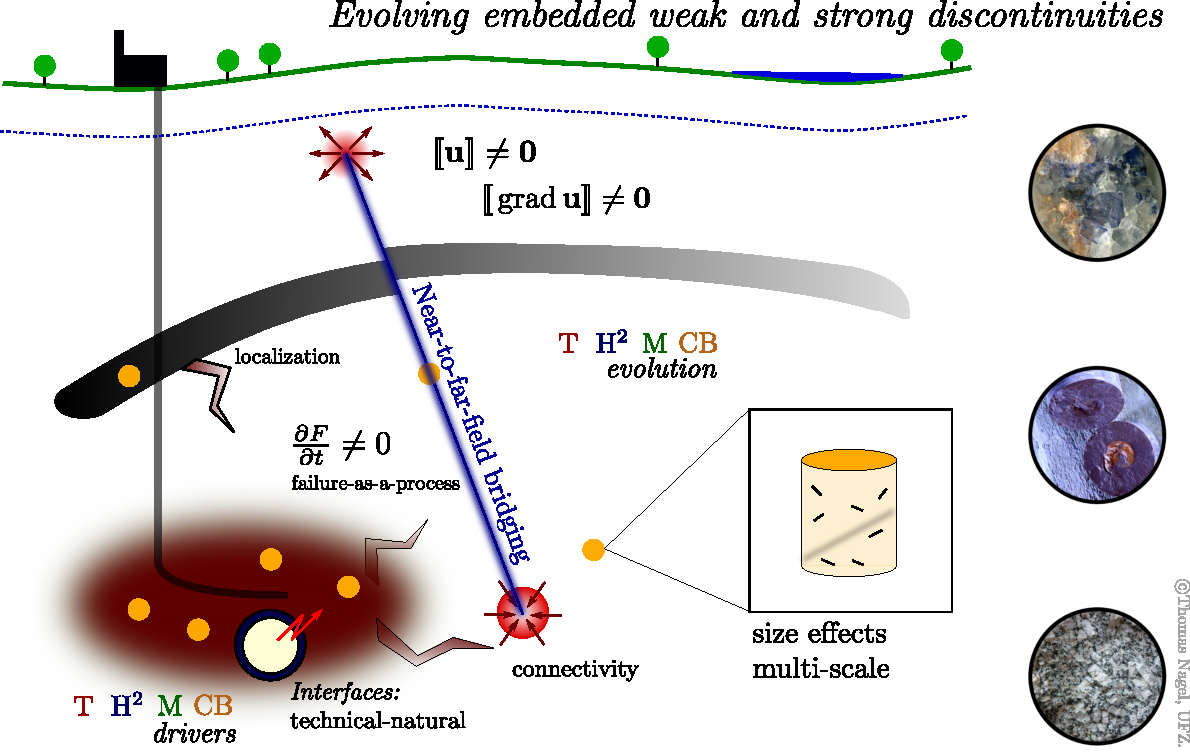
\includegraphics[width=1\textwidth]{figures/Barrier_concept.pdf}
\caption{Graphical abstract of the GeomInt project: geological reservoir-barrier systems and geomechanical integrity}
\label{fig:pro01}
\end{figure}

\section{The GeomInt project}
\label{sec:geomint}

GeomInt\index{GeomInt} (Geomechanical Integrity of Host and Barrier Rocks -- Experiment, Modeling and Analysis of Discontinuities) contributes to the realistic and application-oriented experimental-numerical analysis of the formation and development of discontinuities in underground rock salt\index{rock salt}, clay rocks\index{clay rock} and crystalline rocks\index{crystalline rock}. In the following, these rocks will also be briefly referenced as salt, clay and crystalline. The understanding and quantification of interactions with dynamically developing geological rock properties (e.g. permeability), which determine the geomechanical integrity\index{geomechanical integrity} and tightness of geological reservoir-barrier systems, are at the centre of this work. Included in the investigations are discontinuities of volumetrically distributed damage types as they occur in the damage zone of solid rocks, discontinuities that can form uncontrolled or controlled at phase boundary surfaces as well as discrete crack and fracture networks\index{fracture networks}. The pathways created or extended by these discontinuities for fluids in host and barrier rocks harbour the risk that, for example by migration of fluid phases from deep to near-surface geological strata and ultimately into the biosphere, vital ecosystems can be impaired significantly. A range of thermo-hydro-mechanical-chemical (THMC) processes\index{THMC processes} can cause an evolution of discontinuities in the near field of a geotechnical infrastructure. This in turn may lead to the establishment of previously not existent connectivity. When connectivity is established to conductive fault zones\index{fault zones} or fracture networks with a certain range, transport into the far field can become possible on a much shorter time scale than before (Fig.~\ref{fig:pro01}).

\begin{figure}[ht!]
\begin{minipage}{0.69\textwidth}
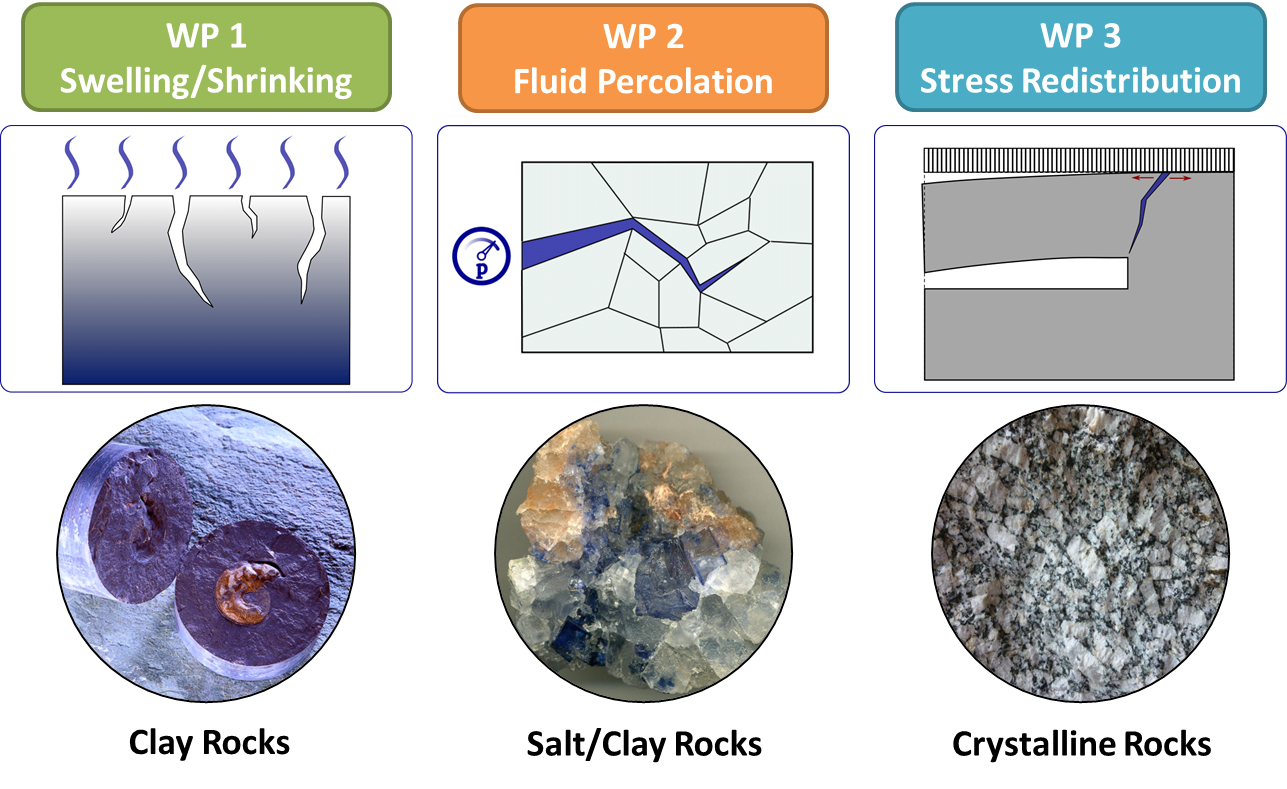
\includegraphics[width=1\textwidth]{figures/geomint-concept-02.png}
\end{minipage}
\hfill
\begin{minipage}{0.29\textwidth}
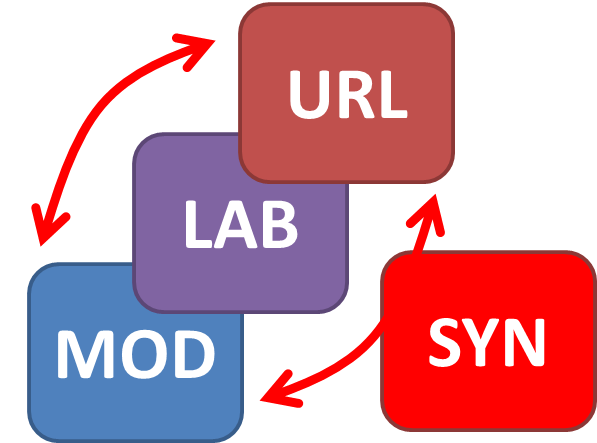
\includegraphics[width=1\textwidth]{figures/modal01a.png}
\end{minipage}
\caption{Work package structure of GeomInt according to process and rock types (left) and combining experimental as well as modelling works in a synergistic workflow (right)}
\label{fig:pro02}
\end{figure}

GeomInt is conducted by an interdisciplinary consortium of partners from universities, governmental and private research institutions with complementary, long-term experience in the analysis of underground geosystems. Three typical effects leading to the emergence and development of specific discontinuities are considered as main research areas: Swelling and shrinkage processes, pressure-driven fluid percolation and stress redistribution (Fig.~\ref{fig:pro02}). The research work is structured into laboratory experiments, numerical simulation and in-situ experiments (in underground research laboratories, URLs)\index{underground research laboratory}\index{URL}. New insights into process understanding have been gained from the laboratory experiments. In particular, contributions of coupled thermal, hydraulic, and mechanical (THM) processes for the formation and development of discontinuities have been considered. These findings have been used to support the further development of different continuum mechanical\index{continuum mechanics}, discontinuum mechanical\index{discontinuum mechanics} and hybrid numerical approaches\index{hybrid numerical approaches} and to compare their potentials and limitations. Novel models and algorithms have been implemented in scientific software mainly which is available to the research community. The suitability of the models for the analysis and prediction of realistic operating scenarios of underground geosystems (e.g. geothermal reservoirs, geological reservoirs for energy sources and waste) will be further validated on the basis of test field simulations of different in-situ experiments, which have been carried out primarily using synergies with other national and international research projects in underground laboratories accessible to project partners of GeomInt.
%
The process-oriented work packages are interlinked with synthesis activities such data and model integration using virtual reality (VR) methods (Fig.~\ref{fig:pro03})\index{Virtual Reality (VR)}. A corresponding pilot demonstrator is being implemented in the Mont Terri project.

\begin{figure}[ht!]
\begin{minipage}{0.49\textwidth}
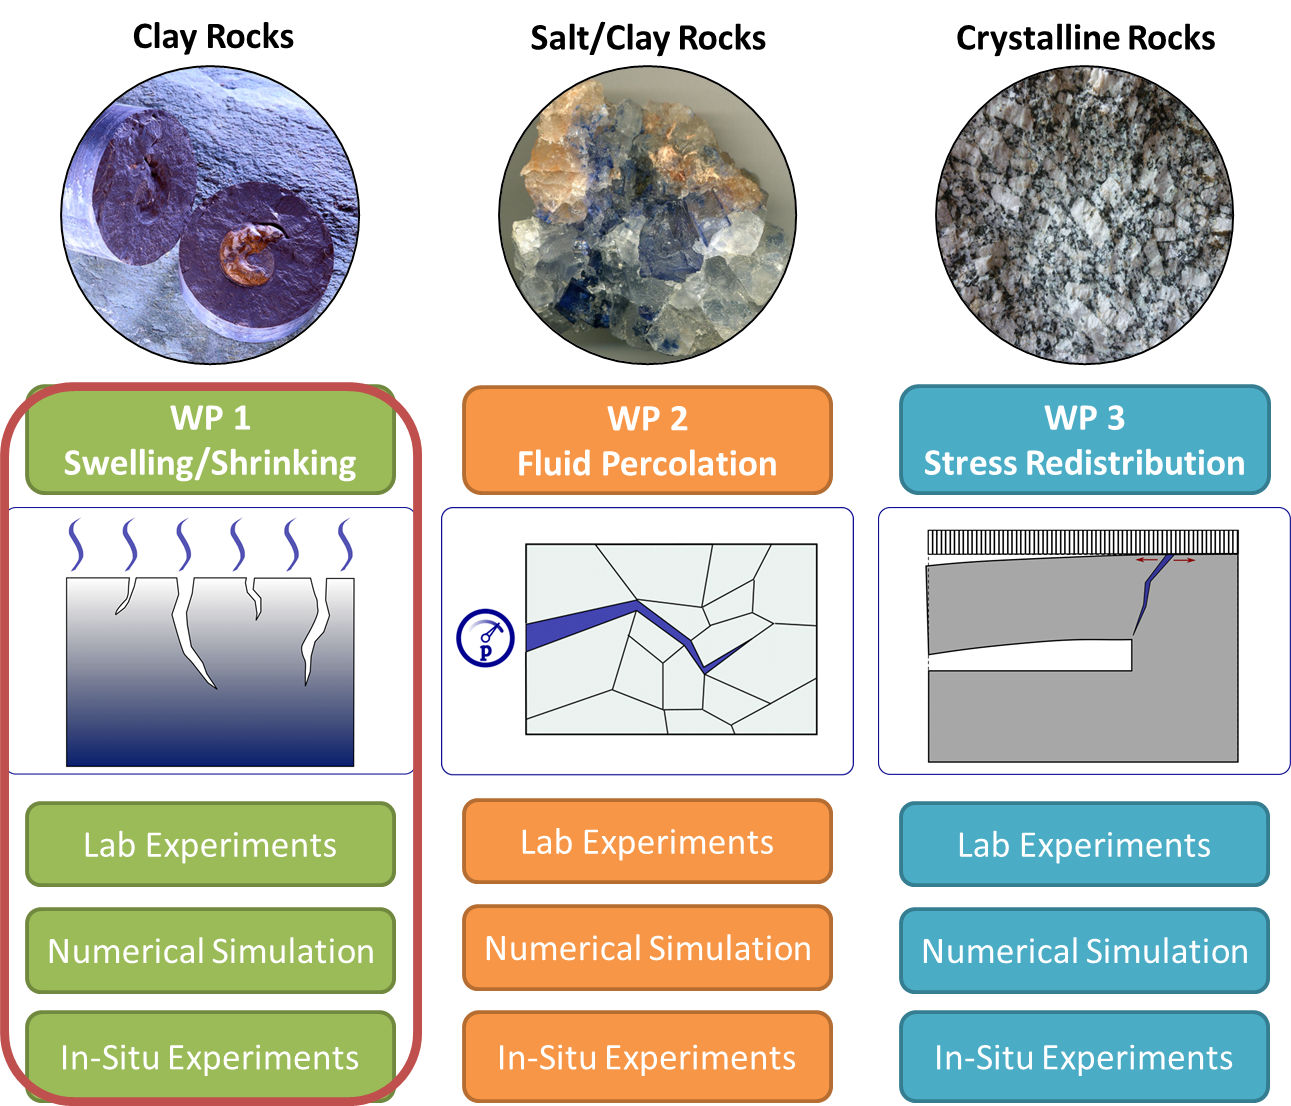
\includegraphics[width=1\textwidth]{figures/geomint-wp1a.png}
\end{minipage}
\hfill
\begin{minipage}{0.49\textwidth}
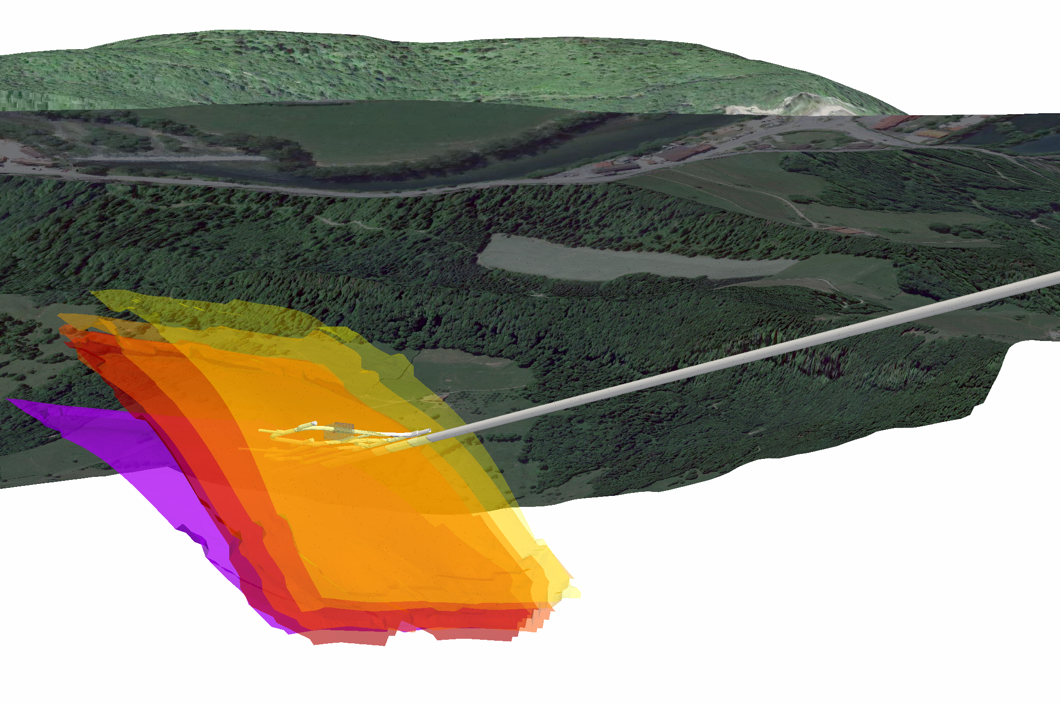
\includegraphics[width=1\textwidth]{figures/mt-vr-01.png}
\end{minipage}
\caption{Synthesis: Interlinking process-oriented work packages with VR methods (VR Mt. Terri - visual data and model integration)}
\label{fig:pro03}
\end{figure}

The project results allow an improved process understanding. The applied methods and the application-oriented systems for relevant time and length scales will support safer, more reliable and more efficient planning and realization of geotechnical applications. An important advantage of GeomInt is the principle transferability of experimental-numerical concepts, models and methods to a multitude of urgent scientific-technical questions in the geosciences. This allows the exploitation of project results for different politically and socially relevant geotechnological uses (e.g. deep geothermal energy, energy storage, repository problems, methods for hydraulic stimulation, conventional and unconventional resource extraction or tunnel construction). This transferability has been particularly taken into account in the methodological design of the project as well as in the documentation of methods, approaches and results and can at the same time serve as a basis for potential follow-up work to GeomInt.
\index{Virtual URL Mt. Terri}

\section{GeomInt approach: lab, in-situ, in-silico, virtual reality}\index{in-situ}\index{in-silico}

GeomInt relies on a very close link between experimental and modelling work. Three work packages focus on different mechanisms affecting the barrier integrity of potential host rocks: (WP1) swelling/shrinking of clays, (WP2) pressure driven fluid percolation in salt and clay rocks as well as (WP3) stress redistribution in crystalline rocks.
%
Fig.~\ref{fig:appraoch} illustrates the geographical WP workflows from in-situ sampling to geomechanical laboratories and modelling. The main sources for rock samples are (i) Mt. Terri for clay (ii) Springen for salt and (iii) Freiberg/Kirchberg for crystalline rock specimen. Moreover, there is collaboration with other URLs (Bure, Grimsel) concerning experimental and modelling work -- mainly for testing transferability of the methodology to other rock types (e.g. Callovo-Oxfordian Clay - COx).
\index{URL Mt. Terri}
\index{URL Reiche Zeche}
\index{URL Bure}
\index{URL Grimsel}
\index{COx Callovo-Oxfordian Clay}

\begin{figure}[ht!]
\centering
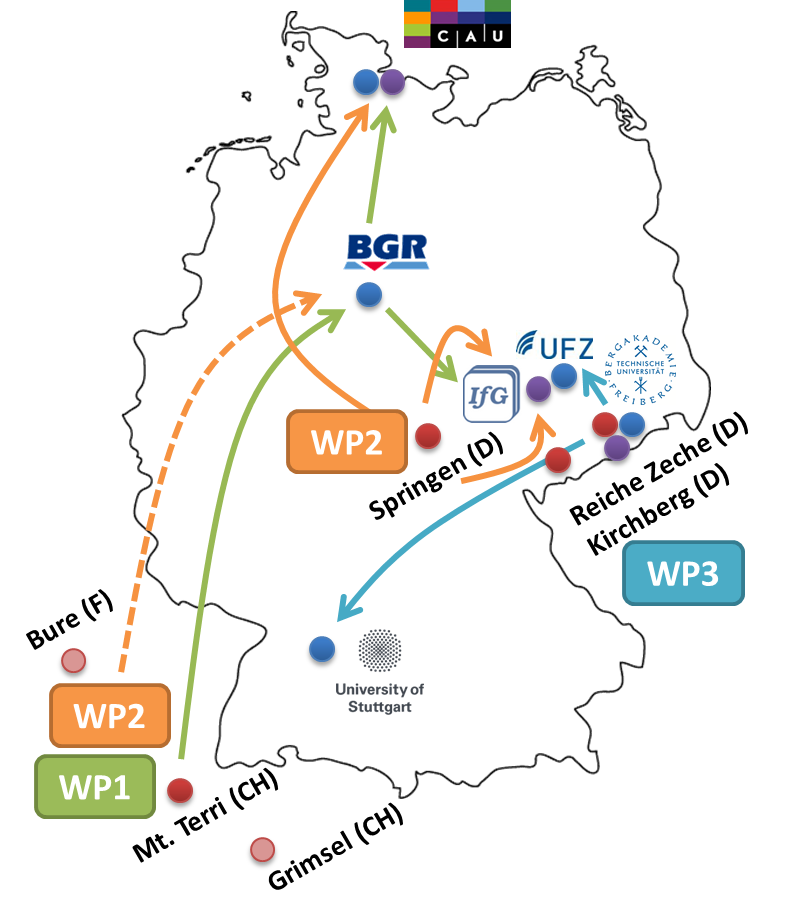
\includegraphics[width=0.8\textwidth]{figures/geomint-all.png}
\caption{Geographical work flow including interlinked experimental and modeling works in GeomInt}
\label{fig:appraoch}
\end{figure}

In the following we briefly introduce the ''geographical workflow'' for the individual work packages. Please not that the experimental and modelling platforms for the analysis of discontinuities are being established independent of specific rock types.

\begin{figure}[ht!]
\begin{minipage}{0.48\textwidth}
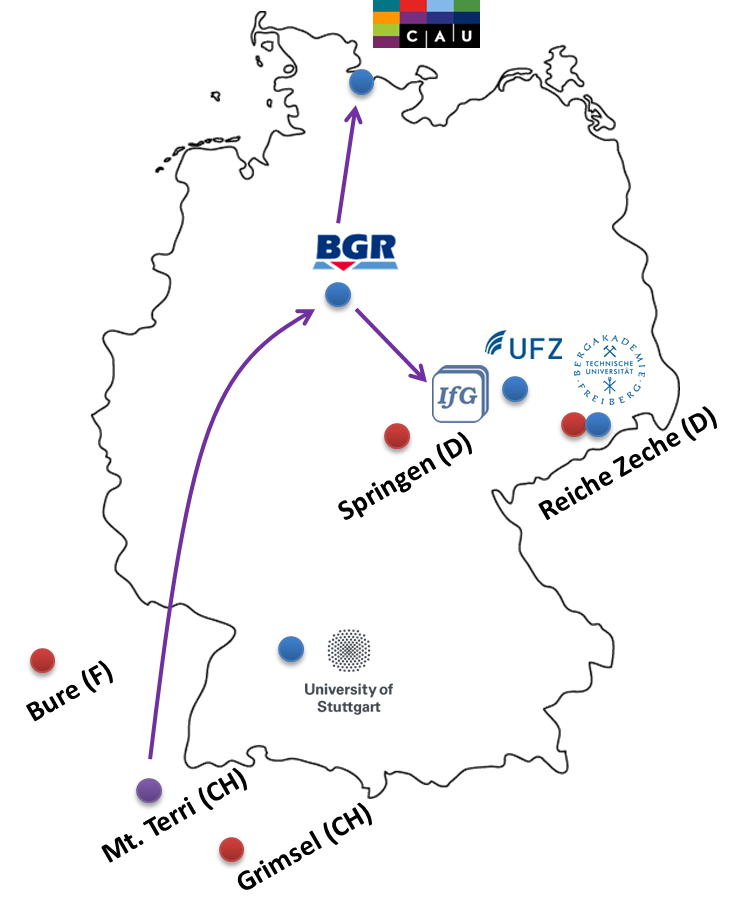
\includegraphics[width=\textwidth]{figures/geomint-wp1.png}
\caption{WP1: Swelling / shrinking}
\end{minipage}
\hfill
\begin{minipage}{0.48\textwidth}
WP1 is dealing with swelling and shrinking processes in clay stone. BGR obtains \textbf{Opalinus Clay} samples from the Mont Terri Underground Research Lab (URL) in Switzerland and providing them for laboratory testing to CAU and IfG partners in Kiel and Leipzig, respectively. Samples come from various clay and sandy facies. Experimental work with specimen from the sandy facies is particularly challenging due to the large heterogeneity of the material. WP1 is closely linked with the Mont Terri Project in cooperation with swisstopo.\index{Opalinus Clay}
\end{minipage}
\end{figure}

\begin{figure}[ht!]
\begin{minipage}{0.48\textwidth}
Fluid percolation processes are studied in both \textbf{clay and salt rocks}, i.e. ductile materials. Samples of Opalinus Clay come from the Mt. Terri URL (see above). Salt rock samples are mainly obtained from the Springen site in Thuringia. Experimental works concerning percolation are conducted in the IfG and CAU labs in Leipzig and Kiel. WP2 investigates mechanisms of percolation threshold for both rock types depending on hydro-mechanical (HM) processes (i.e. fluid pressure and mechanical stress field).
\end{minipage}
\hfill
\begin{minipage}{0.48\textwidth}
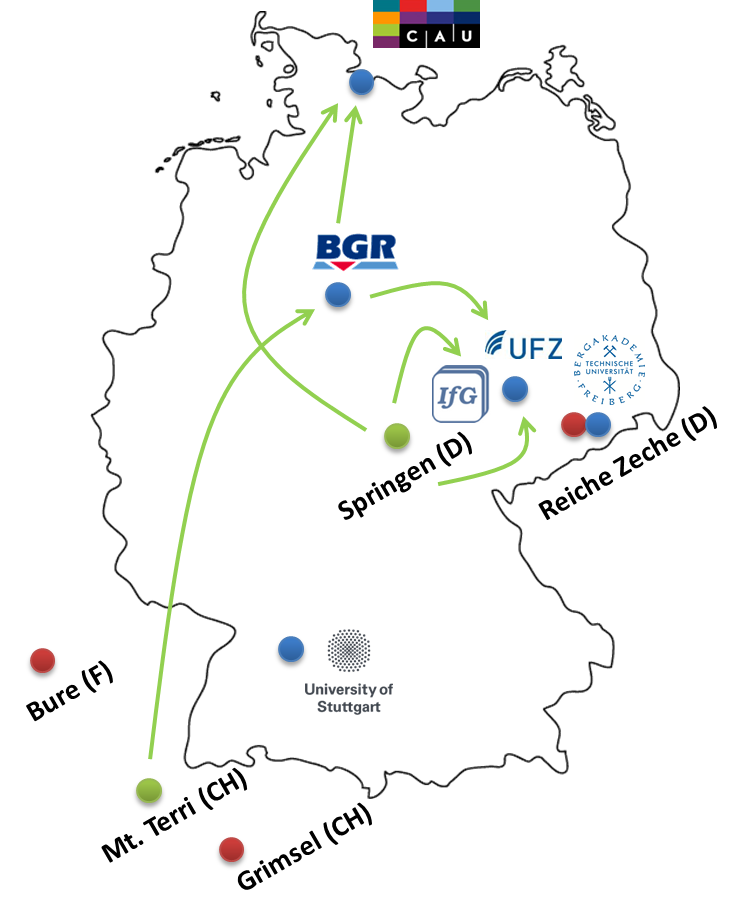
\includegraphics[width=\textwidth]{figures/geomint-wp2.png}
\caption{WP2: Fluid percolation}
\end{minipage}
\end{figure}

\begin{figure}[ht!]
\begin{minipage}{0.48\textwidth}
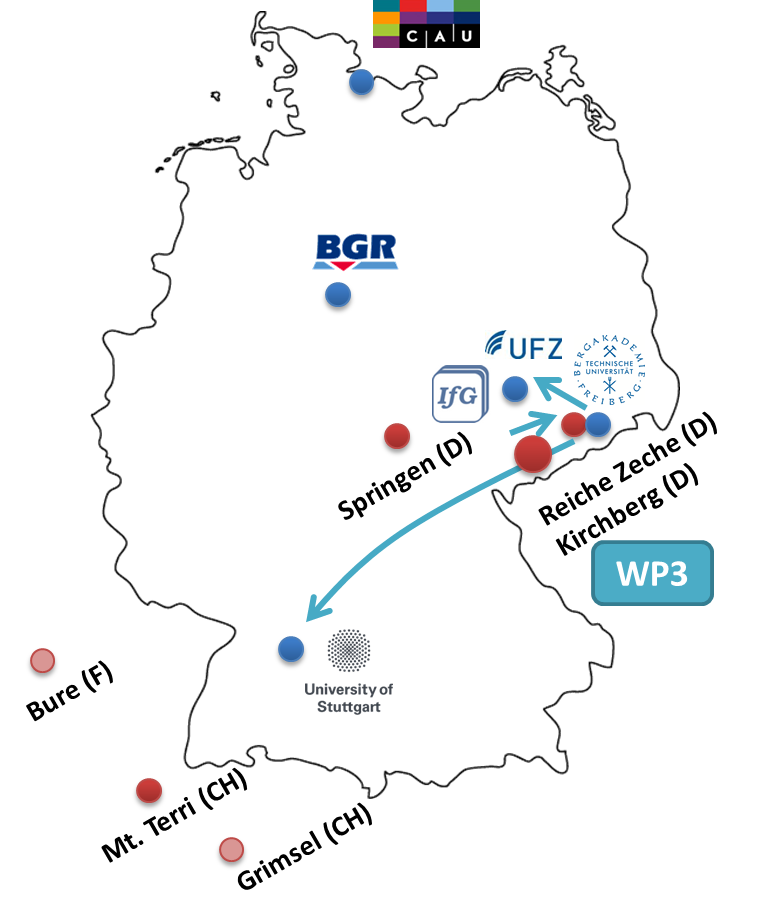
\includegraphics[width=\textwidth]{figures/geomint-wp3.png}
\caption{WP3: Stress redistribution}
\end{minipage}
\hfill
\begin{minipage}{0.48\textwidth}
WP3 is investigating discontinuities formed by stress redistribution in brittle materials. \textbf{Granite rock} samples are obtained from locations in the Ore Mountains, i.e. from Kirchberg and Freiberg (URL Reiche Zeche). Experimental  investigations are conducted in the Freiberg (TU Freiberg) and Stuttgart labs (University of Stuttgart). Constant Normal Load (CNL) and Constant Normal Stiffness (CNS) experiments are conducted to study fluid flow in rough fractures under confining stresses. Rock samples from Freiberg will be also used with in the ''Crystalline Task'' of the new DECOVALEX-2023 phase.
\index{Constant Normal Load (CNL) experiment}
\index{Constant Normal Stiffness (CNS) experiment}
\index{DECOVALEX}
\end{minipage}
\end{figure}

Output from the following research infrastructures will be combined:
\begin{itemize}
    \item \textbf{Rock-mechanical laboratories}
	\begin{itemize}
		\item THM-coupled testing under controlled boundary conditions
		\item Material and process characterization
	\end{itemize}
	\item \textbf{Numerical methods and software}
	\begin{itemize}
		\item OpenGeoSys (XFEM, PFM)
		\item md-LEM (LEM)
		\item pythonSPH (SPH)
		\item UDEC, 3DEC (DEM)
		\item FLAC3D (FDM)
	\end{itemize}
	\item \textbf{Underground laboratories}
	\begin{itemize}
		\item Springen (rock salt, potash)
		\item Mont Terri (clay rock)
		\item Reiche Zeche (crystalline rock)
	\end{itemize}
	\item \textbf{Simulation- and development infrastructure}
	\begin{itemize}
		\item HPC Cluster
		\item Version management
		\item VISLAB (\url{www.ufz.de/vislab})
	\end{itemize}
\end{itemize}

In addition to experimental (lab and in-situ) and modelling work, we use Virtual Reality (VR) methods for data and model integration as well as visualization. Fig. \ref{fig:vr-url} shows a snapshot of the Virtual URL project for Mont Terri. The basic idea is to combine all information from in-situ (and even lab) experiments as well as the corresponding models in a Virtual Reality context - like a visual data base. VR embedded data can be accessed in an interactive and interoperable manner \cite{Rink2020}.
\index{HPC High-Performance-Computing}
\index{VISLAB}

\begin{figure}[ht!]
\centering
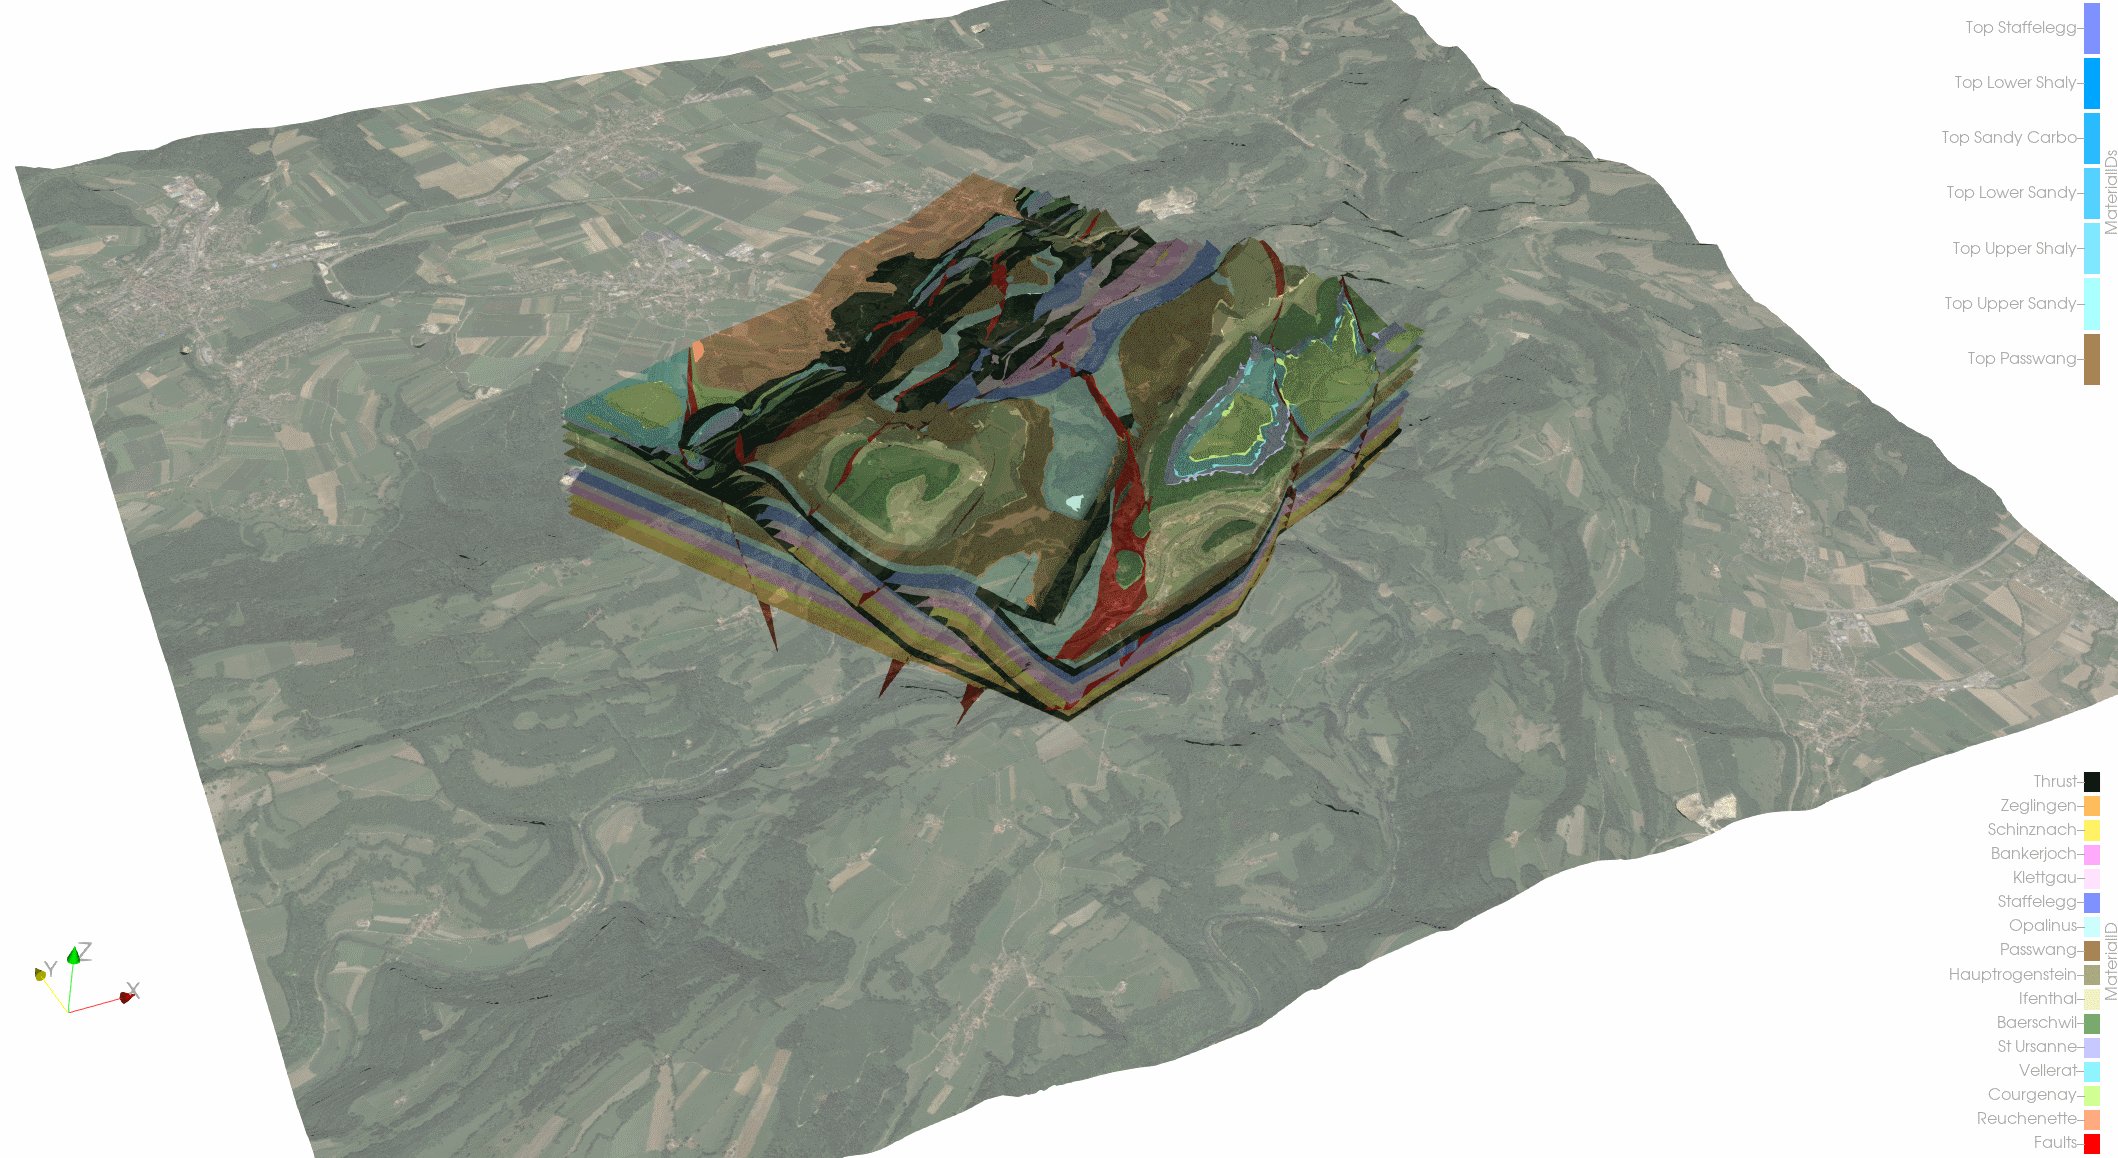
\includegraphics[width=0.9\textwidth]{figures/mt-surface+move.png}
\caption{Virtual URL Mont Terri: Virtual data and model integration in a precise geo-referenced context}
\label{fig:vr-url}
\end{figure}

\bigskip
\hrule
\bigskip

The book is organized in the following way:
Experimental and modelling platforms are described in detail in Chapter \ref{cha:exp} and \ref{cha:num}, respectively. It follows the ''Model-Experiment-Exercises'' (MEX) combining experimental and modeling work for a ''Proof-of-Concept'', i.e. are experiments and models adequate to better understand fracturing processes in various rock types (Chapter \ref{cha:mex}). The Data-Management concept is introduced in Chapter \ref{cha:dms} accompanied by examples for data and model storage. The book end with a synthesis and outlook Chapter (\ref{cha:out}). Lists of symbols, literature references, keywords (index) can be found in the appendices.
\index{MEX Model-Experiment-Exercise}
\index{PoC Proof-of-Concept}

\clearpage
%--------------------------------------------------------------------
\section{GeomInt team}
\label{sec:team}

The GeomInt consortium is made up of the partners Federal Institute for Geosciences and Natural Resources, Christian-Albrechts-University of Kiel, Helmholtz Centre for Environmental Research - UFZ, Institut f\"ur Gebirgs\-mechanik GmbH, TU Bergakademie Freiberg and University of Stuttgart. The consortium is based on the complementary expertise and resources of the partners, partly unique laboratory equipment, many years of experience with different numerical approaches and access to underground laboratories for the rocks under consideration. Detailed information on the partners and their previous project-relevant work is presented in the following.

\subsection{BGR}
\begin{wrapfigure}{r}{2cm}
\centering

\includegraphics[width=2cm]{./figures/BGR_Logo.png}
\end{wrapfigure}
The Federal Institute for Geosciences and Natural Resources (BGR, Germany) is the central consulting institution for the German federal government for all geoscientific questions, inter alia the safe final disposal of radioactive waste and the related geological-geotechnical safety analyses. As such, the BGR with its wide-ranging experience has an interest in investigating the host rocks salt, claystone and crystalline rocks to guarantee an independent recommendation for the site selection process. This includes the use of state-of-the-art modelling and experimental techniques. Within the GeomInt project, the BGR is focusing on the integrity of clay rock formations as they are currently investigated in the Mont Terri Underground Rock Laboratory (URL) in Switzerland. The BGR is currently coordinating and participating in several experimental campaigns that are expected to enhance the fundamental understanding of clay rock exposed to stress redistribution, seasonally varying boundary conditions and pressure driven percolation. For the simulation of the hydraulic conditions of unsaturated claystone coupled with unsaturated linear elastic mechanical deformation, a strong collaboration with the Helmholtz Centre for Environmental Research (UFZ) has been pursued to employ the open source code OpenGeoSys for in-situ scale problems of the Mont Terri URL.

\subsection{CAU}
\begin{wrapfigure}{r}{2cm}
\centering

\includegraphics[width=2cm]{./figures/cau_logo.png}
\end{wrapfigure}

The geomechanical and geotechnical group of Christian-Albrechts-University (CAU) of Kiel has vast experience in the experimental and numerical analysis of coupled thermo-hydro-mechanical (THM) processes in geomaterials. Some research fields which are under investigation and development at CAU Kiel are: material characterization by static, cyclic and dynamic loaded soil-structure-interaction, development of sustainable geomaterial and earth structure, material characterization by geophysical and advanced geotechnical methods, energy geotechnics, energy geo-storages, and cyclic thermo-hydro-mechanical loaded geomaterial. In 2016, the first international conference on energy geotechnics (ICEGT-2016) was organized and hosted in Kiel University. The numerical simulations such as Coupled hybrid models, boundary element modeling (BEM), finite element modeling (FEM), static and dynamic soil-structure-interface and constitutive modeling, cyclic system / macro modeling for complex soil-structure-conditions and loads as well as fracture simulation under coupled THM processes using lattice element method (LEM) have all been developed here and have been applied in different research fields and projects, such as ANGUS, DuoFill, FIBERSLAG, BioSolidEncap and GeomInt.

\subsection{IfG}
\begin{wrapfigure}{r}{2cm}
\centering

\includegraphics[width=2cm]{figures/logo-ifg-klein.png}
\end{wrapfigure}
The Institut f\"ur Gebirgsmechanik GmbH - IfG is one of the leading companies for all questions regarding the use of salt formations, e.g. salt mining, storage, and waste disposal projects. We adopt an interdisciplinary approach, consisting of numerical and experimental geomechanics, as well as geotechnical in in-situ field measurements. The company provides fundamental geomechanical/geotechnical safety concepts, and produces evidence reports on rock-mechanical stability and long-term safety in the form of design concepts, site planning procedures and public acceptance procedures. Supported by combinations of in situ observations, 
geomechanical laboratory testing and numerical modelling we provide comprehensive expertise in rock mechanics, necessary to solve practical mining or repository problems and to reduce project risks. Our research includes such diverse phenomena like creep, strain softening and post-failure behavior, rock burst mechanisms, and pressure-driven percolation in polycrystalline salt rocks (both numerically and experimentally). Overall, the IfG can draw on more than five decades of continuous application of research in the field of rock mechanics.

\subsection{TUBAF}
\begin{wrapfigure}{r}{2cm}
\centering

\includegraphics[width=2cm]{figures/TUBAF_Logo_orig_RGB}
\end{wrapfigure}
The Technical University of Freiberg as so called "University of Resources" focuses on energy, resources and materials. The institute of geotechnical engineering works in the field of using the crust of the earth. This affects topics like radioactive waste repositories in different host rocks (salt, crystalline, clay), geothermal energy production, gas storage or tunneling. To face this challenges the results of the rock mechanical laboratory, the "Reiche Zeche" (the local research mine) and numerical simulations are used. Involving practical and numerical results on different scales helps to give a useful contribution to open questions in the related research topics. The staff of the institute works in different national and international research projects. The topic of deep geothermal energy is on the agenda since 2008. Particularly the genesis and development of cracks and crack formations was intensively studied. E.g. the hydraulic fracturing, the induced seismicity or the response of existing cracks to static and dynamic loads have been experimentally and numerically investigated.  

\subsection{UFZ}
\begin{wrapfigure}{r}{2cm}
\centering

\includegraphics[width=2cm]{figures/ufz}
\end{wrapfigure}
The Helmholtz Centre for Environmental Research - UFZ deals with a variety of tasks in environmental, climate and energy research, the results of which are internationally recognized. In the energy sector, the spectrum of topics covered ranges from process modelling and simulation to the development of innovative monitoring strategies and the investigation of socio-economic aspects. Since its foundation in 2007, the Department of Environmental Informatics (ENVINF) has been concerned with the development of numerical methods and software components for the simulation of coupled processes in porous media based on the finite element method. In addition, the development of simulation platforms for the treatment of these problems as well as benchmarking for model and software validation will be discussed. Workflows and system components for the 3D visualization of complex, heterogeneous data from different sources are an integral part of these platforms. In this context, the UFZ acts as main developer and coordinator of the international scientific open source software project OpenGeoSys. In addition to method and software development, there is a strong connection to applications in hydrology, geotechnics and energy storage research. Aspects of modelling and numerical simulation of discontinuities in rocks were considered in phase field, non-local deformation and modified XFEM approaches, especially in connection with process analysis in Enhanced Geothermal Systems. In order to increase the efficiency of numerical simulations and for the clear evaluation of results, the UFZ has capacities for high-performance computing and scientific 3D visualization. 

\subsection{UoS}
\begin{wrapfigure}{r}{2cm}
\centering

\includegraphics[width=2cm]{figures/unistuttgart_logo.png}
\end{wrapfigure}
The Institute of Applied Mechanics (Chair of Continuum Mechanics) at the University of Stuttgart (UoS) contributes with a profound knowledge of coupled geomechanical problems in different scales. Investigations in the field of subsurface flow in fractured and unfractured porous media to answer open questions regarding underground storage, geomaterial characterization and geotechnical energy and safety concerns is just a small selection of the overall research fields of interest. Experimental state of the art infrastructure including a custom designed $\mu$XRCT-Scanner with for image-based characterization combined with hydro-mechanical in-situ experiments, imaging and PIV of complex single and multi-phase flow processes in micro-fluidic setups with sub-micrometer pore-scale resolution and various experimental devices for the harmonic characterization of complex fluids, solids, and especially rock (and granular media) samples form the basis of the so called Porous Media Lab(oratory) at UoS. The tight interplay of experimental and theoretical work is closed by a number of advanced numerical in house codes such as the solver package HOOSPH (based on the HOOMD-blue library), a massive parallel CPU/GPU Smoothed Particle Hydrodynamics (SPH) framework, PANDAS a general Finite Element (FE) package for strongly coupled multiphasic porous media problems, and a newly developed extension of the DUNE PDELab framework for coupled problems in fractured porous media using hybrid-dimensional element formulations. Important contribution of the experimental and numerical work in numerous projects within the CRC 1313 at University of Stuttgart (https://www.sfb1313.uni-stuttgart.de), GeomInt (https://www.ufz.de/geomint/), SHynergie and the Cluster of Excellence SimTech (https://www.simtech.uni-stuttgart.de) help to prove the deep understanding of geomechanical processes.
%==============================================================================
%\part{Experimental Methods}
\todol{Experimental Platform-------------------------------------------------------------}
\chapter{Experimental Platform}
\label{cha:exp}
\Authors{BGR, Amir Shoarian Sattari (CAU), Mathias Nest, Dirk Naumann, TUBAF, UoS}
%\todo{Please insert authors}

In order to investigate the barrier rocks, such as saltstone, claystone and crystalline, response under the coupled thermo-hydro-mechanical (THM) processes, a series of laboratory and field tests in the scope of the GeomInt project are carried out. A graphical abstract of experimental activities is depicted in Fig. \ref{fig:appraoch}.

Initially, an introduction to the tested barrier rocks specifications and characteristics is provided (sec. \ref{sec:material-properties}). Next, the Opalinus claystone and saltstone responses under the coupled THM processes are investigated. Three-point bending, Brazilian disk and true triaxial tests are used to determine fracture toughness, splitting strength as well as changes of the mechanical and thermal properties under the coupled loadings, respectively. It is shown that the embedded layering orientation in the claystone samples has a significant effect on materials strength, deformation and frack paths (sec. \ref{sec:thm-lab-tests}).
%
After determining the general material properties, distinct laboratory tests, which are chosen based on the unique purpose of the GeomInt project, are performed to analyze the shrinkage and swelling behavior of the claystone samples under free or in-situ loading conditions. The results again indicate the effect of the anisotropy on the swelling and shrinkage direction of the claystone material (sec. \ref{sec:lab-wp1}). 
%
The fluid or gas driven percolation tests on Opalinus claystone and saltstone samples explore the change of the permeability, the required fracking pressure and the principle stress dependent frack paths. Additionally, the healing and frack closure characteristic of the barrier rocks are investigated. Moreover, the effect of the compressibility on the fluid flux and drop of the reservoirs pressure when using brine or gas as fracking medium is presented (sec. \ref{sec:lab-wp2}).
%
The direct shear test on the crystalline gives an insight of the shear characteristics of the joints under the constant normal load (CNL) boundary condition. Additionally, the constant normal stiffness (CNS) test with the additional of extra load to the CNL procedure is performed. Specifically, for the crystalline samples, the diffusion and time-dependence states of the fractures under the cyclic loading conditions are characterized. Eventually, the flow and pressure dependency on the deformations of the frack volumes and paths are studied (sec. \ref{sec:lab-wp3}).
\index{CNL Constant Normal Load experiment}
\index{CNS Constant Normal Stiffness experiment}

\begin{figure}[!ht]
\centering
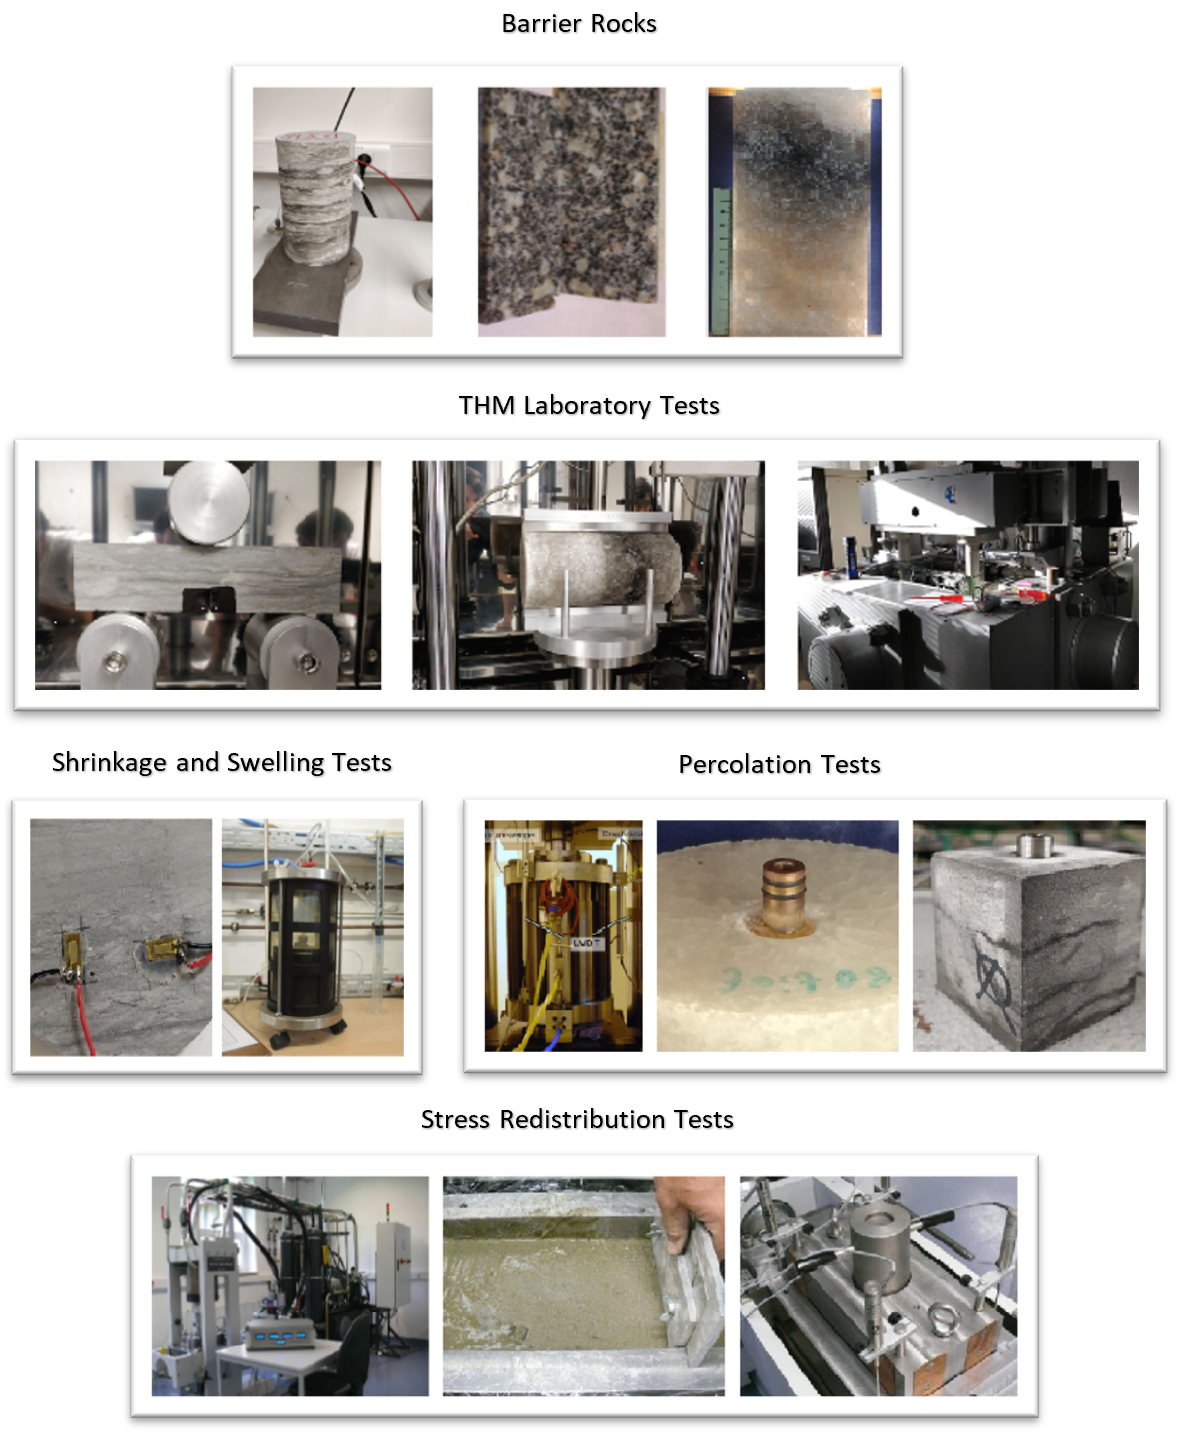
\includegraphics[width=0.95\textwidth]{figures/Amir_Experiment.png}
\caption{The conducted laboratory tests in the scope of GeomInt research project}
\label{fig:Amir_Experiment}
\end{figure} 
%===================================================================================================
\section{Rock Material Properties}
\label{sec:material-properties}
%-----------------------------------------------------------
\subsection{Opalinus Clay from Mont Terri, Switzerland}
\label{subsec:clay}
\Authors{Tilo Kneuker, Bernhard Vowinckel, Markus Furche, Gesa Ziefle, Jobst Ma{\ss}mann}

\subsubsection{The Mont Terri Rock laboratory}\label{sec:mont_terri}
\index{URL Mont Terri}
\index{Opalinus Clay}

Opalinus claystone is a very promising hostrock for the safe disposal of heat emitting nuclear waste. This type of hostrock has been investigated in the Mont Terri Rock laboratory for more than 24 years. The Mont Terri rock laboratory is a facility to conduct research in the deep geological underground at in-situ scale, such as the safe deposition of radioactive waste, where the local host rock is Opalinus Clay. The rock laboratory is located within the Jura Mountain fold belt. The development of the Jura fold belt began in the Middle Miocene around 12 million years ago, which was constrained by the first occurrence of overthrusted and folded molasse sediments \cite{bolliger1993}. The overthrust of the frontal fold and thrust belt over the allochthonous foreland (Tabular Jura) occurred ca. 10.5 million years ago \cite{becker2000}. More specifically, the Mont Terri rock laboratory is located in the southeast dipping fold limb of the NW-vergent Mont Terri anticline \cite{nussbaum2011}. The total amount of shortening of the anticlinal structure is approximately 2.1 km \cite{freivogel2003}. During the folding process, the northwestern fold limb of the Mont Terri anticlinal structure was sheared-off and now lies on top of the Tabular Jura (Figure \ref{fig:bgr_mt_sideview}). The Mont Terri anticlinal structure developed in a special structural setting at the intersection between the frontal part of the Jura fold belt (main shortening direction NW-SE) and the roughly N-S oriented structural elements of the Rhine-Bresse-graben transfer zone \cite{nussbaum2011}.

\begin{figure}[!ht]
\centering
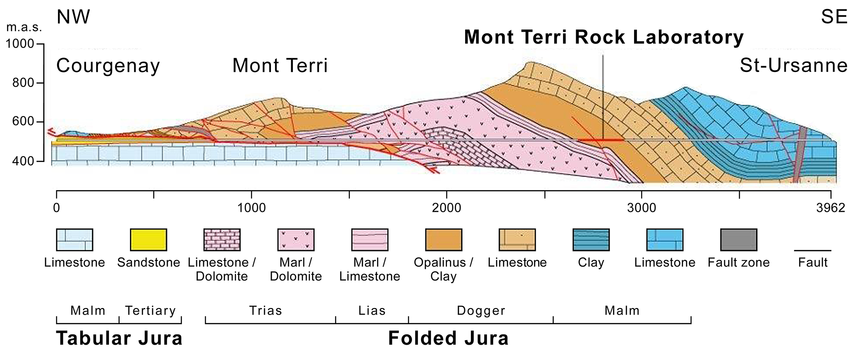
\includegraphics[width=1\textwidth]{./figures/bgr_mont_terri_side_view.png}
\caption{Geological cross section along the motorway tunnel through the Mont Terri anticline. From: Kaufhold et al. (2016) \cite{kaufhold2016}, based on Freivogel \& Huggenberger (2003) \cite{freivogel2003}.}
\label{fig:bgr_mt_sideview}
\end{figure}

The Mont Terri rock laboratory branches off from the security gallery of the motorway tunnel near the town of St. Ursanne (NW Switzerland). The rock laboratory is located mainly within the Middle Jurassic Opalinus Clay formation. The thickness of the Opalinus Clay in the rock laboratory is around 130 m \cite{hostettler2018} and the layers are dipping with ca. 40° towards SE. The depth below ground varies between 230 m and 320 m, depending on the topography \cite{heitzmann2001}. Since 1996, a total of 1400 m of galleries and niches have been excavated in the Mont Terri rock laboratory (Figure \ref{fig:bgr_mt_topview}). The Mont Terri rock laboratory is a generic scientific research laboratory. At Mont Terri, there will be no storage of radioactive waste.

\begin{figure}[!ht]
\centering
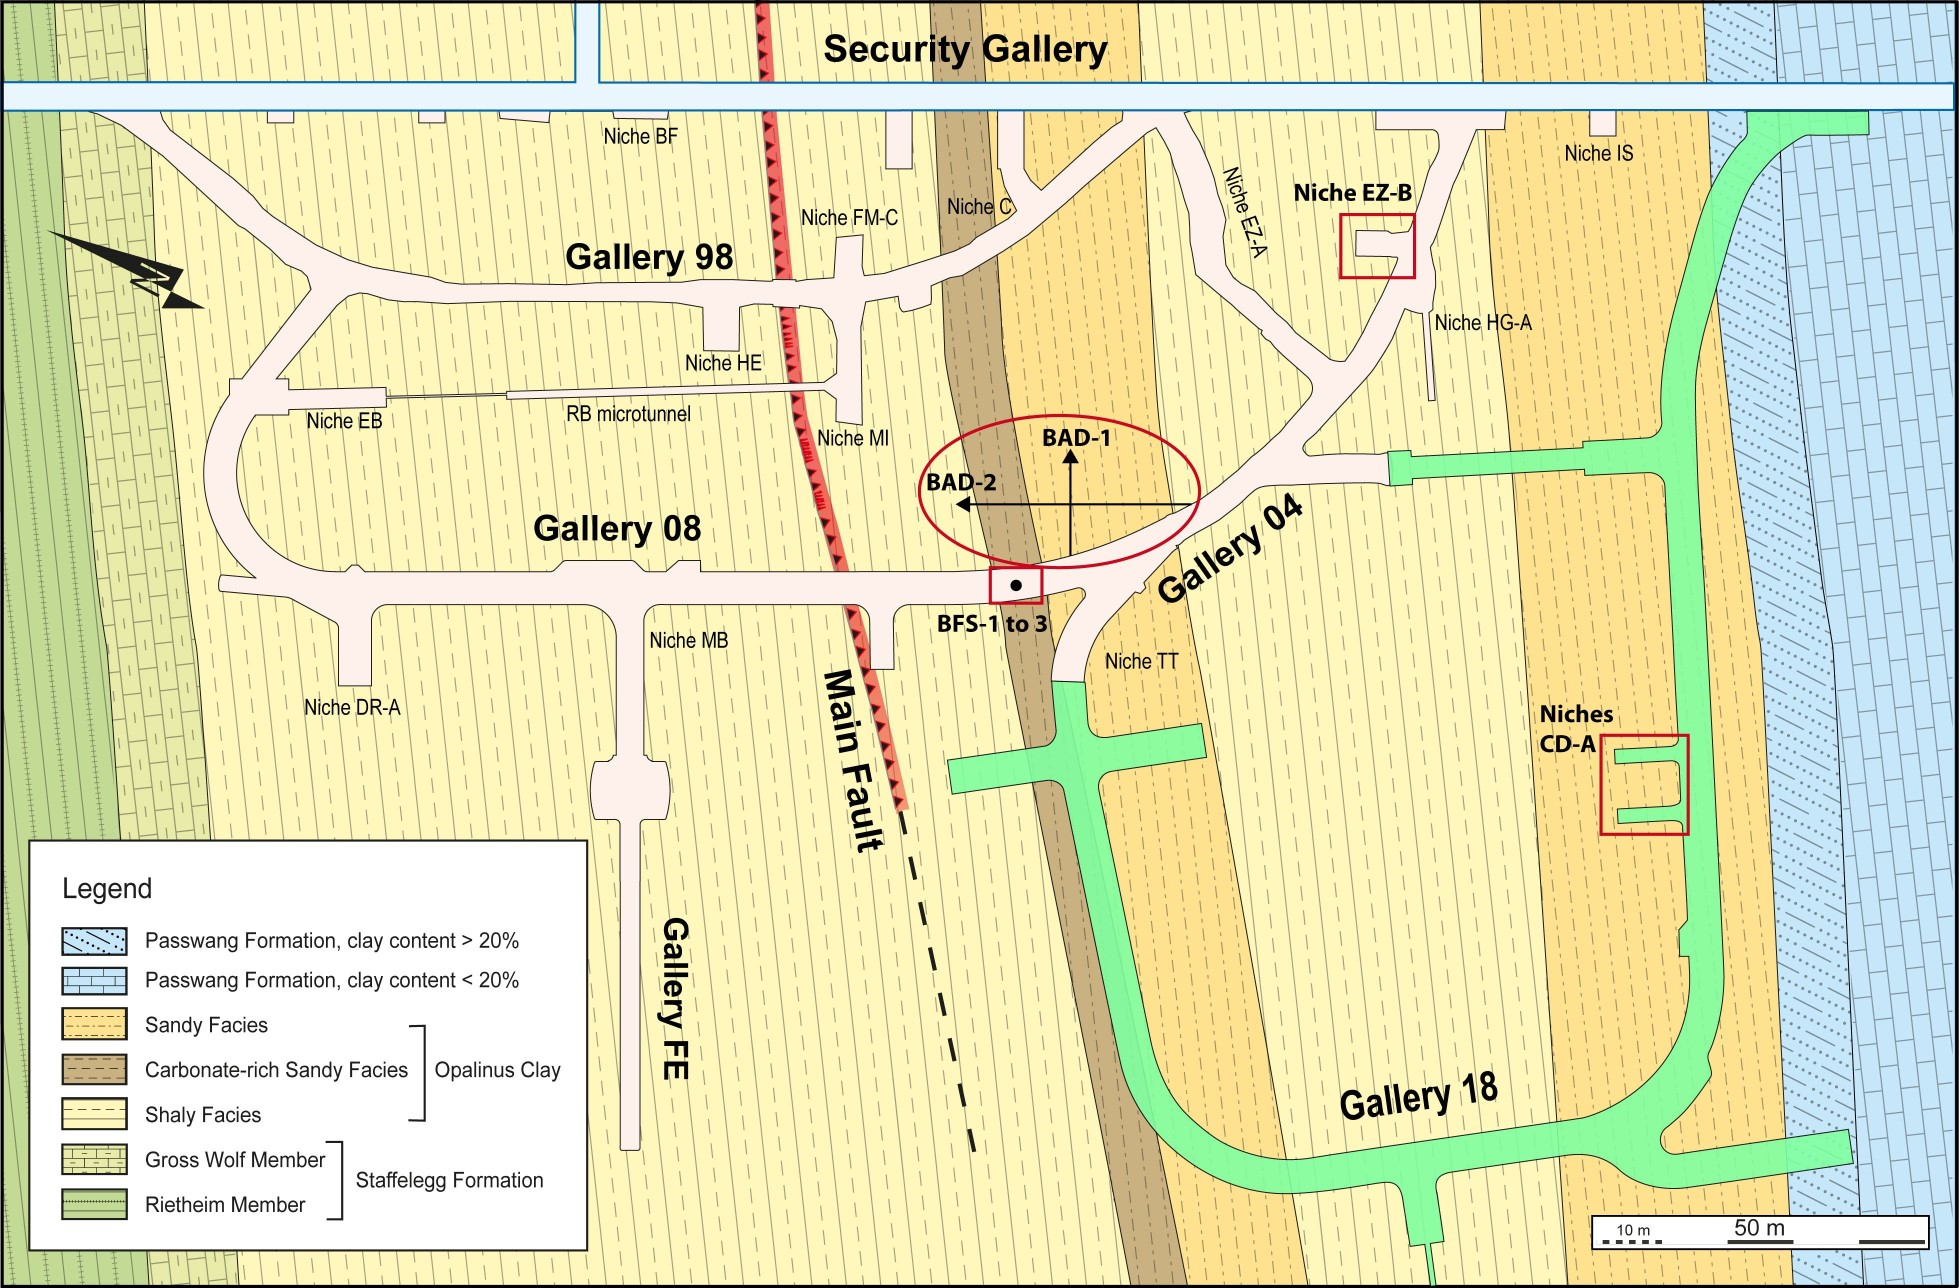
\includegraphics[width=1\textwidth]{./figures/bgr_mont_terri_top_view.jpg}
\caption{Geological map of the rock laboratory with all in-situ experiments relevant for the GeomInt project including the locations of the two AD-boreholes (BAD-1, BAD-2), the drilling for the FS experiment (BFS-1 to 3), the EZ-B niche for the CD/LP experiment and its successor experiment CD-A in Gallery 18. The different facies types of the Opalinus Clay can be recognized by the different shades of brown and yellow, the new Gallery 18 and the new experiment niches are highlighted in green on the map.  (map modified from Mont Terri Consortium, swisstopo).}
\label{fig:bgr_mt_topview}
\end{figure}
\index{MT-CD/LP experiment}
\index{MT-FS experiment}

The Opalinus Clay in the rock laboratory is composed of a dark gray claystone that was named after the ammonite species Leioceras opalinum. This claystone formation was deposited during the period of the Toarcian/Aalenian, at an age of approximately 174 million years. The Opalinus Clay is exposed along the rim of the Swabian and Franconian Alp in Germany and stretches into northern Switzerland \cite{einsele1983}. The Opalinus Clay was deposited in a shallow-marine, epicontinental milieu in the area of the storm wave base at approximately 20 m to 50 m water depth \cite{wetzel2003}. Coarser siliciclastic components are of detritical origin. Potential sources for the detritic components are the areas of the Bohemian Massif and the Vindelician Landmass \cite{wetzel2003}. During Cretaceous burial, the Opalinus Clay experienced maximum palaeo temperatures of $75^{\circ}$~C to $90^{\circ}$~C \cite{bossart2008} at a maximum burial depth of 1.35 km. The Opalinus Clay at the Mont Terri site is underlain by  marls of Upper Toarcian age and overlain by limestones (Bajocian), some of which act as karst aquifer \cite{pearson2003}.
\index{karst aquifer}

The Opalinus Clay at the Mont Terri rock laboratory can be subdivided into three main facies types \cite{bossart2008}. First, the lower shaly facies occupies the largest area of the rock laboratory (Figure \ref{fig:bgr_mt_topview}). It dominates the lower part of the Opalinus Clay formation. It consists of mica-bearing clay and marly shales as well as flasery, marly layers characterized by bioturbation. The upper shaly facies contains a higher volumetric content of quartz grains. Second, the sandy facies occurs in the middle and upper part of the profile (lower and upper sandy facies). It includes medium gray marly claystones with intercalated, bioturbated marly layers or lenticular, gray sandy limestones and pale sand layers of approximately 1-10 mm thickness that include pyrite as well. Third, a carbonate-rich sandy facies of approx. 5 m thickness occurs in the middle part of the rock formation. It consists of calcareous sandstones with intercalated bioturbated limestone layers, which show a relatively high proportion of detritic quartz and white mica. The different facies types of the Opalinus Clay can be attributed to varying sedimentation conditions in a shallow marine environment (like variations in depth and current directions). The carbonate-rich facies is typical for the Jura region in western Switzerland and it does not occur in the proposed siting regions for a deep geological repository in Northern Switzerland.
\index{bioturbation}

The mineralogical composition of the Opalinus Clay was examined by Traber \& Blaser (2013) \cite{traber2013} for several locations in Northern Switzerland. For the shaly facies, the clay mineral content varies between 40 wt\% and 75 wt\%. The clay minerals determined include illite, kaolinite and smectite-illite mixed layer minerals, the proportion of swellable clay minerals is around 10 wt\%. Detritic components such as quartz and feldspars typically make up to 20 wt\% of the investigated samples. The carbonate content (calcite and dolomite) is around 20 wt\%. The sandy facies of the Opalinus Clay is composed of up to 40 wt\% clay minerals and ca. 30 wt\% quartz; it shows a lower amount of clay minerals in favor of a higher quartz content, compared to the shaly facies \cite{heitzmann2001}. 
\index{Opalinus Clay}

The BGR has been involved in a number of campaigns to study in-situ conditions of clay rock, of which the following four are particularly noteworthy within the context of the GeomInt-Project. First, in the CD experiment the long-term cyclic deformation (CD) due to seasonally induced cyclic swelling and shrinkage is investigated in a niche of the rock laboratory. These measurements are continued in the LP (long-term monitoring of pore parameters) experiment. In addition, a follow-up project, the CD-A experiment, has been prepared in recent years, to distinguish between deformation processes due to stress redistribution and seasonal variations in air humidity that cause saturation (swelling) and desaturation (shrinkage) of the rock and stress redistribution alone. To this end, two identical niches were excavated, one sealed towards the gallery and with a high humidity inside to minimize desaturation and one open to the general air circulation of the rock laboratory. The measurement campaign was started in October 2019 \cite{ziefle2019}. Third, the AD experiment (experimental-numerical Analysis of Discontinuities) intends to provide an improved process understanding for the experimental-numerical analysis of discontinuities. Finally, the Fault Slip (FS) – experiment addresses the fault reactivation due to pressure-induced percolation in a low-permeability, large-scale discontinuity in the Mont Terri rock laboratory. The AD is directly relevant to the numerical and experimental investigations presented in Sections \ref{sec:mex05} - \ref{sec:mex12}, because the rock material used in these experiments were drilling samples from the AD experiment. Hence, we provide a brief overview for the campaign in the following. 



\subsubsection{The CD/LP Experiment in the Mont Terri Rock laboratory}
\index{MT-CD/LP experiment}

The Mont Terri Rock laboratory in Switzerland hosts a multitude of in-situ experiments that investigate the response of Opalinus Clay to various geotechnical applications. An overview of the rock laboratory is given in Section \ref{sec:mont_terri}. In particular, the CD (Cyclic Deformation) experiment has been a valuable site to gather experimental data at the in-situ scale to investigate the hydraulic-mechanial coupling induced by swelling and shrinking of Opalinus Clay due to cyclic variations of air humidity. Section \ref{sec:mex10} focuses on the numerical investigation of these processes. Here, we provide a brief overview of the experimental CD campaign at the Mont Terri Rock Laboratory. 

The experiment itself is located in the EZ-B niche (Figure \ref{fig:bgr_mt_topview}). The experiment has been conducted for more than 13 years to provide information on the swelling and shrinkage behavior of Opalinus Clay in the Mont Terri rock laboratory. The idea was to analyze a niche that is not covered by shotcrete. Instead, the clay rock remains in direct contact with the atmospheric conditions of the main gallery for the entire time. Consequently, the swelling and shrinkage is induced by changes in temperature and relative humidity, which can decrease to values as low as 65\% in the winter and reaches values of up to 100\% in the summer. 

\begin{figure}[!ht]
\centering
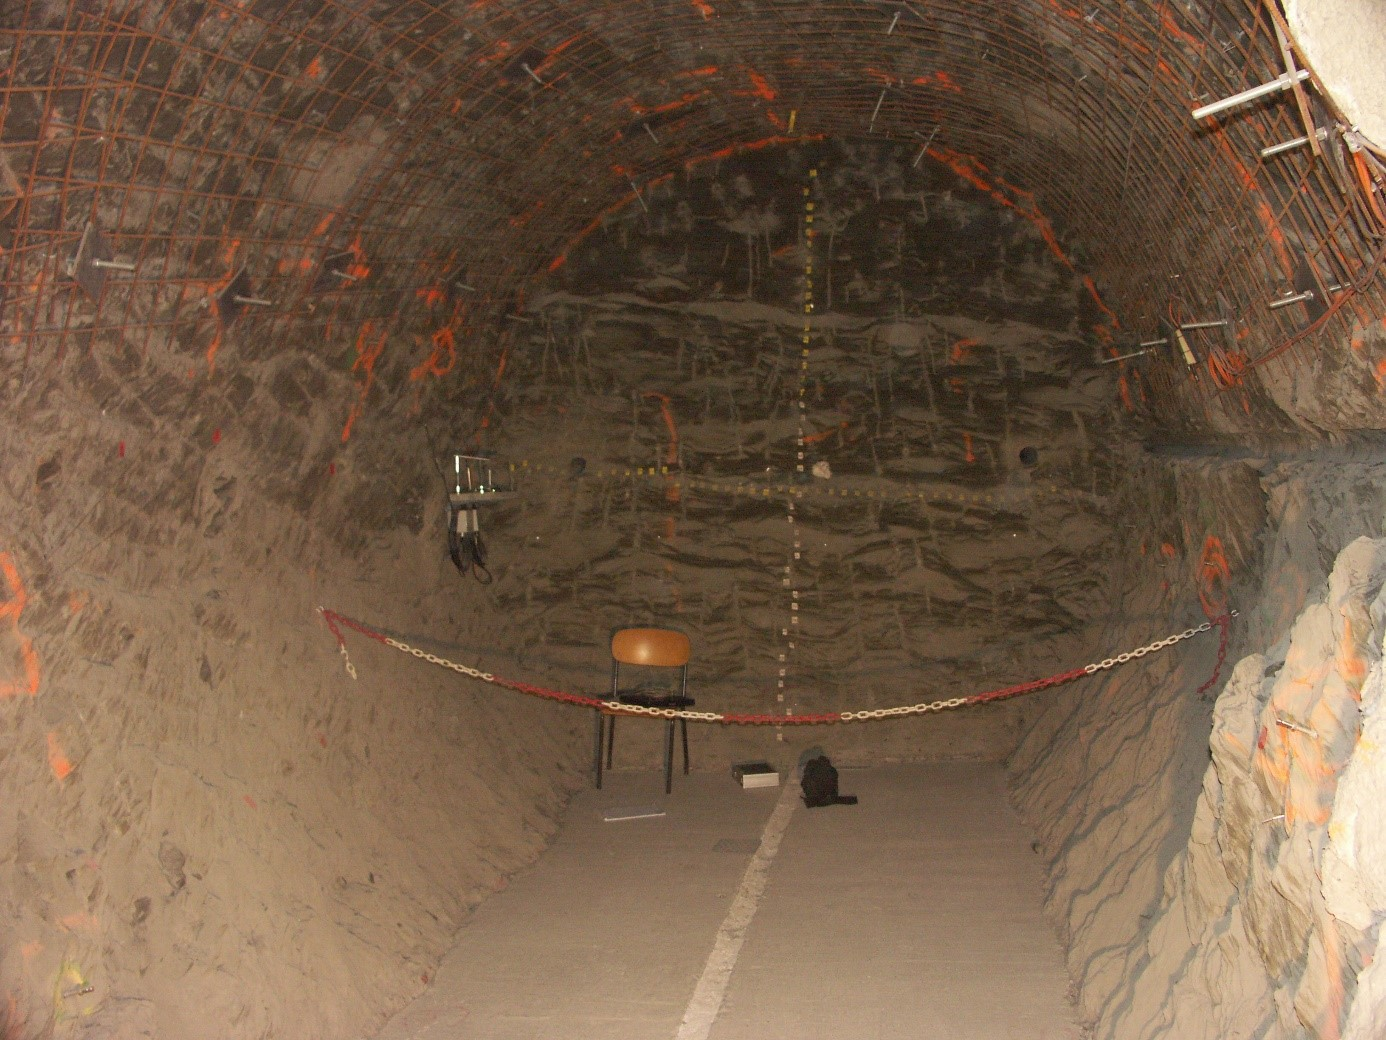
\includegraphics[width=1\textwidth]{./figures/bgr_CD_experiment.jpg}
\caption{The EZ-B niche in the Mont Terri rock laboratory, where the CD/LP experiment has been conducted since 2006 (photo: Mont Terri consortium, swisstopo).}
\label{fig:bgr_CD_experiment}
\end{figure}

A special focus of this experiment was to investigate the long-term impact of these seasonal variations on the temporal evolution of the cracks that occur during the excavation process and make up the Excavation Damaged Zone (EDZ). To this end, the EZ-B niche was excavated in the years 2004/2005 (Figure \ref{fig:bgr_CD_experiment}). Subsequently, the niche was equipped with a comprehensive set of measurement devices to record the evolution of temperature, water content, convergence of the niche and crack development at the tunnel walls over time. This measurement campaign was started in 2006 and has been continued until today to investigate long-term effects. Note that the experiment was transferred into the LP-A experiment to explicitly focus on the long-term monitoring of pore pressure. The CD/LP experiment under in-situ conditions was supplemented by laboratory experiments with drill cores to determine hydraulic-mechanical properties of the clay rock, such as porosity, grain density, etc. \cite{matray2013}. 

Characteristic macroscopic cracks on the tunnel walls have been monitored and the field data of the crack opening show a good correlation with the seasonal variation of temperature and humidity. The cyclic deformation of the crack opening yields a re-occurring compression perpendicular to the crack during summer, which typically is a time of high relative humidity and, hence, the swelling causes an increase of rock volume \cite{jaeggi2012}. This characteristic behavior of swelling and shrinking was successfully reproduced by means of hydraulic-mechanically coupled numerical simulations \cite{ziefle2018}, which provides valuable benchmark data for future investigations of the cyclic deformation of clay rock.

\subsubsection{The AD Experiment}
\index{MT-AD experiment}

The aim of the experiment is to provide core samples from the sandy facies of the Opalinus Clay as a typical example of an argillaceous host rock for the safe disposal of nuclear waste. These samples were used for experimental-numerical analysis in the framework of the GeomInt project. Additionally, a geological characterization of the cores and seismic (Interval Velocity Measurements - IVM) and geolelectrical measurements (Electrical Resistivity Tomography - ERT) in the boreholes were performed. The results of the experimental campaign yield a valuable description of the sandy facies in addition to the well characterized shaly facies of the Opalinus Clay \cite{bossart2008,jahn2016}. 
\index{ERT Electrical Resistivity Tomography}

From a geological perspective, the AD experiment gave opportunity to study the lower sandy facies of the Opalinus Clay at the Mont Terri rock laboratory in detail. The two fully cored boreholes BAD-1 and BAD-2 with a diameter of 131 mm (yielding samples of 101 mm diameter) were drilled parallel and perpendicular to the sedimentary bedding, respectively. The 15.35 m long horizontal borehole BAD-1 was drilled from 7th-10th of July 2018 by the BGR. It is located entirely in the lower sandy facies. The geological mapping was performed by swisstopo \cite{galletti2019}. The core material of BAD-1 was entirely sampled for laboratory experiments performed by the Christian-Albrechts University of Kiel (Germany) and the Institute of Geomechanics (IfG) Leipzig (Germany). The core samples were conditioned in aluminum foil and pressurized in special nitrogen-filled BGR-liners (autoclaves) to avoid further alteration. 

The BAD-2 borehole has a length of 27.0 m. It was drilled by the BGR team from 9th-17th of May 2018. The borehole is oriented perpendicular to the bedding (with a dip of 43°), thus crossing several facies types of the Opalinus Clay. The geological mapping by Swisstopo reported by Galletti \& Jaeggi (2019) \cite{galletti2019} revealed the following sequence with varying quantities of quartz, carbonates (cements and fossils) and clay minerals: 

\begin{list}{-}{\leftmargin=1em \itemindent=0em \itemsep=0em}
\item 0.0 m to 4.75 m depth: upper shaly facies,
\item 4.75 m to 19.4 m depth: lower sandy facies,
\item 19.4 m to 24.57 m depth: carbonate-rich sandy-facies, 
\item 24.57 m to 27.0 m depth: lower shaly facies.
\end{list}

This subdivision is confirmed by petrographic-structural studies and geoelectrical resistivity measurements (ERT) performed by the BGR. The BAD-2 drillcores were sampled from 4.0 m to 14.8 m (lower sandy facies) for laboratory experiments by the Universities of Kiel and IFG Leipzig. Following the procedure employed for the BAD-1 drilling, the core material was conditioned in aluminum foil and pressurized in special nitrogen-filled BGR-liners (autoclaves). The drillcore material from the intervals between 0.0 m to 4.0 m and 14.8 m to 27 m, including the transition towards the underlying carbonate-rich facies, are stored at the BGR facility in Hannover (Germany) for further geological characterization. The first results revealed a good core quality and confirm a rather uniform appearance of the sampled profile inside the lower sandy facies, the drillcore material is thus suitable for the planned experiments (cf. Figure \ref{fig:bgr_AD_experiment}).

\begin{figure}[!ht]
\centering
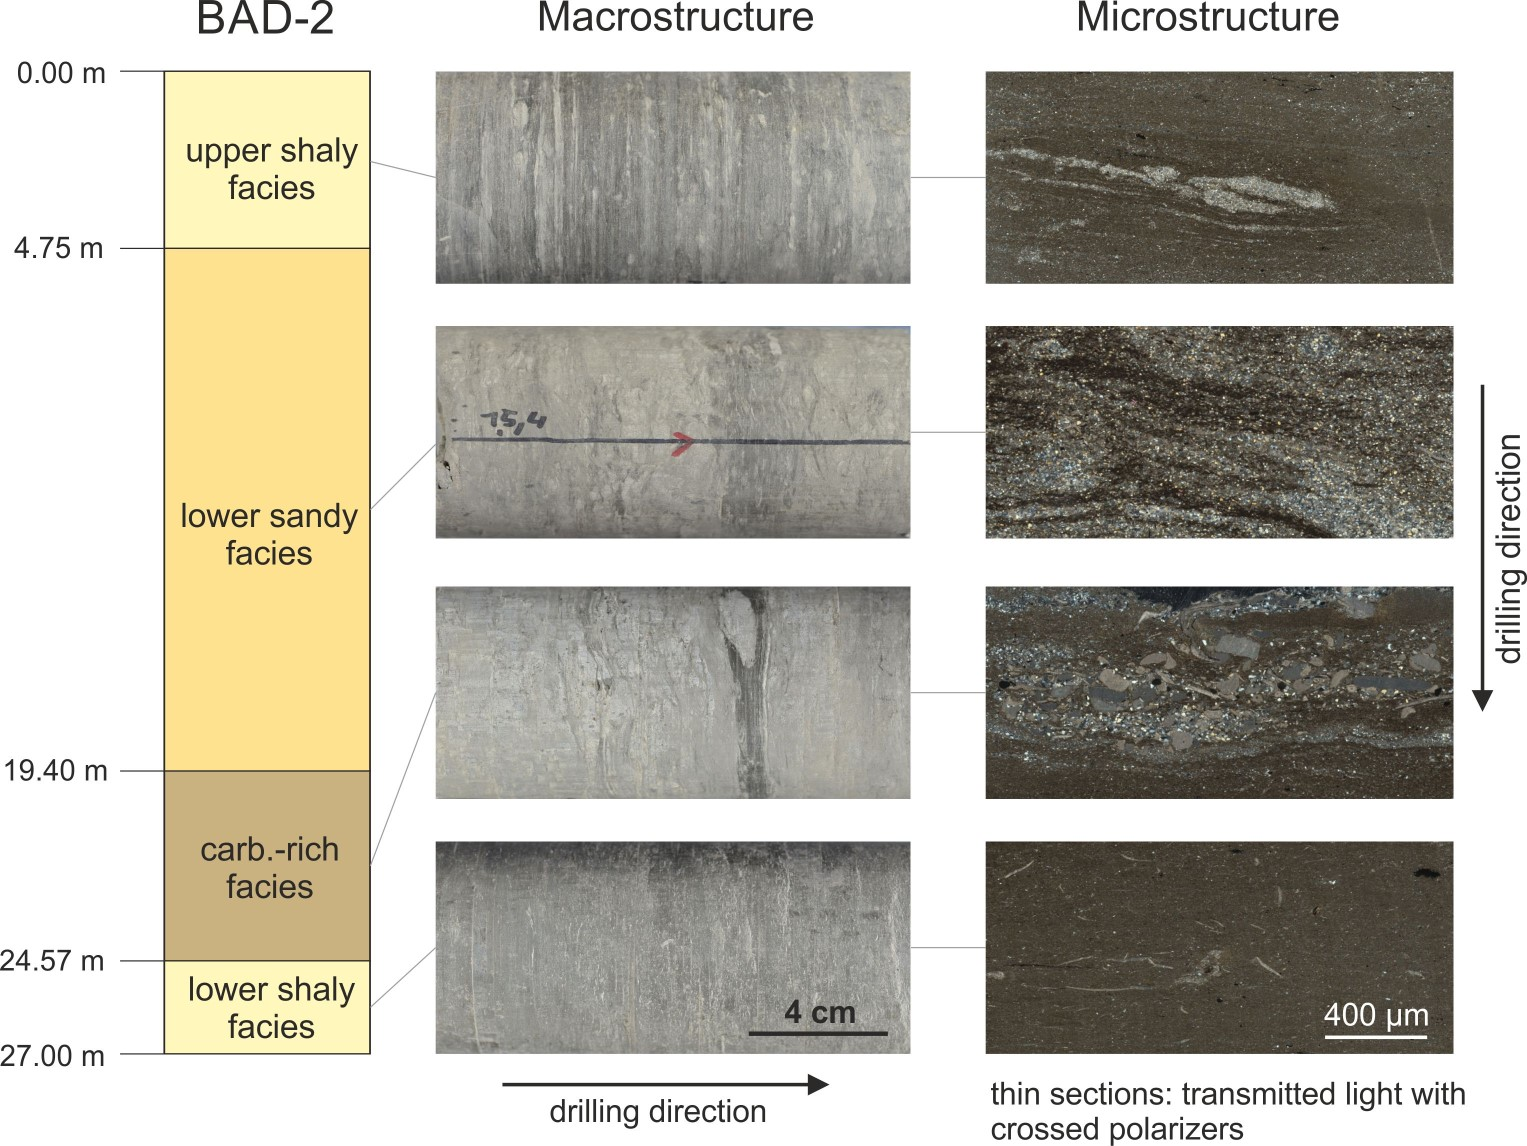
\includegraphics[width=1\textwidth]{./figures/bgr_AD_experiment.jpg}
\caption{Schematic profile of borehole BAD-2 as marked in Figure \ref{fig:bgr_mt_topview} (left), macrostructural (on drillcore scale) and microstructural features (on thin section scale) of the different facies types of Opalinus Clay encountered in the BAD-2 borehole.}
\label{fig:bgr_AD_experiment}
\end{figure}

\textbf{High resolution ERT measurements in borehole BAD-2[Markus Furche]}
\index{ERT Electrical Resistivity Tomography}
The task of geophysics was to characterise the rock unit that had been drilled through, to precisely determine the locations of the facies boundaries and to describe the variability, especially of the sandy facies. The electrical resistivity tomography (ERT) method was used for this purpose.

\textbf{Principle}
To determine the spatial electrical resistivity distribution (or its reciprocal $-$ the electrical conductivity) in the ground, a direct current (DC) is injected into the ground through two point electrodes (A, B), see Figure \ref{fig:four-electrode-array}.
\begin{figure}[!ht]
	\centering
		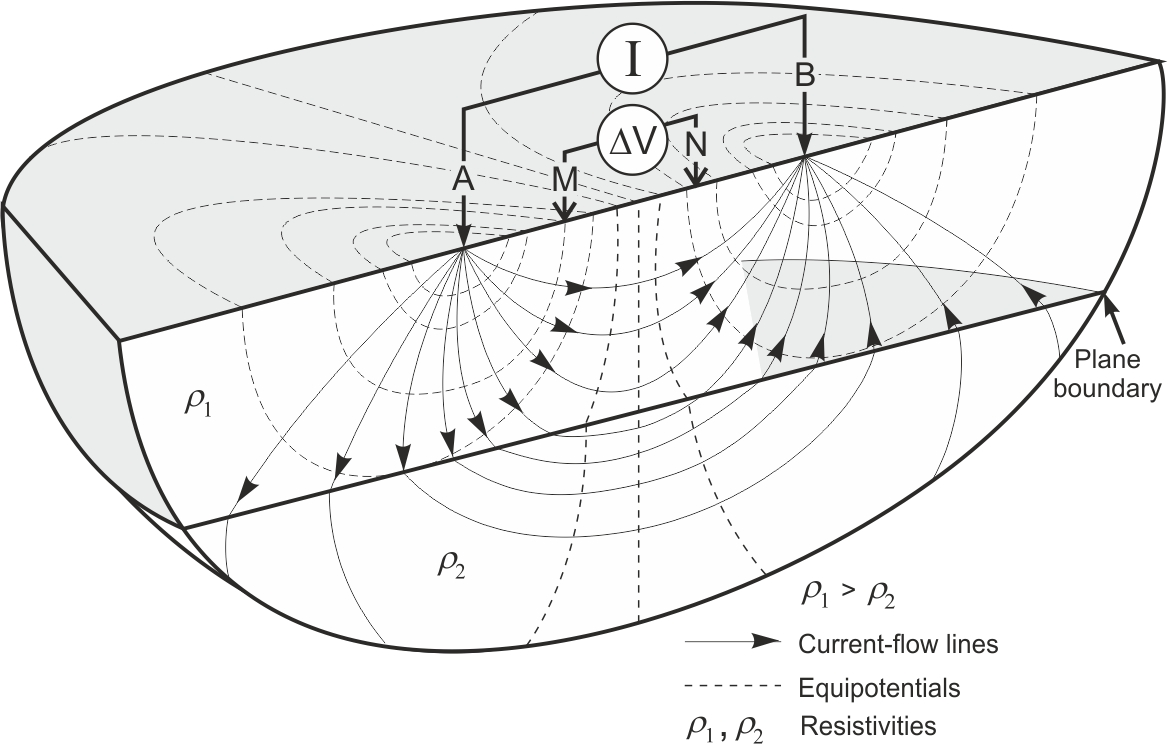
\includegraphics[width=1\textwidth]{./figures/fig-ERT-1.jpg}
	\caption{Principle of resistivity measurement with a four-electrode array (modified after Kn{\"o}del et al., 2007 \cite{knoedel2007}).}
	\label{fig:four-electrode-array}
\end{figure}
The resulting electrical field is measured using two other electrodes (M, N). A point electrode introducing an electrical current $I$ will generate a potential $V_{r}$ at a distance $r$ from the source. In the case of the four-electrode array shown in Figure \ref{fig:four-electrode-array}, the two current electrodes (A, B) introduce a current $I$. When assuming a homogeneous half-space, the potential difference $\Delta V$ between the electrodes M and N can be calculated as:
\begin{equation}
	\Delta V=\rho I \left[\frac{1}{2\pi}\left(\frac{1}{\overline{\rm{AM}}}-\frac{1}{\overline{\rm{AN}}}-\frac{1}{\overline{\rm{BM}}}+\frac{1}{\overline{\rm{BN}}}\right)\right]
\end{equation}
Here, $\overline{\rm{P}_{1}\rm{P}_{2}}$ denotes the distance between two points $\rm{P}_{1}$  and $\rm{P}_{2}$. Replacing the factor in square brackets with $1/K$ , we obtain the resistivity of the homogeneous half space as follows:
\begin{equation}
	\rho=K\frac{\Delta V}{I}.
\end{equation}
The parameter $K$ is called configuration factor or geometric factor. For inhomogeneous conditions, it yields the resistivity of an equivalent homogeneous half-space. For this value the term apparent resistivity $\rho_{a}$ is introduced, which is normally assigned to the center of the electrode array. Multi-electrode resistivity meters enable the measurement of 2D resistivity surveys (2D imaging). The advantages of this kind of measurements are their high vertical and horizontal resolution along the profile. 
An inversion process of the measured data is necessary for the final interpretation. This process transforms the apparent resistivities into a reliable model discretised into a distinct number of elements of homogeneous resistivity. All inversions are performed using the non-commercial software BERT (Boundless Electrical Resistivity Tomography \footnote{https://gitlab.com/resistivity-net/bert}) developed by Th. G{\"u}nther (Leibniz Institute of Applied Geophysics, Hannover) and C. R{\"u}cker (Technical University of Berlin).

\textbf{Measurements and Results}

\begin{figure}[!ht]
	\centering
		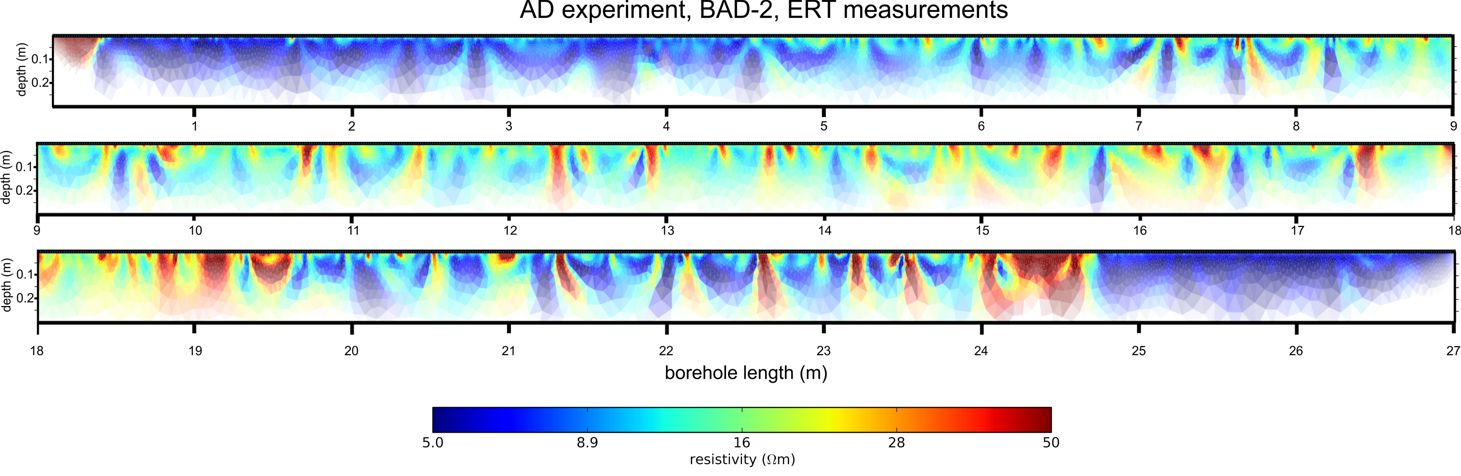
\includegraphics[width=1.35\textwidth, angle=90]{./figures/fig-ERT-2.jpg}
	\caption{Borehole BAD-2: Two-dimensional distribution of the resistivity as a result of the inversion calculation.}
	\label{fig:ERT-2d-model}
\end{figure}
The measurements were performed on May 21$^{\rm{st}}$ and 22$^{\rm{nd}}$ 2019. Since the borehole is perpendicular with respect to the bedding, measurements were only taken in one orientation (0$^{\circ}$, i.e. the electrodes are oriented upwards). Along the borehole, 35 individual profiles of 1.5 m length with half-sided overlapping were measured.

The data processing consists of the following steps: First thing is the scaling of the data in order to eliminate the geometry effects of the borehole. Then data points with high statistic error ($>3 \%$) or high phase angle (absolute value $>$ 100 mrad) were eliminated. 12 or 13 consecutive single data sets were combined to three cumulative ones (00.10 m - 09.85 m, 08.36 m - 18.10 m, 16.61 m - 26.98 m; the last record of the previous section is the first of the following). With these three data sets the inversion was performed using standard parameters. The resulting resistivity models are shown in Figure \ref{fig:ERT-2d-model}.

\begin{figure}[!ht]
	\centering
		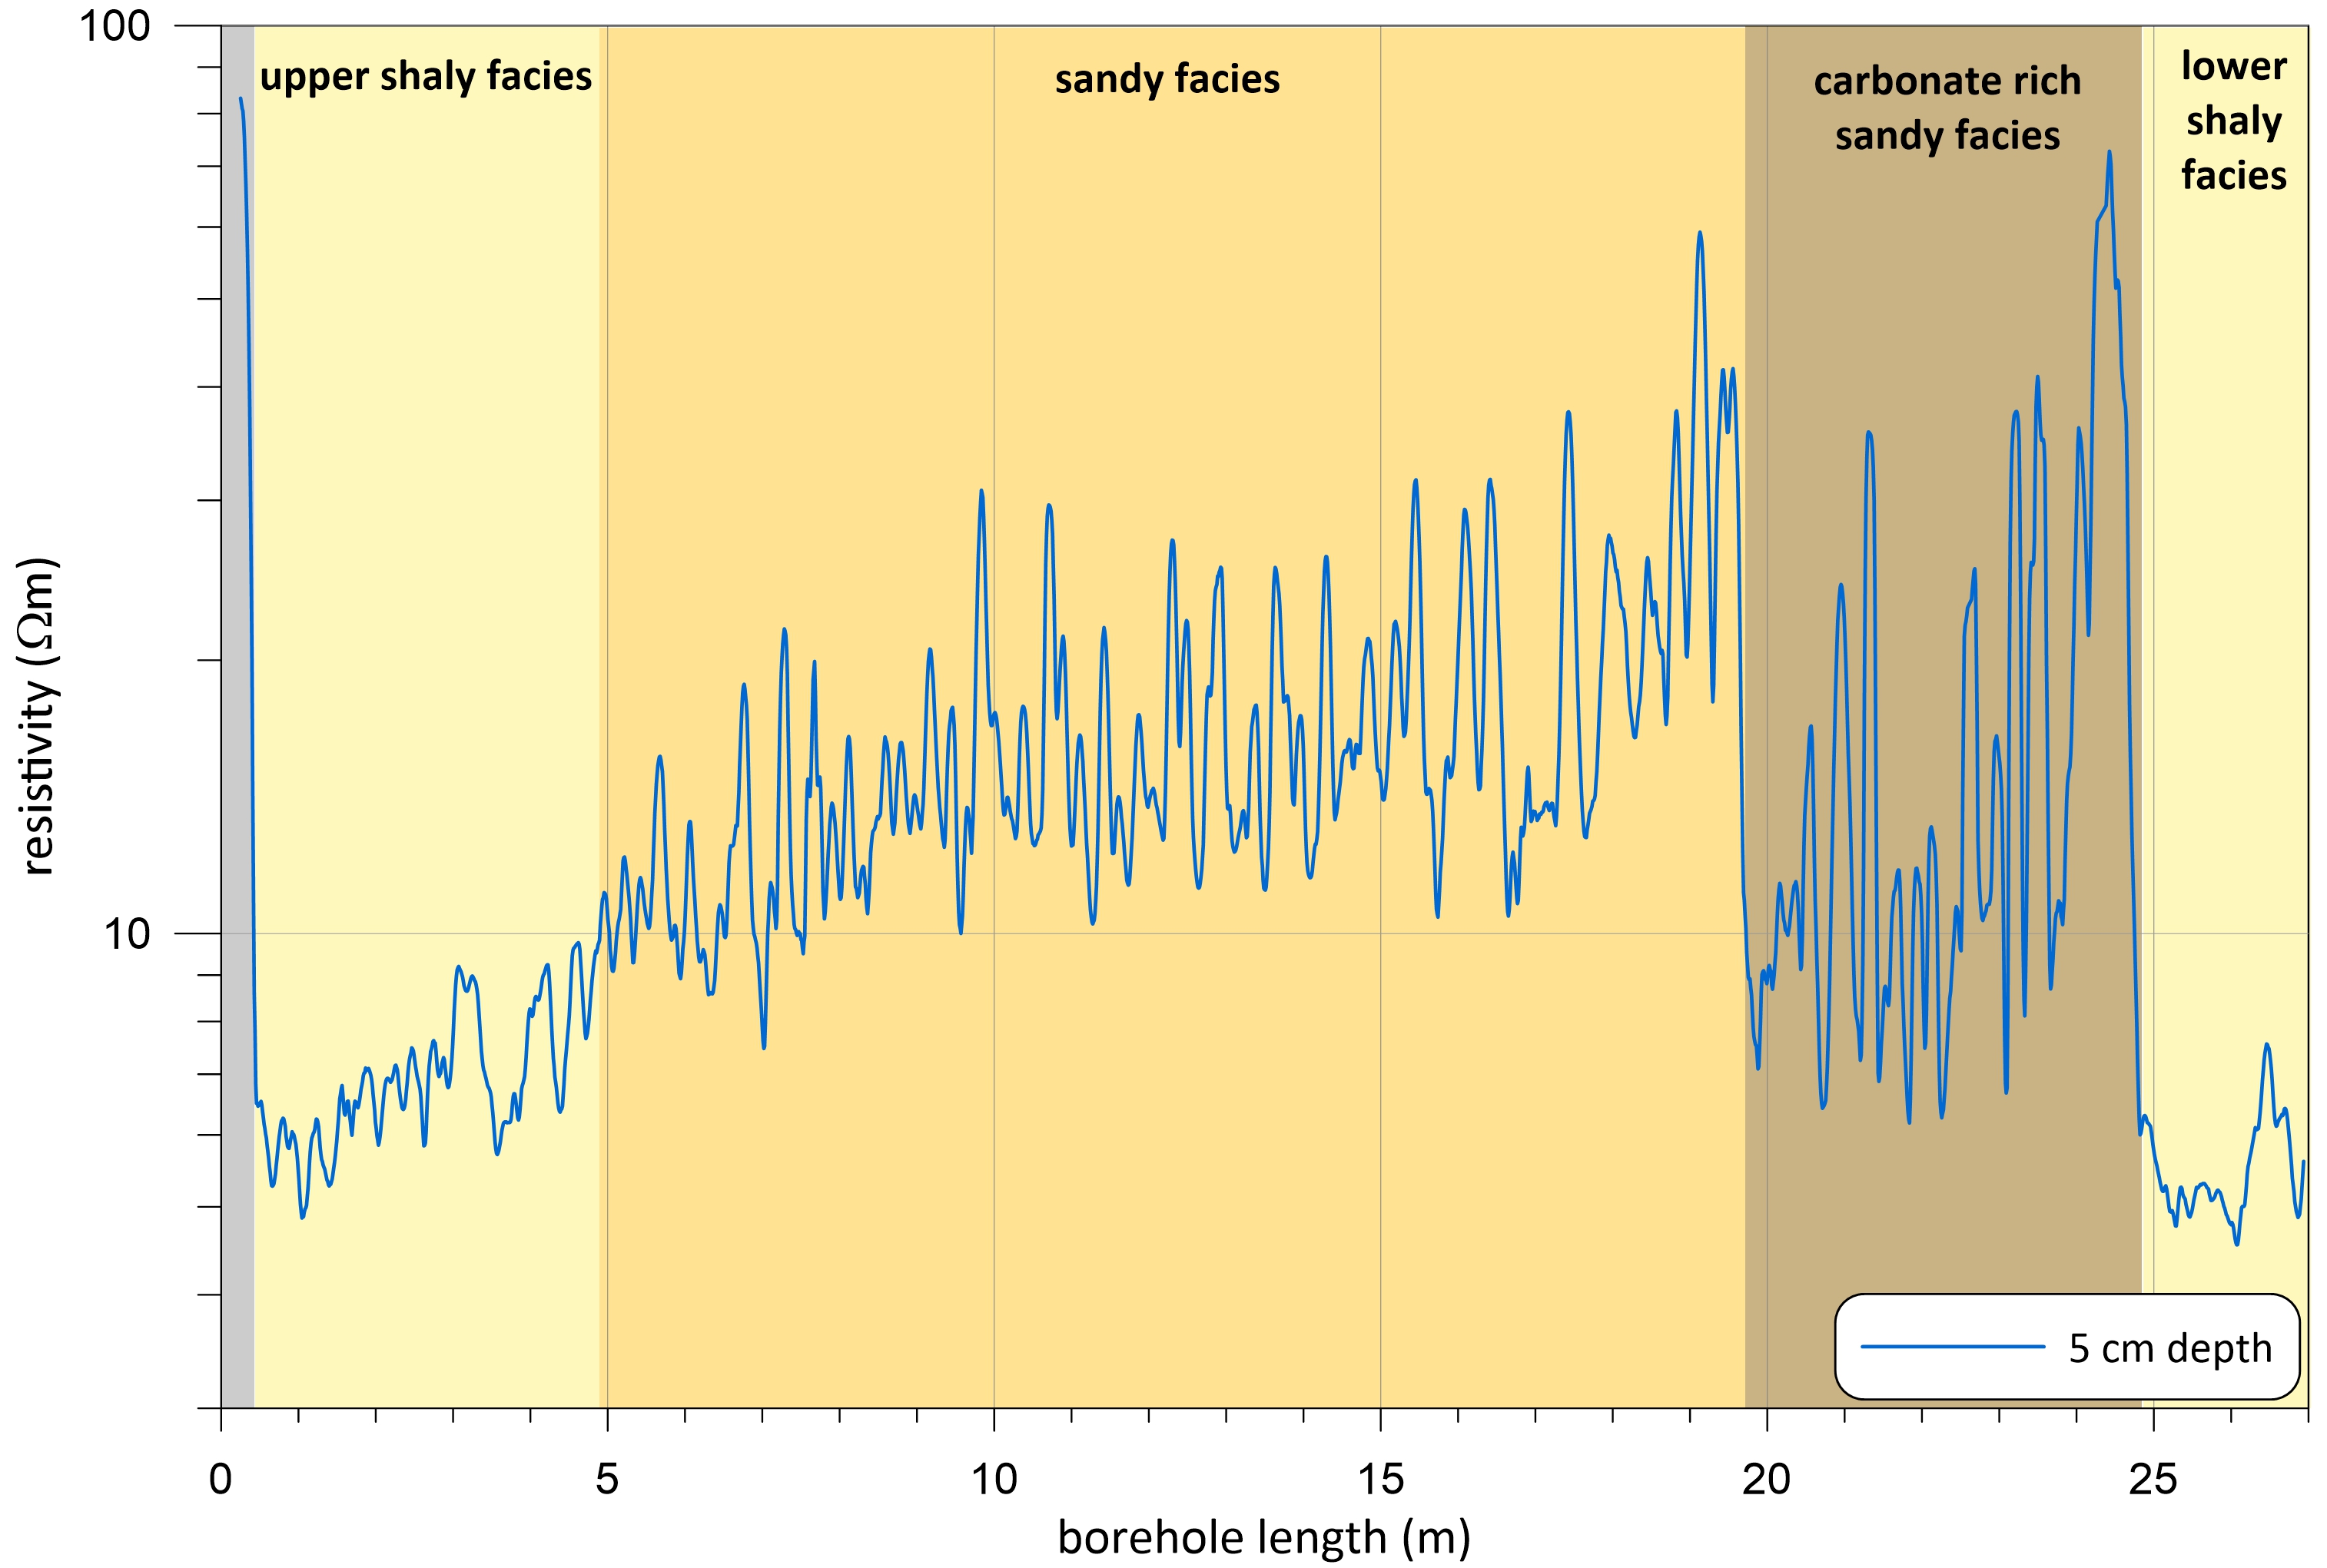
\includegraphics[width=1\textwidth]{./figures/fig-ERT-3.jpg}
	\caption{Borehole BAD-2: Curve of the resistivity at a distance of 5 cm from the borehole wall.}
	\label{fig:ERT-model-curve}
\end{figure}
Up to 50 cm borehole depth, the shotcrete can be recognised as a high-resistance structure. Beyond that, the resistivity is well below 10 $\Omega$m and rises slowly with increasing borehole depth. Embedded in this basic structure are thin layers with high resistivity ($>$ 30 $\Omega$m). Between 18.5 m and 19.5 m, there is a very extensive high-resistance range, after which the resistance level drops significantly, again with embedded high-resistance layers. Between 24.0 m and 24.7 m a second distinct high-resistance range is reached, beyond which a sharp drop to values below 10 $\Omega$m can be observed. This level is maintained down to the bottom of the borehole without further intermediate structures.

From the calculated 2D models of the resistivity, curves can be extracted for specific distances from the borehole wall. Figure \ref{fig:ERT-model-curve} shows the corresponding resistivity curve for a distance of 5 cm. The different facies types are indicated as colour background. It can be seen that both the upper and lower shaly facies are characterised by resistivities below 10 $\Omega$m with little variation. The mean level in the sandy facies (4.9 m to 19.7 m) is significantly higher (about 15 $\Omega$m), and the variability is also considerably greater. Both, the upper and the lower transition towards the carbonate-rich sandy facies are clearly indicated as a sharp drop in the resistance curve. Here, the average level of resistivity lies between the values for shaly and sandy facies, the amplitudes of the variations are highest.

\textbf{Implications of the geological-geophysical investigations}

Petrographic-structural studies form the basis for rock characterization and provide first indications for the compositional-structural variability, which independently is confirmed by geophysical borehole measurements.

ERT is able to characterise structures close to the borehole and to resolve rock variability with high accuracy. The individual facies types of Opalinus Clay can be distinguished based on mean resistivities and the type of heterogeneity (amplitudes and sequence). Especially the important transitions towards the carbonate-rich sandy facies can be precisely located.

The results confirm that the upper shaly facies is closely related to the most homogenous facies type of Opalinus Clay (the lower shaly facies). In contrast, the lower sandy facies and especially the carbonate-rich sandy facies represent the more heterogeneous endmembers of the investigated claystone formation.
The new results are consistent with published data and support the classification of the Opalinus Clay at the Mont Terri site into several major facies types. Further investigations will focus on the characterization of intra-facies variability using the sub-facies concept.




\clearpage
%---------------------------------------------------------------------------------------------------
\subsection{Rock Salt Samples}
\label{subsec:salt}
\Authors{Mathias Nest, Dirk Naumann (IfG)}

\subsubsection{The Springen in-situ laboratory}
\label{sec:springen}

The large-scale test site Merkers benefits from the unique mining situation in the bedded salt mass of the Werra salt formation (z1, Zechstein sequence) where two potash seams were mined in a room-and-pillar system at 275 m (1st floor, potash seam ''Hessen'', z1KH) and 360 m (2nd floor, potash seam ''Thüringen'', z1KTh) depth, respectively. Fig. \ref{fig:springenlab} shows the preparation of an experiment on the 2nd seam. The evaporite rocks of the Zechstein formation were laid down during the Permian period around 250 million years ago. The intact mineral deposit was locally disturbed between 14 and 25 million years ago by tertiary volcanism, leading to the mutation of some potash salts to sylvinite, and the creation of pockets of CO$_2$ under high pressure.

\begin{figure}[ht!]
\centering
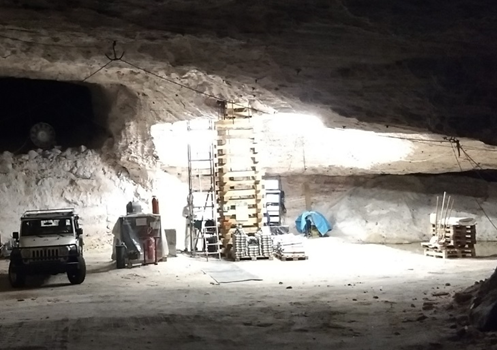
\includegraphics[width=0.85\textwidth]{figures/springen2ndseam.png}
\caption{Preparation of experiments on the second seam.}
\label{fig:springenlab}
\end{figure}

The pressurized tests are conducted between the two potash seams in the very homogeneous Middle Werra rocksalt (z1Na). It consists mostly of very pure halite layers intersected by thin anhydrite lines or bands of rocksalt with finely distributed anhydrite accessories indicating the sedimentary bedding. 

Because the test results depend mainly on the acting stress field, i.e. the minimal stress distribution in the rock mass around the test area, it has been measured and  characterized by hydro-frac measurements, and is thus well-known. The minimal stresses in the contour increase with progressive distances from the underground openings until reaching a constant value in a depth of around 15 m. The measured value of an undisturbed stress state of around 8 MPa corresponds fairly well to calculated lithostatic stresses of 7.8 to 8.8 MPa. 

The main facility is a large borehole of nearly vertical 60 m height and 1.3 m diameter. It was drilled upwards from the second floor, ending about 20 m beneath the first floor. For access to the later sealed volume an 85 mm pilot hole has been drilled from the upper floor. The borehole was closed by a 20 m high MgO-concrete plug. 

For monitoring of micro-seismic events, e.g. due to creation of an excavated damage zone around underground openings or fluid flow driven damage, a highly sensitive AE-network was installed in observation boreholes, which were drilled parallel to the main borehole. This network has constantly been updated and extended over the past years. Signals of magnitude M $<$ -4 can be detected in a frequency range from 1 kHz to 200 kHz. This corresponds to intergranular microcracking on grain boundaries on a millimeter- to centimeter-scale. 

\subsubsection{Rock salt laboratory}

The following conditions and equipment are available in the IfG labs for rock mechanical laboratory investigations:

\begin{list}{-}{\leftmargin=1em \itemindent=0em \itemsep=0.1em}
\item Climate-controlled rooms for storage of specimens at conditions which correspond to those present in situ
\item Laboratory for mineral-petrographic examinations, density and moisture determination, ultra-sound measurements and 
photographic documentation
\item Workshop for the preparation of specimens in high precision according to testing requirements (rock saws, lathes etc.)
\item Test laboratory containing various servo-controlled hydraulic testing machines for conducting investigations on 
rock mechanics in accordance with the up-to-date state of research and development (see Figure \ref{fig:ifglabph1}).
\end{list} 

\begin{figure}[!ht]
\centering
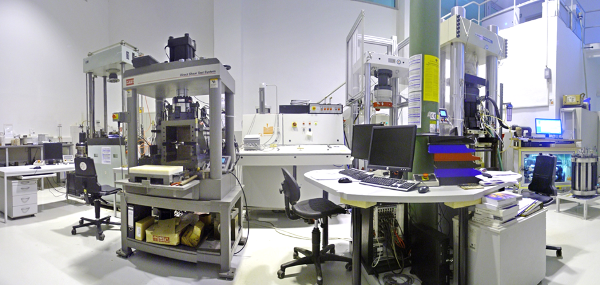
\includegraphics[width=1\textwidth]{./figures/ifg-lab-photo1-v2.png}
\caption{View inside the rock mechanical lab with various servo-controlled hydraulic testing machines.}
\label{fig:ifglabph1}
\end{figure}

It has to be mentioned that some of the applied IfG test procedures have been developed for the requirements of the specific IfG-material laws. 
But generally they are in accordance to ASTM and ISRM standards resp. equivalent descriptions, e.g.:

\begin{list}{-}{\leftmargin=1em \itemindent=0em \itemsep=0.1em}
\item ASTM D 4543-85 Standard Practice for Preparing Rock Core Specimens and Determining Dimensional and Shape Tolerances
\item ASTM D 2845-05 Standard Test Method for Laboratory Determination of Pulse Velocities and Ultrasonic Elastic Constants of Rock
\item ASTM D 2664-86 Standard Test for Triaxial Compressive Strength of Un\-drained Rock Core Specimens without Pore Pressure Measurements 
\item DGEG (1979):   Empfehlung Nr. 2 des AK 19 der DGEG (Dreiaxiale Druckversuche).
\item ASTM D4406-04 Standard Test Method for Creep of Cylindrical Rock Core Specimens in Triaxial Compression
\item ASTM D7070-04 Standard Test Method for Creep of Rock Core Under Constant Stress and Temperature
\item ISRM: Suggested Methods for Determining o the Uniaxial Compressive Strength and Deformability of Rock Materials
\item ISRM: Suggested Methods : Part 2 : 2007 - Unconfined Compressive Strength with Young's Modulus and Poisson's Ratio
\item ISRM: - Suggested Methods : Part 2 : Received 1983 - Strength of Rock Material in Triaxial Compression
\end{list}

\subsubsection{Sample characterization and pre-investigation}

Several preliminary investigations are usually done before lab testing. After preparing the cylindric samples (cutting with a rock saw and smoothing the samples with a lathe) in the IfG labs, their density is determined by measuring the geometrical dimensions and the mass. Concerning the quality of these parameters an accuracy in length determination is $<$ 0.01 mm, those in mass determination is $<$ 0.01 g. 

Additionally, ultrasonic investigations are carried out to check integrity, homogeneity and isotropy of the samples. The ultrasonic pulse measurement system used for transmission of the rock specimens consists of two transducer sets for P-waves and S-waves and a receiver system for generating and evaluating the ultrasonic signals. The specimen is placed in physical contact between two piezoelectric transducers, one acts as a driver and the other one acts as a receiver. The transit time of the mechanical pulse to pass through the specimen is used to determine elastic wave velocity.

For samples where both P- and S-waves were measured in axial sample direction the elastic constants are obtained from density ($\rho$) and the ultrasonic velocities ($v_p$, $v_s$) using the following expressions derived from the theory of elasticity for homogeneous, isotropic solids:

\begin{equation}
\label{eq:YoungsModulus_Ultrasonic}
E_{dyn} = \frac{\rho v_s^2(3v_p^2-4v_s^2)}{v_p^2-v_s^2} 
\end{equation}
\begin{equation}
\label{eq:PoissonsRatio_Ultrasonic}
\nu_{dyn} = \frac{v_p^2-2v_s^2}{2(v_p^2-v_s^2)}
\end{equation}

Dynamic elastic parameters of the various rock portions determined on the base of sonic wave velocity at room temperature are in a wide range representing typical values for the various materials as known from other locations. 


\clearpage
%---------------------------------------------------------------------------------------------------
\subsection{Crystalline Rock Samples}
\label{subsec:crystalline}
\Authors{TU Freiberg}

\subsubsection{URL Reiche Zeche Freiberg}\index{URL Reiche Zeche}

\todod{[TUBAF](): Noch eine Abbildung zur Reiche Zeche?}

\begin{wrapfigure}{l}{6cm}
\centering
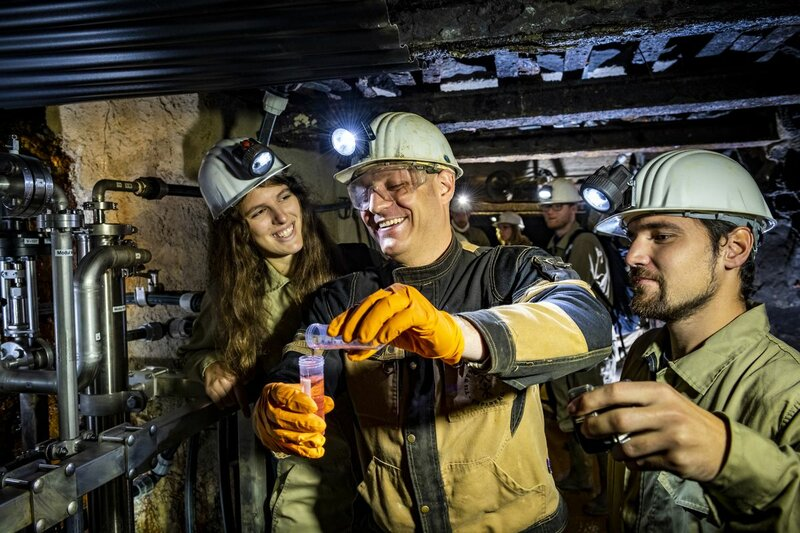
\includegraphics[width=5.9cm]{figures/reiche-zeche.jpg}
\caption{The Reiche Zeche in Freiberg, \cite{ReicheZechePicture}.}
\end{wrapfigure}
The Reiche Zeche mine is located north-east the city center of Freiberg, Saxony. It operated as a silver mine for several centuries. It became a part of the TU Freiberg 1919 when silver mining definitely was no longer profitable. Nowadays the mine is used as an underground research laboratory (URL) and for teaching purposes. The roughly $4\,\text{km}^2$ sized area is well documented in terms of geology, mineralogy, geophysics and geometry. Draining of the mine is done using the "Rothsch\"onberger Stollen (tunnel)". A detailed overview about the history of the Reiche Zeche can be found in \cite{ReicheZecheHistory}.

Due to its long history, the development of new technologies and the importance for the development of the whole region the mining sites and the associated infrastructure are listed as UNESCO world heritage site since 2019.

Current projects are for example dealing with bio-leaching or complex experiments which study the influence of hydro-fracking experiments on the stress state (STIMTEC project).

The Reiche Zeche is equipped with an underground railway system, installed electricity, water and air pressure. The experienced staff and the nearby located mining agency help to successfully conduct experiments in about 150 m depth. 

\clearpage
\subsubsection{Rock material used in the direct shear tests}

\begin{figure}
\begin{subfigure}[c]{0.5\textwidth}
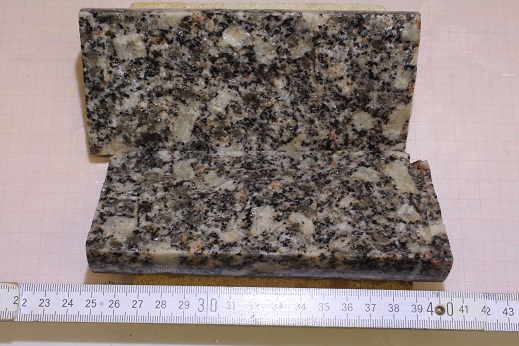
\includegraphics[width=0.99\textwidth]{./figures/ExpRockGranite.JPG}
\subcaption{Granite sample}
\label{fig:RockGranite}
\end{subfigure}
\begin{subfigure}[c]{0.5\textwidth}
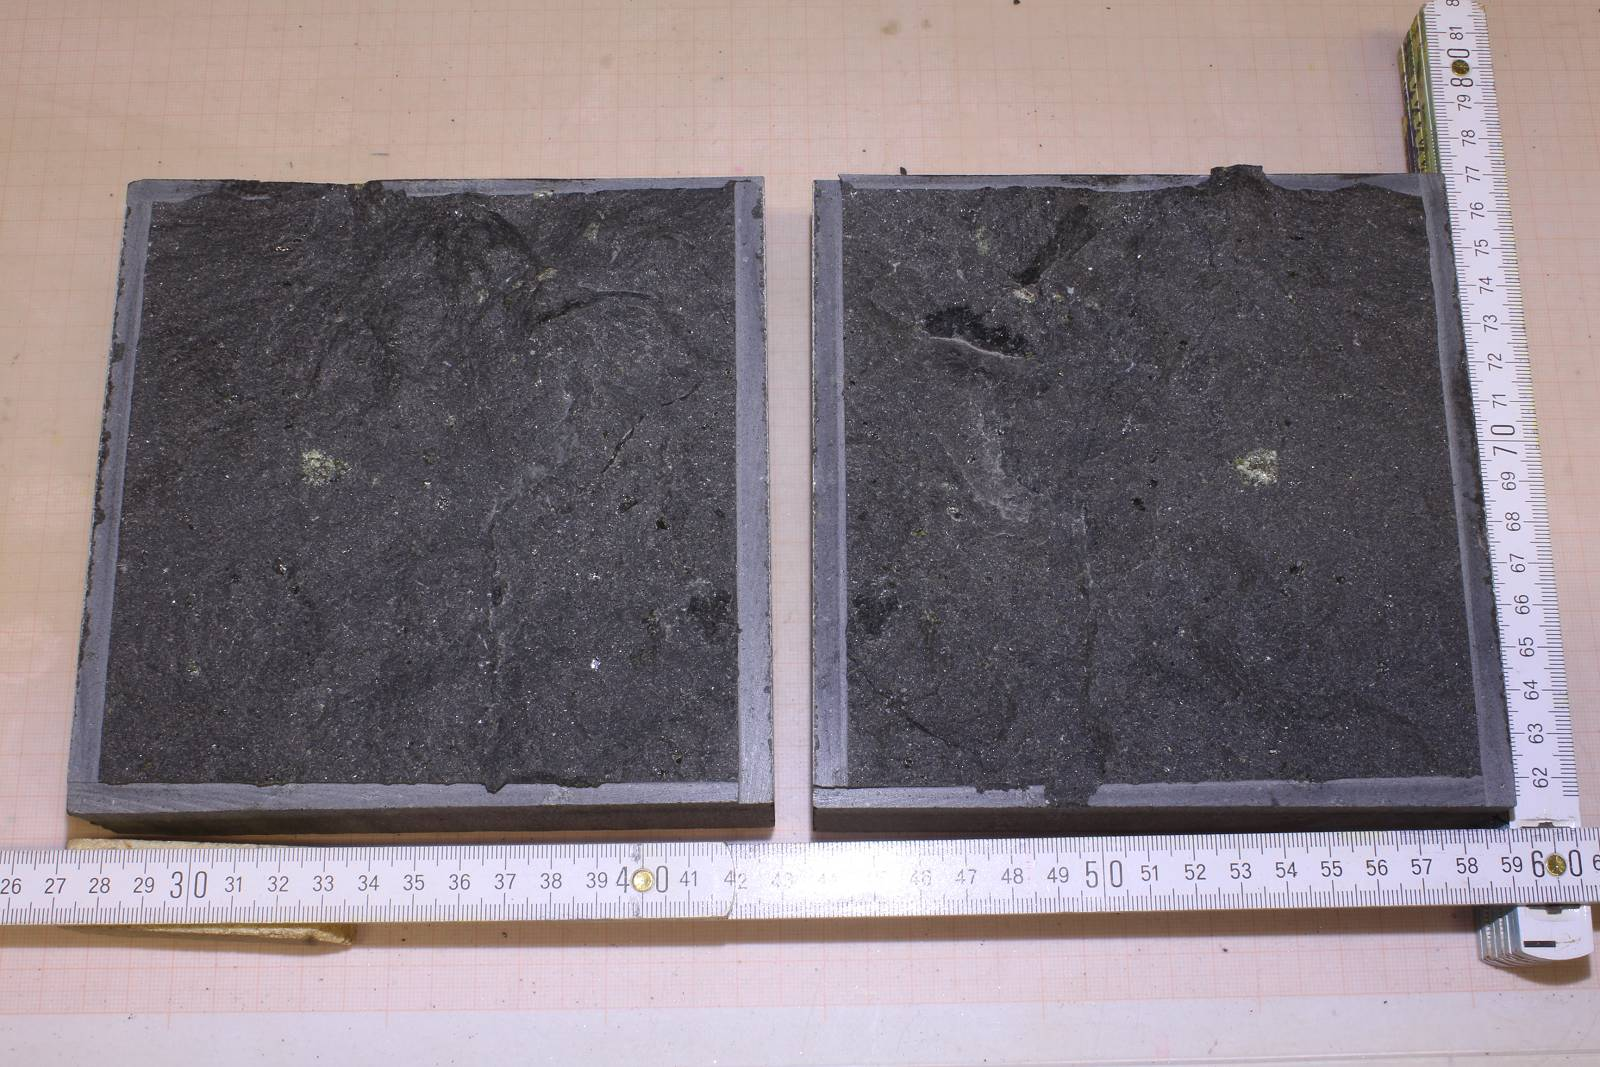
\includegraphics[width=0.99\textwidth]{./figures/ExpRockBasalt.jpg}
\subcaption{Basalt sample}
\label{fig:RockBasalt}
\end{subfigure}
\caption{Crystalline rock samples under investigation}
\end{figure}

Two different crystalline rock \index{crystalline rock} types are used. Granite is a coarse-grained intrusive igneous rock. The grains are on the millimetre to centimetre scale, see Fig. \ref{fig:RockGranite}. The typical main minerals of granites are quartz, feldspar and plagioclase. The used granite origins from Kirchberg, Saxony.
%
Basalt is an fine-grained extrusive igneous rock. It is rich of plagioclase. See Fig. \ref{fig:RockBasalt}. Its origin is V\"olkershausen, Thuringia.
%
Lab tests to evaluate basic rock parameters of the intact rock material have been conducted. The values of the granite and basalt used in the experiments can be found in Tab. \ref{table:MEX7_rockParam}.

\begin{table}[!ht]
\begin{center}
\begin{tabular}{l c r r r}
variable & symbol & granite & basalt & unit\\
\hline
density & $\rho$ & $2.59$ &3.06 &$\text{g}/\text{cm}^3$\\
compressive strength & $\sigma_c$ & $120.54$&272.92 &$\text{MPa}   $\\
tensile strength & $\sigma_t$ & $7.02$&16.61 &$ \text{MPa}   $\\
%static elastic modulus & $E_s$ & $50.00$& &$ \text{GPa}   $\\
elastic modulus & $E$ & $49.75$&105.46 &$ \text{GPa}   $\\
Poisson's ratio & $\nu$ & 0.26 & 0.26  & -\\
fracture toughness & $K_I$ & $0.95$& 2.61 &$\text{MPa}\cdot\text{m}^{0.5}$\\
friction angle (Mohr) & $\Phi$ &  $52.5$& 44 &$^\circ$\\
cohesion & $c$ &  $22.5$& 25.00  &$ \text{MPa}   $\\
basic friction angle &$\varphi_b$ &30 & 31.2 & $^\circ$\\
\end{tabular}
\caption{Rock parameters of granite and basalt used in the direct shear tests.}
\label{table:MEX7_rockParam}
\end{center}
\end{table}

The elastic modulus and the compressive strength were determined using uni-axial compression tests. For the tensile strength a tension test was conducted and the fracture toughness is evaluated by a bending test. The cohesion was determined through a shear test using a saw-cut joint. Ultrasonic measurements were used to determine the Poisson's ratio.
%
The basic friction angles were determined based on \cite{Alejano20121023}. The inner friction angle of basalt is from \cite{Schultz19951} and of granite from \cite{Lanaro2005} and \cite{Ramana2019273}.

\subsubsection{Rock Surface Scanning}
\todo[inline]{[TUBAF](): What about the rock surface scanning? for section \ref{sec:material-properties} ?}
Important measurements to characterise a rock surface are surface scans. In the laboratory of the TU Freiberg a white light scanner is used, see Fig. \ref{TUBAFScanner}. It is a non-contact method which uses monochromatic light. A fringe projection is done and surface scans of rock samples with a resolution of about $30-50 \unit{\mu m}$ can be calculated. Further details about the scanning device can be found in \cite{TUBAFScanningDevice}. 

\begin{figure}[!ht]
\centering
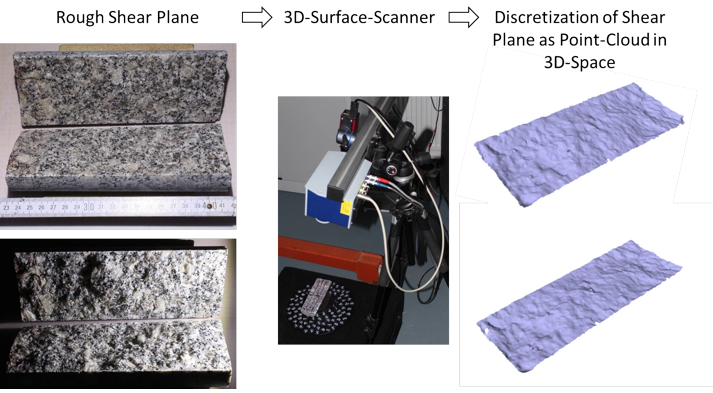
\includegraphics[width=0.95\textwidth]{figures/geomint-wp3-12a}
\caption{Surface scanning. A rock surface is digitized using a surface scanning device. The result is a point cloud.}\label{TUBAFScanner}
\end{figure}
\clearpage
%---------------------------------------------------------------------------------------------------
%===================================================================================================
\section{Thermo-Hydro-Mechanical Laboratory Tests}
\label{sec:thm-lab-tests}
In this section basic methods for rock characterization are briefly introduced such as 
characterization of rock structure (sec. \ref{subsec:structure}),
fracture toughness as materials resistance to fracture propagation (sec. \ref{sec:Fracture_Toughness_Exp}),
Brazilian tests to determine split tensile strength (sec. \ref{sec:Brazilian_Disk_Exp},
and triaxial tests to investigate the three-dimensional strain-strength behavior (sec. \ref{sec:True_Triaxial_Exp}).
%---------------------------------------------------------------------------------------------------
\subsection{X-ray Micro Computed Tomography}
\label{subsec:structure}
\Authors{Matthias Ruf (UoS)}
\index{XRCT X-ray Micro Computed Tomography}

X-ray micro computed tomography ({\textmu}XRCT) is a non-destructive imaging technique and provides the possibility to examine the inner structure of an object by creating a digital 3D image of the same. It is based on the mathematical combination, called reconstruction, of several radiograms which were acquired from different directions. Thereby, a radiogram represents the respective measured intensity values $I(L)$ of the X-rays at position $x = L$ after travelling through the object and can be related to the unattenuated X-rays intensity $I_0$ before the object at position $x = 0$ by the Beer-Lambert law. Under the assumption of a monochromatic X-ray beam this can be written as 

\begin{align*}
I(L) = I_0 \exp\left(-\int_0^L \mu(x) \mathrm{d}x \right)
\end{align*}

for an inhomogeneous material with the unknown material depending attenuation coefficients $\mu(x)$ which are determined during the reconstruction process, cf. \cite{Carmignato2018}.
\index{Beer-Lambert law}

In Figure~\ref{fig:CTsystem} the self-made open and modular {\textmu}XRCT system at the Institute of Applied Mechanics - Chair of Continuum Mechanics of the University of Stuttgart, see \cite{Ruf2020} is depicted. 

\begin{figure*}[ht]
\centering
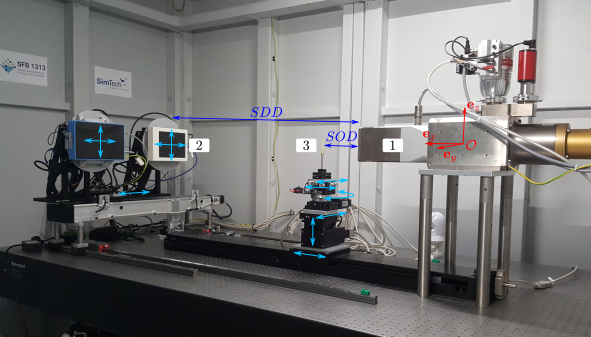
\includegraphics[width=1.0\textwidth]{figures/exp_2_2_xray_main.png}
\caption{Overview of the {\textmu}XRCT-system. The light blue arrows show the possible moving directions of the motorized stages.}
\label{fig:CTsystem}
\end{figure*}

It consists of the three main components: The X-ray source (1), the X-ray detector (2) and the sample positioning system including the rotation stage in between (3). Like most industrial CT-systems the specimen is rotated during the scan and the remaining parts are fixed. The employed X-ray tube provides a maximum power up to \SI{80}{\watt} and at the same time a focal spot size down to \SI{3}{\micro\meter} for moderate power levels. The acceleration voltage of the tube can be adjusted in the range of \SI{30}{\kilo\volt} to \SI{180}{\kilo\volt} and the flux from \SI{10}{\micro\ampere} to \SI{1000}{\micro\ampere}. It can be chosen between two indirect conversion flat panel detectors with different characteristics and resolutions of $1944 \times 1536$ and $2940 \times 2304$ pixels. Both produce gray value images with a pixel depth of \SI{14}{bit} and each is separately mounted on high accurate, motorized XY stages. The latter offers the possibility to compensate for bad detector pixels by taking several images from slightly different detector positions and subsequently stitching of the same to improve the final image quality.

The geometric magnification $M$ is given by the relation of the source detector distance $SDD$ to the source object distance $SOD$, $M = SOD/SDD$, and can be adjusted in a wide range. Depending on the sample material and the smallest feature size of interest, the specimen's diameter can be up to \SI{100}{\milli\meter}. The maximum achievable spatial resolution of the system is about \SI{50}{lp/mm} at \SI{10}{\%} of the modulation transfer function (MTF) which means a smallest feature size of \SI{10}{\micro\meter} that can be resolved. The corresponding field of view for this case is \SI{5.88}{\milli\meter} in width and \SI{4.60}{\milli\meter} in height. Therefore, the smallest expedient sample diameter is about \SI{5}{\milli\meter}. The open and modular concept of the CT-system provides a broad range also for unconventional investigations.

In Figure~\ref{fig:exampleCarraraMarble} a CT scan of a cylindrical Carrara marble core with a diameter of \SI{5}{\milli\meter} for a high resolution scan is shown exemplarily.
\begin{figure*}[ht]
	\centering
    \begin{subfigure}[c]{0.49\textwidth}
    \centering
	\label{fig:exampleCarraraMarble3D}
	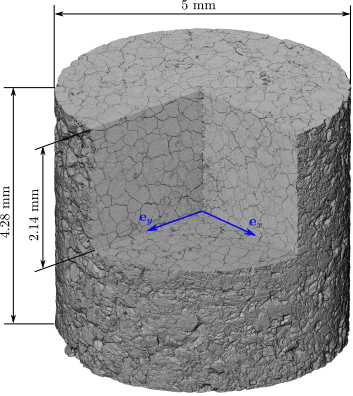
\includegraphics[width=0.9\textwidth]{figures/exp_2_2_scan_3d.png}
    \end{subfigure}
    \begin{subfigure}[c]{0.49\textwidth}
    \label{fig:exampleCarraraMarble2D}
	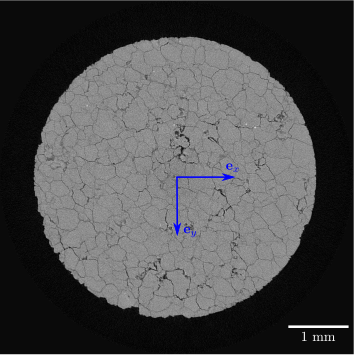
\includegraphics[width=0.9\textwidth]{figures/exp_2_2_scan_2d.png}
\end{subfigure}
\caption{CT scan of a Carrara marble core after thermal treatment.}
\label{fig:exampleCarraraMarble}
\end{figure*}

The visible micro-cracks along the grain boundaries were created by thermal treatment and are not present in the virgin state.  The geometric magnification was set to $M = 24.76$ which corresponds to the highest achievable spatial resolution and leads to a voxel size of \SI{2}{\micro\meter}. For additional details see \cite{Ruf2020}. Besides a qualitative assessment, the data sets offer the possibility of deriving several additional information by image processing. For instance, in geosciences the 3D pore characterization, the 3D grain analysis and the fracture analysis, cf. \cite{Cnudde2013}. 
%---------------------------------------------------------------------------------------------------
%% -----------------Fracture toughness (CAU Kiel)
\subsection{Fracture Toughness of the Opalinus Claystone}
\label{sec:Fracture_Toughness_Exp}
\Authors{CAU Kiel}

In linear elastic fracture mechanics, a materials resistance to fracture propagation is known as fracture toughness. The unit of the fracture toughness is $Pa.\sqrt m$ and the fracture toughness is measured under coupled or individual three different fracture modes I, II and III. In a three-point bending test, the flexural strength ($\sigma_{flex}$), flexural Young's modulus ($E_{flex}$) and flexural strain ($\epsilon_{flex}$) parameters are measured. The fracture toughness test using the three-point bending test provides the Mode I fracture toughness ($K_{Ic}$) of the material (Fig.  \ref{fig:Amir_Fracture_Toughness_Theory}).
\index{fracture toughness}
\index{three-point bending test}

\begin{figure}[!ht]
\centering
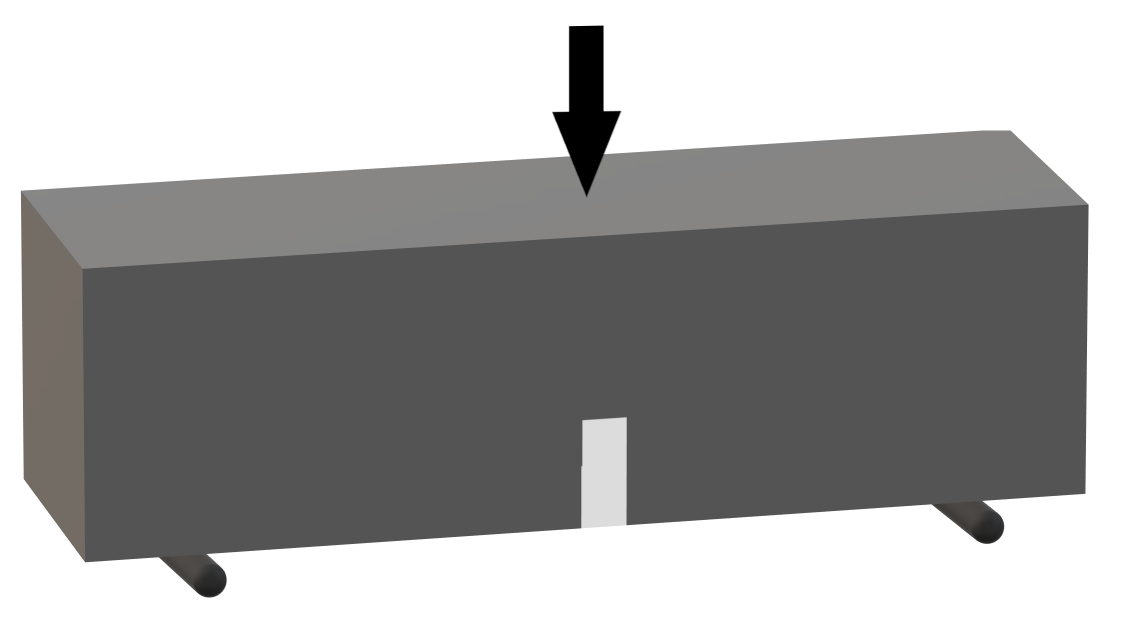
\includegraphics[width=6cm,height=3cm]{figures/Amir_Fracture_Toughness_Theory.png}
\caption{The fracture toughness assessment using three-point bending test}
\label{fig:Amir_Fracture_Toughness_Theory}
\end{figure} 

The stress intensity factor ($K_I$) on the crack tip of predefined notch is obtained with equation (\ref{eq:Fracture_Toughness}) \cite{Bower2009},

\begin{multline}
\label{eq:Fracture_Toughness}
K_I=
\frac{4f_{flex}}{B_{flex}}
\sqrt{\frac{\pi}{W_{flex}}}
\left(1.6
\left(\frac{a_{flex}}{W_{flex}}\right)^\frac{1}{2}
-
2.6\left(\frac{a_{flex}}{W_{flex}}\right)^\frac{3}{2} 
\right.
\\ 
\left.
+12.3\left(\frac{a_{flex}}{W_{flex}}\right)^\frac{5}{2} -21.2\left(\frac{a_{flex}}{W_{flex}}\right)^\frac{7}{2}
+21.8\left(\frac{a_{flex}}{W_{flex}}\right)^\frac{9}{2}
\right)
\end{multline}

where, $f_{flex}$ is the flexural load, $a_{flex}$ is the length of the pre-defined notch, $B_{flex}$ and $W_{flex}$ are the thickness and height of the sample under the flexural test, respectively. During the test procedure, the load and crack mouth opening displacement (CMOD) values are measured and plotted. At the load in which the crack starts to propagate into the medium the fracture toughness $K_{Ic}$ is calculated. In order to perform the fracture toughness test, a loading cell with three rolling supports is required (Fig. \ref{fig:Amir_Fracture_Toughness_Setup_a}). However, the in-situ condition can only be reached when a material is under controlled temperature and humidity conditions. Therefore, a climate chamber in a laboratory of CAU Kiel has been utilized to reach the desired temperature and humidity (Fig. \ref{fig:Amir_Fracture_Toughness_Setup_b}). The temperature can be controlled between 20 to 80 $^{\circ}C$ and relative humidity varies from 0 up to 100. 
\index{crack mouth opening displacement (CMOD)}

\begin{figure}[!ht]
\centering
\begin{subfigure}[c]{0.6\textwidth}
\centering
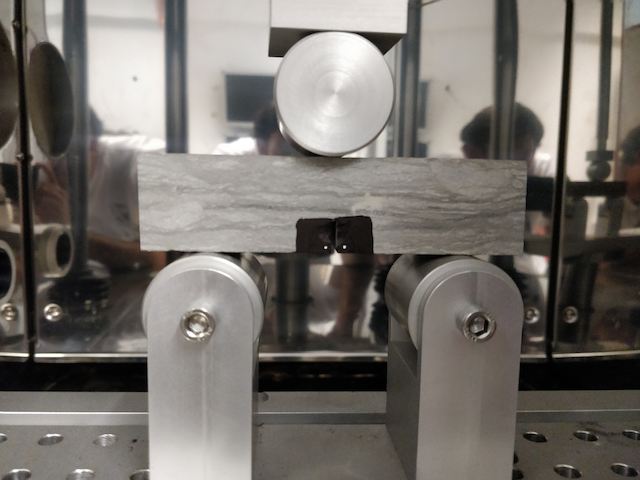
\includegraphics[width=6cm,height=5cm]{figures/Amir_Fracture_Toughness_Setup_a.png}
\subcaption{}
\label{fig:Amir_Fracture_Toughness_Setup_a}
\end{subfigure}
\begin{subfigure}[c]{0.38\textwidth}
\centering
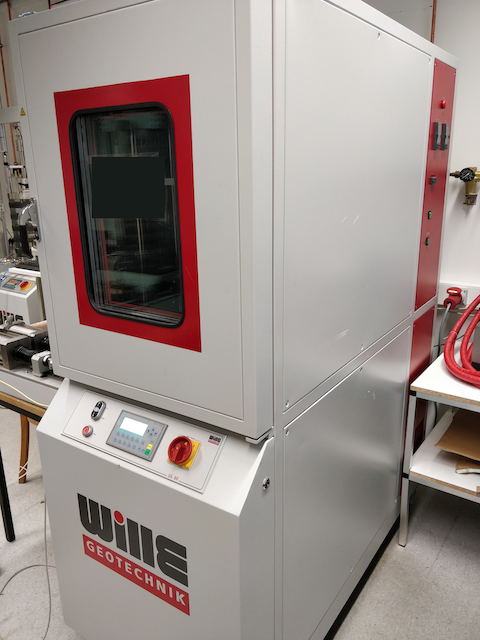
\includegraphics[width=4cm,height=5cm]{figures/Amir_Fracture_Toughness_Setup_b.png}
\subcaption{}
\label{fig:Amir_Fracture_Toughness_Setup_b}
\end{subfigure}
\caption{The required equipment for performing the three-point bending test (a) the loading cell and supports, (b) the climate chamber for controlling temperature and humidity}
\end{figure}

The claystone samples are prepared with the dimension of 140x30x30 $(mm)$ and the notch dimension of 2x10x30 $(mm)$v $(LxWxB)$  (Fig.\ref{fig:Amir_Fracture_Toughness_Sample}). The span length ($S_{flex}$) is 120 $mm$, which is 4 times the size of its width and thickness. The embedded layering is perpendicular to the loading direction. The image processing technique is used to track the reference points, which are predefined prior to the test procedure (Fig. \ref{fig:Amir_Fracture_Toughness_Image_a}). The distance between the points is measured using the optical microscopic image and is considered as an initial reading value (Fig. \ref{fig:Amir_Fracture_Toughness_Image_b}). The method is able to detect the minimum displacement of 2 micrometers, which is possible by taking 4k video with 30fps. The load vs. CMOD response of the Opalinus claystone as well as the numerical simulation outcomes are given in \ref{sec:mex01}. The effects of anisotropy and embedded layering orientation of Opalinus claystones on fracture toughness values are not fully studied. 

\begin{figure}[!ht]
\centering
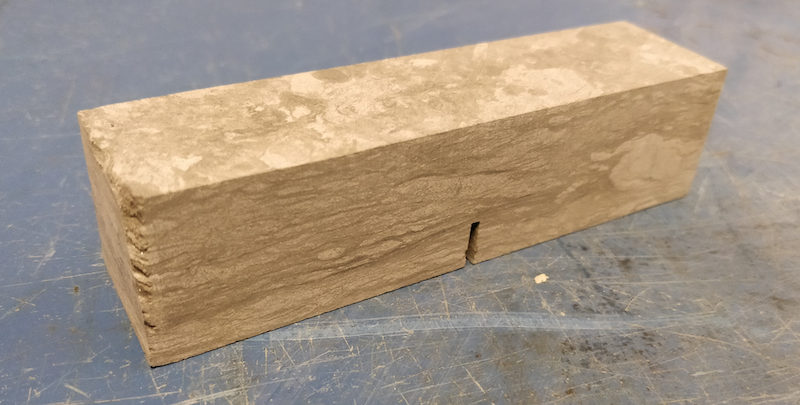
\includegraphics[width=8cm,height=4cm]{figures/Amir_Fracture_Toughness_Sample.png}
\caption{The prepared Opalinus claystone sample with the dimension of 140x30x30 $mm$}
\label{fig:Amir_Fracture_Toughness_Sample}
\end{figure} 

\begin{figure}[!ht]
\centering
\begin{subfigure}[c]{0.48\textwidth}
\centering
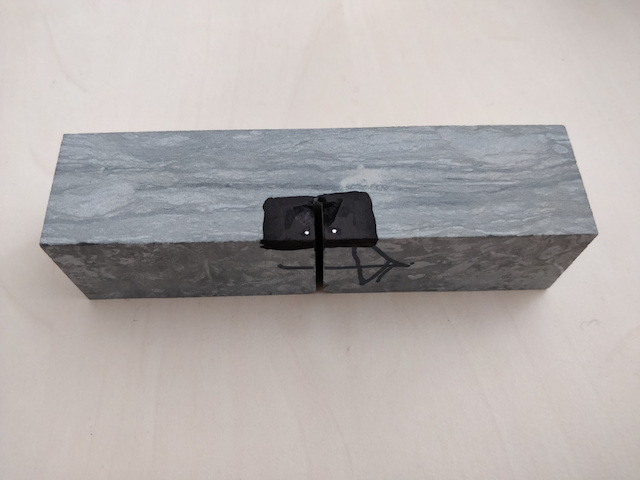
\includegraphics[width=6cm,height=5cm]{figures/Amir_Fracture_Toughness_Image_a.png}
\subcaption{}
\label{fig:Amir_Fracture_Toughness_Image_a}
\end{subfigure}
\hfill
\begin{subfigure}[c]{0.48\textwidth}
\centering
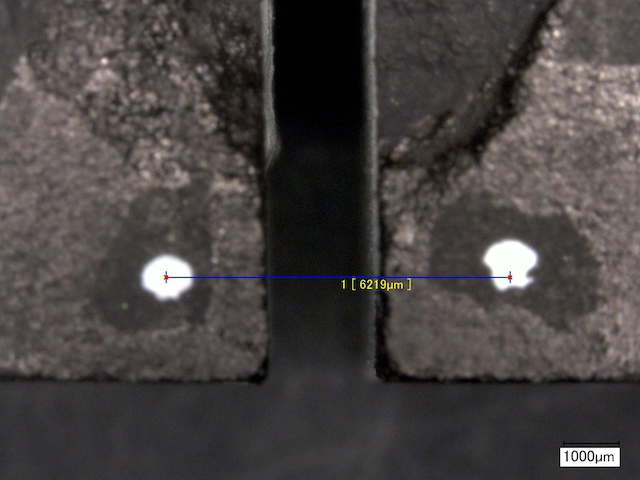
\includegraphics[width=6cm,height=5cm]{figures/Amir_Fracture_Toughness_Image_b.png}
\subcaption{}
\label{fig:Amir_Fracture_Toughness_Image_b}
\end{subfigure}
\caption{The application of image processing technique (a) the predefined reference points for measuring the CMOD, (b) the measured rough distance using optical microscope}
\end{figure}
%---------------------------------------------------------------------------------------------------
\subsection{Brazilian Disk Test on Barrier Rocks}
\label{sec:Brazilian_Disk_Exp}
\Authors{Amir Shoarian Sattari}
%\todo{Please insert authors}

The tensile strength of a brittle or quasi-brittle material, such as rock, is one of the most important material properties, which in comparison to the compression strength, is much weaker. The measurement of direct tensile strength of brittle materials is difficult and time consuming. Therefore, finding the splitting tensile strength ($\sigma_\text{sp}$) is a fast alternative for computing the direct tensile strength. The Brazilian disk test is conducted to determine the splitting tensile strength (Fig. \ref{fig:Amir_Splitting_Theory}). The splitting strength depends on loading rate, diameter and length of the specimen (\ref{eq:Splitting_Strength}). The works of \cite{Perras2014} and \cite{Li2013} provides a full review and a correlation between different rock strength properties.
\index{tensile strength}
\index{compression strength}
\index{Brazilian disk test}

\begin{figure}[!ht]
\centering
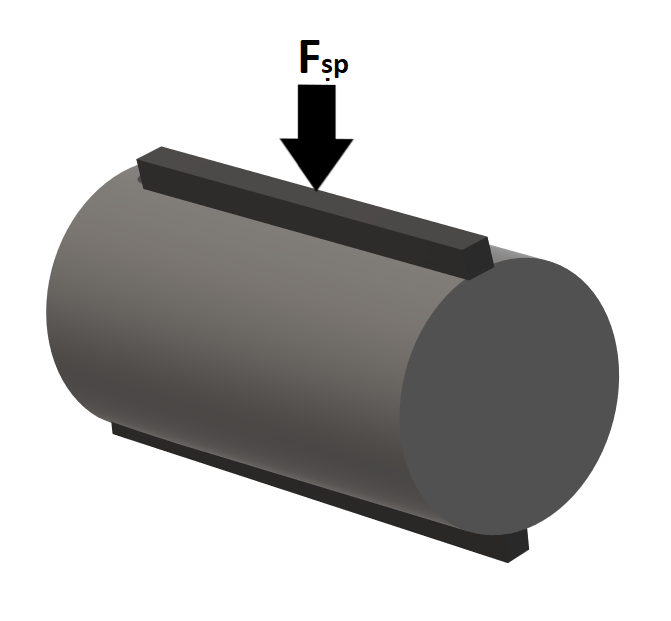
\includegraphics[width=6cm,height=5cm]{figures/Amir_Splitting_Theory.png}
\caption{The Brazilian disk test on a cylindrical sample with diameter and length of $D_\text{cyl}$ and $L_\text{cyl}$, respectively}
\label{fig:Amir_Splitting_Theory}
\end{figure} 

\begin{align}
\label{eq:Splitting_Strength}
\begin{split}
\sigma_\text{sp}=\frac{2f_\text{sp}}{\pi L_\text{cyl}D_\text{cyl}}
\end{split}
\end{align}

In the CAU Kiel laboratory, the splitting strength under THM processes is measured. To do so, a controlled temperature and humidity climate chamber (Fig. \ref{fig:Amir_Fracture_Toughness_Setup_b}) and a loading frame with a displacement transducer are required. Initially, the splitting test under room temperature condition with initial humidity of the sample is conducted. Afterwards, the temperature is raised to 50 and 80 $^{\circ}C$. The relative humidity can be controlled from 0 up to 100. Finally, the splitting strength, splitting Young’ modulus ($E_\text{sp}$) and load-displacement behavior are measured. The cylindrical claystone and saltstone samples are prepared in dimension of 100x200 $mm$ $(DxL)$ (Figure \ref{fig:Amir_Splitting_Sample}) and a strain rate of  0.1 \% is considered to insure a relatively fast loading rate. Fig. \ref{fig:Amir_Splitting_Setup} shows the placement of the sample under loading frame before performing the test.

\begin{figure}[!ht]
\centering
\begin{subfigure}[c]{0.3\textwidth}
\centering
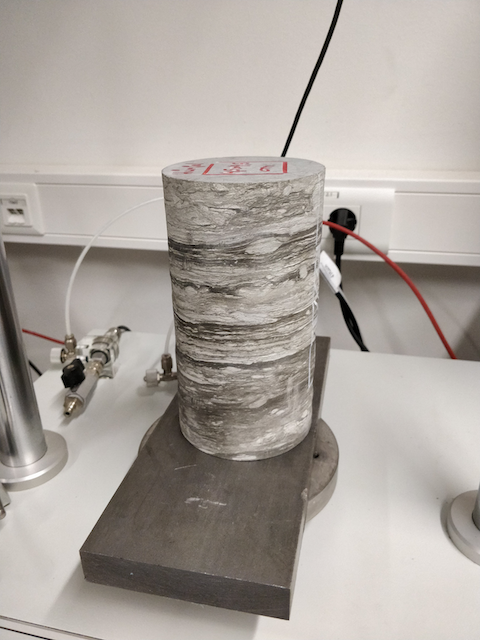
\includegraphics[width=4cm,height=5cm]{figures/Amir_Splitting_Sample.png}
\subcaption{}
\label{fig:Amir_Splitting_Sample}
\end{subfigure}
\hfill
\begin{subfigure}[c]{0.6\textwidth}
\centering
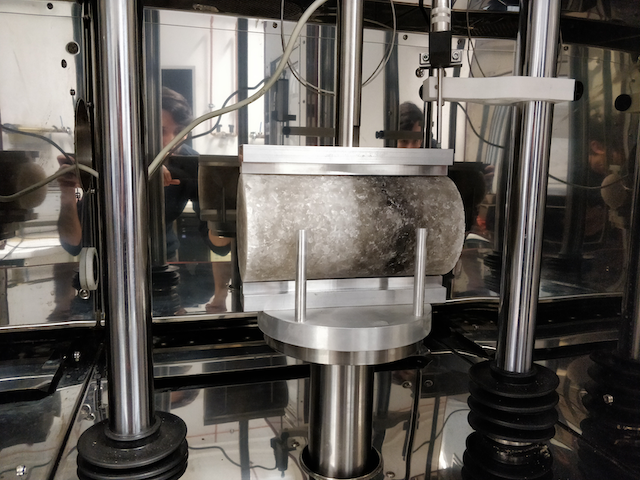
\includegraphics[width=6cm,height=5cm]{figures/Amir_Splitting_Setup.png}
\subcaption{}
\label{fig:Amir_Splitting_Setup}
\end{subfigure}
\caption{The sample preparation and test procedure (a) the claystone sample with a dimension of 100x200 $mm$, (b) the placement of saltstone inside of the climate chamber}
\end{figure}

Initially, the splitting strength of a saltstone samples under room temperature (20), 50 and 80 $^{\circ}C$ are measured. Due to a relatively homogeneous material property of the saltstone, the orientation of the sample will not affect the final outcomes. Figures \ref{fig:Amir_Splitting_Salt_20} and \ref{fig:Amir_Splitting_Salt_Result} depict the failure in 20 $^{\circ}C$ and load vs. displacement for different loading temperatures, respectively. The observed failure pattern for all of the setups is identical. The measured mean splitting strength using equation (\ref{eq:Splitting_Strength}) for 20, 50 and 80 $^{\circ}C$ are 1.65, 1.59 and 1.43 $MPa$, respectively. As a result, the temperature has a slight influence on the splitting strength of saltstone, especially when the temperature is raised up to 50 $^{\circ}C$.

\begin{figure}[!ht]
\centering
\begin{subfigure}[c]{0.35\textwidth}
\centering
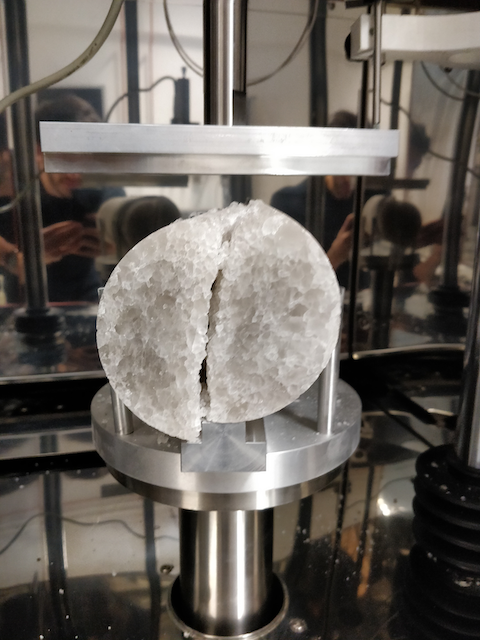
\includegraphics[width=4cm,height=5cm]{figures/Amir_Splitting_Salt_20.png}
\subcaption{}
\label{fig:Amir_Splitting_Salt_20}
\end{subfigure}
\hfill
\begin{subfigure}[c]{0.6\textwidth}
\centering
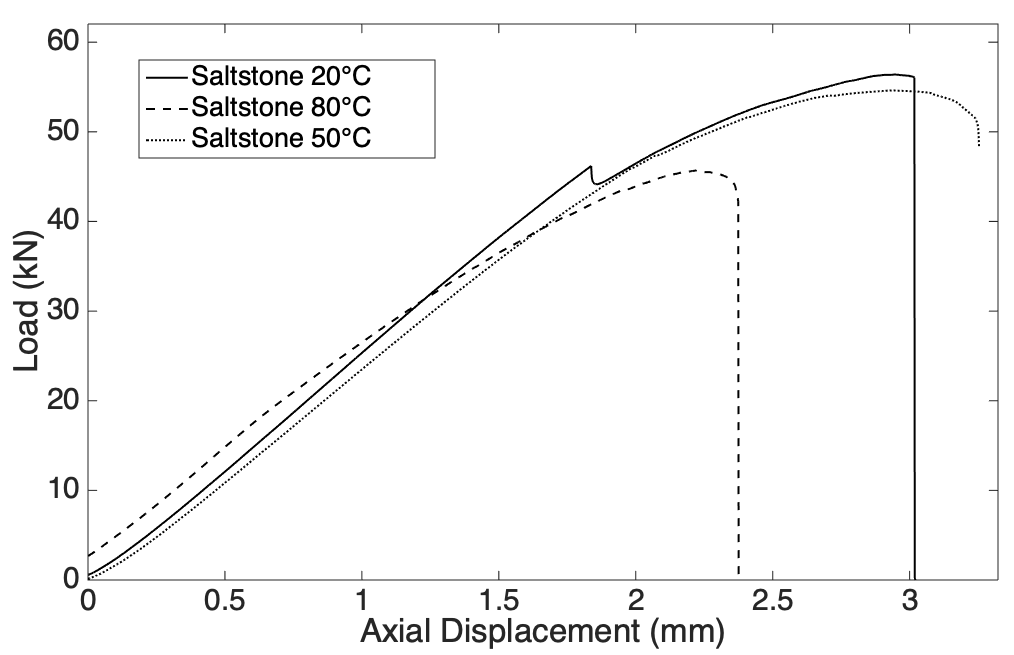
\includegraphics[width=6cm,height=5cm]{figures/Amir_Splitting_Salt_Result.png}
\subcaption{}
\label{fig:Amir_Splitting_Salt_Result}
\end{subfigure}
\caption{The splitting strength of a saltstone under different temperature conditions (a) the fracture path in saltstone in room temperature, (b) the load vs. displacement under different temperature conditions}
\end{figure}

The anisotropy of claystone and embedded layering orientation has a significant influence on material strength. To investigate the strength dependency on layering orientation, a series of tests, where the angle between the loading direction and layering orientation is 0 (parallel), 30, 45, and 90 (perpendicular) degree, is conducted. For 20 $^{\circ}C$, the failure pattern for 0, 45 and 90 degrees are provided in Figures \ref{fig:Amir_Splitting_Clay_0}, \ref{fig:Amir_Splitting_Clay_45} and \ref{fig:Amir_Splitting_Clay_90}. Fig. \ref{fig:Amir_Splitting_Clay_20_Result} depicts the load vs. displacement behavior of claystone with different layering degrees.
\index{anisotropy of claystone}

\begin{figure}[ht!]
\centering
\begin{subfigure}[c]{0.48\textwidth}
\centering
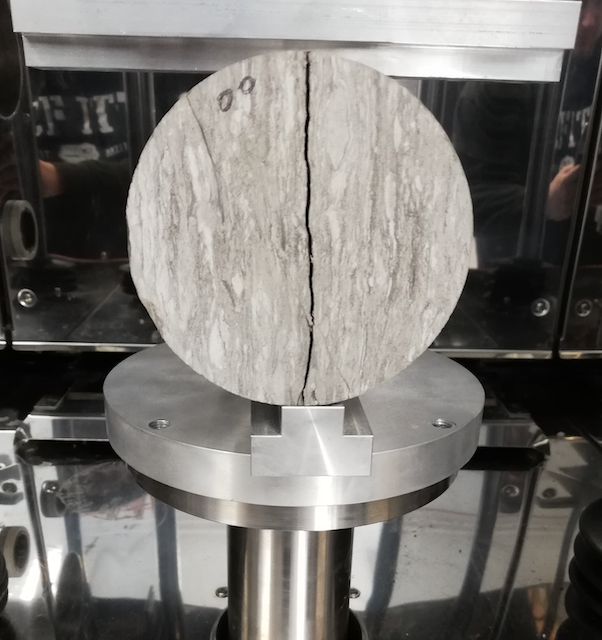
\includegraphics[width=5cm,height=5cm]{figures/Amir_Splitting_Clay_0.png}
\subcaption{}
\label{fig:Amir_Splitting_Clay_0}
\end{subfigure}
\hfill
\begin{subfigure}[c]{0.48\textwidth}
\centering
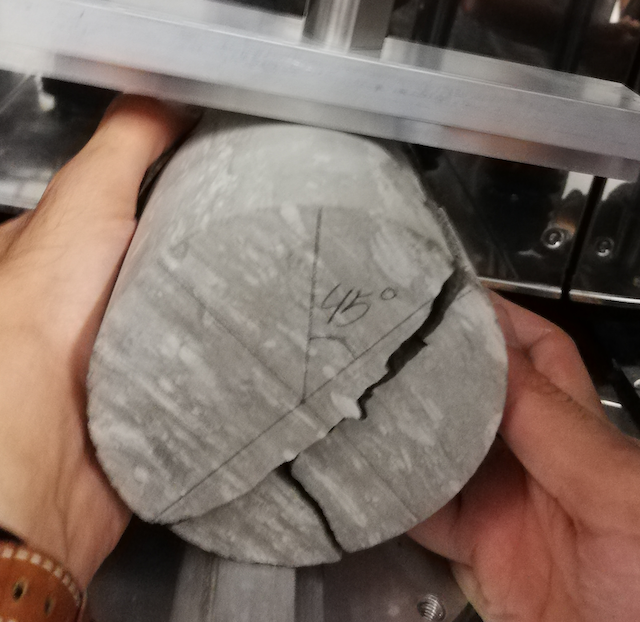
\includegraphics[width=5cm,height=5cm]{figures/Amir_Splitting_Clay_45.png}
\subcaption{}
\label{fig:Amir_Splitting_Clay_45}
\end{subfigure}
\hfill
\begin{subfigure}[c]{0.48\textwidth}
\centering
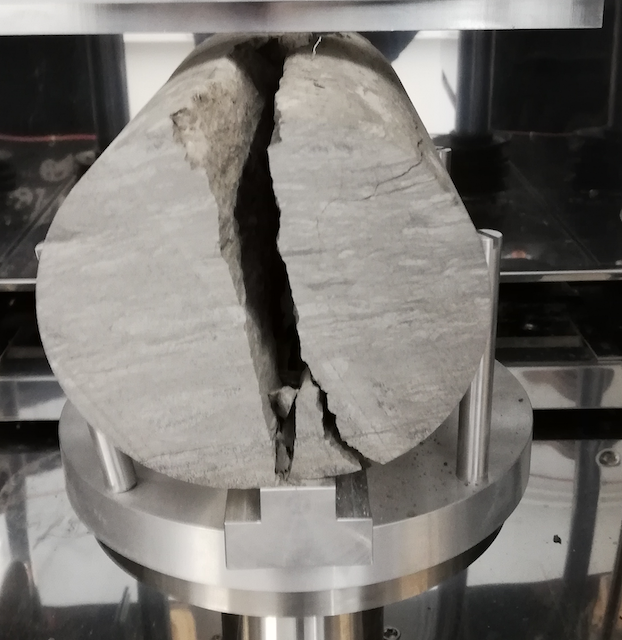
\includegraphics[width=5cm,height=5cm]{figures/Amir_Splitting_Clay_90.png}
\subcaption{}
\label{fig:Amir_Splitting_Clay_90}
\end{subfigure}
\caption{The fracture pattern under different layering orientation (a) 0 degrees, parallel, (b) 45 degrees, and (c) 90 degrees, perpendicular (20 $^{\circ}C$)}
\end{figure}

\begin{figure}[ht!]
\centering
\includegraphics[width=9cm,height=5cm]{figures/Amir_Splitting_Clay_20_Result.png}
\caption{The load vs. displacement under different layering orientation, 20 $^{\circ}C$}
\label{fig:Amir_Splitting_Clay_20_Result}
\end{figure} 

Table \ref{table:Amir_Splitting_Table1} presents the mean outcome of the experimental tests for different orientation angles and temperature. The results depicts that when the loading is perpendicular to the layering orientation, the splitting strength of the claystone is almost 5 times higher than when it is parallel to the layering orientation. The temperature effect on splitting strength is negligible. 

\begin{table}[!ht]
\centering
\begin{center}
\begin{tabular}{ | >{\centering\arraybackslash}X m{8em} | >{\centering\arraybackslash}X m{3em}| >{\centering\arraybackslash}X m{3em} | >{\centering\arraybackslash}X m{3em} | >{\centering\arraybackslash}X m{3em} | >{\centering\arraybackslash}X m{3em} | }
\hline
Test results & 0 $^{\circ}$ & 30 $^{\circ}$ & 45 $^{\circ}$ & 60 $^{\circ}$ & 90 $^{\circ}$ \\
\hline
$\sigma_\text{sp}$ ($MPa$) 20$^{\circ}C$ & 0.47 & 0.68 & 1.13 & 1.45 & 1.92  \\ 
\hline
$\sigma_\text{sp}$ ($MPa$) 80$^{\circ}C$ & 0.52 & 0.64 & 1.02 & 1.25 & 1.86   \\
\hline
\end{tabular}
\end{center}
\caption{The splitting tensile strength of the Opalinus claystone with different temperature and layering orientations}
\label{table:Amir_Splitting_Table1}
\end{table}

%---------------------------------------------------------------------------------------------------
%---------------------------------------------------------------------------------------------------
\subsection{True Triaxial Test on the Cubic Opalinus Claystone Samples}
\label{sec:True_Triaxial_Exp}
\Authors{Amir Shoarian Sattari (CAU)}
%\todo{Please insert authors}

The true triaxial apparatus, where the stresses are controlled along three axes, is used to investigate the three-dimensional strain-strength behavior of soil or rock geomaterial (Figure \ref{fig:Amir_TrueTriaxial_Apparatus}). The true triaxial device in the CAU Kiel laboratory is able to reach a mechanical loading of 600 $MPa$ as well as a thermal loading of up to 600 $^{\circ}C$. The cubic samples are prepared in the side dimension of 43 $mm$ and the edges are slightly curved in order to avoid the stress concentration and failure in the corners (Figure \ref{fig:Amir_TrueTriaxial_Sample}).

\begin{figure}[!ht]
\begin{subfigure}[c]{0.48\textwidth}
\includegraphics[width=1\textwidth]{figures/Amir_TrueTriaxial_Apparatus.png}
\subcaption{}
\label{fig:Amir_TrueTriaxial_Apparatus}
\end{subfigure}
\hfill
\begin{subfigure}[c]{0.48\textwidth}
\includegraphics[width=1\textwidth]{figures/Amir_TrueTriaxial_Sample.png}
\subcaption{}
\label{fig:Amir_TrueTriaxial_Sample}
\end{subfigure}
\caption{The (a) true triaxial apparatus in geomechanics laboratory of CAU Kiel, and (b) prepared cubic claystone sample with curved edges}
\end{figure}

The coupled thermo-mechanical loading conditions are considered in order to investigate the materials anisotropic stiffness along three axis, the elastic and plastic deformation under cyclic thermal and mechanical loadings, deviatoric stress field, and material failure. A thermal loading of up to $T_{iso}^{max}=150$ $^{\circ}C$ is considered, which is considered to be higher than the maximum temperature that the claystone samples are subjected to in nuclear waste disposal sites. The maximum isotropic mechanical loading is considered to be $\sigma_{iso}^{max}=100 MPa$, where $max$ and $c$ superscripts represent the maximum and constant values, respectively. The considered boundary conditions are:

\begin{list}{-}{\leftmargin=1em \itemindent=0em \itemsep=0.1em}
  \item Sample MT-01: Mechanical Condition,5 loading cycles, $\sigma_{iso}^{max}=100 MPa$.
  \item Sample MT-02: Coupled Thermo-Mechanical Condition, 4 loading cycles, $T_{iso}^{max}=150$ $^{\circ}C$ and $\sigma_{iso}^{c}=12 MPa$.
  \item Sample MT-03: Coupled Thermo-Mechanical Condition, 4 loading cycles, $T_{iso}^{max}=150$ $^{\circ}C$, and $\sigma_{iso}^{max}=100 MPa$.
  \item Sample MT-04: Coupled Thermo-Mechanical Condition, 4 loading cycles, $\sigma_{dev}^{max}=60 MPa$, $\sigma_{con}^{c}= 20 MPa$ and $T_{iso}^{c}=150$ $^{\circ}C$ .
\end{list}

With the installation of the ultrasonic sensors on the pistons, the apparatus is able to measure the ultrasonic $P$, $S90$ and $S0$ waves along the axis. The anisotropy factor, density ($\rho$), the dynamic Young’s modulus ($E_{Dyn}$), dynamic shear modulus ($G_{Dyn}$), and dynamic Poisson’s ratio ($\nu_{Dyn}$) values can all be calculated according to the analytical relation which already exist in the literature \cite{Motraetal2018} as given in equations (\ref{eq:YoungsModulus_Ultrasonic}) and (\ref{eq:PoissonsRatio_Ultrasonic}). In order to detect and analyse the ultrasonic signals in Opalinus Claystone, the minimum confining mechanical stresses of 12 $MPa$ is required. The test results of MT-01 (Figure \ref{fig:Amir_TrueTriaxial_MT_01_Result}) depicts the increment of the mean $E_{Dyn}$, $G_{Dyn}$ and $\nu_{Dyn}$ values under the isotopic confinement stresses up to 100 $MPa$, which is due to the layering orientation and structure of claystones and eventually improved contact qualities. It is also noted that the rate of the increment after each loading cycle (slope of the line) is decreased and due to the plastic deformations and improved contact qualities, the materials mechanical properties in initial loading condition of 12 $MPa$ are enhanced. 

\begin{figure}[ht!]
\centering
\begin{subfigure}[c]{0.48\textwidth}
\centering
\includegraphics[width=6cm,height=4cm]{figures/Amir_TrueTriaxial_MT_01_Result_E.png}
\subcaption{}
\end{subfigure}
\hfill
\begin{subfigure}[c]{0.48\textwidth}
\centering
\includegraphics[width=6cm,height=4cm]{figures/Amir_TrueTriaxial_MT_01_Result_G.png}
\subcaption{}
\end{subfigure}
\hfill
\begin{subfigure}[c]{0.48\textwidth}
\centering
\includegraphics[width=6cm,height=4cm]{figures/Amir_TrueTriaxial_MT_01_Result_Nu.png}
\subcaption{}
\end{subfigure}
\caption{The true triaxial results for the MT-01 sample under 5 loading cycles (a) $E_{Dyn}$ vs. Confinement Stress, (b) $G_{Dyn}$ vs. Confinement Stress, and (c) $\nu_{Dyn}$ vs. Confinement Stress}
\label{fig:Amir_TrueTriaxial_MT_01_Result}
\end{figure}

Figure \ref{fig:Amir_TrueTriaxial_MT_02_Result} shows the deformation vs. time result of MT-02 in the 1st cycle. The thermal plastic deformation after 5 cycles of loading and unloading was negligible and can be neglected. The MT-02 sample is situated in a way that the loading frame in direction of Z is parallel to the layering orientations of claystone. The volumetric thermal expansion coefficient ($\alpha_V$) is calculated based on the measured volumetric strain ($\epsilon_V=\frac{\Delta V}{V}$) and temperature change ($\Delta T$). The effect of temperature on $\alpha_V$ is shown at Figure \ref{fig:Amir_TrueTriaxial_MT_02_Result_1a}. The rate of $\alpha_V$ is decreased after 80 $^{\circ}C$. The anisotropy in linear thermal expansion coefficient along Z, Y and X axis is shown in Figure \ref{fig:Amir_TrueTriaxial_MT_02_Result_1b}. The anisotropy in the measured linear expansion coefficient ($\alpha_{Li}$) is substantially decreased after 80 $^{\circ}C$.

\begin{align}
\label{eq:ThermalExpansion}
\begin{split}
\alpha_V=\frac{\epsilon_V}{\Delta T}=\frac{\Delta V}{V\Delta T}
\end{split}
\end{align}

\begin{figure}[!ht]
\centering
\includegraphics[width=7cm,height=4cm]{figures/Amir_TrueTriaxial_MT_02_Result.png}
\caption{The deformation vs time for sample MT-02}
\label{fig:Amir_TrueTriaxial_MT_02_Result}
\end{figure} 

\begin{figure}[!ht]
\centering
\begin{subfigure}[c]{0.48\textwidth}
\centering
\includegraphics[width=6cm,height=4cm]{figures/Amir_TrueTriaxial_MT_02_Result_1a.png}
\subcaption{}
\label{fig:Amir_TrueTriaxial_MT_02_Result_1a}
\end{subfigure}
\hfill
\begin{subfigure}[c]{0.48\textwidth}
\centering
\includegraphics[width=6cm,height=4cm]{figures/Amir_TrueTriaxial_MT_02_Result_1b.png}
\subcaption{}
\label{fig:Amir_TrueTriaxial_MT_02_Result_1b}
\end{subfigure}
\caption{The effect of temperature on (a) $\alpha_V$, and (b) the anisotropy in the linear thermal expansion coefficient ($\alpha_{Li}$)}
\end{figure}

The test results of MT-03 investigates the anisotropy of Opalinus claystone samples. Figure \ref{fig:Amir_TrueTriaxial_MT_03_Result} illustrates the $1^{st}$ cycle loading results of $E_{Dyn}$ and $\nu_{Dyn}$ values in X, Y and Z directions under the isotopic confinement stresses up to 100 $MPa$. The $G_{Dyn}$ has a similar behavior to the $E_{Dyn}$ values. The results indicate a weaker stiffness in Z direction, which is parallel to the layering orientation. The thermal loading upto 150 $^{\circ}C$ results in weaker $E_{Dyn}$ values during the heating process, which is the reason for the fluctuation of the results at the confinement stress of 100 $MPa$. The test results of MT-04 is similar to the MT-02 and the same material response is observed. 

\begin{figure}[ht!]
\centering
\begin{subfigure}[c]{0.48\textwidth}
\centering
\includegraphics[width=6cm,height=4cm]{figures/Amir_TrueTriaxial_MT_03_Result_E.png}
\subcaption{}
\end{subfigure}
\hfill
\begin{subfigure}[c]{0.48\textwidth}
\centering
\includegraphics[width=6cm,height=4cm]{figures/Amir_TrueTriaxial_MT_03_Result_Nu.png}
\subcaption{}
\end{subfigure}
\caption{The true triaxial results for the MT-03 sample in the $1^{st}$ cycle (a) $E_{Dyn}$ vs. Confinement Stress, and (b) $\nu_{Dyn}$ vs. Confinement Stress}
\label{fig:Amir_TrueTriaxial_MT_03_Result}
\end{figure}
\clearpage
%---------------------------------------------------------------------------------------------------
\subsection{Triaxial compression strength tests for salt - methodology and equipment}
\index{TC triaxial compression test}

Triaxial compression tests (TC) are executed on cylindrical core samples with dimensions of e.g. 200*100 mm (generally a 2:1 ratio of height to diameter) in one of two available servo-hydraulic testing machines of the IfG labs (RBA 2500, Schenk/Trebel, Germany and D2000 GGL Testsystems – using the MTS-TestStar software; see Fig. \ref{fig:ifglabph2} generating the necessary stress $\sigma_1$ in axial direction and $\sigma_3$ in lateral direction.

The cylindrical samples are sealed with rubber tubes and oil is used as confining medium. Outside the vessel three LVDT transducers are mounted between the piston and the load frame near the sample for the measurement of the axial strain. The axial load is determined from an external load cell. Tests can also be carried out at in-situ relevant temperatures (e.g. 55$^\circ$C). During all tests the following parameters are measured automatically: the axial deformation $\Delta h$, axial load $F$ and the confining pressure $p = \sigma_3$. The conversion of the measured values to effective stress and strain is given as:

\begin{equation}
\sigma_\text{eff} = \left(\frac{F}{A_0}-\sigma_3 \right) (1-\epsilon_1)
\end{equation}
\begin{equation}
\epsilon_1 = \frac{h_0-h}{h_0}
\end{equation}
with
\begin{tabbing}
symbo \= description \kill
$h_0$, $h$ : \> length of the sample before and during deformation \\
$A_0$ : \> cross sectional area of the undeformed sample \\
$F$ : \> axial load  \\
$\sigma_3$ : \> confining pressure 
\end{tabbing}

The term $1-\epsilon_1$ results from the consideration of the sample bulge during the deformation, e.g. the changes of the cross sectional area as well in compression as in extension are regarded.

In addition, as a standard technique of the IfG during the triaxial strength experiments the sample volume changes $\Delta V$ are determined by a volume balance of the mantle oil volume changes as measured via the pressure intensifier and the axial piston displacement in the cell:

\begin{equation}
\Delta V = \Delta h A_{pp} -\Delta S_{pi} A_{pi}
\end{equation}
with
\begin{tabbing}
symbo \= description \kill
$\Delta h$ : \> displacement of the piston of the triaxial cell \\
$A_{pp}$ : \> cross section of the piston of the triaxial cell \\
$\Delta S_{pi}$ : \> displacement of the cylinder within the pressure intensifier \\
$A_{pi}$ : \> cross section of the piston within the pressure intensifier \\
\end{tabbing}

During all tests the following parameters were measured automatically: The axial deformation $\Delta h$, axial load $F$ and the confining pressure $p = \sigma_3$. 

\begin{figure}[!ht]
\centering
\includegraphics[width=0.5\textwidth]{./figures/ifg-lab-photo3.png}
\caption{The two available servo-controlled hydraulic testing machines (right: system RBA 2500 of SCHENK/TREBEL and left: D2000 of GGL TestSystems)}.
\label{fig:ifglabph2}
\end{figure}

The triaxial test procedure is divided into two steps:

\begin{list}{-}{\leftmargin=1em \itemindent=0em \itemsep=0.2em}
\item 1st step: Reconsolidation – isotropic phase (applied for all samples): Because it is assumed that core material is generally dilated due the applied procedures during core recovery (stress relaxation) and subsequent weathering, the samples are firstly re-compacted. In a hydrostatic load cycle ($\sigma_1 = \sigma_3$) the samples are pressurized up to 60 MPa (at 0.01 MPa/s) and then, after 30 min. unloaded to the respective pressure state of the strength test.
\item 2nd step: Triaxial test cycle – deviatoric phase:  At constant confining pressure the sample is axially loaded using a constant deformation rate, until the sample fails and reaches the post failure state. Common standard triaxial compression tests (TC) with defined deformation rate at constant confining pressures are between 1 and 25 MPa. A determination of the deformation dependent strength and dilatancy behavior is realized, too.
\end{list}
\index{dilatancy}

The standard triaxial strength test (TC) for salt rocks is performed with a constant deformation rate 
(5$\cdot$10$^{-6}$ s$^{-1}$) at constant confining pressure. After the failure occurs the axial load decreases with further deformation due to the decrease of the load-bearing capacity becoming nearly constant if the post-failure stage is reached. Finally the sample is unloaded.

Simultaneously with the deformation the volumetric strain is measured which allows to determine the 
stress-dependent onset of micro-cracking (given by the minimum) and to quantify the deformation induced damage.



%---------------------------------------------------------------------------------------------------
\clearpage
%===================================================================================================
\section{Shrinkage and Swelling Laboratory Tests (WP1)}
\label{sec:lab-wp1}
\subsection{The Swelling Characteristic of the Opalinus Claystone}
\Authors{IfG}
\todo[inline]{[IfG](): The description of the experiment procedure}

%---------------------------------------------------------------------------------------------------
%\subsection{Oedometer Test (BGR)}
%---------------------------------------------------------------------------------------------------

\subsection{The Wetting and Drying Paths of the Opalinus Claystone}
\label{sec:Shrinkage_Swelling_Exp}
\Authors{CAU Kiel}
%\todo{Please insert authors}

The shrinkage and swelling of claystone results in micro fracking and higher permeability values, which in nuclear waste disposal sites can lead to contamination of groundwater. Micro fracking also decreases the strength of the material subjected to THM  loading processes. Typically, the swelling pressure and heave of claystone is determined using Oedometer tests \cite{Peronetal2009}, where a constrained or unconstrained sample is subjected to the swelling process (Figure \ref{fig:Amir_Shrinkage_Swelling_Setup}). During the test procedure, the swelling pressure, as well as the heave magnitude, are recorded. It is observed that the swelling pressure in sandy facies of claystone is lower than shaly facies. In contrast to the swelling tests, shrinkage tests are less common and are complicated to perform on rock materials. \cite{Minardietal2016} performed a shrinkage test on claystone with shaly and sandy facies using a desiccator and various salt solutions (Figure  \ref{fig:Amir_Shrinkage_Minardi}). During the test procedure the axial strain values obtained from the strain gauges, as well as sample weight, are measured.

\begin{figure}[!ht]
\begin{subfigure}[c]{0.48\textwidth}
\includegraphics[width=1\textwidth]{figures/Amir_Shrinkage_Swelling_Setup.png}
\subcaption{}
\label{fig:Amir_Shrinkage_Swelling_Setup}
\end{subfigure}
\hfill
\begin{subfigure}[c]{0.48\textwidth}
\includegraphics[width=1\textwidth]{figures/Amir_Shrinkage_Minardi.png}
\subcaption{}
\label{fig:Amir_Shrinkage_Minardi}
\end{subfigure}
\caption{The swelling and shrinkage tests on Opalinus claystone (a) the Oedometer test setup for constrained swelling pressure in Opalinus clay samples \cite{Peronetal2009}, and (b) measuring the drying and wetting paths using desiccator \cite{Minardietal2016}}
\end{figure}

Two prepared thin cylindrical sections of sandy Opalinus claystone (Mont-Terri) with a dimension of 100x10 $mm (DxH)$ are used to determine the anisotropy in shrinkage and swelling behavior of claystone. Due to the mineral structure of claystone and its layering orientation, the anisotropy factor has a significant influence on the direction of shrinkage and swelling as well as the micro fracking formation. The initial sample is used to determine the axial strains in parallel and perpendicular directions to the layering orientations. The strain gauge strips (HBM, $LY 10 (mm)$/120 $\Omega$) are glued and attached to the surface of the sample. The second sample is used to measure the weight change in the sample under different salt solutions. The saturated salt solutions are located inside the desiccator and will result in osmotic suction and eventually in the wetting and drying of the samples. The total suction($\psi_{total}$) value can be measured using the Kelvin’s relation, which is derived from ideal gas law:

\begin{equation}
\label{eq:Total_Suction}
\psi_{total} = \frac{RT}{V_{mol}} \ln(\frac{P_{vap}^{cur}}{P_{vap}^{cur=0}})
\end{equation}

where, $(\frac{P_{vap}^{cur}}{P_{vap}^{cur=0}})$ is the relative humidity, $P_{vap}^{cur=0}$ is the vapor pressure when the surface curvature is equal to zero (flat surface), $R$ is the universal gas constant, $T$ is the temperature and $V_{mol}$ is the molecular volume of water. The equilibrium inside the desiccator is reached when the strain gauges value or water content of the samples are constant in two consecutive readings. The results obtained from the drying and wetting paths of the Opalinus claystone are given in \ref{sec:mex06}, where a numerical simulation and comparison to the experimental data are provided. The test procedure is time consuming and after measuring the data for more than 120 days, the applied suction and water content percentages are calculated and plotted. 

%---------------------------------------------------------------------------------------------------
\subsection{In-situ Condition Desiccation Process (Stuttgart or BGR)}
\todo[inline]{[UoS/BGR](): More description please}
Topology, respectively morphology investigations of fractures induced in clay stone throughout drying processes require a number of experimental sequences ranging from the drying process itself to characterization of the induced fractures by X-Ray Computed Tomography. The required samples are prepared and characterized by the University of Kiel with a dimension of radius $r = 5 \, \text{mm}$ and height $h = 50 \, \text{mm}$ to guarantee the realization of scans in Regions of Interests (RoIs) down to a characteristic edge length of $6 \, \text{mm}$ resulting in a resolution of 2 micrometers per voxel.

Two different experimental set-ups are planned; nevertheless the first proposed experimental implementation is preferred over the second.

\subsection{Drying Wet Samples - From Wet to Dry}
\todo[inline]{[UoS](): More description please}
Saturated samples are prepared by the University of Kiel and submerged in a shrink tube in order to minimize the change of the desired state. Once the experiments are performed on the sample the shrink tube is removed and the probe is installed in an uni-axial testing device. The sample is installed in a heat chamber and loaded by an axial force of $f_{ax} = 500 \, \text{N}$/, resulting in an axial stresses of $ \sigma_{ax} = 0.25 \text{MPa}$ (potentially up to $f_{ax} = 5 \, \text{kN}$/$ \sigma_{ax} = 2.5 \text{MPa}$) while axial deformations are measured under controlled temperature conditions. By measuring the sample's weight at characteristic states (twice - beginning and end) the volumetric deformations can be determined and related to the change of saturation. The sample characterization is then completed by XRCT scans to determine the features of the induced fractures. Finally the stiffness degradation is determined by ultrasound experiments measuŕing the P-wave run times at 2, respectively 6 MHz.

\subsection{Wetting dry Samples - From Dry to Wet}
\todo[inline]{[UoS](): More description please}

Since it is extremely time consuming to increase the saturation of the sample this second setting is only an alternative to the introduced set-up in case the first experiment fails. The set-up is comparable to the proposed experiment but performed in a heat-humidity chamber at rel. humidity between 10 - 90 \% and temperatures between $5-90^\circ C$. The applied axial Force would reduce to $f_{ax} = 50 \, \text{N}$.
\clearpage
%---------------------------------------------------------------------------------------------------
\section{Pressure Driven Percolation Laboratory Tests (WP2)}
\label{sec:lab-wp2}
%===================================================================================================
%---------------------------------------------------------------------------------------------------
\subsection{Pressure Driven Percolation}
\Authors{IfG}
%\todo{Please insert authors}

The determination of the permeability, which quantifies the flow behavior of fluids in the pore space of a rock, is based on the Darcy equation:
\index{Darcy equation}

\begin{equation}
q = \frac{kA}{L\eta}\Delta p
\end{equation}

with:
\begin{tabbing}
sym \= description \kill
$q$ : \> flow rate (m$^3$/s) \\
$k$ : \> permeability (m$^2$) \\
$A$ : \> cross sectional area (m$^2$) \\
$L$ : \> length of sample (m) \\
$\eta$ : \> dynamic viscosity (Pa$\cdot$ s) \\
$\Delta p$ : \> pressure difference (Pa)
\end{tabbing}

Thereafter, the flow rate of a fluid through a sample at a given pressure differential is measured by the viscosity of the flowing medium, the geometric factor of the sample, and the permeability (with the dimension of an area). The permeability is given as SI-unit in (m$^2$ or, traditionally, in D (Darcy) (1 D corresponds to about 10$^{-12}$ m$^2$).

The equation above is only valid for incompressible fluids, because only then is the flow rate $q$ constant over the flow path. With sufficient accuracy, this applies to low compressible fluids.
When a gas flows through the pore space of a solid, however, an expansion of the gas takes place along the flow path, so that the flow rate is not constant here. In this case, instead of the flow rate $q$ the mean flow rate $q_m$ is set, for which, for small pressures with sufficient accuracy according to the law of Boyle-Mariotte:
\index{Boyle-Mariotte law}

\begin{equation}
q_m p_m = q_0 p_0
\end{equation}

with:
\begin{tabbing}
sym \= description \kill
$q_m$ : \> mean flow rate \\
$p_m$ : \> mean pressure \\
$q_0$ : \> measured flow rate at $p_0$ \\
$p_0$ : \> pressure at flow rate measurement 
\end{tabbing}

If, for the mean pressure $p_m$, the arithmetic mean of the pressures $p_1$ on the high pressure side and $p_2$ on the low pressure side of the porous solid is used, taking into account that $\Delta p = p_1 - p_2$, the modified Darcy equation for gas flows is as follows:

\begin{equation}
k = \frac{2p_0q_0\eta L}{A(p_1^2-p_2^2)}
\end{equation}

In summary, the determination of the permeability with caustic or gas with knowledge of the viscosity requires in each case an exact measurement of the flow rate after setting (quasi) stationary flow conditions and the pressure gradient.

To carry out permeability tests, the IfG Leipzig uses a servo-hydraulic testing machine with a pressure cell up to pc-max = 1000 bar, which is otherwise used for strength tests with $F_{max}$ = 2500 kN (manufacturer: Schenk / Trebel) (Fig. \ref{fig:ifglabph4}). The tests routinely set hydrostatic pressure conditions ($\sigma_1 = \sigma_2 = \sigma_3$), but it is also possible to implement deviatoric stresses or defined deformations. The axial load or deformation and the jacket pressure are each controlled 
independently via a servo-hydraulic system. 

The desired jacket pressure is generated by a pressure intensifier. From the axial deformation and the measured change in volume of the lateral pressure chamber (piston displacement of the pressure booster), the volume change of the test specimen, referred to here as dilatancy, can be determined at constant jacket pressure.

In hydrostatic loads sintered metal plates are used, which allow over the entire cross-sectional area of the sample a fluid pressurization. The pressure measurement of the measuring fluid is carried out by pressure transducers from Hottinger (accuracy class 0.2), whereby depending on the measuring range a 20 bar or 200 bar encoder is used.

\begin{figure}[!ht]
\centering
\includegraphics[width=1\textwidth]{./figures/ifg-lab-photo4.png}
\caption{Triaxial IfG pressure cell for flow tests with brine or gas.}
\label{fig:ifglabph4}
\end{figure}

The measuring principle for permeability determination under stationary conditions is based on the measurement of the flow rate $q$, here under atmospheric conditions ($p_0$), in the axial sample direction at a predetermined pressure gradient $\Delta p = p_1 - p_2$ ($p_1$ = inlet pressure, $p_2$ = outlet pressure).

The measuring arrangement used in the triaxial cell has the following advantages over the frequently used Hassler cells, in which a cylindrical sample is firmly clamped between punches and is only subjected to radial pressure.

\begin{list}{-}{\leftmargin=1em \itemindent=0em \itemsep=0em}
\item Determination of sample deformation during hydrostatic and deviatoric pressurization
\item Use of variable sample geometries (stamp sets between 60 and 110 mm diameter are available, height up to 2 x diameter)
\item The height of the gas injection pressure is limited only by the available gas cylinder pressure (routinely max: 200 bar).
\item For higher gas pressures (up to 1000 bar), a Maximator pneumatic pressure booster is used, but this is only used for special measurements.
\end{list}

For the determination of gas permeability two methods are available:
\begin{list}{-}{\leftmargin=1em \itemindent=0em \itemsep=0.1em}
\item 1st: Injection of nitrogen at a defined injection rate within a range of min. 0.1 ml / min to max. 500 ml / min under 
measurement of the injection pressure when stationary conditions are reached with leakage of the fluid against the atmosphere.
\item 2nd: Injecting nitrogen under a defined pre-pressure and measuring the flow rate at the exit side of the sample against the atmosphere.
\end{list}

\begin{figure}[!ht]
\centering
\includegraphics[width=1\textwidth]{./figures/ifg-perme-flowrate.png}
\caption{Variation diagram of permeability vs. flow rate for a sample with l = 220 mm and d = 110 mm at different injection pressures.}
\label{fig:ifgpermeflow}
\end{figure}

The lower limit of the measuring range depends essentially on the pre-pressure or the minimum measurable flow rate, as shown schematically in Fig. \ref{fig:ifgpermeflow}.
%
For gas permeability measurements, EL-FLOW mass flow controllers or flow meters from Bronkhorst are used with the following specifications:

\begin{list}{-}{\leftmargin=1em \itemindent=0em \itemsep=0em}
\item Mass flow controller Type: F-230M: Measuring range: (0) ... 10 ... 500 ml / min N2
\item Form: 200 bar / outlet pressure: 194 bar / temperature: 20$^\circ$C
\item Measuring accuracy: ± 1\% of final value, typ. better 0.5\%
\item Mass flow controller Type: F-230M: Measuring range: (0) ... 0.4 ... 20 ml / min
\end{list}

%---------------------------------------------------------------------------------------------------

\subsection{Fluid Driven Percolation Tests on Cubic Opalinus Claystone samples from Mont-Terri}
\label{sec:Percolation_Claystone_Exp}
\Authors{CAU Kiel}
%\todo{Please insert authors}

The investigation of a fluid transport in claystone due to its anisotropic behavior and its role as a rock barrier in nuclear waste repositories has a great importance. Performing hydraulic fracking under pressurized fluid or storing pressurized fluids leads to the fracking of rock barrier and fluid transport through the hydraulic apertures and cavities. This can lead to pressure and volume drop in the reservoir, decrease the output and efficiency of the designed system and the contamination of ground water. In the geomechanics laboratory of CAU Kiel, the true triaxial apparatus with the maximum mechanical pressure of 600 $MPa$ and thermal loading up to 600 $^{\circ}C$ is used to conduct the fluid driven percolation in claystone samples from Mont-Terri (Figure \ref{fig:Amir_TrueTriaxial_Apparatus}). The syringe pump, with the maximum pressure of 517 $bar$, is used to pressurize the oil fluid. The cubic samples with the side dimension of 43 $mm$ and center hole length and diameter of 20 and 8 $mm$ are prepared (Figure \ref{fig:Amir_Percolation_Adapter}), respectively, and attached to the pump pipes, where the sealing is done with O-rings and epoxy glue (Figure \ref{fig:Amir_Percolation_Setup}). 

\begin{figure}[!ht]
\begin{subfigure}[c]{0.48\textwidth}
\includegraphics[width=6cm,height=4cm]{figures/Amir_Percolation_Adapter.png}
\subcaption{}
\label{fig:Amir_Percolation_Adapter}
\end{subfigure}
\hfill
\begin{subfigure}[c]{0.48\textwidth}
\includegraphics[width=6cm,height=4cm]{figures/Amir_Percolation_Setup.png}
\subcaption{}
\label{fig:Amir_Percolation_Setup}
\end{subfigure}
\caption{The fluid driven percolation test preparation (a) the prepared cubic claystone sample and the adapter¸ and (b) the sample placement inside the true triaxial apparatus}
\end{figure}

Two different stress configurations, as well as fluid injection directions parallel or perpendicular to the layering orientation, are considered to investigate the fracking pattern as well as flow pathways. The fracking tests are carried out under a constant fluid pressure and the peak fluid pressure, where the flow rate increases and any sudden drops in fluid pressure is recorded. In the initial test, a sample with a fluid injection direction perpendicular to the layering orientation of the Opalinus sample is considered (Figure \ref{fig:Amir_Percolation_Orientation1}). The initial stress configuration is 12, 14 and 16 $MPa$ in three different loading directions (Figure \ref{fig:Amir_Percolation_Stress_1}). In order to prevent damaging the sample prior to the hydraulic fracking test, the isotropic stresses of 8 $MPa$ is applied from all pistons and is then gradually increased to the planned stress configuration. The oil pressure is increased gradually up until the point where the borehole pressure drops and an increase in the flow rate can be seen. The test is then aborted immediately in order to avoid causing any damage to the true triaxial apparatus. In the second test setup, a sample with a fluid injection direction parallel to the layering orientation of the Opalinus sample is considered (Figure \ref{fig:Amir_Percolation_Orientation2}). The initial stress configuration is 16, 10 and 8 $MPa$ in three different loading directions (Figure \ref{fig:Amir_Percolation_Stress_2}).

\begin{figure}[!ht]
\begin{subfigure}[c]{0.48\textwidth}
\includegraphics[width=4cm,height=4cm]{figures/Amir_Percolation_Orientation1.png}
\subcaption{}
\label{fig:Amir_Percolation_Orientation1}
\end{subfigure}
\hfill
\begin{subfigure}[c]{0.48\textwidth}
\includegraphics[width=5cm,height=4cm]{figures/Amir_Percolation_Stress_1.png}
\subcaption{}
\label{fig:Amir_Percolation_Stress_1}
\end{subfigure}
\caption{The boundary conditions for the $1^{st}$ stress configuration (a) the orientation of the embedded layers, and (b) the initial stress configuration}
\end{figure}

\begin{figure}[!ht]
\begin{subfigure}[c]{0.48\textwidth}
\includegraphics[width=4cm,height=4cm]{figures/Amir_Percolation_Orientation2.png}
\subcaption{}
\label{fig:Amir_Percolation_Orientation2}
\end{subfigure}
\hfill
\begin{subfigure}[c]{0.48\textwidth}
\includegraphics[width=5cm,height=4cm]{figures/Amir_Percolation_Stress_2.png}
\subcaption{}
\label{fig:Amir_Percolation_Stress_2}
\end{subfigure}
\caption{The boundary conditions for the $2^{nd}$ stress configuration  (a) the orientation of the embedded layers, and (b) the initial stress configuration}
\end{figure}

The results of the percolation tests on the Opalinus claystone samples are given in \ref{sec:mex02}, where a numerical simulation and comparison to the experimental data are provided and the effect of stress distribution, anisotropy and layering orientation on frack paths and fracking pressure are discussed. 

extra comment: change the title of 2.4.1 to be more specific (to show the difference between 2.4.1 and 2.4.2). I suggest: Pressure Driven Percolation Tests on Cylindrical Samples
\clearpage
%---------------------------------------------------------------------------------------------------
\section{Stress Redistribution Laboratory Tests (WP3)}
\label{sec:lab-wp3}
\subsection{Direct Shear Test}
%---------------------------------------------------------------------------------------------------
\Authors{Thomas Fr\"uhwirt, Daniel P\"otschke}

To conduct direct shear tests special equipment is necessary. The direct shear testing device at the rock mechanical laboratory of the TU Freiberg (see Fig. \ref{fig:ExpCNLShearMachine}) is specially developed to ensure the wanted functionality.

\begin{figure}[!ht]
\begin{center}
\includegraphics[width=0.6\textwidth]{./figures/ExpShearMachine.jpg}
\end{center}
\caption{The shear testing device at the rock mechanical laboratory of the TU Freiberg. (From: \cite{Konietzky2012})}
\label{fig:ExpCNLShearMachine}
\end{figure}

Some key features can be found in Table \ref{table:ExpCNLDeviceTechnicalData}. Additionally it is possible to superimpose dynamic forces. In the tests for the GeomInt project this functionality was not used.

\begin{table}[!ht]
\begin{center}
\begin{tabular}{l r r}
Feature & Value & Unit\\
\hline
Max. normal force & 1000 & kN\\
Max. shear displacement & 50 &mm\\
Min. shear velocity & 1e-7 & mm/s\\
Max. shear velocity & 70 & mm/s\\
Max. sample size (rectangular) & 200$\times$400 & mm\\
Max. fluid pressure & 10 & MPa\\
\end{tabular}
\caption{Technical data of the shear testing device. (From: \cite{Konietzky2012})}
\label{table:ExpCNLDeviceTechnicalData}
\end{center}
\end{table}

The sample preparation includes the cutting of the rock block in the cuboid shape. This sample is split into two parts and the rock joints are arranged in a matching position. It is arranged in the shear box, Fig. \ref{fig:ExpCNLSampleInShearBox}.

\begin{figure}[!ht]
\begin{center}
\includegraphics[width=0.6\textwidth]{./figures/ExpCNLSampleInShearBox.jpg}
\end{center}
\caption{Sample in shear box. (From: \cite{Nguyen2014})}
\label{fig:ExpCNLSampleInShearBox}
\end{figure}

The sample is grouted in the shear box to avoid any unwanted movements of it, Fig. \ref{fig:ExpCNLGroutedSample}.

\begin{figure}[!ht]
\begin{center}
\includegraphics[width=0.6\textwidth]{./figures/ExpCNLGroutedSample.jpg}
\end{center}
\caption{Grouted sample before direct shear test. (From: \cite{Nguyen2014})}
\label{fig:ExpCNLGroutedSample}
\end{figure}

The finally equipped shear box is connected to the measuring units, the LVDTs (Linear Variable Differential Transformer), Fig. \ref{fig:ExpCNLLVDT}. The accuracy of this length measurements is in the order of a $\unit[]{\mu m}$.
\index{shear box test}

\begin{figure}[!ht]
\begin{center}
\includegraphics[width=0.6\textwidth]{./figures/ExpCNLLVDT.jpg}
\end{center}
\caption{Measuring equipment: LVDT. (From: \cite{Nguyen2014})}
\label{fig:ExpCNLLVDT}
\end{figure}

The set-up of the experiment is the same for CNL and CNS test. In the CNS test the stiffness which adds an extra load is calculated. This means if a normal displacement of the sample is measured the normal stress will be adapted according to the defined stiffness.
\index{CNL application}
\index{CNS application}

%---------------------------------------------------------------------------------------------------
\subsection{Cyclic Loading Pressure Diffusion}
\Authors{University of Stuttgart}
%\todo{Please insert authors}

In order to study characteristic, time-dependent states of fractures under cycling loading conditions a sample is prepared with a single fracture and borehole before it is installed in a triaxial cell as shown in figure \ref{fig:exp_cyclic_pressure_triax}. The dimension of the sample are chosen to be $r=30 \, \text{mm}$ and height $h=70 \, \text{mm}$. 

\begin{figure}[!ht]
\begin{center}
\includegraphics[width=0.6\textwidth]{./figures/exp_cyclic_pressure_triax.png}
\end{center}
\caption{Set-Up of triaxial cell.}
\label{fig:exp_cyclic_pressure_triax}
\end{figure}

The experiment is performed in three steps. After applying a confining pressure $p_{c}$ the initial state is approached by deformation control while the acting normal forces are measured in a first step. Once a desired normal force is reached the deformation state is held constant and a fluid pressure of $p_{fix}$ is applied. Finally, the fracture is stimulated by a harmonic fluid pressure with a frequency of $0.1 \, \text{Hz}$ and varying amplitudes $p_A$ between $0.5-3 \, \text{MPa}$. Throughout the experiment flow and pressure are measured at the fluid induction point to study the relationship of pressure and flow under non-constant fracture permeabilities triggered by deformations.
\index{cyclic loading test}
%---------------------------------------------------------------------------------------------------
%==============================================================================
%\part{Numerical Methods}
\todol{Numerical Platform----------------------------------------------------------------}
\chapter{Numerical Platform}
\label{cha:num}
An essential scientific goal of the GeomInt project is the analysis of potentials and limitations of different numerical approaches for the modelling of discontinuities in the rocks under consideration in order to improve the understanding of methods and their synergies with regard to theoretical and numerical fundamentals. As numerical methods, the continuum approaches ``Extended Finite Element Method'' (XFEM) and ``Phase-Field Method'' (PFM), the non-continuous discontinuum methods "Discrete Element Method" (DEM) and ``Smoothed Particle Hydrodynamics'' (SPH) as well as the hybrid method ``Lattice Element Method'' (LEM) will be systematically investigated and appropriately extended based on experimental results (Fig. \ref{fig:num-overview}).
\begin{figure}[ht!]
\centering
\includegraphics[width=1\textwidth]{figures/geomint-mod-overview}
\caption{Overview of the GeomInt Numerical Platform}
\label{fig:num-overview}
\end{figure}
%--------------------------
\section{State-of-the-Art} 

\subsection{THM simulations and open source development}

Process-oriented numerical simulation programmes are necessary for predicting possible environmental impacts as well as for the macroeconomic and safety design of geosystems for underground use with, if necessary, different or even multiple management. These programmes must be able to represent the running processes and their interactions. Already in the mid-eighties of the last century, specific models were developed in the USA and partly implemented in scientific simulation platforms in order to describe THM processes taking place in the geological subsoil which are connected with the thermal use of the subsoil as energy source (geothermics) or energy storage. However, these investigations primarily had a basic character. In addition, the numerical calculation tools are often oriented towards the description of special processes and only partially consider couplings of different physical processes. Geotechnical applications can also be simulated with a number of established commercial program systems. For hydraulic processes such as multiphase flow in porous media are simulators from the oil and gas industry available (e.g. ECLIPSE, STARS), for the description of mechanical processes as well (FLAC3D). All mentioned codes can only cover a part of the necessary process spectrum. Therefore, simulation programs are required which can represent thermal, hydraulic, mechanical, and chemical (THMC) processes coupled, such as TOUGH \cite{Pruess2004738}, HYTEC \cite{vanderLee2002599}, DuMuX \cite{Flemisch20111102} or OpenGeoSys \cite{Kolditz2012613}. In order to be able to represent the foreseeable impact area of underground use in realistic simulation areas, efforts have been made to parallelise these codes (e.g. OpenGeoSys \cite{Wang20152269}, TOUGH \cite{Wu2002243}). In particular, the simulation of systems subject to discontinuity requires high performance computing. A major limitation of commercially available numerical simulation programs is that their source codes are not accessible and therefore not transparent and that a further development of such programs is therefore only possible by the commercial developer. In the research project applied for here, the platforms OpenGeoSys (UFZ (coordinating), BGR, CAU, IfG, TUBAF), mD-LEM (CAU) and pythonSPH (Uni Stuttgart) developed by some of the applicants as open source software can be used, so that the limitations mentioned do not exist. The description of discontinuities with different approaches described in the following as well as their processing in the sense of high-performance computing (HPC) requires targeted program extensions.
\index{HPC High-Performance-Computing}

\subsection{Continuum models (XFEM and variational phase field)}

In recent years, extended \cite{Belytschko1999601} or also known as generalized \cite{Strouboulis200043}  finite element methods (XFEM/GFEM) and phase-field methods \cite{Bourdin2000797} for the description of existing and developing discontinuities and singularities within continuum mechanical approaches have established themselves ahead of all others. 
Both methods differ fundamentally and have their own strengths and weaknesses. 
XFEM locally extends the approach and test function space by formulations that can map the discontinuous course of the solution and introduces corresponding additional local degrees of freedom. 
Usually, this approach is combined with so-called level set methods, which help to localize the discontinuity and thus ultimately determine in which elements the solution space has to be extended. 
This approach allows the approximation of discontinuous solutions on comparatively coarse grids, but requires programmatic infra-structures for the treatment of flexible additional degrees of freedom, level sets and other aspects, which require a considerable implementation effort, especially in branched crack systems. 
In contrast, the variational phase field method was originally proposed as a generalized Griffith criterion by~\cite{Francfort1998} and numerically implemented using a phase-field variable by~\cite{Bourdin2000}.
In the variational phase-field model, cracks are represented by a smoothly varying function (phase-field variable) that transitions from intact material (phase-field variable = 1.0) to fully broken state (phase-field variable = 0.0) using a regularization parameter with the dimension of a length and the energy consumed by the cracks is computed from this diffused representation. 
One of the strengths of this approach is to account for arbitrary numbers of pre-existing or propagating cracks in terms of energy minimization, without any a priori assumption on their geometry or restriction on the growth to specific grid directions.

XFEM \cite{Belytschko1999601} was originally developed for crack propagation problems and was also applied in the geotechnical context, e.g. for multiphase flows \cite{Chessa200310},\cite{Mohammadnejad2013327} and heat transport \cite{Khoei2012701},\cite{Shao2014155}. Current developments of generalized and extended finite element methods in the context of hydraulic stimulation are mainly concerned with the efficient coupling of solid-state and flow-mechanical problems \cite{Yazid20094269},\cite{Watanabe20121010},\cite{Meschke2015438}.

The variational phase-field model of fracture has witnessed wide ranging applicability in from dynamic fracture~\cite{Bourdin2011},\cite{Borden2012},\cite{Li2016}, to ductile fracture~\cite{Ambati2015},\cite{Miehe2015486}, \cite{Alessi2017}, to thermal and drying fracture~\cite{Maurini2013},\cite{Bourdin2014},\cite{Miehe2015_thermo}. 
The first application of the variational phase-field model to hydraulically driven crack propagation has been proposed by~\cite{Bourdin2012} and followed by many others~\cite{Wheeler2014},\cite{Wilson2016},\cite{Heider201738},\cite{Santillan2017},
\cite{Chukwudozie2019957},
\cite{Li201942} 
or for land slide modeling \cite{Wei2020} 
with various formulation and numerical implementation. 
While the reported findings are promising thus far, the method still needs more establishments for practical field scale applications. 
The required efforts may include validation against laboratory/field experiments, approaches to recover explicit properties such as fluid leak-off from smeared crack representation, and more complex physics phenomena such as visco-elasticity.
\index{VPF Variational Phase Field method}

\subsection{Discontinuum models}

Discontinuum models directly map forces of interaction between predefined discrete elements. The latter may themselves be discretized and mapped by continuum mechanics. Decisive for the mapping of developing discontinuities, however, are the pre-defined interfaces subject to certain interface formulations. This type of modelling was applied in geotechnics, for example, to geothermal systems \cite{Zeeb2015264} and has also made a decisive contribution to the simulation of the pressure-driven generation of flow paths in polycrystalline salt rocks, which is bound to the discontinuum-mechanical microstructure of the salt rocks. Polycrystalline salt rocks represent a discontinuum of intergrown salt crystals on the micromechanical level. In contrast to porous media, there is no cross-linked pore space in salt rocks. Only by pressure-driven opening and cross-linking of pathways, i.e. generation of connectivity by opening channels along the grain boundaries of the salt crystals, cross-linked flow paths are created in salt rocks. Fluid pressure-driven percolation is direction-dependent and seeks the path of least resistance along the crystal grain boundaries in the polycrystalline salt rock under the effect of the existing stress field. This mechanism of directional percolation can be simulated in coupled HM models on a discontinuity mechanical basis.

The observations on numerical models of pathogenesis by source and shrinkage processes based on a microscale based analysis must be able to map significant structural changes and discontinuity developments in nonisothermal HM coupled processes, which manifest themselves in progressive fracture or self-healing processes under pressure, saturation and temperature influence. First basics of the modelling of fracture processes on the microscale were published at the end of the 1990s with reference to self-organising fracture processes based on Voronoi discretizations \cite{BolanderJr.1998569}. By combining the approaches of HM modelling in saturated media \cite{Asahina201413} and TM modelling \cite{Rizvietal2016}, the connection for the simulation of self-organizing fracture processes in geomaterials shall be established with consideration of complex TH$^2$M processes. Based on the elasticity theory, linear fracture models following Mode I and Mode II were developed for fragile, largely homogeneous material with few inclusions. For materials with high interference, models based on continuum fracture mechanics \cite{Talreja1991165} were developed which require specific information on material microstructure and fracture behaviour. Thermal conductivity in cemented geomaterials is determined by heat transfer between mineral particles, porosity, fluid and contact quality 
\cite{Woodside19611688},\cite{Bahrami20063691},\cite{Widenfeld200315}.
The Thermal Particle Dynamics method can be used to simulate the transient heat propagation in granular media and the associated thermal expansion \cite{Vargas20011052}. This was considered in a thermal DEM \cite{Vargas20023119},\cite{Vargas2007}, but the calculation effort is enormous and the grain or contact shape is greatly simplified \cite{Zhang2011172}. In contrast to the particle methods, the heat propagation in cemented materials can be determined numerically very effectively by classical FEM, but microlevel information disappears due to the underlying homogenization. This poses a problem for the initiation of discontinuities by thermal processes in THM coupling. 

The hybrid lattice models have been developed to tackle the shortages in continuum based models, such as the simplicity to define the heterogeneity/anisotropy as well as the fracture simulation and stress redistribution during the frack propagation (discontinuities) without the need to re-mesh the domain \cite{Bolanderetal1998, vanMieretal2002}. The lattice model is similar to the finite volume (FVM) or finite difference (FDM) methods, with the difference that the FVM or FDM explicitly discretize the continuum \cite{Rizvietal2018a, Rizvietal2018c}. The simplicity and accuracy of lattice models to simulate the fracking in cemented geomaterials, such as rock and concrete \cite{Liuetal2007, Pradoetal2003, Karihalooetal2003}, are well established. The lattice models in comparison to the continuum methods are time consuming and expensive. Therefore, their applicability and development in real engineering applications or commercial softwares are not well developed. However, with the increase of computational power during past years as well as the implementation of parallel computing or GPU computing methods, the application of lattice models in commercial softwares is imminent.
\index{LEM Lattice Element Method}

The mentioned DEM approaches, as classical discontinuum models, have the disadvantage that additional connections between the particles have to be implemented by beam elements, which contain the fracture-mechanical criteria. Lattice based models - LEM \cite{Chessa200310, Chung199615094} have been developed for modeling of fracture mechanical processes considering discontinuity and crack initiation as well as crack propagation. These include a networking of the existing heterogeneity ranges (Voronoi and Delaunay triangulation) and use simple linear fracture criteria on the microscale. The cross-linked two- and three-dimensional continuum regions are microscopically coupled by 1D elements in the center of gravity of the Voronoi cells. In the simplest case these elements are Hookesche springs with a normal stiffness \cite{Curtin1990535}. In three-dimensional space these simple springs already give a good approximation of the Mode I failure model \cite{Wong2015417}. With the use of Born spring models and an additional tangential degree of freedom, shear behaviour can already be modelled \cite{Jagota19933123}. By extending the spring, for example as a beam element \cite{Schlangen1992435}, displacements, rotations and moments can be transferred to the node in addition to the forces, whereby an additional bending contact can be taken into account \cite{Sahimi1993713}. For the spatial lattice network thus generated, the displacements at each point are determined by generating an equilibrium or by minimizing the energy \cite{Meakin1991226} or dynamic relaxation \cite{Cundall197947}. The LEM combines the advantages of simple implementation with the ability to control particle interaction in the model while simultaneously self-organizing initiation and progression organization of a discontinuity, \cite{Sattarietal2019b, Wuttke201785}.
\index{DEM Discrete Element Method}

Additionally, in contrast to discrete models, the lattice models can be implemented to represent a continuum, as the lattice elements do not necessarily define the particle to particle contact mechanics \cite{Rizvietal2019a}. The hybrid lattice model can represent a continuum or particle-to-particle contacts, depending on the objective of the simulation. In both cases, the domain is discretized into series of spring or beam elements, representing the bonds. The regularization of a lattice model grants the independency of the results from the mesh size and meshing technique \cite{Ostojastarzewski2002}. The lattice models were initially emerged in order to simulate the fracture initiation and propagation in cemented geomaterials. With the time, lattice models have been extended to simulate the wide variety of the thermal \cite{Shresthaetal2019, Rizvietal2019d, Rizvietal2016}, thermo-mechanical \cite{Sattarietal2017, Sattarietal2019b} and hydro-mechanical \cite{Grassl2009} problems in the engineering applications. In the recent years, the hybrid lattice models have been extended to determine the granular, cemented or swelling geomaterials response under the coupled thermo-hydro-mechanical (THM) processes.

\subsection{Smoothed Particle Hydrodynamics}
\index{SPH Smoothed Particle Hydrodynamics}

Smoothed Particle Hyrodynamics (SPH) methods are reticule numerical collocation methods for solving partial differential equations. SPH methods were formulated almost 40 years ago to solve astrophysical problems and have been further developed in recent years to solve a variety of problems and models in fluid and solid state mechanics \cite{Monaghan2011323}. The SPH method is particularly suitable for problems with free surfaces or material interfaces such as discontinuities and cracks: SPH methods are Updated or Total Lagrange methods, i.e. boundary conditions at discontinuities can be described numerically well. In recent years, great progress has been made in the efficiency of SPH formulations, especially for questions with internal interfaces, such as for non-Darcy flows in porous media or in the multiphase fluidics of immiscible fluids in porous media \cite{Morris2000333},\cite{Tartakovsky2005610}. The so-called "Whole Domain Formulation", i.e. a numerical procedure in which the surface conservation equations (mass and momentum), such as the Young-Laplace equation in multiphase fluidics, are "smeared" by means of the kernel function and integrated into the bulk conservation equations (Continuum Surface Force - CSF), can be interpreted here as a "phase field method" which "continuously smears" the physical properties of the discontinuities. Besides the consideration of the SPH-inherent kernel function in the CSF methods and the absence of the need to artificially adduce discontinuities, the net-free SPH methods above all show great efficiency advantages when complex and small-scale (pore) geometries are to be precisely mapped \cite{Sivanesapillai2016212}. In addition to small-scale direct numerical simulations on the pore space scale, SPH methods for coupled HM problems in geomechanics have already been developed \cite{Bui2007339},\cite{Bui20141321}. The two HM-coupled biotubes poroelastic equation sets for the porous solid phase and the viscous pore fluid were formulated in these works with two disjunctive particle sets which can lead to difficulties in impulse interaction modelling. A further development of the SPH method for HM processes, also taking into account propagating discontinuities such as cracks and crack networks, is therefore imperative to establish the SPH method as an efficient and reliable tool for geoscientific problems.

All the approaches described above have proved to be suitable in principle for the physical analysis of the growth of discontinuities. However, in connection with the extension of the methods to coupled THM processes, there is still a fundamental need for development in many areas. This is to be supported by an improved process understanding to be worked out, by building on it some of the numerical methods used here are to be further developed purposefully beyond the state of the art. Applications that go beyond the simulation of laboratory experiments and use the methods for solving practically motivated problems of large-scale geosystems have so far hardly been found in the literature or have not even been developed for certain essential process couplings. There is an urgent need for systematic investigations into the questions of how these methods can be translated into practical applications, what computing resources are required, and in which cases certain methods appear more suitable than others. The aim of this project is to develop such an overall view and a systematic comparison of the methods at defined benchmarks as well as their embedding in proven software, partly with the inclusion of methods of high performance computing.
%--------------------------
\section{Numerical Methods}
%--------------------------
\subsection{FFS - Forces on Fracture Surfaces}
\label{chap:NumPlatf:FFS}
\begin{figure}[htb!]
\begin{center}
\includegraphics[width=0.6\textwidth]{./figures/FFS_MarkedSurfaceElements.png}
\end{center}
\caption{The elements used in a shear test simulation are marked in red. The FFS approach is able to look directly inside a model and helps to deepen the understanding of the active processes.}
\label{Fig:FFS-MarkedElements}
\end{figure}
This numerical method explicitly uses the geometry of a rock surface and calculations on single surface elements are executed. The main advantage of this method is the possibility to closely look inside the mechanisms which control the shear behaviour of the joint (Figure \ref{Fig:FFS-MarkedElements}). The drawback is the high computation time needed due to the more complex calculation scheme.\\
Starting point were the works by \cite{Fathi2016} and \cite{Casagrande2017}. The last mentioned work uses a FFS approach. The geometry of surface is represented as a triangular surface. The apparent dip angles $\theta^\ast$ for the elements are calculated. An iterative scheme decides whether the surface can slide over its counterpart or whether the surface elements in contact are destroyed. In the case of destruction the geometry is corrected and the next check for sliding versus destruction starts. The two important formulas are the one for the sliding forces: 
\begin{equation}
F_{slide}=F_{loc} \cdot \tan (\varphi_b + \theta^\ast)
\end{equation}
where $F_{loc}$ is the local force acting on one element, $\Phi_b$ is the basic friction and $\theta^\ast$ the apparent dip angle of this element.\\
The other formula is the one for shear forces, which is the force needed to destroy the surface element:
\begin{equation}\label{eq:shear}
F_{shear}=A \cdot (c + \sigma_{loc}*tan(\Phi))
\end{equation}
where $A$ is the ground area of the element, $c$ the cohesion of the rock material, $\sigma_{loc}$ the local normal stress and $\Phi$ the angle of inner friction of the rock material.



\begin{figure}[htb!]
\begin{center}
\includegraphics[width=0.2\textwidth]{./figures/FFS_NormalForce.png}
\end{center}
\caption{A surface element is represented as a rock column which with\-stands normal forces by elastic deformation.}
\label{Fig:FFS-NormalForce}
\end{figure}
The idea of the newly developed approach is to have a physically consistent calculation scheme. Therefore the normal forces of the surface elements in contact have to be estimated. The simplest approach was chosen to keep things manageable. An elastic stress-displacement behaviour was basically used (Figure \ref{Fig:FFS-NormalForce}). The resulting formula is:
\begin{equation}
F_n= \sum_i E * a^2 * \frac{\Delta h_i}{h}
\end{equation}
For all $i$ surface elements in contact the relative height change $\frac{\Delta h}{h_i}$, the ground area $a^2$ and the Young's modulus $E$ were used. For a specific rock joint the two surfaces are moved towards each other until the force created by the elastic deformation equals the force which is applied to the fracture.\\
\ \\
Another simplification compared to \cite{Casagrande2017} is the usage of quadratic grid elements. This allows to store the height values in a matrix form which is easy to handle.  
%--------------------------
\subsection{LEM - Lattice-Element-Method}

The application of the lattice element in modeling the fracture initiation and propagation in the geomaterials is well established \cite{Liuetal2007, Pradoetal2003, Vanmieretal2002}. The main advantage of the LEM over other numerical methods is the ability to model the stress redistribution and concentration upon the fracking process. The application of the LEM is extended to model the heat transfer in cemented geomaterials \cite{Sattarietal2017} as well as non-cohesive granular particles \cite{Rizvietal2018b}. The thermo-mechanical lattice model based on the integration of the interface element is able to model the expansion and shrinkage processes during the heating and cooling cycles \cite{Sattarietal2019b}. The LEM is also implemented to model the foam concrete behavior under the dynamic loading \cite{Rizvietal2018a}. In the recent decade, the dual lattice model to simulate the coupled hydro-mechanical loadings in geomaterials is developed \cite{Grassl2009}. In these models, the dual mesh grid for the fluid transport is generated. The short description of the implemented coupled thermo-hydro-mechanical lattice method is given below.

\subsubsection*{Discretization of the domain}

The domain is discretized into a series of Voronoi cells to represent the individual particles or a continuum depending on the purpose of the investigation. With the application of the vectorized random lattice (VRL), the irregularity factor known as the randomness factor ($\alpha_{R}$), which varies between 0 and 1, is introduced \cite{Moukarzeletal1992}. When the randomness factor is 0, the generated mesh is regular and when it is equal to 1, it reaches the maximum irregularity for VRL model.  Afterward, the Voronoi Tessellation is implemented and polygonal cells are generated (see Figure \ref{fig:Amir_LEM_Domain_2D}, \ref{fig:Amir_LEM_Domain_3D}). The Delaunay Triangulation process results in the Voronoi cell connectivities, which are defined as the bond elements between two adjacent nodes. 

\begin{figure}[!ht]
\begin{subfigure}[c]{0.48\textwidth}
\includegraphics[width=1\textwidth]{figures/Amir_LEM_Domain_2D.png}
\subcaption{}
\label{fig:Amir_LEM_Domain_2D}
\end{subfigure}
\hfill
\begin{subfigure}[c]{0.48\textwidth}
\includegraphics[width=1\textwidth]{figures/Amir_LEM_Domain_3D.png}
\subcaption{}
\label{fig:Amir_LEM_Domain_3D}
\end{subfigure}
\caption{The generated domain with $\alpha_{R} = 0.5$ (a) 2D discretization, and (b) 3D discretization}
\end{figure}

\subsubsection*{Mechanical lattice model}

The mechanical lattice model is based on the assumption of the Mode I and II linear elastic fracture mechanics. The simulation of the fracture in LEM is based on the removal of the bond elements between the neighboring Voronoi cells \cite{Rizvietal2019a}. The elements strength threshold is defined based on the critical strain energy or the fracture toughness for Mode I and II. In a different approach, the strength threshold is defined based on the Mohr-Coulombs tension cutoff model \cite{Bolanderetal1998}. The lattice elements are represented by series of spring (1DOF),  Euler-Bernoulli beam (3DOF)(Figure \ref{fig:Amir_LEM_Beam}) or Timoshenko beam elements (4DOF). The regularization of the regular lattice model, such as a triangular or square discretization technique, is carried out and a relationship between the continuum and element properties is presented \cite{Ostojastarzewski2002, Karihalooetal2003}. This regularization assumes that the stored strain energy of a continuum, $U_{\mathbb{R}}$, is equal to the stored strain energies in each individual Voronoi cells, $U_{Cell}$. The strain energy stored in a unit cell depends on the total number of each cells bond elements ($N_b$), the elements response forces ($F_b$) and the response displacements ($u_b$). For a continuum, the stored energy depends on the continuum stresses ($\sigma_{\mathbb{R}}$) and continuum strains ($\varepsilon_{\mathbb{R}}$) throughout the continuum volume ($V_{\mathbb{R}}$).

\begin{figure}[!ht]
\centering
\includegraphics[width=0.75\textwidth]{figures/Amir_LEM_Beam.png}
\caption{The Euler-Bernoulli beam element representing the bond between two cells}
\label{fig:Amir_LEM_Beam}
\end{figure}

\begin{equation}
\label{eq:LEM_Mechanical_1}
 U_{Cell}=U_{\mathbb{R}}
\end{equation}

\begin{equation}
\label{eq:LEM_Mechanical_2}
 U_{Cell}=\frac{1}{2}\sum_{b=1}^{b=N_b}F_b.u_b
\end{equation}

\begin{equation}
\label{eq:LEM_Mechanical_3}
 U_{\mathbb{R}}=\frac{1}{2}\int_{V_{\mathbb{R}}}{\sigma_{\mathbb{R}}.\varepsilon_{\mathbb{R}}.dV}
\end{equation}

For a discretized 2D domain with the spring element, the length of the element ($L_b$), alignment orientation ($n_{i,j,k,m}$), first stiffness coefficient ($(R)^\prime$), continuum stiffness matrix $C_{\mathbb{R}}$, and strains of $\varepsilon_{i,j,k,m}$ are correlated as,

\begin{equation}
\label{eq:LEM_Mechanical_4}
U_{Cell}=\frac{1}{2}\sum_{b=1}^{b=N_b}L_b^2.((R)^\prime.n_i.n_j.n_k.n_m.\varepsilon_{ij}.\varepsilon_{km})_b
\end{equation}

\begin{equation}
\label{eq:LEM_Mechanical_5}
U_{\mathbb{R}}=\frac{1}{2}\varepsilon_{\mathbb{R}}.C_{\mathbb{R}}.\varepsilon_{\mathbb{R}}
\end{equation}

For a Euler-Bernoulli beam element in 2D, the curvature strain ($\kappa_{i,j}$), curvature stiffness ($D_{i,j}$), stiffens matrix ($C_{i,j,k,m}$) and second stiffness coefficient ($(R)^{\prime\prime}$) are related as,

\begin{equation}
\label{eq:LEM_Mechanical_6}
U_{\mathbb{R}}=\frac{V}{2}\varepsilon_{ij}C_{ijkm}\varepsilon_{km}+\frac{V}{2}\kappa_{i}D_{ij}\kappa_j
\end{equation}

\begin{equation}
\label{eq:LEM_Mechanical_7}
C_{ijkm}=\sum_{b=1}^{b=N_b} ({n_i.n_k \left( n_j.n_m.(R)^\prime)+n_j.n_m.(R)^{\prime\prime} \right)})_b
\end{equation}


After the regularization of the lattice model and with the minimization of the potential energy of the system, the load Vs. displacement relation in each time step is determined. For a single element, the stored total strain energy ($U_t^b$) is equal to the sum of axial ($U_a^b$), shear ($U_s^b$) and moment ($U_m^b$) strain energies. Eventually, the total strain energy depends on the axial force ($f_x$), shear force ($f_y$) and moment ($M_b$) along the element's length of $z=0:L_b$, the area of elements ($A_b$), element's shear modulus ($G_b$), element's Young's modulus ($E_b$), and moment of inertia ($I_b$). The bi-linear softening scheme is implemented to model the quasi-brittle material behavior existing in rock and concrete geomaterials \cite{Inceetal2003}. The measured $E_b$ values depends on the peak strain ($\varepsilon_p$), failure  strain ($\varepsilon_f$), current element strain ($\varepsilon_b$) and peak load ($f_p$) where the stiffness degradation starts.

\begin{equation}
\label{eq:LEM_Mechanical_8}
 U_t^b(z)=U_a^b(z)+U_s^b(z)+U_m^b(z)=\frac{1}{2}\int_{0}^{L_b}{\left(\frac{f_x{(z)}^2}{E_b A_b}+\frac{f_y{(z)}^2}{G_b A_b}+\frac{M_b{(z)}^2}{E_b I_b}\right).dz} 
\end{equation}

\begin{equation}
\label{eq:LEM_Mechanical_9}
E_b=\frac{f_p}{\varepsilon_f-\varepsilon_p}\left(\frac{\varepsilon_f}{\varepsilon_b}-1\right)
\end{equation}

\subsubsection*{Thermo-mechanical lattice model}

The thermo-mechanical lattice model is based on the weak coupling scheme between the thermal and mechanical models, which decreases the computational costs. The thermal lattice model is based on the discrete thermal lattice model (TDEM) \cite{Zhangetal2011, Fengetal2008}, where the Hertzian contact model is implemented to account for the heat conductance ($h_b$) between the particles. The axial compression force increment ($f_x$) results in higher thermal conductance between the particles, which eventually leads in a higher effective thermal conductivity ($K_{eff}$). The regularization of the thermal lattice model is based on the relationship between the heat conductivity of elements and the continuum \cite{Rizvietal2018b}. The $h_b$ depends on the contact length ($L_b^\prime$) (or area in 3D domain), contact forces and assigned elements thermal conductivities ($k_{b}$).

\begin{equation}
\label{eq:LEM_Thermal_1}
h_b = k_{b} \left( (L_b^\prime)+ \left(\frac{3f_x L_b}{4E_b}\right)^\frac{1}{3} \right)
\end{equation}

In a steady state, the amount of the heat in- and outflow ($q_b$) from a Voronoi cell (Figure\ref{fig:Amir_LEM_Thermal}) is equal to zero,

\begin{figure}[!ht]
\centering
\includegraphics[width=0.75\textwidth]{figures/Amir_LEM_Thermal.png}
\caption{The heat flow into $i_{th}$ cell from surrounding boundaries}
\label{fig:Amir_LEM_Thermal}
\end{figure}


\begin{equation}
\label{eq:LEM_Thermal_2}
\rho_{i}c_{i}v_{i}\frac{dT_{i}}{dt}-\nabla .\left(k_i\nabla T_i\right)-\rho_i{\dot{q}}_i=0
\end{equation}

\begin{equation}
\label{eq:LEM_Thermal_3}
\nabla .\left(k\nabla T_i\right)=\sum_{b=1}^{b=N_b}{q_b}=\sum_{b=1}^{b=N_b}{h_b(T_i - T_j)_b=0}
\end{equation}

 
where, $\dot{q}$ is heat density (assumption: $\dot{q}=0$), $t$ is time, $\rho_{i}$ is density, $c_{i}$ is heat capacity and $v_{i}$ is the volume of each Voronoi cell ($i$). In a transient case,

\begin{equation}
\label{eq:LEM_Thermal_4}
\sum_{b=1}^{b=N_b}{q_b=}\rho_{i}c_{i}v_{i}\frac{dT_i}{dt}
\end{equation}

The effective thermal conductivity is calculated based on the average volume technique, where $q_{ave}$ is the average heat flow, $q_{Cell}^{b}$ is the heat flow through the assigned cells located in the boundary ($N_C$), $\dot{T}$ is the temperature gradient and  $\hat{x}_{cell}$ is the relative coordinates of each cell.

\begin{equation}
\label{eq:LEM_Thermal_5}
q_{ave}=\frac{\sum_{b=1}^{b=N_C}q_{Cell}^b.\hat{x}_{Cell}}{V}
\end{equation}

\begin{equation}
\label{eq:LEM_Thermal_6}
q_{ave}=K_{eff}.\dot{T}
\end{equation}

The thermal strain is calculated based on the linear expansion of the lattice elements and the given heat expansion coefficient. The implementation of the thermal expansion into the mechanical model results in a fully coupled thermo-mechanical model \cite{Sattarietal2019b}.

\subsubsection*{Hydro-mechanical lattice model} \label{Section:HMLattice}

The existing hydro-mechanical lattice models are based on the assumption of the dual lattice network, where the mechanical lattice elements transfer the mechanical loads between the two nodes and the conduct elements perpendicular to the alignment of the mechanical elements transfer the fluid or gas flow between the conduct nodes \cite{Grassl2009, Grassletal2013}. The implemented hydro-mechanical lattice model is based on the mass conservation ($m_f$) of the fluids in the continuum. The hydraulic aperture ($a_h$), fluid density ($\rho_f$),  fluid viscosity ($\nu_f$), flow length ($L_b^\prime$), hydraulic resistance ($R_h$), saturation degree ($Sr$) and bulk modulus ($K_f$) are the main parameters used to determine the hydraulic pressures ($P_f$) and transferred fluid masses ($\Delta m_f$) between the conduct nodes. 

\begin{equation}
\label{eq:LEM_Hydro_1}
m_f^{t+1}=m_f^t+\Delta m_f
\end{equation}

\begin{equation}
\label{eq:LEM_Hydro_2}
m_f^{t=0}={\rm Sr}^{t=0}V_{cav}\rho_f\left(1+\frac{P_f^{t=0}}{K_f}\right)
\end{equation}

\begin{equation}
\label{eq:LEM_Hydro_3}
\Delta m_{f,ij}=f\left(Sr\right).\frac{P_{f,j}-P_{f,i}-\rho_fg\left(Z_j-Z_i\right)}{R_h}.\Delta t
\end{equation}

where, $Z$ is the relative coordinate of the $i,j$ conduct nodes, $V_{cav}$ is the volume of the cavity, $g$ is the gravity and $f(Sr)$ is the saturation function which is equal to 0 and 1 in a dry and saturated conditions, respectively. According to the finite-discrete element method (FDEM) \cite{Lisjaketal2017}, the fluid mass is stored within defined physical and artificial cavities. Each conduct node represents an artificial cavity connected through conductive elements (Figure \ref{fig:Amir_LEM_Hydro}), where the hydraulic conductivity is governed based on the parallel plate cubic flow rule. 

\begin{figure}[!ht]
\centering
\includegraphics[width=0.75\textwidth]{figures/Amir_LEM_Hydro.png}
\caption{The schematic representation of the implemented hydro-mechanical model}
\label{fig:Amir_LEM_Hydro}
\end{figure}

\begin{equation}
\label{eq:LEM_Hydro_4}
R_h = \frac{12\nu_f}{a_h^3} L_b^\prime = 12 \nu_f \int_{z_i}^{z_j} \frac{1}{a_h (z^3)}dz= \frac{6 \nu_f (a_{h,j}+a_{h,i})}{(a_{h,i} a_{h,j})^2} L_b^\prime
\end{equation}


When an artificial cavity is saturated, the amount of excessive fluid mass flowing inside the cavity builds the pore pressure, which then is transmitted into the mechanical nodes. If the cavity is not saturated, then the pore pressure is assumed to be zero. 

\begin{equation}
\label{eq:LEM_Hydro_5}
P_f^t=P_f^{t-1}+K_f\frac{\Delta m_f}{\rho_fV_{cav}^t}\ \ \ \ \ \ \ \ \ \ \ if\ \ \ \ {\rm Sr}^t=1
\end{equation}


With the implementation of the pore pressures into the mechanical lattice nodes, the pore pressure diffusion and the change of the hydraulic conductivity with the crack opening and closure are measured. The flow simulation is implemented under both the pressure- and flowrate controlled boundary conditions.


\subsubsection*{Shrinkage and swelling lattice model} 

The simulation of the shrinkage and swelling using the lattice element method is based on the particle shrinkage model \cite{Simaetal2013}, which is mainly considered in the discrete models. In contrast to the DEM, the shrinkage in LEM is implemented into the lattice elements (Figure \ref{fig:Amir_LEM_Shrinkage}). To do so, the interface elements to represent the bond between the particles are generated (\cite{Sattarietal2019b}). The shrinkage and swelling coefficients ($\alpha_s$) are temperature dependent. According to the initial water content ($\omega^{t=0}$) and the change of the water content during the shrinkage and swelling process, the linear strain in the lattice elements is determined and implemented into the mechanical model. 

\begin{figure}[!ht]
\centering
\includegraphics[width=0.75\textwidth]{figures/Amir_LEM_Shrinkage.png}
\caption{The implementation of the interface element to simulate the shrinkage and swelling processes}
\label{fig:Amir_LEM_Shrinkage}
\end{figure}

\begin{equation}
\label{eq:LEM_Shrinkage_1}
L_b^t=L_b^{t=0}e^{-\alpha_s.\frac{t}{t=\infty}}
\end{equation}

\begin{equation}
\label{eq:LEM_Shrinkage_2}
\alpha_s=-\frac{1}{3}\ln{(1-\frac{\omega^{t=0}-\omega^{t}}{1+e_0}}.G_s)
\end{equation}


The shrinkage and swelling coefficient are time, temperature and depth dependent. Therefore, graphs representing the evaporation rate as well as the soil water characteristic curves to assess the applied suction and the water content during the wetting and drying paths are required \cite{Voetal2017}. $\bar{\bar{\sigma}}$ and $\bar{\bar{\varepsilon}}$ are the stress and strain tensors, respectively. 

\begin{equation}
\label{eq:LEM_Shrinkage_3}
\bar{\bar{\sigma}}=C:\bar{\bar{\varepsilon}}-Sr.P_f\bar{\bar{\delta}}
\end{equation}

The elements shrinkage and expansion results in the axial compression and tensile stresses in the lattice elements, which when they exceed their predefined strength threshold are removed and the micro fracking process under shrinkage and swelling conditions is simulated.

%--------------------------
\subsection{DEM - Distinct-Element-Method}

The distinct element method (DEM) extends the capabilities of continuum-mechanical approaches by introducing 
a new level of discretization, which allows it to describe independent deformable bodies that can interact 
via their contact points and surfaces, see Fig. \ref{fig:demskizze}. The behaviour of these contacts can be modelled using joint 
constitutive models, which are typically formulated in terms increments. This approach is especially suitable 
for materials with a pronounced grain structure, such as salt rocks. 

\begin{figure}[!ht]
\centering
\includegraphics[width=0.6\textwidth]{figures/skizze.png}
\caption{Interaction between blocks and contacts in the DEM}
\label{fig:demskizze}
\end{figure}

The models of rock salt, from laboratory scale samples to entire potash mines, therefore need to be built from 
randomised assemblies of polyhedral grains, in order to simulate the discontinuous and granular nature. The generation 
of the randomised structures is based on Voronoi-discretization, which allows to devide arbitrary volumes (areas) 
into polyhedral parts. The program generates pseudo-random point clouds using a Monte-Carlo-method, which can 
then be refined to avoid clustering. It is also possible to introduce a local variation of the grains size this way. 
The thermo-hydro-mechanical behaviour of a model set up in this way is then a combination of the behaviour of the 
bulk of the grains, and of the contact properties. For both, constitutive laws were derived at IfG. 

Since it would be computationally unfeasable to represent a large geological structure with realistic grain sizes 
of millimeters or centimeters, a coarse-grained approach is taken. This approach was validated by carrying out 
discretization studies with a variation of Voronoi sizes. The blocks/grains dominate the hardening and the creep 
behaviour, while the softening occurs predominantly by shear and tensile failure on grain boundaries. 

Another advantage of the discontinuum mechanical approach lies in its capabilities to model the pressure driven 
percolation of gases and fluids on discrete flow paths on opened grain boundaries. The undamaged grain boundaries 
start out as impermeable but can be opened due to plastic failure. 

The constitutive laws for both bulk and contacts were implemented as DLLs for the programs UDEC and 3DEC of Itasca CG, 
Inc.

%--------------------------
\subsection{SPH - Smoothed-Particle-Hydrodynamics}
\index{Smoothed-Particle-Hydrodynamics (SPH)}
Direct Numerical Simulations (DNS) of effective physical properties of single-phase flow through porous or fractured solid materials can be performed directly on the pore scale of the porous soil or rock. Morphological information, the basis for the subsequent DNS, is obtained as segmented (binarized) voxel-data from $\mu$ X-Ray Computed Tomography (XRCT). In general, numerical simulations of flow processes on XRCT-data at small to moderate Reynolds (Re) numbers could be performed by mesh-based Finite Element, Finite Differences or Finite Volume methods.
% \todo{HS: References} %
\index{direct numerical simulation (DNS)}
\index{Reynolds number (Re)}
\index{XRCT}

Here, we haven chosen the mesh-less Smoothed Particle Hydrodynamics methods as an alternative simulation technique. SPH is a Lagrangian simulation tool used to solve Partial Differential Equations (PDE) and was originally developed for astrophysical problems \cite{gingold1977smoothed,lucy1977numerical}. In recent years, due to it's flexibility and
scalability and applicability on HPC architectures, especially in an explicit formulation,
it became attractive for various problems fluid dynamics like single and multi-phase fluid mechanics with internal interfaces, suspension flow, and single and multi-phase flow in porous media  \cite{sivanesapillai2016csf,sivanesapillai2016pore,sivanesapillai2014transition,sivanesapillai2018fluid,markauskas2017comparative}.%\todo{Nadine's work} 
Within the framework of this method, the discretisation of the PDEs spans a set of interacting collocation points $\mathcal{P}_i$ with position vectors $\Tx_i$, referred to as particles. The positions of the particles represent integration points at which field functions $\Phi (\Tx, t) $ are interpolated by convolution with the Dirac-Delta function $\delta$:
\index{Lagrangian methods}
\index{collocation method}
\index{Dirac-Delta function}

\begin{equation}
\label{eq:SPH_dirac_delta}
\Phi (\Tx, t) \, = \, \int_\Omega \Phi (\Tx', t) \delta(\Tx - \Tx') \dv.
\end{equation}

Replacing $\delta(\Tx -  \Tx')$ with the kernel function $ W(\Tx - \Tx', h)$ results in the approximation

\begin{equation}
\label{eq:SPH_replacement_kernel}
\Phi (\Tx, t) \, \approx \, \int_\Omega \Phi (\Tx', t) W(\Tx  -  \Tx', h) \dv,
\end{equation}

where the support $h$ of the kernel determines a sphere of influence and likewise declares neighbouring particles $\mathcal{P}_j$ with position vector $\Tx_j$. Subsequently, the discretisation (numerical integration) of the integral formulation converts continuous field functions into discrete particle properties  $\Phi (\Tx_i) = \Phi_i$, kernel representations into spatial discretisation and equation \glref{eq:SPH_replacement_kernel} yields 

\begin{equation}
\label{eq:SPH_discrete_field_function}
\Phi_i \, = \, \sum_j^N \Phi_j W(\Tx_i  -  \Tx_j, h) V_j \, .
\end{equation}

Herein, $V_j$ is introduced as the discrete representation of $ \dv$ and $j \, = \, 1,2, \dots, N $ indicates the neighbour particles within the kernel support of particle $\mathcal{P}_i$. Analogously, differential operators turn into short-range interaction forces. For more technical details, also accounting to the necessary time integration we refer to \cite{monaghan2012smoothed,sivanesapillai2016pore,ye-2019}.

\subsubsection{Single-phase flow of a Newtonian fluid}
\index{Newtonian fluid}

A SPH implementation of single-phase flow of a Newtonian fluid is based on the solution of the balance of momentum in the present local form

\begin{equation}
\label{eq-40_sph}
\rho^\Gf \,\dot{\Tv}_\Gf \, = \, \mu^\Gf \div (\grad \Tv_\Gf) \, - \, \grad p \, + \, \rho^\Gf\,\Tb \end{equation}
and the balance of mass
\begin{equation}
\label{eq-50_sph}
 \dot{\rho}^\Gf \, = \, -\rho^\Gf \div \Tv_\Gf \, ,
\end{equation}
which are known as the Navier-Stokes equations.
\index{Navier-Stokes equations}
We adopted the notation used in mixture theory 
\cite{steeb-2019b,steeb-2019a}
where a subscript is used for kinematical quantities and a superscript elsewhere.
$\rho^\Gf (\Tx, t)$ is the mass density field, $\Tv_\Gf $ is the velocity vector, $\mu^\Gf $ is the dynamic viscosity, $p (\Tx, t)$ is the pressure field and $\Tb$ are body force densities.
The ``dot'' operator, cf. Equations \glref{eq-40_sph} and \glref{eq-50_sph},
is denoting the material or substantial time derivative $\cdot{(\bullet)} = \partial_t{\bullet} + \grad(\bullet) \cdot \Tv_\Gf$.
In order to solve the quasi-incompressible (weakly compressible) character of the Navier-Stokes equations an equation of state for the pressure in the form
$p(\rho^\Gf)$ has to be formulated.
\index{weakly incompressible SPH}
\index{quasi-incompressible SPH}
Therefore, either a linear model or the Tait equation \cite{hayward1967compressibility}
\index{Tait equation}
\index{equation of state (EoS)}

\begin{equation}
\label{eq:SPH_tait_eos}
p(\rho^\Gf) \, = \, \frac{\rho_0^\Gf\,c^2_\Gf}{\gamma} \Bigg[ \Big( \frac{\rho^\Gf}{\rho_0^\Gf} \Big)^\gamma \, - \, 1 \Bigg]
\end{equation}

is commonly employed, wherein $c_\Gf = \sqrt{K^\GF}{\rho^\Gf}$ is the speed of sound of the fluid with the bulk modulus $K^\Gf$ and $\gamma$ is 
a constant, specific to the modeled problem (usual $\gamma \, = \, 7 $ for quasi-incompressible fluids).
%\todo{HS: Gleichung (6) muessen wir nochmals kurz diskutieren. Was genau is $\rho$ und was wird fuer $\rho_0$ gewaehlt? } 

\subsubsection{Discrete equations}

By applying the above introduced transformation from continuous field equations to discrete algebraic SPH equations, the total force on each fluid particle $\mathcal{P}_i$ is obtained as the sum of the discrete body forces $\TF_i^B =  m_i\,\Tb $, viscous interaction forces $\TF_{ij}^V$ and pressure interaction forces $ \TF_{ij}^P$

\begin{equation}
\label{eq:SPH_momentum_balance}
m_i \dot{\Tv}_i \, = \, \sum_j^N \TF_{ij}^P  + \sum_j^N \TF_{ij}^V + \sum_j^N \TF^B,
\end{equation}
which leads to a relation for the particle velocity update
\begin{align}
\label{eq:SPH_update_velocity}
\dot{\Tv}_i \, = \, & - \, \sum_j^N m_j \Big( \frac{p_i}{{\rho_i}^2} + \frac{p_j}{{\rho_j}^2} \Big) \frac{\Tx_{ij}}{r_{ij}} \frac{\partial W_{ij}}{\partial r_{ij}} \, \\ 
& + \, \sum_j^N \frac{m_j (\mu_i + \mu_j)(\Tv_i - \Tv_j)}{\rho_i \rho_j} \Big( \frac{1}{r_{ij}} \frac{\partial W_{ij}}{\partial r_{ij}} \Big) \, + \, \Tb \, .
\end{align}

Reconfiguration of the balance of mass, cf. equation \glref{eq-50_sph} yields 

\begin{equation}
\label{eq:SPH_discrete_mass_balance}
\dot{\rho}_i \, = \, \sum_j^N m_j (\Tv_i - \Tv_j) \cdot \frac{\Tx_{ij} }{r_{ij}} \frac{\partial W_{ij}}{\partial r_{ij}}.
\end{equation}

However, the density field can also be calculated by an accumulative kernel interpolation $\rho_i = \sum m_j W_{ij}$.
%\todo{HS: Auch hier muessen wir wieder aufpassen. Was fuer ein $\rho$ meinen wir?}

\subsubsection{Boundary conditions, time integration and artificial viscosity}

For the application of single-phase flow though porous media, the solid skeleton is considered to be rigid and fluid-solid interfaces $\Gamma^{FS}$ generally satisfy no-slip and no-penetration boundary conditions. 
More general solid-fluid interaction phenomena could be considered in SPH formulations, e.g. to mimic rough rock surfaces with asperities, but are not further discussed in the following.
%\todo{HS: haetten wir hier auch noch ein Zitat?}
To that end, the solid domain is populated by so-called ``dummy'' particles
\cite{sivanesapillai2016pore,ye-2019}. The velocity and pressure of these dummy particles is extrapolated by the fluid phase and computed by the balance of momentum, respectively, following the method proposed by Adami et al.~\cite{adami2012generalized}. Resulting velocity and pressure fields of dummy particles are counteracting those of the fluid phase and thus create no-slip and no-penetration conditions on $\Gamma^{FS}$. 
The discrete particle properties are updated by the Velocity Verlet time integration method \cite{swope1982computer, verlet1967computer} which is a common time-integration scheme in particle methods. Further, a dissipative artificial viscosity term is used to reduce non-physical oscillations, e.g. \cite{monaghan1992smoothed,ye-2019,monaghan2012smoothed}.  
\index{artificial viscosity}
%--------------------------
\subsection*{FEM - Finite-Element-Method}
In the following we briefly introduce some extensions of the Finite-Element-Method which particularly are suited for fractured-porous media analysis and fracturing processes.
%--------------------------
\subsection{LIE - Lower-Interface-Elements}
%--------------------------
The following implementation is based on \cite{Watanabe2012} and represents a special case of extended finite element methods~\cite{Moees1999,Belytschko2009,belytschko2001arbitrary} in that the enrichment is limited to element boundaries. 
The implementation is here extended to cohesive zone traction separation laws, cf.~\cite{needleman1990analysisa,needleman1990analysisb,nguyen2001cohesive,Elices2002,Gasser2005,Meschke2007}.

\subsubsection*{Weak form}
The weak form of the static equilibrium equation $\mdiv \mbfs{\sigma} + \varrho \mathbf{b} = \mbf{0}$ can be written as the principle of virtual work
\index{static equilibrium equation}
\index{principle of virtual work}

\begin{equation}
\int_{\Omega \setminus \Gamma_\mrm{c}} \delta \bm{\epsilon} \dcdot \bm{\sigma} \, \mathrm{d} \Omega - \int_{\Omega \setminus \Gamma_\mrm{c}} \delta \mbf{u} \cdot \varrho \mbf{b} \, \mathrm{d} \Omega - \int_{\partial_\mrm{N}\Omega} \delta \mathbf{u} \cdot \bar{\mathbf{t}}\, \mathrm{d} \Gamma - \int_{\Gamma_{\mathrm{c}}} \underbrace{\left(\delta \mathbf{u^{+}} - \delta \mathbf{u^{-}}\right)}_{\delta [\![\mathbf{u}]\!]} \cdot \mathbf{t}_{\mathrm{c}} \, \mathrm{d} \Gamma = 0,
\label{eq:weak_form_equil_eq}
\end{equation}

where $\delta \mbf{u}$ is the first variation of the displacement field (virtual displacements), $\mathbf{u^{+}}$ and $\mathbf{u^{-}}$ denote displacements of the opposing fracture phases such that $[\![\mathbf{u}]\!] = \mathbf{u^{+}} - \mathbf{u^{-}}$ is the displacement jump across the interface, $\bar{\mathbf{t}}$ and $\mathbf{t}_{\mathrm{c}}$ are the boundary ($\partial_{\mrm{N}}\Omega$) and the interface ($\Gamma_\mrm{c}$) traction, respectively. While the boundary traction $\bar{\mathbf{t}}$ is given by the applied external forces along the contour, the interface traction $\mathbf{t}_{\mathrm{c}}$ follows from a constitutive response of the interface according to the the relative displacement between the opposing surfaces. Note, that the above definition implies stress continuity between the matrix compartments across the interface, $\mathbf{t}_{\mathrm{c}} = \mbfs{\sigma}(\mbf{x}_\Gamma) \mbf{n}^+_\Gamma = - \mbfs{\sigma}(\mbf{x}_\Gamma) \mbf{n}^-_\Gamma$.

\subsubsection*{Constitutive model}

While the matrix material behaves according to linear elasticity and is assumed to be impermeable in the current study, the crack will be fluid saturated and follows an effective stress-type formulation:
\index{effective stress}
\begin{equation}
\mbf{t}_\mrm{c} = \mbf{t}'_\mrm{c} - p_\mrm{f} \mbf{n}_\Gamma,
\label{eq:effective_LIE}
\end{equation}
where the fluid pressure in the fault only acts on the normal traction across the fault, not its shear components. For the effective stress, a cohesive-zone law has been implemented based on the following assumptions:
\index{cohesive zone model}

\begin{list}{-}{\leftmargin=1em \itemindent=0em \itemsep=0em}
\item Damage is driven by fracture opening $[\![\mathbf{u}]\!]\cdot\mbf{n}_\Gamma$ only, i.e. only mode I fracture propagation is considered.
\item The traction-separation law is bilinear.
\item Cleavage unloading (in contrast to ductile unloading) is considered in view of modelling brittle fracture. 
\end{list}

The cohesive zone model is characterized by its peak tensile normal traction or normal tensile strength $t_\mrm{n,p}$, its initial normal and shear stiffness $K_\mrm{n}$, $K_\mrm{s}$, and its fracture toughness/critical energy release rate $G_\mrm{c}$. 

The undamaged elastic fracture constitutive law 
\begin{equation}
	\mbf{t}'_\mrm{c} = \mbf{K} \jump{\mbf{u}} = \left[ K_\mrm{n} (\mbf{n}_\Gamma \otimes \mbf{n}_\Gamma) + K_\mrm{s} (\mbf{I} - \mbf{n}_\Gamma \otimes \mbf{n}_\Gamma) \right] \jump{\mbf{u}},
\end{equation}
remains valid in compression ($w_\mrm{n} = \jump{\mbf{u}} \cdot \mbf{n}_\Gamma < 0$). During compressive loading, a penalty formulation 
\begin{equation}
	K_\mrm{n}^\mrm{pen} = K_\mrm{n} \left[1 + \ln^2 \left( \frac{b}{b_0}\right) \right],
\end{equation}
based on current ($b$) and initial ($b_0$) aperture is invoked to prevent fracture face interpenetration at high compressive loads. 

In tension, the model is modified to account for damage
\begin{equation}
\mbf{t} = \mbf{K}^\mrm{d} \jump{\mbf{u}}.
\end{equation}
During monotonously increasing loading, damage evolves linearly with normal fault opening between the limiting values
\begin{equation}
	d =
	\begin{cases}
		0  &  w_\mrm{n} = w_\mrm{n,p}\\
		1   &  w_\mrm{n} = w_\mrm{n,f},
	\end{cases}
	\label{eq:coh_param}
\end{equation}
where $ w_\mrm{n,p} = \frac{t_\mrm{n,p}}{K_\mrm{n}}$ and $ w_\mrm{n,f} = 2 \frac{G_\mrm{c}}{t_\mrm{n,p}}$.
%
Damage is implemented as a non-decreasing function according to:
\begin{equation}
	d^{t+\Delta t} = \text{min}\, \left[1, \text{max}\, \left( \frac{\langle w - w_\mrm{n,p} \rangle}{w_\mrm{n,f} - w_\mrm{n,p}}, d^t \right) \right],
	\label{eq:d_LIE}
\end{equation}
where the Macauley brackets have been used.
\index{Macauley brackets}
%
The new tensile normal stiffness is found via
\begin{align}
	K_\mrm{n}^\mrm{d} = \frac{t_\mrm{n}}{w_\mrm{n}} = \frac{(1-d) t_\mrm{n,p}}{\underset{0\leq \tau \leq t}{\text{max\,}}w_\mrm{n}(\tau)} = \frac{(1-d) K_\mrm{n} w_\mrm{n,p}}{d(w_\mrm{n,f} - w_\mrm{n,p})+ w_\mrm{n,p}}.
\end{align}
Accordingly, the entire stiffness tensor is degraded:
\begin{equation}
	\mbf{K}^\mrm{d} = \frac{(1-d) w_\mrm{n,p}}{d(w_\mrm{n,f} - w_\mrm{n,p})+ w_\mrm{n,p}}  \mbf{K} = g(d) \mbf{K}.
\end{equation}

In case of $d^{t+\Delta t} > d^t$ within the employed incremental-iterative solution scheme, the algorithmic tangent $\textbf{D}$ is extended by a second term:
\begin{align}
	\textbf{D} &= \mbf{K}^\mrm{d} + \mbf{K} \jump{\mbf{u}} \otimes \frac{\partial g(d)}{\partial d}\frac{\partial d}{\partial \jump{\mbf{u}}},
	\\
	&\mwith \frac{\partial d}{\partial w_\mrm{n}} = \frac{1}{w_\mrm{n,f} - w_\mrm{n,p}} \mand \frac{\partial g(d)}{\partial d} = -\frac{w_\mrm{n,p} w_\mrm{n,f}}{[d(w_\mrm{n,f} - w_\mrm{n,p})+ w_\mrm{n,p}]^2}.
\end{align}

Since the matrix was considered impermeable, a fluid pressure was only required in the cracked domain. For that purpose, equation~\eqref{eq:effective_LIE} was modified to read:
\begin{equation}
 	\mbf{t}_\mrm{c} = \mbf{t}'_\mrm{c} - d p_\mrm{f} \mbf{n}_\Gamma
 	\label{eq:effective_LIE_damage}
\end{equation}

\subsubsection*{Numerical implementation}
The implementation within an extrinsically enriched finite element scheme follows \cite{Watanabe2012}. In addition to the usual nodal displacement degrees of freedom for continuous settings, nodal degrees of freedom equivalent to the displacement jump are introduced as additional unknowns. Hence, in contrast to the other methods used in this paper, the displacement jump is explicitly given as a primary solution of the enriched finite element scheme such that the displacement solution displays a strong discontinuity. Non-linearities are handled using an incremental iterative Newton-Raphson method resulting in a linear system
\index{Newton-Raphson method}
\[
\begin{bmatrix}
\mathbf{K_{uu}} & \mathbf{K_{ua}} \\
\mathbf{K_{au}} & \mathbf{K_{aa}}
\end{bmatrix}
\begin{Bmatrix}
\Delta\mathbf{u} \\
\Delta\mathbf{a}
\end{Bmatrix}
=
\begin{Bmatrix}
\mathbf{f}^{\mathrm{ext}}_{\mathbf{u}}  \\
\mathbf{f}^{\mathrm{ext}}_{\mathbf{a}} 
\end{Bmatrix}
-
\begin{Bmatrix}
\mathbf{f}^{\mathrm{int}}_{\mathbf{u}}  \\
\mathbf{f}^{\mathrm{int}}_{\mathbf{a}} 
\end{Bmatrix},
\label{eq:LIE_num}
\]

which is solved until convergence is achieved. Here, $\Delta \mathbf{u}$ and $\Delta \mathbf{a}$ denote the increments of the regular nodal displacement and the additional degrees of freedom related to the displacement jump across the interface, $\mbf{K}_{\bullet \bullet}$ are the sub-matrices of the stiffness matrix of the problem and the right-hand-side consists of the out-of-balance (residual) force vectors.
%--------------------------
\subsection{HDF - Hybrid-Dimensional-Formulation}

Hydro-mechanical modeling of fluid flow in deformable high aspect-ratio fractures (aperture $\ll$ fracture length) requires special numerical treatment of the governing equations. Discretization of high aspect-ratio fractures is challenging, and small absolute fracture deformations might lead to non-linear changes in the flow conditions within the fracture domain. Hybrid-dimensional elements were designed to overcome these difficulties and implicitly couple flow in deformable fractures with the deformation state of the surrounding matrix \cite{vinci2014, vinci2015,KIM20112094,KIM20111591,Girault2015,Girault2016,Castelletto2015,segura2004,segura2008coupledI,segura2008coupledII,vinci2014hydro,settgast2017fully,schmidt2019}.
\subsubsection*{Governing equations of the hybrid-dimensional formulation}
Flow in hydraulic transmissive high aspect-ratio fractures is based on the physics of viscous fluids $Re \ll 1$ and creeping flow conditions resulting in a Poiseuille-type flow description \cite{witherspoon1979}. The introduced assumptions simplify the balance of momentum to a pressure driven flow formulation where the relative fluid velocity 
\begin{equation}
\label{eq:hda_pressure_flux}
\mathbf{w}_\mathfrak{f} = -\frac{\delta(\mathbf{u})^2}{12\,\eta^{\mathfrak{f}R}} \, \text{grad} \, p
=: -\frac{k^\mathfrak{s}_{Fr}}{\eta^{\mathfrak{f}R}} \, \text{grad} \, p,
\end{equation}
is obtained from the parabolic velocity profile. In~\eqref{eq:hda_pressure_flux} $\delta$ denotes the fracture aperture, $\eta^{\mathfrak{f}R}$ the effective dynamic viscosity, $\mathbf{u}$ the fracture deformation, $p$ the fluid pressure and $k^\mathfrak{s}_{Fr}$ the introduced local fracture permeability.
To determine relations between injected fluid and fracture volume, fluid density changes and fluid velocity the balance of mass is evaluated for a compressible fluid in deformable fractures. Hence,

\begin{equation}
\label{eq:hda_balance_of_mass}
\dot{\overline{(\rho^{\mathfrak{f}R}\,\delta)} + \text{div}}
\left(\, \hat{\mathbf{w}}_\mathfrak{f} \, \rho^{\mathfrak{f}R}\, \delta\right) = 0
\end{equation}

provides the condition to fulfill the conservation of mass in a deformable fracture setting where $\rho^{\mathfrak{f}R}$ is the fluid density. Once the fracture is surrounded by a porous medium leak-off can occur and is simply taken into account by an additional source term on the right hand side of~\eqref{eq:hda_balance_of_mass}.
Evaluation of the balance of mass and momentum and assuming a linear constitutive relationship between fluid pressure and effective fluid density for barotropic fluids provides the scalar, lower-dimensional governing equation for fluid flow in deformable fractures

\begin{align}
%\begin{equation}
\label{eq:governing}
\begin{split}  
\underbrace{\vphantom{\frac{1}{12 \,\eta^{\mathfrak{f}R}\, \beta^{\mathfrak{f}}} \pderiv{}{x}\left(\delta^2 \pderiv{p}{x}\right)} 
\dot{p}}_{\MakeUppercase{\romannumeral 1{)}}} 
- 
\underbrace{\vphantom{\frac{1}{12 \,\eta^{\mathfrak{f}R}\, \beta^\mathfrak{f}} \pderiv
{}{r}\left(\delta^2 \pderiv{p}{r}\right)} \frac{\delta^2}{12 \,\eta^{\mathfrak{f}R}} \, \text{grad} \,p \cdot \text{grad} \, p}_{\MakeUppercase{\romannumeral 2{)}}}  
- 
\underbrace {\vphantom{\frac{1}{12 \,\eta^{\mathfrak{f}R} \,\beta^{\mathfrak{f}} } \pderiv{}{x}\left(\delta^2 \pderiv{p}{x}\right)} \frac{\delta }{12\, \eta^{\mathfrak{f}R}\, \beta^{\mathfrak{f}}} \text{grad} \, \delta \cdot \text{grad} \, p}_{\MakeUppercase{\romannumeral 3{)}}}
\\
- 
\underbrace{\frac{1}{12\,\, \eta^{\mathfrak{f}R} \beta^{\mathfrak{f}}} \text{div} \left( \delta^2 \, \text{grad} \, p\right)}_{\MakeUppercase{\romannumeral 4{)}}} 
+ 
\underbrace{\vphantom{\frac{1}{12\,r\, \eta^{\mathfrak{f}R}\, \beta^{\mathfrak{f}}} \pderiv{}{r}\left(\frac{\delta^2}{r} \pderiv{p}{x}\right)} \frac{1}{\delta\, \beta^{\mathfrak{f}}}\pderiv{\delta}{t}}_{\MakeUppercase{\romannumeral 5{)}}}
= 
\underbrace{\vphantom{\frac{1}{12\,r\, \eta^{\mathfrak{f}R}\, \beta^{\mathfrak{f}}} \pderiv{}{r}\left(\frac{\delta^2}{r} \pderiv{p}{x}\right)} q_{lk}}_{\MakeUppercase{\romannumeral 6{)}}}.
%\end{equation}
\end{split}
\end{align}

Eq. \eqref{eq:governing} consists of a transient $\MakeUppercase{\romannumeral 1{)}}$, a quadratic 
$\MakeUppercase{\romannumeral 2{)}}$, a convection $\MakeUppercase{\romannumeral 3{)}}$, a diffusion 
$\MakeUppercase{\romannumeral 4{)}}$, a coupling $\MakeUppercase{\romannumeral 5{)}}$ and a leak-off 
$\MakeUppercase{\romannumeral 6{)}}$ term. Due to their minor contribution to the overall solution terms $\MakeUppercase{\romannumeral 2{)}}$ and $\MakeUppercase{\romannumeral 3{)}}$ will be neglected in the following.

\subsubsection*{Numerical implementation}
Different strategies to solve eq.~\eqref{eq:governing} have been proposed in the literature. Due to the stiff nature of the global system, implicit coupling of the rock matrix and fracture domain is mandatory. Solution strategies can be distinguished between staggered and monolithic approaches. Staggered algorithms allow calculations on independent domains and non-conformal meshing of fluid and solid domains \cite{Girault2016}, but require a higher number of iterations compared to the monolithic approaches \cite{schmidt2019}. Monolithic approaches such as zero-thickness interface elements are numerically stable and allow modeling of constitutive contact behavior of fracture surfaces since connectivity between both surfaces is guaranteed \cite{segura2008coupledII}. Here we focus on the element formulation of zero-thickness interface elements. The interested reader is referred to \cite{Girault2015,Girault2016,schmidt2019} for a detailed description of weak coupling schemes.

Interface elements allow longitudinal and transversal fracture flow as well as pressure jumps along both fracture surfaces. Numerically it is realized by auxiliary lower dimensional elements and averaging of the balance of mass and momentum. For the averaging process the already introduced balances of mass and momentum are extended to capture longitudinal and transversal fracture flow by decomposition of the seepage velocity 
\begin{equation}
    \label{eq:seepage_decomp}
    \mathbf{w}_\mathfrak{f} = \mathbf{w}_\mathfrak{f}^l + \mathbf{w}_\mathfrak{f}^t.
\end{equation}
In order to allow integration of aligning node values on auxiliary element level the balance of mass is averaged over the fracture height and reads
\begin{equation}
    \label{eq:avg_mass_integral_final}
    \cfrac{\delta}{K^\mathfrak{f}}\dot{P} + \dot{\delta} + \text{div}_l
\left(\, \mathbf{W}_\mathfrak{f} \delta \right) = \mathbf{w}^+_\mathfrak{f} \cdot \mathbf{n^+} + \mathbf{w}^-_\mathfrak{f} \cdot \mathbf{n}^-
\end{equation}
where $P = \int_{-\delta/2}^{\delta/2}  \hat{p} \, \text{d}\mathbf{n}$ is the integral pressure, $\mathbf{W}_\mathfrak{f} = \int_{-\delta/2}^{\delta/2} \mathbf{w}^t_\mathfrak{f} \, \text{d}\mathbf{n}$ the integral seepage velocity, $\text{div}_l$ the divergence evaluated in longitudinal direction and the superscripts $^+$ and $^-$ denote the fracture surfaces. Averaging of the balance of momentum is conducted for the longitudinal and transversal fracture flow separately. In the longitudinal direction, the averaging process results in
\begin{equation}
    \label{eq:avg_longitudinal}
    \mathbf{W}_\mathfrak{f} = -\frac{ k^\mathfrak{s}_{Fr,l}(\mathbf{x},t)}{\eta^{\mathfrak{f}R}} \, \text{grad}_l \, P.
\end{equation}
Description of the balance of momentum for transversal flow is realized by introducing and averaging a Darcy-like pressure-flow relationship which is approximated by the trapezoidal rule and finally given by 
\begin{equation}
   \label{eq:transversal_final}
   \cfrac{1}{2} \left(-\mathbf{w}^+_\mathfrak{f} \cdot \mathbf{n}^+ + \mathbf{w}^-_\mathfrak{f} \cdot \mathbf{n}^- \right) = - \frac{k^\mathfrak{s}_{Fr,t}}{\eta^{\mathfrak{f}R}}\cfrac{-p^+ + p^-}{\delta}.
\end{equation}
A boundary condition for pressure $P$ closes the set of averaged balance equations. The formulation of the averaged quantity $P$ depends on the domain composition of the fracture height and reads
\begin{align}
\label{eq:avg_balance}
\begin{split}
-\xi \, \mathbf{w}^+_\mathfrak{f} \cdot \mathbf{n}^+ + \frac{2 \, k^\mathfrak{s}_{Fr,t}}{\delta \, \eta^{\mathfrak{f}R}} p^+ =  - (1 - \xi) \, \mathbf{w}^-_\mathfrak{f} \cdot \mathbf{n}^- + \frac{2 \, k^\mathfrak{s}_{Fr,t}}{\delta \, \eta^{\mathfrak{f}R}} P\\
-\xi \, \mathbf{w}^-_\mathfrak{f} \cdot \mathbf{n}^- + \frac{2 \, k^\mathfrak{s}_{Fr,t}}{\delta \, \eta^{\mathfrak{f}R}} p^- =  - (1 - \xi) \, \mathbf{w}^+_\mathfrak{f} \cdot \mathbf{n}^+ + \frac{2 \, k^\mathfrak{s}_{Fr,t}}{\delta \, \eta^{\mathfrak{f}R}} P
\end{split}
\end{align}
in its general form. Here the stability limit $\xi=1 / 2$ \cite{segura2004} is chosen \cite{Martin2005} so that the pressure jump along the fracture height and averaged pressure $P$ are given by
\begin{align}
    \label{eq:avg_pressure_sum}
    \begin{split}
        P &= \cfrac{p^{+} +  p^{-}}{2}\\
        \mathbf{w}^-_\mathfrak{f} \cdot \mathbf{n}^- - \mathbf{w}^+_\mathfrak{f} \cdot \mathbf{n}^+ &= 2 \, k^\mathfrak{s}_{Fr,t} \cfrac{p^- - p^+}{\delta}.
    \end{split}
\end{align}
The averaged governing equation for fluid flow in a deformable fracture at auxiliary element level is finally obtained by addition/subtraction of eq.~\eqref{eq:avg_mass_integral_final} and eq.~\eqref{eq:avg_pressure_sum} and leads to
\begin{align}
    \label{eq:avg_governing_final}
    \begin{split}
    \cfrac{1}{2}\left[\cfrac{1}{K^\mathfrak{f}}\dot{P} + \dot{\delta} + \text{div}_l \left(\, \mathbf{W}_\mathfrak{f} \delta \right)\right] -  k^\mathfrak{s}_{Fr,t} P^t = \mathbf{w}^+_\mathfrak{f} \cdot \mathbf{n^+} \quad \text{on} \, \Gamma^{Fr}_+,\\
\cfrac{1}{2}\left[\cfrac{1}{K^\mathfrak{f}}\dot{P} + \dot{\delta} + \text{div}_l
\left(\, \mathbf{W}_\mathfrak{f} \delta \right)\right] +  k^\mathfrak{s}_{Fr,t} P^t = \mathbf{w}^-_\mathfrak{f} \cdot \mathbf{n^-} \quad \text{on} \, \Gamma^{Fr}_-.
    \end{split}
\end{align}
To solve the governing eq.~\eqref{eq:avg_governing_final} in a finite element (FE) framework the weak form of the zero-thickness element formulation results in
\small
\begin{align}
\label{eq:s_coupling_weak_inter}
\begin{split}
&\int_{\Gamma^{Fr}_+} \left[\cfrac{1}{2} \left(\dot{p} \,w_{a}  + \cfrac{\delta^2}{{12 \,\eta^{\mathfrak{f}R}} \beta^\mathfrak{f}} \, \text{grad}_l \, P \cdot \text{grad}_l \, w_{a} + \cfrac{1}{\delta\, \beta^\mathfrak{f}} \,\pderiv{\delta}{t} \,w_{a}\right)  - \cfrac{1}{\delta\, \beta^\mathfrak{f}} \ k^\mathfrak{s}_{Fr,t} \ P^t \,w_a \right] \text{d}v = \cfrac{1}{\delta \, \beta^\mathfrak{f}} \ \mathbf{w}^+_\mathfrak{f} \cdot \mathbf{n^+}, \\
&\int_{\Gamma^{Fr}_-} \left[\cfrac{1}{2} \left( \dot{p} \,w_{a}  + \cfrac{\delta^2}{{12 \,\eta^{\mathfrak{f}R}} \beta^\mathfrak{f}} \, \text{grad}_l \, P \cdot \text{grad}_l \, w_{a} + \cfrac{1}{\delta\, \beta^\mathfrak{f}} \,\pderiv{\delta}{t} \,w_{a} \right) + \cfrac{1}{\delta\, \beta^\mathfrak{f}} \ k^\mathfrak{s}_{Fr,t} \ P^t \,w_a \right] \text{d}v =\cfrac{1}{\delta \,\beta^\mathfrak{f}} \ \mathbf{w}^-_\mathfrak{f} \cdot \mathbf{n^-}
\end{split}
\end{align}
\normalsize
where $w_a$ is the lower dimensional test function used for the integration of the auxiliary elements. The form provided by eq.~\eqref{eq:s_coupling_weak_inter} is implemented in a FE framework using a Newton-Raphson scheme to solve non-linear, transient pressure diffusion problems in deformable fractures surrounded by a porous matrix which is captured by Biot's theory.
%--------------------------
\subsection{PFM - Variational Phase-Field Method}
\index{VPF Variational Phase Field method}

Phase-field models have become one of the most established numerical techniques for fracturing simulation in the last two decades. 
The approach was first introduced by Bourdin et al.~\cite{Bourdin2000} as a numerical implementation method to the variational approach to fractures proposed by Francfort et al.~\cite{Francfort1998}. 
Since the initial inception of the method, models for brittle and cohesive fracture have been further studied by many others~\cite{Bourdin2008, Hakim2009, Amor2009,  Kuhn2010, Verhoosel2010,  Pham2011, Vignollet2014,  Ambati2015, Marigo2016, Wu2017, Tanne2018, Sargado2018} including advanced numerical solution schemes~\cite{Gerasimov2016, Farrell2017}.
Lately, its application ranges from ductile fracturing~\cite{Ambati2015, Miehe2015_thermo,Kuhn2016,Alessi2017} to fatigue~\cite{Alessi2018,Seiler2018}, desiccation fracture~\cite{Maurini2013, Cajuhi2017}, and dynamic fracturing~\cite{Bourdin2011, Borden2012,Hofacker2012, Schluter2014, Li2016}.
\index{ductile fracturing}
\index{fatigue}
\index{dynamic fracturing}
\index{desiccation fracture}

\subsubsection*{Regularisation of the total energy functional}

In the variational approach to fractures in~\cite{Francfort1998}, the total energy in the system is defined as the sum of the elastic strain energy, the potential of the external forces and the surface energy as:
\index{total energy functional}
\index{elastic strain energy}

\begin{equation}
\label{eq:defE}
E(\mathbf{u},\Gamma_\mrm{c}) := \int_{\Omega\setminus \Gamma_\mrm{c}} \psi (\mathbf{u}) \, \mathd \Omega -\int _{\partial_{\mrm{N}} \Omega} \bar{\mbf{t}}\cdot \mathbf{u} \, \mathd \Gamma - \int_{\Omega\setminus \Gamma_\mrm{c}} \varrho \mathbf{b}\cdot \mathbf{u} \, \mathd \Omega + G_\mrm{c} \int_{\Gamma_\mrm{c}} \, \mathd \Gamma,
\end{equation}

where $\psi$ is the strain energy density, $\bar{\mbf{t}}$ is the boundary traction force, $\mathbf{u}$ is the displacement, $\varrho$ is the mass density of the porous
medium, $\mathbf{b}$ is the applied specific body force, and $G_\mrm{c}$ is the critical energy release rate. 
For hydraulic fracturing, the work done by the fluid pressure within the fracture $p$ needs to be added to the energy, and the total energy becomes:

\begin{equation}
\label{eq:defEwithP}
E(\mathbf{u},\Gamma_\mrm{c}) := \int_{\Omega\setminus \Gamma_\mrm{c}} \psi 
(\mathbf{u}) \, \mathd \Omega 
-\int _{\partial_{\mrm{N}} \Omega} \bar{\mbf{t}}\cdot \mathbf{u} \, \mathd \Gamma
- \int_{\Omega\setminus \Gamma_\mrm{c}} \varrho \mathbf{b}\cdot \mathbf{u} \, \mathd \Omega 
+ G_\mrm{c} \int_{\Gamma_\mrm{c}} \, \mathd \Gamma \\
+ \int_{\Gamma_\mrm{c}} p \jump{\mbf{u}} \cdot \mbf{n}_\Gamma \, \mathd \Gamma
\end{equation}

where $\mbf{n}_\Gamma$ is the normal direction to the crack set $\Gamma$. 
Following Bourdin et al.~\cite{Bourdin2012}, with introduction of a phase-field order variable (or damage variable) $d$~\eqref{eq:defEwithP} is regularised as:
\index{phase-field order variable}
\index{damage variable}

\begin{equation}
\label{eq:regEwithregP}
\begin{split}
E(\mathbf{u},d,p) =   \int_{\Omega} (1-d)^{2} \psi(\mathbf{u}) \mathd \Omega -\int _{\partial_{\mrm{N}} \Omega} \bar{\mathbf{t}}\cdot \mathbf{u} \, \textbf{ds} - \int_\Omega \varrho \mbf{b}\cdot \mathbf{u} \, \mathd \Omega \\
+ \frac{G_\mrm{c}}{4c_w} \int_\Omega \left( \frac{w(d)}{\ell} + \ell \left| \nabla d \right|^{2} \right) \, \mathd \Omega + \int_\Omega p \mathbf{u} \cdot \nabla d \, \mathd \Omega. 
\end{split}
\end{equation}

where $d$ is the damage variable that equals 0 when undamaged and 1 for a fully damaged state, $c_w$ is a normalization parameter defined as $c_w:=\int_{0}^{1}\sqrt{w(s)}\mathd s$, $\ell$ is a regularisation length, and $w(d)$ is the dissipative energy function.
Various possible dissipative energy functions $w(d)$ are discussed in \cite{Marigo2016}. 
The most widely used function is a quadratic form~\cite{Bourdin2000, Kuhn2010, Miehe2010a, Klinsmann2015} $w(d) = d^2$.
The variational phase-field model with this choice of the dissipative function is called \ATtwo{} model in~\cite{Bourdin2014}, and we follow this terminology in this report.
Another choice for $w(d)$ is a linear form $w(d) = d$ and is known as \ATone{}.
A thorough study comparing these two models in terms of fracture nucleation and propagation can be found in~\cite{Tanne2018}.
Note that in arriving at~\eqref{eq:regEwithregP}, the work done by the fracture pressure in the crack is approximated as $\int_\Omega p \mathbf{u} \cdot \nabla d\, \mathd \Omega$. 
\index{dissipative energy function}
\index{fracture nucleation}

\subsubsection*{Numerical implementation}

The solution of~\eqref{eq:regEwithregP} follows the alternate minimisation scheme introduced in \cite{Bourdin2000} with respect to $\mathbf{u}$ and $d$ given a time-evolving $p$. 
Thus, the minimisation problem can be stated as

\begin{equation}
\label{eq:min_prob}
(\mathbf{u}, d)^* = \underset{\small\begin{cases} 
	\mathbf{u} \in H^1 \\ 
	d \in H^1, d^t \subset d^{t+\Delta t} \\
	\end{cases}}{\mrm{arg}\,\min \tilde{E}(\mathbf{u}, d, p)},
\end{equation}

The first variation of the energy functional with respect to $\mathbf{u}$ is

\begin{align}
\label{eq:WeakForm_u}
\delta E(\mathbf{u},d,p; \delta \mathbf{u}) &=   
\frac{1}{2} \int_{\Omega} (1-d)^{2} \mbf{C}(\mbfs{\mathbf{u}}))\dcdot\mbfs{\epsilon}(\delta \mathbf{u})  
	\, \mathd \Omega - \\
	&- \int _{\partial_{\mrm{N}} \Omega} \mathbf{t}\cdot \delta \mathbf{u} \, \mathd \Gamma  
	-  \int_\Omega \varrho \mbf{b}\cdot \delta \mathbf{u} \, \mathd \Omega 	
	+  \int_\Omega p \delta \mathbf{u} \cdot \nabla d \, \mathd \Omega, \\
\end{align}

where $\mbf{C}$ is the constitutive relation that satisfies $\psi = \mbf{C}(\mbfs{\epsilon}):\mbfs{\epsilon}/2$. 
The first variation of the energy functional with respect to $d$ of \ATone{} is: 

\begin{align}
\label{eq:WeakForm_d_AT1}
\begin{split}
%\begin{equation}
\delta E(\mathbf{u},d,p; \delta d) &=   
-\int_{\Omega} d \delta d \mbf{C}(\mbfs{\epsilon}(\mathbf{u})) \dcdot \mbfs{\epsilon} ( \mathbf{u}) \mathd \Omega \\
&+ \frac{3G_\mrm{c}}{8} \int_\Omega \left( \frac{\delta d}{\ell} +2 \ell  \nabla d \cdot \nabla \delta d \right) \, \mathd \Omega
+  \int_\Omega p \mathbf{u} \cdot \nabla \delta d \, \mathd \Omega, \\
%\end{equation}
\end{split}
\end{align}

and \ATtwo{} is

\begin{align}
\label{eq:WeakForm_d_AT2}
\begin{split}
%\begin{equation}
\delta E (\mathbf{u},d,p; \delta d) &=   
-\int_{\Omega} d \delta d \mbf{C}(\mbfs{\epsilon}(\mathbf{u})) \dcdot \mbfs{\epsilon}( \mathbf{u}) \mathd \Omega 
\\
&+ G_\mrm{c} \int_\Omega \left( \frac{d}{\ell} \delta d + \ell  \nabla d \cdot \nabla \delta d \right) \, \mathd \Omega
+  \int_\Omega p \mathbf{u} \cdot \nabla \delta d \, \mathd \Omega. \\
%\end{equation}
\end{split}
\end{align}

It should be noted that the solution of~\eqref{eq:WeakForm_d_AT1} or~\eqref{eq:WeakForm_d_AT2} for $d$ is not bounded in $[1,0]$.
Therefore, the solution scheme would  require enforcement of the variational inequality ($ 0 \leq d \leq 1$). 
For this study, a variational inequality non-linear solver of the PETSc library \cite{petsc-web-page, petsc-user-ref} has been applied to fulfill the bound of $d$.
%--------------------------
\subsection{NLD - Non-Local Damage}

\subsubsection*{Constitutive model}
The theory of continuum damage mechanics has been consistently and successfully applied to the simulation of failure and fracture of brittle and ductile solids in the spirit of the local approach to fracture~\cite{Lemaitre2009,Murakami2012}. Because of the softening response, continuum damage models suffer from spurious mesh-dependency: the rate equation of equilibrium loses ellipticity, the acoustic tensor becomes singular and the problem ill-posed, bifurcated solutions of the static equilibrium might appear and the global dissipated energy decreases upon mesh-element size decrement. In the extreme case, snap-backs are possible and a cusp-catastrophe surface appears in the three-dimensional stress vs. strain vs. element-size space. Restoring objectivity in the solution with respect to mesh size has often been achieved by introducing an internal length in what is usually referred to as an extended or non-local continuum. In this contribution, we employ an integral-type non-local plastic-damage model, which can successfully prevent ill-posedness of the rate problem for softening damage models~\cite{Bazant2002,Duddu2013,Nguyen2015,Desmorat2015,Parisio2018}. The constitutive equation of the plastic-damage model relates Biot's effective stress to the elastic strain tensor as
\begin{equation}
    \label{eq:DamageConstitutiveRelation}
    \mbfs{\sigma}' = \tilde{\fourtens{C}} \dcdot \mbfs{\epsilon}_\mrm{el},
\end{equation}
where $\tilde{\fourtens{C}}= \left( 1-d\right) \fourtens{C}$ is the damaged elastic tensor\footnote{Observe the linear degradation of stiffness in comparison to the quadratic formulation used in the phase-field formulation. Consequences of this choice have been discussed in~\cite{Borst2016}, where gradient-damage and phase-field models were compared. For links on non-local integral formulations and gradient-damage models, the reader is referred to~\cite{Kuhl2000} and references therein.}, $0 \leq d \leq 1$ is the damage parameter, $\mbfs{\epsilon}_\mrm{el}$ is the elastic strain tensor defined as the difference between total and plastic strain
\begin{equation}
    \label{eq:PlasticSplit} 
    \mbfs{\epsilon}_\mrm{el}=\mbfs{\epsilon}-\mbfs{\epsilon}_\mrm{pl}.
\end{equation}
 According to Eq.~\eqref{eq:DamageConstitutiveRelation}, the concept of damage effective stress can be defined as the stress that acts on the undamaged part of the material as
\begin{equation}
    \label{eq:DamEffStress}
    \tilde{\mbfs{\sigma}} = \frac{\mbfs{\sigma}'}{ 1-d }  = \fourtens{C} \dcdot \mbfs{\epsilon}_\mrm{el}.
\end{equation}
The loading surface for this class of plastic-damage model can be chosen as unique for the two dissipative mechanisms. In this case, we will employ a $J_2$-type failure surface of the Drucker-Prager family formulated in the damage effective stress space $\tilde{\mbfs{\sigma}}$:
\begin{equation}\label{eq:dp_y}
F=\sqrt{J_2}-\beta I_1+k=0,
\end{equation}
with $\beta$ and $k$ material parameters and the invariants of the stress tensor defined as
\begin{equation}\label{eq:invar}
\begin{split}
I_1=\text{tr}\left( \tilde{\mbfs{\sigma}}  \right), J_2=\left(  \tilde{\mbf{s}} \dcdot  \tilde{\mbf{s}} \right)/2,
\end{split}
\end{equation}
where $\tilde{\mbf{s}} = \tilde{\mbfs{\sigma}} - \text{tr}\left( \tilde{\mbfs{\sigma}} \right)/3\ \mbf{I}$ is the deviatoric effective stress tensor. The Karush-Kuhn-Tucker loading-unloading conditions write
\begin{equation}\label{eq:kuh_tuc}
F\left( \tilde{\mbfs{\sigma}} \right)\leq0 \quad {\lambda}\geq0 \quad {\lambda} F\left( \tilde{\mbfs{\sigma}} \right)=0,
\end{equation}
with $\lambda$ the plastic multiplier that defines the plastic strain rate as
\begin{equation}\label{eq:plas_mult}
\dot{\mbfs{\epsilon}}_\mrm{pl}=\lambda \frac{\partial G}{\partial \tilde{\mbfs{\sigma}}},
\end{equation}
In the current study, associated plasticity was modelled, i.e. the plastic potential function $G$ was identical to the yield function $G=F$.

A non-local damage-driving variable $\bar{k}_d$ is obtained by integral averaging of its local counterpart $k_d$
\begin{equation}\label{nnloc}
\begin{split}
\bar{k}_d\left( \mbfs{x} \right)=\frac{1}{\ds\int_{V} \alpha_0 \left( \norm{\mbfs{x}-\mbfs{\psi}} \right) \mathd\mbfs{\psi}}
\int_{V} \alpha_0 \left( \norm{\mbfs{x}-\mbfs{\xi}} \right) k_d\left(\mbfs{\xi} \right) \mathd \mbfs{\xi}, 
\end{split}
\end{equation}
where $r=\norm{\mbfs{x}-\mbfs{\xi}}$ is the distance between two points in the continuum and $\alpha_0$ is the weight function
\begin{equation}\label{nnloc:alpha}
\alpha_\text{0}=
\begin{cases} 
\ds \left(1-\frac{r^2}{l_{\text{c}}^2}\right) & \text{if } 0 \leq r \leq l_\text{c}  \\
0  & \text{if } l_\text{c} \leq r  \\
\end{cases}.
\end{equation}
In Eq.~\eqref{nnloc:alpha}, $l_\text{c}$ is an internal length of the continuum which defines the radius of interaction of the different points in the material. For the theoretical justification and the relation of $l_\text{c}$ with internal micro-structural characteristics, the interested reader is addressed to consult the literature~\cite{Bazant2002}. The local damage-driving variable $k_d$ of Eq.~\eqref{nnloc} is in turn a function of the rate of effective plastic strain and is defined in rate form as
\begin{equation}\label{eq:dam_dri}
\dot{k}_d=\dot{\epsilon}_\mrm{pl}^{\text{eff}}
\end{equation}
with
\begin{equation}\label{eq:eff_pl_str}
\epsilon_\mrm{pl}^{\text{eff}}(t)=\int \limits_0^t \sqrt{ \frac{2}{3} \dot{\mbfs{\epsilon}}_\mrm{pl} \dcdot \dot{\mbfs{\epsilon}}_\mrm{pl}} \mathd \tau.
\end{equation}
Finally, damage $d$ is an exponential function of the non-local driving variable as $\bar{k}_d$
\begin{equation}\label{eq:dam_equ}
d =\omega\left( \bar{k}_d \right)= 1-\exp \left( -\frac{\bar{k}_d}{\alpha_d} \right),
\end{equation}
where $\alpha_d$ is a material parameter controlling the rate of damage growth, and therefore material brittleness~\cite{Parisio2017}.


\subsubsection*{Numerical implementation}

The solution of the differential-algebraic system of equations describing the plastic-damage model is performed at each integration point within a fully implicit scheme for non-linear materials~\cite{Parisio2015,Nagel2016a,Nagel2017,Parisio2018b}. Because of the adopted coupling between damage and plasticity, damage can be explicitly computed and updated after the return-mapping algorithm has solved the plastic sub-problem in damage effective-stress space. The Newton-Raphson method for the plastic problem minimizes the residual $\mbfs{R}\left( \mbfs{z} \right)$, which is a function of the vector of state variables $\mbfs{z}$.

The sought state variable vector contains the solution of the plastic problem at time step $t+\Delta t$ in terms of damage effective stress $\tilde{\mbfs{\sigma}}^{t+\Delta t}$, plastic strain $\mbfs{\epsilon}_\mrm{pl}^{t+\Delta t}$ and plastic multiplier $\lambda^{t+\Delta t}$. The residual to be minimized associated with the plastic state variables contains the equations of stress, plastic strain rate and the yield surface as an algebraic constraint and is expressed as
\begin{equation}\label{eq:resid}
\mbfs{R}\left( \mbfs{z} \right)=
\begin{cases}
\tilde{\mbfs{\sigma}}^{t+\Delta t} - \mathbf{C} \left( \mbfs{\epsilon}^{t+\Delta t} - \mbfs{\epsilon}^{t+\Delta t}_\mrm{pl}\right)
\\
\mbfs{\epsilon}_\mrm{pl}^{t+\Delta t} - \mbfs{\epsilon}_\mrm{pl}^{t} - \Delta t\lambda^{t+\Delta t} \ds \frac{\partial G}{\partial \tilde{\mbfs{\sigma}}^{t+\Delta t}}
\\
F\left( \tilde{\mbfs{\sigma}}^{t+\Delta t} \right) 
\end{cases}.
\end{equation}
Linearization of the residual with respect to the state variables yields the following iterative Newton-Raphson scheme
\begin{equation}\label{eq:sol}
\mbfs{z}^{t+\Delta t}_{n+1}=\mbfs{z}^{t+\Delta t}_{n}-\left( \mbfs{J}^{t+\Delta t}_{n} \right)^{-1} \mbfs{R}^{t+\Delta t}_{n},
\end{equation}
with the Jacobian
\begin{equation}\label{eq:jac}
\mbfs{J}^{t+\Delta t}_{n}= \left. \frac{\partial \mbfs{R}^{t+\Delta t}}{\partial \mbfs{z}^{t+\Delta t}} \right|_{n},
\end{equation}
which can be computed analytically (as in the present case) or using a numerical perturbation technique. The process is iterated over $n$ until $\norm{\mbfs{R}} <\theta_\mrm{tol}$. The elasto-plastic tangent matrix $\mathbf{C}_\mrm{pl}$ is extracted from the Jacobian by solving the following system after local convergence 
\begin{equation}\label{eq:tangent}
\frac{\mathd \mbfs{z}}{\mathd \mbfs{\epsilon}} = - \mbfs{J}^{-1} \frac{\partial \mbfs{R}}{\partial  \mbfs{\epsilon}} ,
\end{equation}
where the first entries of $\mbfs{z}$ contain $\tilde{\mbfs{\sigma}}$~\cite{Nagel2017}. 
The non-local damage variable $\bar{k}_d$ can be computed explicitly after convergence of the plastic algorithm, and is approximated in the finite element scheme as
\begin{equation}\label{eq:kd_fe}
\bar{k}_{d,i} = \frac{\sum_{j=1}^{n_p} w_{j} \alpha_0 \left( \norm{\mbfs{x}_i-\mbfs{x}_j} \right) k_d \left(\mbfs{x}_j\right) \det J\left(\mbfs{x}_j\right)}{\sum_{k=1}^{n_p} w_{k} \alpha_0 \left( \norm{\mbfs{x}_i-\mbfs{x}_k} \right) \det J\left(\mbfs{x}_k\right)
},
\end{equation}
where $n_p$ is the number of integration points, $\det J\left(\mbfs{x}_k\right)$ is the determinant of the Jacobian of the isoparametric element coordinate transformation. The integration scheme is run on the integration points that fall into the non-local interaction radius $l_c$. From $\bar{k}_{d,i}$, damage at integration points is computed from Eq.~\eqref{eq:dam_equ}.
%--------------------------
\clearpage
\todo[inline]{[UFZ](KY) Please refer to your comparison paper \cite{Yoshioka2019}}
\begin{wrapfigure}{l}{5cm}
\centering
\includegraphics[width=5cm]{figures/Schematic_figure_LIE_PF_NLD}
\caption{Smeared and explicit numerical representations of fracture. Figure reproduced from~\cite{Yoshioka2019}}
\label{fig:ogsfem-overview}
\end{wrapfigure}

%==============================================================================
%\part{Model Exercises (Benchmarks)}
\todol{MEX-------------------------------------------------------------------------------------}
\chapter{Model-Experiment-Exercises (MEX)}

The basic idea of Model-Experiment-Exercises (MEX) is to link modelling and experimental works from the very beginning – i.e. in the conceptual phase. Due to the complexity of each part in the systems analysis, this combination is sometimes lost. Moreover, both models and experiments require highly sophisticated tools and equipment as well as highly specialized professionals, which also necessitate adequate measures and incentives for collaboration. GeomInt is introducing the MEX concept exactly for this purpose. Therefore, the following MEX studies occupy the largest part of the GeomInt book and feed most of the publications with research material.

\begin{wrapfigure}{l}{5cm}
\includegraphics[width=4.9cm]{figures/geomint-mex-a}
\caption{MEX concept}
\label{fig:mex-concept-generic}
\end{wrapfigure}
In order to illustrate the MEX concept, Fig. \ref{fig:mex-concept-generic} depicts the dependencies between laboratory (LAB) and field experiments (URL) as well as modelling work (MOD). Lab experiments (LAB) will be analysed by models (MOD) in order to calibrate parameters and validate them [1]. This step in the analysis loop should proof that the models are able to represent the experiments (validation). Models will be also used for planning experimental work in order to improve the general process understanding [2] (experimental design). Both lab experiments and models must be scaleable to field experiments [3].

\begin{figure}
\includegraphics[width=0.85\textwidth]{figures/geomint-mex-b.png}
\caption{MEX in WPs}
\label{fig:mex-concept-wps}
\end{figure}

The generic approach for systems analysis described above is applied to GeomInt through the individual work packages (WP1-3) linking experimental works in the laboratories (lab and field) and numerical modelling (Fig. \ref{fig:mex-concept-wps}). Due to the limited project time this is being demonstrated for selected cases. A specific challenge for the GeomInt project is the development and implementation of generic numerical methods which are able to simulated THM coupled processes for various rock types – ductile and brittle materials (thermodynamic consistency) with an emphasis of discontinuities. This is the concept of building GeomInt frameworks – experimental (see Chapter \ref{cha:exp}) and numerical platforms (see Chapter \ref{cha:num}).

Before WP related MEX are described, a prerequisite of two exercises dealing with bending test are introduced for granite and clay. Here the fracture process is initiated by external loads (i.e. not by fluid injection). These bending tests are providing important information on the elastic material behavior before fracturing the specimen (MEX01). Moreover, for clay samples, particularly from sandy facies, the lamination of the material is largely influencing fracturing processes. A concept for a humidity controlled bending test is presented in MEX13 with is related to the planned CD-A experiment in Mt. Terri.

\clearpage
\begin{figure}[hbtp]
\caption{Model-Experiment-Exercises (MEX) as of 27.12.2019}
\centering
\includegraphics[width=18cm,angle=90]{figures/mex-overview.png}
\end{figure}

\clearpage
%------------------------------------------------------------------------------
\section{Model Exercise 0-1a (01): Bending fracture test}
\label{sec:mex01}
%------------------------------------------------------------------------------
\Authors{Keita Yoshioka, Amir Shoarian Sattari, Mathias Nest et al.}
%------------------------------------------------------------------------------
\subsection{Experimental set-up}
%------------------------------------------------------------------------------
Model Exercise 1 (ME 1) is concerned with fracture propagation by external loads (i.e. without internal hydraulic force). Experimental data are taken from Three Point Bending (TPB) tests conducted on Rockville Granite samples \cite{Tarokh2016161}. TPB experiments are performed by applying a load on the top of the samples and the load is adjusted by keeping the rate of the Crack Mouth Opening Displacement (CMOD) fixed at 0.05 $\mu$m/s.
The schematic of TPB is shown in Figure \ref{fig:ME1_TPB_experiment}.

\begin{figure}[!ht]
\centering
\includegraphics[width=1\textwidth]{figures/TPB_exp.png}
\caption{Three Point Bending experimental set up}
\label{fig:ME1_TPB_experiment}
\end{figure}

The width of the notch is 1.2 mm at the center of the sample and the ratio of notch length to the sample height is 0.2. 
Other parameters used for simulation are listed in Table \ref{table:ME1_TPB_experiment}.

\begin{table}[!ht]
\centering
\begin{tabular}{c c c |c c c c}
$w$ & $L$ (span) & $H$ & $E$ &  $\nu$ &  UCS  & $\sigma_T$  \\
\hline
30 mm & 127 mm & 50.8 mm  & 27.5 GPa & 0.175 & 106 MPa &  8.1 MPa \\
\end{tabular}
\caption{Parameters used for the simulation of Three Point Bending tests. 
\label{table:ME1_TPB_experiment}
}
\label{tabl:Numerical_param_for_sneddon_crack}
\end{table}
The experimental force-displacement results from cite Tarokh for two samples are shown in Figure \ref{fig:ME1_TPB_force_disp}.

\begin{figure}[!ht]
\centering
\includegraphics[width=1\textwidth]{figures/TPB_Force_Disp.png}
\caption{Three Point Bending test results.}
\label{fig:ME1_TPB_force_disp}
\end{figure}
%------------------------------------------------------------------------------
\subsection{Model approach}
%------------------------------------------------------------------------------
\subsubsection*{Discrete-Element-Model (DEM)}

Two models were set up to represent granite samples with different grain structures. As reported in reference \cite{Tarokh2016161}, the average grain size of the Rockville granite in the experiment was 10 mm. 
As they are embedded in more finely grained material, a discrete element model with a Voronoi-block diameter of 5.4 mm has been chosen. For the Voronoi-discretization random points were inserted in the sample volume. 
The serve as the center coordinates of the Voronois. After 10$^5$ insertion attempts, this lead to 1236 grains for the first sample, and 1226 for the second sample, see Fig. \ref{fig:ME1_TPB_DEM_domain}. Finally a notch was cut from the models. The behaviour of the model follows from the properties of both the grains (bulk modulus $K$ and shear modulus $G$), and the interface parameters (normal stiffness $k_n$, shear stiffness $k_s$, and tensile strength $\sigma_z$). These can be combined in several ways to reproduce the experimental results in Fig. \ref{fig:ME1_TPB_force_disp}. In this model we have chosen $K$ = 14.1 GPa, $G$ = 11.7 GPa, $k_n$ = 1700 GPa/m, $k_s$ = 170 GPa/m, and $\sigma_z$ = 2.5 MPa. 

\begin{figure}[!ht]
\centering
\includegraphics[width=1\textwidth]{figures/ME1-DEM-samples.png}
\caption{Discrete element model computation domain}
\label{fig:ME1_TPB_DEM_domain}
\end{figure}

\subsubsection*{Lattice-Element-Model (LEM)}

The lattice element method (LEM) with the refined mesh is implemented to model the three-point bending test according to the experimental data given in Table \ref{table:ME1_TPB_experiment}. The regularization of the parameters is carried out to assure the mesh independence results (Section \ref{Section:MechanicalLattice}). The total number of the elements is around 500,000 elements, where the mesh distance in the refined domain is 1.2mm, granting the experimental notch width (Figure \ref{fig:Amir_ME1_LEM_Setup}). The considered Young Modulus is 35GPa to match the experimental linear elastic response.

\begin{figure}[!ht]
\centering
\includegraphics[width=11cm,height=5cm]{figures/Amir_ME1_LEM_Setup.png}
\caption{The lattice setup for the simulation of the fracture toughness}
\label{fig:Amir_ME1_LEM_Setup}
\end{figure}


\subsubsection*{Finite-Element-Model: Variational Phase-Field (VPF)}

The finite element mesh constructed for the 50.8 mm test is shown in Fig.~\ref{fig:ME1_TPB_VF_domain}, which consists of 1,682,308 three dimensional tetrahedral elements with 316,636 nodes.
The notch with the width of 1.2 mm is explicitly meshed in the domain and the top load is applied at the row of the nodes on the top.
The average tetrahedral size is 0.3 mm, which is 1/4 of the notch width, in the refined region.
The Young's modulus in the simulation was increased to 40 GPa from the one listed in Table~\ref{table:ME1_TPB_experiment} in order to match the linear elastic response. 
Another property required in the variational phase-field model is the fracture toughness rather than macroscopic yield strengths as the methodology is based on fracture mechanics.
The fracture toughness, $G_c$ of 35 Pa-m was chosen to match the peak force from the experiment.

\begin{figure}[!ht]
\centering
\includegraphics[width=1\textwidth]{figures/VPF_model_domain_mesh.png}
\caption{Variational phase-field computation domain}
\label{fig:ME1_TPB_VF_domain}
\end{figure}

\begin{figure}[!ht]
\centering
\includegraphics[width=1\textwidth]{figures/VPF_ME1_frac.png}
\caption{Variational phase-field computation result}
\label{fig:ME1_TPB_VPF_result}
\end{figure}

%------------------------------------------------------------------------------
\subsection{Results and discussion}
%------------------------------------------------------------------------------
Simulation results from all the simulations are shown in \ref{fig:ME1_comparison}. 
All the models exhibit linear elastic behaviors, before failure sets in as in the experimental data.
First, we can see that all the models reproduce the linear elastic response.
It is straightforward for the variational phase-field model as it only requires the descriptions of the linear elastic properties (i.e. the Young's modulus and the Poisson's ratio).
However, for the lattice or discrete element methods, these bulk properties need to be obtained through the micro mechanical properties. In lattice method the strain energy stored in unit cell should be equal to the continuum strain energy. Therefore, for a Euler Bernoulli beam elements and while considering 
the stored energies, the micro to macro (bulk) transformation of properties is carried out, see \cite{Ostojastarzewski2002}.

The main difference between the discrete/lattice element method and the variational phase-field model is the responses after the failure.
While the current implementation in the variational phase-field used in this study is based on the linear elastic brittle fracture mechanics, and plasticity or softening is not 
considered \footnote{The linear elastic fracture mechanics formulation is not necessary constrained by the variational phase-field formulation. Models that include ductility, plasticity, 
and softening behaviors exist. For example, see \cite{Alessi2018}}.
For this reason, the result from the variational phase-field model fails elastically and the force ceases to zero quickly after the peak.
On the other hand, the lattice and discrete element methods can model a softening of the bulk material. The implemented softening 
scheme in lattice element is based on bi-linear softening behavior found in \cite{Inceetal2003}.
This post-failure behavior agrees with the real rock response better than the approach based on the linear elastic fracture mechanics.

\begin{figure}[!ht]
\centering
\includegraphics[width=1\textwidth]{figures/ME1_comp_updated.png}
\caption{Model comparison}
\label{fig:ME1_comparison}
\end{figure}

All three methods reproduce a similar pattern of horizontal displacements. The VPF ... The result from the DEM is shown in Fig. \ref{fig:ME1-xdis-dem}. 
The crack does not extend quite as far as in the VPF method, but the absolute extend ... 

\begin{figure}[!ht]
\centering
\includegraphics[width=1\textwidth]{figures/ME1-xdis-dem}
\caption{Final Horizontal displacements (DEM)}
\label{fig:ME1-xdis-dem}
\end{figure}

After modeling the crack mouth opening displacement (CMOD) under applied bending load using LEM, the horizontal displacement of the nodes are shown in Figure \ref{fig:Amir_ME1_LEM_Displacement_Crystalline}. The developed crack pattern is visible in mid-section of the simulation, where the neighboring nodes on crack tip are moving in the opposite directions. 

\begin{figure}[!ht]
\centering
\includegraphics[width=1\textwidth]{figures/Amir_ME1_LEM_Displacement_Crystalline.png}
\caption{The node displacements in X-axis during the fracking process under the applied bending load}
\label{fig:Amir_ME1_LEM_Displacement_Crystalline}
\end{figure}

The article by Tarokh et al. also reports measurements of acoustic emissions, which serve to localize inter-granular micro-cracks. In the DEM method this could be 
reproduced by using the event of tensile contact failures to call a FISH function which writes the location of that contact into a file. The result, the red dots in 
figure \ref{fig:ME1-dem-ae}, agrees very well with the experimental result for the process zone (dashed rectangle).

\begin{figure}[!ht]
\centering
\includegraphics[width=1\textwidth]{figures/sample1-ae-tillmax-v2}
\caption{Locations of acoustic emissions (DEM)}
\label{fig:ME1-dem-ae}
\end{figure}


\clearpage
\section{Model Exercise 0-1b (01): Bending fracture test (OPA)}
\label{sec:mex01b}
\Authors{Amir Sattari, Keita Yoshioka}

\subsection{Experimental set-up and results}

In this model exercise, the effect of the anisotropy on the fracture toughness of the Opalinus claystones experimentally and numerically is investigated. The description of the experimental setup and the test procedure is explained in section \ref{sec:Fracture_Toughness_Exp}, where a fracture toughness test on a sample with the dimension of 140x30x30 $(mm)$ $(LxWXT)$ is carried out. The notch dimension is 2x10x30 $(mm)$ $(LxWXT)$ and the span length is 120 $mm$. The anisotropy of a claystone depends mainly on the orientation of the embedded layers. When the loading direction is perpendicular ($\bot$) to the layering orientation the materials strength is highest. In contrast, when the loading direction is parallel ($\parallel$) to the layering orientation, the materials strength is the lowest. The peak load attained from the experimental data ($\bot$) is 598 $N$ and the bending stiffness is around 3.3 $GPa$ (Figure \ref{fig:Amir_Fracture_Toughness_Result_20}). The crack mouth opening before the failure is 24 $\mu m$. The 4K video with the 30fps is used to track the reference points on the claystone. Afterward, the image analyzing technique is implemented to determine the CMOD. The 30fps video was not able to detect the brittle failure of the sample and therefore in the experimental data, the post failure response is not well represented. The measured fracture toughness ($\bot$) is $0.746\ MPa.\sqrt\ m$. The anisotropy effect of claystone is observed based on the fracking pattern of different samples under mechanical loading without temperature and humidity control (Figure \ref{fig:Amir_Fracture_Toughness_Fracture_a}). The propagation of fracks parallel to the layering orientation, where the sample is weakest, is observed (Figure \ref{fig:Amir_Fracture_Toughness_Fracture_b}). Similarly, inside the climate chamber, and under 50 and 80 $^{\circ}C$ temperature conditions, the fracture toughness of the claystone is measured ( Table \ref{table:Amir_Fracture_Toughness_Table1}).

\begin{figure}[!ht]
\centering
\includegraphics[width=11cm,height=5cm]{figures/Amir_Fracture_Toughness_Result_20.png}
\caption{The load vs. CMOD for the Opalinus claystone sample under the room temperature}
\label{fig:Amir_Fracture_Toughness_Result_20}
\end{figure}

\begin{figure}[!ht]
\centering
\begin{subfigure}[c]{0.43\textwidth}
\centering
\includegraphics[width=4cm,height=5cm]{figures/Amir_Fracture_Toughness_Fracture_a.png}
\subcaption{}
\label{fig:Amir_Fracture_Toughness_Fracture_a}
\end{subfigure}
\hfill
\begin{subfigure}[c]{0.55\textwidth}
\centering
\includegraphics[width=6cm,height=5cm]{figures/Amir_Fracture_Toughness_Fracture_b.png}
\subcaption{}
\label{fig:Amir_Fracture_Toughness_Fracture_b}
\end{subfigure}
\caption{The anisotropy of the frack propagation in claystone (a) the frack propagation parallel to the loading direction, (b) the frack propagation through the weak interface}
\end{figure}

\begin{table}[!ht]
\centering
\begin{center}
\begin{tabular}{ | >{\centering\arraybackslash}X m{14em} | >{\centering\arraybackslash}X m{5em}| >{\centering\arraybackslash}X m{5em} |
>{\centering\arraybackslash}X m{5em} |} 
\hline
Test Results & 20$^{\circ}C$ & 50$^{\circ}C$ & 80$^{\circ}C$ \\
\hline
Peak Force ($N$) & 559 & 482 & 455 \\ 
\hline
Fracture Toughness $MPa.\sqrt m$. & 0.697 & 0.601 & 0.582\\
\hline
\end{tabular}
\end{center}
\caption{The Fracture toughness under different temperature conditions}
\label{table:Amir_Fracture_Toughness_Table1}
\end{table}


\subsection{Model approach}

\subsubsection*{Lattice-Element-Model (LEM)}

The LEM is implemented to investigate the anisotropy of claystone in two cases, where the loading direction is parallel or perpendicular to the layering orientation. The LEM setup ($\bot$) is generated in 2D with the back calculation of the outputs from the fracture toughness \ref{sec:Fracture_Toughness_Exp} and splitting \ref{sec:Brazilian_Disk_Exp} experimental results. The materials strength in perpendicular direction is considered to be 5 times higher than parallel case. The fracture paths for both ($\bot$) and ($\parallel$) cases are shown in Figure \ref{fig:Amir_ME1_LEM_Perpendicular} and \ref{fig:Amir_ME1_LEM_Parallel}, respectively. Figure \ref{fig:Amir_ME1_LEM_Claystone} illustrates the comparison between the experimental and numerical data. As discussed before, the post failure behavior does not match due to the experimental shortage of capturing the true load-displacements.


\begin{figure}[!ht]
\centering
\begin{subfigure}[b]{0.55\textwidth}
\includegraphics[width=1\linewidth]{figures/Amir_ME1_LEM_Perpendicular.png}
\subcaption{}
\label{fig:Amir_ME1_LEM_Perpendicular}
\end{subfigure}
%\hfill
\begin{subfigure}[b]{0.55\textwidth}
\includegraphics[width=1\linewidth]{figures/Amir_ME1_LEM_Parallel.png}
\subcaption{}
\label{fig:Amir_ME1_LEM_Parallel}
\end{subfigure}
\caption{The fracking path under loading direction (a) perpendicular, and (b) parallel to the layering orientation}
\end{figure}

\begin{figure}[!ht]
\centering
\includegraphics[width=0.75\textwidth]{figures/Amir_ME1_LEM_Claystone.png}
\caption{The comparison of experimental and numerical data for effect of anisotropy in Opalinus claystone} 
\label{fig:Amir_ME1_LEM_Claystone}
\end{figure}

\subsubsection*{Finite-Element-Approach: Variational Phase-Field (VPF)}

The anisotropy claystone sample simulations were also performed with the variational phase-field model.
The material strength contrast in the laminations is realized through a contrast in the fracture toughness. 
For the "weaker" layer, the fracture toughness of 20 $Pa \cdot m$ is assigned while 100 $Pa \cdot m$ is for the "stronger" layer.
Consistently to the LEM simulations, the strength was alternated every 1 $mm$. 
Initial strength set-up for the lamination parallel and orthogonal can be found in Fig.~\ref{fig:ME1_ext_vpf_para_init} and Fig.~\ref{fig:ME1_ext_vpf_orth_init} respectively.
Fracture simulation results are in Figs.~\ref{fig:ME1_ext_vpf_para_result} and~\ref{fig:ME1_ext_vpf_orth_result}, and the force vs. CMOD is in Fig~\ref{fig:ME1_ext_vpf_FvsCMOD}.

\begin{figure}[!ht]
\centering
\includegraphics[width=1\textwidth]{figures/ME1_ext_2D_parallel_init.png}
\caption{Sample for parallel to the lamination}
\label{fig:ME1_ext_vpf_para_init}
\end{figure}

\begin{figure}[!ht]
\centering
\includegraphics[width=1\textwidth]{figures/ME1_ext_2D_orthogonal_init.png}
\caption{Sample for orthogonal to the lamination}
\label{fig:ME1_ext_vpf_orth_init}
\end{figure}

\begin{figure}[!ht]
\centering
\includegraphics[width=1\textwidth]{figures/ME1_ext_2D_para_result.png}
\caption{Result of parallel to the lamination}
\label{fig:ME1_ext_vpf_para_result}
\end{figure}

\begin{figure}[!ht]
\centering
\includegraphics[width=1\textwidth]{figures/ME1_ext_2D_orth_result.png}
\caption{Result of orthogonal to the lamination}
\label{fig:ME1_ext_vpf_orth_result}
\end{figure}

\begin{figure}[!ht]
\centering
\includegraphics[width=1\textwidth]{figures/VPF_ME1_ex_NF_CMOD.png}
\caption{Force vs. CMOD}
\label{fig:ME1_ext_vpf_FvsCMOD}
\end{figure}

\subsubsection{Results and discussion}

The lattice model is able to capture the existing anisotropy in the Opalinus claystone material. The fracking path dependence on the orientation of the embedded layers is shown in Figure \ref{fig:Amir_ME1_LEM_Perpendicular} and \ref{fig:Amir_ME1_LEM_Parallel}, which matches the experimental data given in Figure \ref{fig:Amir_Fracture_Toughness_Fracture_b}. Due to the layering orientation and stress distributions (in $\bot$ case), the fracking path has zigzag pattern following the weakest interface bonds. This irregularity of the frack path is not captured in VPF model. As mentioned before, the post failure results do not match experimental data due to the experimental tests limitation. The lattice model is validated with the experimental data exist for the ($\bot$) case and is extended to model the ($\parallel$) case, where the loading direction is parallel to the embedded layers. According to the Figure \ref{fig:Amir_Fracture_Toughness_Fracture_a}, the frack path is a straight line through the weak interface bond. More investigation needs to be done to determine and investigate the Opalinus claystone fracture toughness under different loading to the embedded layers orientation and the effect of the humidity and temperature on the fracture toughness. 
%Additionally, the quantitative comparison of the results both for lattice and VPF models should be carried out.
The simulations by V-pf show similar trends observed in the lattice model.
For the lamination parallel case ($\parallel$), the crack is nucleated at a lamination with the lower fracture toughness and propagated straight through.
The force response is also brittle and it declined very quickly after the failure.
The lamination orthogonal case ($\bot$) shows more step--wise crack growth (Fig~\ref{fig:ME1_ext_vpf_para_result}. 
After the nucleation, it repeatedly stopped at the interfaces before the strong lamination and propagated through the weak lamination with ease (Fig~\ref{fig:ME1_ext_vpf_orth_result}.
The force vs. CMOD curve (Fig~\ref{fig:ME1_ext_vpf_FvsCMOD} also exhibits the non--smooth crack propagation response of the lamination orthogonal case. 

\clearpage
%------------------------------------------------------------------------------
\section[MEX 0-2: Humidity controlled long-term bending test]{Model-Experiment-Exercise MEX 0-2:\\Humidity controlled long-term bending test}
\label{sec:mex13}
%------------------------------------------------------------------------------
\Authors{Thomas Nagel}
%------------------------------------------------------------------------------
%------------------------------------------------------------------------------
\subsection{Experimental set-up}
%------------------------------------------------------------------------------
\begin{wrapfigure}{l}{8cm}
\centering
\includegraphics[width=8cm]{figures/GeomInt_MEx13.pdf}
\caption{Concept for a humidity controlled long-term bending test setup}
\label{fig:GeomInt_MEx13}
\end{wrapfigure}
The background for this proposal is the CD-A experiment in Mt. Terri in which cyclic humidity variations cause measurable fluctuations in the crack mouth opening. However, it is less well known whether this leads to crack closure or progressive crack growth. 

From a modelling perspective, the intention is to investigate more deeply several coupling effects in a H\textsuperscript{2}M setting. Thus, the focus is on Experiment B in the description below. Therefore, the test is defined as follows:

\begin{itemize}
	\item Three-point bending tests are performed on semi-cylindrical samples. the reason for the sample shape is simply an easier sample preparation compared to rectangular prismatic bars.
	\item In principle, anisotropy can be studied by using cores from appropriately aligned bore holes. Standard tests would allow studying orientation-dependent fracture toughness etc. (\textbf{Experiment A})
	\item The CMOD and the displacement of the load point should be measured. If possible, the full displacement field on the sample's face can be measured by optical methods.
	\item For \textbf{Experiment B}, the same setup is used but the samples are put into a desiccator (or other humidity-controlled environment).
	\item A static load (dead weight) is applied to a fully saturated sample which is \textit{sub-critical}, i.e. this load does not lead to immediate failure. If rate-dependent effects (creep) can be considered irrelevant, failure of the sample will not occur over time. This should be checked by maintaining one control sample at full saturation throughout by choosing the appropriate humidity in the chamber. If that breaks after a given time, the time-to-failure becomes another comparison metric.
	\item Subsequently (other samples), the humidity is decreased to a low value in order to initiate sample desaturation. An inhomogeneous saturation field will result.
	\item Cyclic effects, such as in the in-situ experiment, will not be considered here.
\end{itemize} 

%------------------------------------------------------------------------------
\subsection{Model approach}
%------------------------------------------------------------------------------

With the saturated sample serving as a reference for potential sub-critical crack growth, the models can now be used to shed light onto the relative relevance of the following phenomena:
\begin{itemize}
	\item Desaturation causes shrinkage of the clay. Due to the desaturation front progressing from the sample's surface, tensile stresses will develop in the superficial zone of the sample depending on the drying rate. These may elevate local loads in the crack tip or even act as additional stress concentrators at the crack tip. Hence, desaturation may drive the sample to failure.
	\item A competing mechanism is brought about by the suction-induced strengthening. Desaturation is associated with the build-up of significant capillary pressures which act as suction stresses and increase the effective confinement, thus increasing strength. Thus, desaturation may via this mechanism act in a stabilizing manner. In that case, failure would not occur and the experimental task would be to observe whether $F_\text{crit}$ increases with desaturation; thus, the sample would have to be loaded to failure. An extension of the test could entail loading each sample to failure after the desaturation experiment has finished, if it hasn't already failed.
\end{itemize}

\clearpage
%------------------------------------------------------------------------------
\section*{WP1: Pathways through swelling/shrinking processes (clay rock)}
%------------------------------------------------------------------------------
\section{Model Exercise 1-1 (05): Swelling of clay}
\label{sec:mex05}
%------------------------------------------------------------------------------
\Authors{Amir Sattari, Keita Yoshioka, Mattias Nest}
%------------------------------------------------------------------------------
Model Exercise (MEX 1-1) investigates the swelling characteristics of the sandy Opalinus claystone. The numerical and experimental approaches are considered to understand the governing factors, which result in materials behavior change, during the swelling process. 


\subsection{Experimental set-up}

\todo[inline]{[IfG](MN) small description of the experimental procedure and the results }

%------------------------------------------------------------------------------


%------------------------------------------------------------------------------
\subsection{Model approach}
\subsubsection*{Lattice element model}

With the application of the lattice model, the simulation of the swelling process in Opalinus Claystone sample is investigated. The experimental data provided by IfG Leipzig are used to determine the heave, swelling pressure and the change of permeability. The expansion of the elements based on the shrinkage and swelling model described in section \ref{Section:ShrinkageLattice} is carried out. The expansion of the elements results in decrease of the hydraulic aperture and therefore lower permeability values. However, during the swelling process the micro fracking is also observed. The elements expansion lead to higher axial confinement stresses between the Voronoi cells, which is represented by interface elements. The linear strains parallel and perpendicular to the embedded layers found in section \ref{sec:mex06} are used to determine the swelling coefficient values. Eventually, the outcome of the simulation is compared to the experimental results. 

\todo[inline]{[CAU] Please add LEM results}

\todo[inline]{Amir: Keita Will you participate in this MEX?}

%------------------------------------------------------------------------------
\subsection{Results and discussion}
\clearpage
\clearpage
%------------------------------------------------------------------------------
\section{Model Exercise 1-2 (06): The drying and wetting paths of Opalinus Claystone}
\label{sec:mex06}
%------------------------------------------------------------------------------
\Authors{Amir Shoarian Sattari, Keita Yoshioka}
%------------------------------------------------------------------------------

The simulation of the drying and wetting processes and evolution of the micro pathways in Opalinus claystone are the focus of the this model exercise (MEX 1-2). In this matter, the experimental data are used to model the shrinkage and swelling processes. Additionally, the change of hydraulic conductivity both in parallel and perpendicular to the embedded layering orientations is investigated. It is shown that due to the inherent anisotropy of claystone material, the materials behavior in parallel and perpendicular orientations are different.  

%------------------------------------------------------------------------------
\subsection{Experimental set-up}
%------------------------------------------------------------------------------
The prepared two cylindrical thin sections of sandy Opalinus claystone (Fig. \ref{fig:Amir_Shrinkage_Full_Setup}) are used to determine the drying and wetting paths. The saturated salt solutions are used to apply different osmotic suctions. The considered salt solution and its induced suction and relative humidity values in the constant room temperature of 20 $^{\circ}C$ are listed in Table \ref{table:Amir_Shrinkage_SaltSolutions}. The suction values range from 3.2 up to 367 $MPa$, which insures both drying and wetting paths. The fluctuation of the temperature is negligible. The first sample is used to determine the linear axial strains (Fig. \ref{fig:Amir_Shrinkage_Sensors}) along the embedded layers, which are arranged in a parallel and perpendicular orientations. The second sample is used to determine the water content change during the wetting and drying paths.

\begin{figure}[!ht]
\begin{subfigure}[c]{0.48\textwidth}
\includegraphics[width=1\textwidth]{figures/Amir_Shrinkage_Full_Setup.png}
\subcaption{}
\label{fig:Amir_Shrinkage_Full_Setup}
\end{subfigure}
\hfill
\begin{subfigure}[c]{0.48\textwidth}
\includegraphics[width=1\textwidth]{figures/Amir_Shrinkage_Sensors.png}
\subcaption{}
\label{fig:Amir_Shrinkage_Sensors}
\end{subfigure}
\caption{The (a) desiccator setup, and (b) arraignment of the strain gauge strips on Opalinus claystone surface}
\end{figure}

The considered salt solution and its induced suction and relative humidity values in the constant room temperature of 20 $^{\circ}C$ are listed in Table \ref{table:Amir_Shrinkage_SaltSolutions}.

\begin{table}[h!]
\centering
\begin{center}
\begin{tabular}{ |>{\centering\arraybackslash}X m{7em}|>{\centering\arraybackslash}X m{10 em}|>{\centering\arraybackslash}X m{7em}|} 
\hline
Salt Solution & Relative Humidity (\%) & Suction ($MPa$) \\
\hline
$K_2SO_4$ & 97.6 & 3.2 \\
\hline
$KNO_3$ & 94.6 & 7.5 \\
\hline
$KCl$ & 85.1 & 21.8 \\
\hline
$NaCl$ & 75.5 & 38\\
\hline
$Mg(NO_3)_2$ & 54 & 84 \\
\hline
$MgCl_2$ & 33.1 & 149.5 \\
\hline
$LiCl$ & 12 & 286.7\\
\hline
$LiBr$ & 6.6 & 367.5\\
\hline
\end{tabular}
\end{center}
\caption{The saturated salt solutions relative humidity and suction values at 20 $^{\circ}C$}
\label{table:Amir_Shrinkage_SaltSolutions}
\end{table}

The samples dimension is 100x10 $mm$ $(DxH)$. The equilibrium inside the desiccator is reached when the change of the samples water content is equal to zero. Fig. \ref{fig:Amir_ME6_Strain} depicts the change of suction and axial linear strains in parallel and perpendicular directions. Similarly, Fig.\ref{fig:Amir_ME6_Water} shows the change of water content with applied suction using salt solutions. In drying path, the results indicate a higher strains for a strain perpendicular to the embedded layers. When the suction is higher than 150 $MPa$, the strains in perpendicular direction are almost 4.5 larger than parallel ones. Interestingly, in the wetting path, the differences between the strain gauges are much less. According to the water content data, the air-entry pressure for a sandy Opalinus claystone is around 25 $MPa$.

\begin{figure}[!ht]
\begin{subfigure}[b]{1\textwidth}
\centering
\includegraphics[width=11cm,height=6cm]{figures/Amir_ME6_Strain.png}
\subcaption{}
\label{fig:Amir_ME6_Strain}
\end{subfigure}
\\
\begin{subfigure}[b]{1\textwidth}
\centering
\includegraphics[width=11cm,height=6cm]{figures/Amir_ME6_Water.png}
\subcaption{}
\label{fig:Amir_ME6_Water}
\end{subfigure}
\caption{The drying and wetting paths for Opalinus claystone (a) the suction vs. linear strains, and (b) the suction vs. the water content}
\end{figure}


%------------------------------------------------------------------------------
\subsection{Model approaches}

The simulation results from both of the model methods, lattice element method (LEM) and variational phase field model (VPF) are described and the accuracy of numerical results for modeling the shrinkage process with change of linear or volumetric strains as well as the change of anisotropic hydraulic conductivity are investigated. 

\subsubsection*{Lattice element model}

With the application of the integrated interface element \cite{Sattarietal2019b} the drying and wetting processes in the Opalinus claystone are simulated. The linear strain of the elements are calculated based on the experimental data. The initial hydraulic conductivity ($k_h$) values are approximated according to the technical Report, Mont Terri 2008-04 as,

\begin{align}
\label{eq:LEM_ME6_1}
\begin{split}
k_{h,\parallel}=2\times{10}{^{-13}}
\quad , \quad
k_{h,\bot}=0.6\times{10}{^{-13}}
\end{split}
\end{align}

While considering the cubic law for flow transfer through the porous medium, the hydraulic aperture or length of the interface element is calculated as,

\begin{align}
\label{eq:LEM_ME6_2}
\begin{split}
a_h=\sqrt{\frac{12k_h\nu_f}{g}}
\quad , \quad
a_{h,\parallel}=4.95\times{10}{^{-10}}
\quad , \quad
a_{h,\bot}=2.71\times{10}{^{-10}}
\end{split}
\end{align}

where $\nu_f=1.004\times{10}{^{-6} [m^2.s^-1]}$ and $g=9.8$. The domain is generated using the vectorizable lattice element with defined layers as described in previous sections (Fig. \ref{fig:Amir_ME6_Lattice_Setup}). The interface length is defined based on Eq. \ref{eq:LEM_ME6_2}. The interface strength between two layers is assumed to be 5 times weaker than the bond between a same layer. Therefore, a fracking along the layers (X and Z direction) is expected, Which results in higher hydraulic conductivity values as the wetting and drying process continues (Fig. \ref{fig:Amir_ME6_Lattice_Frack}). Fig. \ref{fig:Amir_ME6_Lattice_Drying}) depicts the change of hydraulic conductivity along three axis of X, Y and Z. As expected, the change of the hydraulic conductivity during the drying process is the lowest along the Y axis, where the drying process is perpendicular to the embedded layering orientation. 

\begin{figure}[!ht]
\begin{subfigure}[c]{0.5\textwidth}
\centering
\includegraphics[width=5cm,height=5cm]{figures/Amir_ME6_Lattice_Setup.png}
\subcaption{}
\label{fig:Amir_ME6_Lattice_Setup}
\end{subfigure}
\begin{subfigure}[c]{0.5\textwidth}
\centering
\includegraphics[width=5cm,height=5cm]{figures/Amir_ME6_Lattice_Setup.png}
\subcaption{}
\label{fig:Amir_ME6_Lattice_Frack}
\end{subfigure}
\caption{The (a) generated domain for simulation of the drying and wetting processes, and (b) fracking paths shown with red surfaces}
\end{figure}


\begin{figure}[!ht]
\centering
\includegraphics[width=8cm,height=5cm]{figures/Amir_ME6_Lattice_Setup.png}
\caption{The change of hydraulic conductivity along three axis for Opalinus claystone under drying process}
\label{fig:Amir_ME6_Lattice_Drying}
\end{figure} 


%-----------------------------


\subsubsection*{Finite-Element-Method: Variational-Phase-Field (VPF)}
While couplnng of unsaturated flow (Richards flow) and variational phase-field based formulation of fracture mechanics is underway in OGS, the contribution from VPF is being planned. 
Once the model becomes available, strain changes driven by shrinkage or swelling of the sample which is subject to the pore--pressure and the partial saturation changes is modeled utilizing the current Richard--Mechanics implementation in OGS. Then desiccation cracking will be simulated through the variational phase-field using the strain energy contributed from the shrinkage and swelling.
A tentative FEM mesh prepared is shown in~\ref{fig:ME5_VPF_setup}.
The alternating hydraulic conductivities and the material strength will need to be assigned accordingly to the LEM simulation.

\begin{figure}[!ht]
\centering
\includegraphics[width=0.75\textwidth]{figures/ME5_VPF_mesh.png}
\caption{The generated FEM mesh for shrinkage process}
\label{fig:ME5_VPF_setup}
\end{figure} 
%------------------------------------------------------------------------------
\subsection{Results and discussion}

The experimental data assessed during the drying and wetting processes confirms the high anisotropy of Opalinus claystone material. Using the saturated salt solutions to apply the osmotic suction, the change of water content as well as the micro deformations along two axis (parallel and perpendicular) are captured and recorded. Higher anisotropy factors during the drying path than in wetting path is observed (Fig. \ref{fig:Amir_ME6_Strain}). The initial water content of the sample was lower than expected in the literature, mainly due to the sample preparation process, where the sample was subjected to the different relative humidity. Fig. \ref{fig:Amir_ME6_Water} shows the air-entry pressure to be around 25 $MPa$. similarly, the residual pressure corresponding to the residual water content is found to be 180 $MPa$ (for more information regarding the soil-water retention curves see \hl{cite Sattarietal2020}. The numerical lattice model to simulate the drying and wetting paths is implemented and with defining the anisotropy, the change of the hydraulic conductivity along different axis is determined. The results show a similar behavior as seen from experimental data. However, more quantitative comparison of the data between experimental and numerical results is required. 
\clearpage
\clearpage
%------------------------------------------------------------------------------
%%==============================================================================
%  Model exercise Desiccation under in-situ conditions
%  HS, 05/04/2019
%%==============================================================================
\section[MEX 1-3: Desiccation under in-situ conditions]{Model Exercise 1-3: Desiccation under in-situ conditions}
\label{sec:mex12}
\index{desiccation process}
%------------------------------------------------------------------------------
\Authors{Holger Steeb}
%------------------------------------------------------------------------------
We focus on in-situ (image-based) characterization of desiccation processes of sandy-clay samples
under confined conditions. A cylindrical clay core with diameter $D=30$ mm and height 
$H=60$ mm is embedded in a hollow PEEK (Polyether ether ketone) tube. 
The sample is prepared with a drill hole of $d=5$ mm.
Further, the sample is firstly sealed with a Teflon shrink tube. Secondly the gap between the sample and the PEEK tube is filled with an epoxy resin.
Epoxy and PEEK have low X-Ray absorption properties. Through the embedding, radial deformations of the clay sample are preventing. The top and bottom parts of the samples are (hydraulically) sealed with end-caps. The end-caps allow for axial deformations (should we measure them?) occurring during the shrinkage process. The drill hole is ``open''  allowing for water release/uptake.
The prepared sample with in-situ humidity (fully/partially saturation?) is placed in an environmental chamber (Anton Paar, CDT 100, Peltier heated). Temperature and humidity can be controlled (MHG 100 humidity controller, ProUmid). We plan to plug in a small van which allows for controlled humidity convection in the drill hole. 

Drying/desiccation will be image-based characterized within the open XRCT scanner in Stuttgart. We are aiming for a spatial resolution of $30 / 2500$ = 12 $\mu$m / voxel. XRCT scans will be performed for equilibrium states at certain humidity conditions (at ambient temperature of $\Theta = 20^o$ C).

\todo[inline]{[UoS](HS): Adding a figure (experimental set-up/device)?}

\clearpage
%------------------------------------------------------------------------------
%%==============================================================================
%  Model exercise Numerical computation of CD/LP experiment (Mont Terri)
%  BV, 24/04/2019
%%==============================================================================
\section[MEX 1-4: CD/LP experiment (Mont Terri)]{Model Exercise 1-4:\\CD/LP experiment (Mont Terri)}
\label{sec:mex10}
%------------------------------------------------------------------------------
\Authors{Bernhard Vowinckel, Gesa Ziefle, Jobst Ma\ss mann}
%------------------------------------------------------------------------------
\subsection{Motivation}
%%%%%%%%%%%%%%%%%%%%%%%%%%%%%%%%%%%%%%%%%%%%%%%%%%%%%%%%%%%%%%%%%%%%%%%%%%%%%%%%%%%%%%%%%%%%
Various areas of research like disposal of nuclear radioactive waste, geothermal energy, and carbon capture and storage (CCS) among others deal with coupled hydraulic-mechanical as well as thermal and chemical processes in the underground. Finite element (FE) codes are a well established tool to strengthen the understanding of the related long-term effects. The German Federal Institute for Geosciences and Natural Resources (BGR) has gathered vast experience with the FE code OpenGeoSys (OGS-5 as described in \cite{kolditz2012})  to compute coupled  hydraulic-mechanical processes for example in the  Mont Terri Rock Laboratory (RL) in Switzerland. Within the project GeomInt (Geomechanical integrity of host and barrier rocks), the focus is on the investigation of the development of discontinuities such as cracks and fissures in claystone, crystalline and rock salt. The Helmholtz Centre for Environmental Research (UFZ) is developing an enhanced version of the FE code OGS-6 (as described in \cite{Naumov:2018}) which has an additional focus on the investigation of these effects.   The present report summarizes the results of a comparison between two simulations of the seasonally induced hydraulic desiccation carried out using OGS-5 (version from November 13th, 2017) and OGS-6 (version from December 7th, 2018), respectively. The comparison focuses on the implementation of the two model approaches: 1) Unsaturated one phase flow, based on the Richards approximation \cite{richards1931} (”Richards Flow”, RF) and 2) poro-elasticity coupled with Richards Flow following \cite{biot1941} (”Richards Mechanics”, RM). These models serve as a basis to extend OGS-6 further towards the dynamics of discontinuities.
\index{Richards mechanics}

%%%%%%%%%%%%%%%%%%%%%%%%%%%%%%%%%%%%%%%%%%%%%%%%%%%%%%%%%%%%%%%%%%%%%%%%%%%%%%%%%%%%%%%%%%%%
\subsection{Problem statement}
%%%%%%%%%%%%%%%%%%%%%%%%%%%%%%%%%%%%%%%%%%%%%%%%%%%%%%%%%%%%%%%%%%%%%%%%%%%%%%%%%%%%%%%%%%%%
In the present study, we analyze an idealized niche that is located in the anticline of the Opalinus Clay formation of Mont Terri RL and has a width and height of 3.15 m and 3.3 m, respectively. The computational scenario is designed according to \cite{ziefle2018}, who successfully reproduced the coupled hydraulic-mechanical behavior of a niche in the tunnel system of the Mont Terri RL.   A cross-sectional view of the model of the niche is given in Figure \ref{fig:setup}. The clayey rock in the niche is uncovered, so that seasonal changes in humidity cause cyclic desiccation and saturation of the rock. The porous medium is subdivided into two material groups. Far away from the niche ($> 2$ m), the rock is undisturbed and reflects the properties of Opalinus clay (ID 1). Close to the niche, an excavation damaged zone (EDZ) is defined (ID 2). For the present study, two relevant processes can be identified. First, owing to the exposure of the niche to seasonal change in humidity, there will be a saturation/desaturation of the porous rock. This process can be analyzed by considering hydraulic effects (RF) only. Second, the changes in capillary pressure induce a stress redistribution. To analyze this problem, the coupled hydro-mechanical process (RM) needs to be considered.

%%%%%%%%%%%%%%%%%%%%%%%%%%%%%%%%%%%%%%%%%%%%%%%%%%%%%%%%%%%%%%%%%%%%%%%%%%%%%%%%%%%%%%%%%%%%
\subsection{Unsaturated one-phase flow using the Richards approximation ( "Richards Flow", RF)}
\label{sec:RF}
\index{Richards flow}
\subsubsection{Model description}
\label{sec:model_RF}
%%%%%%%%%%%%%%%%%%%%%%%%%%%%%%%%%%%%%%%%%%%%%%%%%%%%%%%%%%%%%%%%%%%%%%%%%%%%%%%%%%%%%%%%%%%%
The model "Richards Flow" (RF) is based on the classical Richards equation for unsaturated conditions in porous media flows \cite{richards1931}, which reads:
\begin{equation}\label{eq:richards}
\phi \rho_f \frac{\partial S}{\partial p_c}\frac{\partial p_c}{\partial t} + \nabla \cdot \left(\rho_f \frac{k_\text{rel}\textbf{k}}{\mu_f}(\nabla p_f-\rho_f \textbf{g})\right)= Q_f \qquad ,
\end{equation}
where $\phi$ is the porosity, $\rho_f$ the fluid density, $S$ the fluid saturation, $p_c$ the capillary pressure, $t$ the time, $k_\text{rel}$ the relative permeability, $\textbf{k}$ the intrinsic permeability, $\mu_f$ the dynamic viscosity of the fluid, $p_f=-p_c$ the fluid pressure, $\textbf{g}$ the vector of gravitational acceleration, and $Q_f$ a source term. Note that this approximation neglects the change of gas pressure. Equation \eqref{eq:richards} is parametrized using the classical van Genuchten approach  \cite{vangenuchten1980} for the capillary pressure
\begin{equation}\label{eq:cap_p}
p_c = \max \left(p_d\left(S_\text{eff}^{-1/m}-1\right)^{1-m};p_{c,max}\right)
\end{equation}
and the relative permeability 
\begin{equation}\label{eq:k_rel}
k_\text{rel}=S_\text{eff}^{1/2}\left[1-\left(1-S_\text{eff}^{1-\beta}\right)^\beta\right]^2 \qquad ,
\end{equation}
respectively, where $p_d$ is the air entry pressure, $m$ and $\beta$ are fitting parameters reflecting the pore size distribution, $p_{c,max}$ is the maximum capillary pressure and 
\begin{equation}
S_\text{eff}=\frac{S-S_r}{S_{max}-S_r}
\end{equation}
is the effective saturation. Here, $S_r$ and $S_\text{max}$ are the residual and maximum fluid saturation, respectively.

Parameters were taken from the simulations carried out by \cite{ziefle2018}:
\begin{tabbing} 
Fluid density 		\hspace{4cm} \= $\rho_f=1000 \text{ kg/m}^3$	\\
Dynamic viscosity 	\>				$\mu_f= 1\cdot 10^{-3} \,  \text{Pa s}$\\
Porosity 			\> 				$\phi=0.16$ 					\\
Air entry pressure	\>				$p_d = 2 \cdot 10^{7} \, \text{Pa}$\\
Maximum capillary pressure \> 		$p_{c,max} = 1 \cdot 10^9 \, \text{Pa}$\\
Parameter for capillary pressure   \>	$m = 0.41176$\\
Parameter for relative permeability\> 	$\beta = 0.5$ \\
Residual fluid saturation \>			$S_r = 0.0$ \\
Maximum fluid saturation \> 			$S_\text{max}=1.0$ \\
Gravitational acceleration \>       $\textbf{g}=(0,0)^T$\\
Source term \>                      $Q_f = 0.0 \, \text{kg} / (\text{m}^3 \text{s})$
\end{tabbing}

The parameters $\phi$, $p_d$, $p_{c,max}$ and $m$ entering \eqref{eq:cap_p} and the values for $\beta$, $S_r$ and $S_\text{max}$ in \eqref{eq:k_rel} were reported for Opalinus Clay shale \cite{xu2013,wild2015}, both of which were experimentally determined at the Mont Terri RL.

Consolidated clayrock typically has a bedding owing to the plate like shape of individual primary clay particles. As a result,  clay rock becomes transverse isotropic. For the RF-process, this yields different permeabilities values perpendicular ($k_\perp$) and parallel ($k_\parallel$) to the bedding plane. In the present study, values were taken from the experimental report of \cite{bock2009}. For the EDZ, the permeability is assumed to be one order of magnitude higher than in the undisturbed rock: 
\begin{tabbing} 
Undisturbed rock (ID1)\hspace{3cm} \= $k_{1,\parallel}=6.8\cdot 10^{-20} \,  \text{m}^2$\\
 								   \> $k_{1,\perp}=1.36 \cdot 10^{-20} \, \text{m}^2$\\
EDZ (ID2)						   \> $k_{2,\parallel}=6.8 \cdot 10^{-19}\, \text{m}^2$\\
          						   \> $k_{2,\perp}=1.36 \cdot 10^{-19}\, \text{m}^2$\\
\end{tabbing}

As mentioned above, the niche is located in the anticline of the Mont Terri RL. Hence, the transverse isotropic permeability needs to be transformed into the laboratory frame that corresponds to the bedding plane of the clay rock using
\begin{equation}\label{eq:permeabilities}
\textbf{R k R}^T = \begin{pmatrix} \cos \gamma & -\sin \gamma \\ \sin \gamma & \cos \gamma \end{pmatrix}
\begin{pmatrix} k_\perp & 0 \\ 0 & k_\parallel \end{pmatrix}
\begin{pmatrix} \cos \gamma & \sin \gamma \\ -\sin \gamma & \cos \gamma \end{pmatrix} \qquad ,
\end{equation}
where $\gamma=-32.96^{\circ}$ is the angle of inclination. This transform yields a local coordinate system that forms an orthogonal basis with the set of vectors $e_1=(0.8391,-0.5440)^T$ and $e_2=(0.5440,0.8391)^T$.

The primary variable entering the Richards equation as an unknown is the fluid pressure in the porous medium. This quantity is directly related to air humidity via the Kelvin equation \cite{bond2013}. The initial and boundary conditions for the simulation were set as follows:
\begin{tabbing}
Initial condition \hspace{2cm} \=	$p_0 = -900 \, \text{Pa}$ \\
Boundary condition 	\>				$p_\infty = -900 \, \text{Pa}$ \\
					\>				$p_t = \frac{1}{2}p_\text{min}\left[\sin\left(2 \pi \left( \frac{t}{T}+ \frac{\phi_0}{360}\right)\right) - 1\right]$ \\
\end{tabbing}
where $p_\infty$ is the pressure at the outer boundary for the undisturbed rock and $p_t$ is the seasonal boundary condition at the walls of the niche that reflects the variation of humidity inside the niche (Figure \ref{fig:bc}). Further, $p_\text{min}$ is the minimum pressure reached for the saturation deficit at dry air conditions, $T=365\text{ d}$ is the duration of one seasonal period and $\phi_0=270^{\circ}$ is the phase shift angle to start the simulations with a 'wet'  boundary at the tunnel walls. For the present simulations, $p_\text{min}$ was set to $2.87 \cdot 10^7$ Pa, which corresponds to $S_\text{eff}=0.65$. The total simulation time is $T_\text{tot}= 20T$. To properly resolve the unsteady boundary condition $p_t$ in time, a temporal discretization of $\Delta t = 21400$ s was used unless specified otherwise. 

\begin{figure}
\includegraphics[width=\textwidth, trim=0.4cm 0 0 0, clip]{./figures/MEX10_setup_and_grid.png}
\caption{a) Computational setup and material parameters of the physical problem. b) Triangulated computational grid comprising 5463 nodes. }
\label{fig:setup}
\end{figure}

\begin{figure}
\centering
\includegraphics[width=0.7\textwidth]{./figures/MEX10_boundary_condition_tunnel.png}
\caption{Temporal evolution of the dynamic boundary condition at the wall of the niche for one seasonal period $T$. The total simulation time was ${T_\text{tot}=20T}$.}
\label{fig:bc}
\end{figure}

The simulation is set up as a two-dimensional problem. The total extent of the domain is 50 by 50 meters and the domain is discretized by a total of 5463 nodes with elements of triangular shape (Figure \ref{fig:bc}b) unless specified otherwise. This spatial discretization is the exact same mesh as used by \cite{ziefle2018}. A summary of the boundary conditions for the computational domain and the material parameters is given in Figure \ref{fig:setup}a. The seasonal change in pressure boundary conditions at the surface of the niche is shown as a function of time in Figure \ref{fig:bc}. The numerical parameters for the nonlinear and linear solver are listed in Table \ref{tab:solver}.

\begin{table}
 \caption{Numerical parameters of the solvers used in OGS-5 and OGS-6, where $\bf{r}$ and $\bf{b}$ are the residual and the right-hand side vector, respectively, and $\epsilon$ the error tolerance. Further the abbreviations for the solvers and preconditioners mean Conjugate Gradient on the Normal Equations (CGNR), Biconjugate gradient Stabilized Method (BiCGSTAB), and Incomplete LU Factorization Technique (ILUT), respectively.\label{tab:solver}}
\begin{center}
\begin{tabular}{ l | c | c || l | c | c }
\multicolumn{3}{c||}{Nonlinear solver}			 & 	 \multicolumn{3}{ c}{Linear solver} \\
 Parameter 	& OGS-5 		& OGS-6	 & Parameter 			& OGS-5 			& OGS-6	\\
 \hline
 Solver  	 			& Picard 	& Picard & Solver  	 	& CGNR 		& BiCGSTAB \\ 
 Error 	& L2-norm 		& L2-norm  & Error 			& $\Vert\bf{r}\Vert<\epsilon \Vert\bf{b}\Vert$  	& $\Vert\bf{r}\Vert<\epsilon \Vert\bf{b}\Vert$  	\\		
  Error tol. $\epsilon$  	& 1E-5		& 1E-12  & Precon.	& Jacobi		& ILUT\\ 
  Max. iter.			& 50		& 40 	 & Error tol. $\epsilon$		& 1E-12			& 1E-10\\ 
 Relaxation					& 0.0		& n/a	 & Max. iter.	& 20000			& 3000 
\end{tabular}
\end{center}
\end{table}

%%%%%%%%%%%%%%%%%%%%%%%%%%%%%%%%%%%%%%%%%%%%%%%%%%%%%%%%%%%%%%%%%%%%%%%%%%%%%%%%%%%%%%%%%
\subsubsection{Well-developed stage}\label{sec:well_developed}
%%%%%%%%%%%%%%%%%%%%%%%%%%%%%%%%%%%%%%%%%%%%%%%%%%%%%%%%%%%%%%%%%%%%%%%%%%%%%%%%%%%%%%%%%
This well-developed stage is reached after 15 cycles of alternating wet and dry boundary conditions, i.e. 15 years of simulation time. The spatial distribution of $p_f$ and $S_\text{eff}$ is illustrated in Figure \ref{fig:results} for the results generated by OGS-5. Figures \ref{fig:results}a and b show the spatial distribution of the fluid pressure at a dry and a wet phase, respectively. Owing to the variations in pressure $p_t$ at the niche, i.e. relative air humidity inside the gallery,  the rock undergoes cyclic saturation and desaturation. As expected, this affects the saturation at the walls of the niche and in the vicinity of the walls. Farther away  from the boundary, a stable pattern develops for $p_f$ and $S_\text{eff}$ that reflects the transverse isotropic permeabilities prescribed by \eqref{eq:permeabilities}.  Even though the effect of desiccation becomes obvious in concentric ellipses surrounding the niche, the temporal evolution of the boundary condition at the wall of the niche is visible within the EDZ only. At this well-developed stage, the rest of the domain remains unaffected from these changes in $p_t$. The same can be observed for the effective saturation in Figures \ref{fig:results}c and d. Due to the nonlinear dependency of $S_\text{eff}$ and $p_f$ in \eqref{eq:cap_p}, the area that is substantially influenced by the seasonal variation of $p_t$ is even smaller in figures \ref{fig:results}c and d compared to figures \ref{fig:results}a and b.
%
\begin{figure}[t]
\includegraphics[width=\textwidth, trim=0.4cm 0.2cm 0.2cm 0, clip]{./figures/MEX10_results_pf_S.png}
\caption{Well-developed pattern of seasonally varying quantities fluid pressure (in Pa) and effective saturation. a) fluid pressure at $t=19.5\text{a}$, and b) fluid pressure at $t=20\text{a}$, c) effective saturation at $t = 19.5\text{a}$ and d) effective saturation at $t=20\text{a}$. The figures show a zoom into figure \ref{fig:bc}.}
\label{fig:results}
\end{figure}
%

%%%%%%%%%%%%%%%%%%%%%%%%%%%%%%%%%%%%%%%%%%%%%%%%%%%%%%%%%%%%%%%%%%%%%%%%%%%%%%%%%%%%%%%%%
\subsubsection{Comparison of OGS-5 and OGS-6}\label{sec:mex10_ogs5_vs_ogs6}
%%%%%%%%%%%%%%%%%%%%%%%%%%%%%%%%%%%%%%%%%%%%%%%%%%%%%%%%%%%%%%%%%%%%%%%%%%%%%%%%%%%%%%%%%

A more detailed insight into the evolution of the the desaturated rock surrounding the niche is revealed by plotting $p_f$ and $S_\text{eff}$ probed over time at four different points around the niche. This analysis is shown in Figure \ref{fig:cf_P_S} together with the locations of the sampling points as an inset. The seasonal variations are clearly visible, and the plot reaches a quasi-steady state after 15 years of simulation time. Hence, we conclude that the simulation ran long enough to reach a quasi-steady state for the zone surrounding the niche. Note, however, that these data were collected at locations 3 m away from the niche center in both, horizontal and vertical direction. For probing locations farther away from the niche, it takes longer  to reach a steady state. This state, however, will be closer to fully saturated conditions the farther one moves away from the niche into the undisturbed rock. 

It is now interesting to compare the results from both simulation codes, OGS-5 and OGS-6, to verify whether or not the results have changed after the new implementation of \eqref{eq:richards} in OGS-6. Hence, we show a direct comparison of the simulation results generated by OGS-5 and OGS-6 in the same figure (Figure \ref{fig:cf_P_S}). As desired, all data curves collapse for OGS-5 and OGS-6 at the four different locations for the time simulated. 

%
\begin{figure}[t]
\includegraphics[width=\textwidth, trim=0.4cm 0.2cm 0.2cm 0, clip]{./figures/MEX10_cf_P_S.png}
\caption{Physical quantities probed over time at four different locations surrounding the niche for OGS-5 (black) and OGS-6 (red): a) Fluid pressure and b) effective saturation.  The inset shows the location of the sampling points relative to the niche. The results collapse for OGS-5 and OGS-6.}
\label{fig:cf_P_S}
\end{figure}
%

For a more quantitative comparison, we compute the relative deviation
%
\begin{equation}\label{eq:error}
\epsilon_\theta = \frac{\theta^{OGS5}-\theta^{OGS6}}{\theta^{OGS5}}
\end{equation}
%
where $\theta$ is a quantity of interest, e.g. $p_f$ or $S_\text{eff}$. The two-dimensional plot of the error is shown in Figure \ref{fig:error} for both of these quantities at time $t=20\text{a}$. Far away from the wall of the niche, the error remains small (below $0.1\%$). However, we obtain that OGS-6 slightly underestimates the pressure in the EDZ compared to OGS-5 (Figure \ref{fig:error}a). This is most pronounced at the edges that are not pointing in the main direction of the anisotropy, i.e. at the top right and bottom left edges of the wall. Similarly, we see deviations for the saturation, but here, $S_\text{eff}$ is underestimated at the wall and at the transition from the EDZ to the undisturbed rock, whereas it is overestimated in OGS-6 compared to OGS-5 within the rest of the EDZ (Figure \ref{fig:error}b).

\begin{figure}[t]
\includegraphics[width=\textwidth, trim=0.6cm 0.0cm 0.0cm 0.2cm, clip]{./figures/MEX10_cf_P_S_2D.png}
\caption{Deviation between OGS-5 and OGS-6 after 20 years of simulation time. a) Fluid pressure and b) effective saturation.}
\label{fig:error}
\end{figure}

Nevertheless, the maximum and minimum deviations as well as the RMSE
\begin{equation}\label{eq:RMSE}
\left \langle \left \lvert \overline{\epsilon}_\theta \right \rvert \right \rangle = \text{RMSE}=\frac{1}{N_\text{nodes}}\sum_{i=1}^{N_\text{nodes}} \sqrt{\epsilon_\theta^2}
\end{equation}
remain below $0.1\%$  (Table \ref{tab:error}). Here, RMSE is the Root Mean Square Error, $i$ is the index of the nodes, and $N_\text{nodes}$ is the total number of nodes of the computational mesh. These small deviations were deemed to be acceptable for the present scenario given that the simulation had run more than twenty cycles of desiccation/saturation.  This is especially true considering the different convergence criteria used for the two different codes (Table \ref{tab:solver}). 

\begin{table}
 \caption{Deviations observed when comparing OGS-5 with OGS-6 for the RF model.\label{tab:error}}
\begin{center}
\begin{tabular}{ l | c | c | c }
 Quantity			& $\min{(\epsilon)}$ 	& $\max{(\epsilon)}$	 & RMSE  \\
 \hline
 $p_f$ & -0.0054 	& 0.0 		& $5.52\cdot 10^{-5}$\\ 
 $S_\text{eff}$ & -0.0012 & 0.0078	& $6.77\cdot 10^{-4}$\\		
\end{tabular}
\end{center}
\end{table}

%%%%%%%%%%%%%%%%%%%%%%%%%%%%%%%%%%%%%%%%%%%%%%%%%%%%%%%%%%%%%%%%%%%%%%%%%%%%%%%%%%%%%%%%%
\subsubsection{Convergence study in space and time in OGS-6}
%%%%%%%%%%%%%%%%%%%%%%%%%%%%%%%%%%%%%%%%%%%%%%%%%%%%%%%%%%%%%%%%%%%%%%%%%%%%%%%%%%%%%%%%%
The rate of convergence is a very important property to judge the consistency of a numerical procedure. A consistent procedure approaches the analytical solution of the problem with increasing resolution in space and time \cite{ferziger2012}.  For an efficient numerical scheme, the rate of convergence should be equal to or greater than unity, i.e. dividing the resolution by a factor of two should also decrease the error by at least a factor of two with respect to the reference solution. By comparing the numerical solution to some reference solution, one can also infer information about the minimum resolution required to obtain acceptable results. While the rate of convergence is often times determined under ideal conditions, i.e. on a regular Cartesian grid for an idealized problem, we apply the procedure to the present case of a niche surrounded by rock of two material groups, anisotropic permeability and cyclic boundary conditions for the fluid pressure at the walls of the niche to analyze a more realistic scenario. This is done in two consecutive steps: first we present order of convergence in time and then in space. 

\subsubsection*{Convergence study time}
To analyze the consistency in time, we use the exact same computational setup described in Section \ref{sec:model_RF} above. While the results generated with this setup and presented in Sections \ref{sec:well_developed} and \ref{sec:mex10_ogs5_vs_ogs6} were computed with $\Delta t = 21,400$ s, we now vary the time integration interval within the range $1350 \, \text{s} \leq \Delta t  \leq 345,600$ s. We ran a total of nine simulations doubling $\Delta t$ for each simulation. This yields an integration time interval ranging between 24 minutes and 4 days. The run with the smallest time integration interval, i.e. $\Delta t = 1350$ s, was chosen as a reference solution, since there is no analytical solution available for the current setup.

\begin{figure}[t]
\includegraphics[width=\textwidth]{./figures/MEX10_convergence_error.png}
\caption{Deviation between the simulations using different time discretizations $\Delta t$ at sampling point $P_1 = (2.0,0.0)$ (cf. inset in Figure \ref{fig:convergence_time}). }
\label{fig:convergence_error}
\end{figure}

As a next step, we define sampling points, for which we probe data for fluid pressure and effective saturation over time.  Since Figure \ref{fig:error} suggested that deviations between OGS-5 and OGS-6 were largest at the transition zone from the undisturbed rock (material ID 1) to the EDZ (material ID 2), we chose four different locations inside the EDZ surrounding the niche at this critical distance, which is 2 m away from the domain center for $P_1, P_2$ and $P_3$ and 1.9 m for $P_4$, which is directly located underneath the niche. The  coordinates are sketched in the inset in Figure \ref{fig:convergence_time} and listed in Table \ref{tab:convergence_time}. As a next step, we define the characteristic error
%
\begin{equation}
\delta_\theta(\Delta t) = \left \lvert \frac{\theta(\Delta t) - \theta(\Delta t_\text{ref}) }{\theta(\Delta t_\text{ref})} \right \rvert \qquad ,
\end{equation}
%
where again $\theta$ represents fluid pressure and effective saturation, respectively, and $\Delta t_\text{ref}= 1350$ s is the time integration interval of the reference run. 

An example of the temporal evolution of $\delta_p$ for $P_1 = (2.0,0.0)$ is given in Figure \ref{fig:convergence_error}. Similar to the observations reported for Figure \ref{fig:bc} above, there is a strong cyclic behavior of the error that depends on the evolution of $p_t$. A peak in $p_t$ corresponds with a maximum deviation of the simulation result from the reference solution. This behavior was expected as a coarser discretization tends to smoothen out maximum values of a continuous function.  For a given $\Delta t$, the deviations slightly decrease over time and decreasing $\Delta t$ reduces the deviations from the reference solution substantially for all values of $\Delta t$ investigated. Similar results were obtained for the other three sampling points.

\begin{figure}[t]
\includegraphics[width=\textwidth]{./figures/MEX10_convergence_time.png}
\caption{Order of convergence in time for two characteristic sampling points on a log-log scale. The error increases with increasing $\Delta t$. a) Fluid pressure and b) effective saturation. The inset shows the locations of the analyzed sampling points. }
\label{fig:convergence_time}
\end{figure}

To quantify the deviations from the reference solution, we plot the maximum deviation $\max{(\delta_\theta)}$ against $\Delta t$ in a log-log plot in Figure \ref{fig:convergence_time}. As already observed in Figure \ref{fig:convergence_error}, all data points follow the same trend of decreasing error with decreasing time step size. Note that we have only plotted results for $P_1$ and $P_4$, because the data from $P_2$ and $P_3$ collapsed with the data from $P_1$. The offset of $P_4$ from the rest of the sampling points is probably due to the slight difference in distance from the center of the domain and the flat bottom wall of the niche.


Finally, we determine the order of convergence by computing the linear fit of $y=ax + b$ for the log-log plot in Figure \ref{fig:convergence_time}. In fact, the linear fit is a very good approximation of the data presented in that figure, so that the fitting parameter $a$, which is the slope of the linear regression, serves very well to determine the order of convergence. Note that we have excluded the first data point (with the lowest value of $\Delta t$) from the fit, because it is slightly offset due to the fact that the reference case using $\Delta t_\text{ref}$ does not represent an analytical solution as would have been desirable for a mathematically rigorous convergence analysis. The values of $a$ and $b$ for the fluid pressure and the effective saturation are summarized in Table \ref{tab:convergence_time} for all four sampling points investigated.  For both physical quantities, the slope turns out to be 1.05 on average, which proves that the current time integration scheme of the "Richards Flow" model in OGS-6 is an efficient implementation of the {\em Backward Euler} scheme; a scheme that is known to be of first order \cite{ferziger2012}. 

\begin{table}
 \caption{Order of convergence in time extracted from the linear fit $y=ax + b$ as given in the log-log plot of Figure \ref{fig:convergence_time} at the different sampling points shown in the same figure.\label{tab:convergence_time}}
 \begin{center}
\begin{tabular}{ l || r | r ||  r | r }
 					& \multicolumn{2}{c ||}{Pressure} & \multicolumn{2}{c}{Saturation} \\
Sampling point		& $a$ 		& $b$ 	    & $a$		& $b$ \\
 \hline
 $P_1=(2.0,0.0)$ 	& 1.051 	& -7.222 	& 1.052 	& -8.441 	\\ 
 $P_2=(0.0,2.0)$ 	& 1.050  	& -7.217	& 1.107 	& -8.715 	\\ 
 $P_3=(-2.0,0.0)$ 	& 1.046 	& -7.192	& 1.054 	& -8.431 	\\ 
 $P_4=(0.0,-1.9)$ 	& 1.054 	& -7.622	& 0.968 	& -8.242 	\\ 
\end{tabular}
\end{center}
\end{table}


\subsubsection*{Convergence study space}
Similar to the convergence study in time described above, we use the computational setup described in Section \ref{sec:model_RF} to repeat the simulations on different grids with different resolution. This time, the time integration interval was kept constant at $\Delta t = 21,400$ s, but the number of grid nodes $N_\text{nodes}$ was varied within the range $3613 \leq N_{nodes} \leq 60,845$. Note that we switched from a triangulated domain to a tetrahedral meshing due to its more regular behavior for grid refinements at the walls of the niche. We conducted a total of five simulations, where the simulation with $N_\text{nodes}=3614$ used the coarsest grid (Figure \ref{fig:meshes}a), $N_\text{nodes}= 6500$ is comparable to the triangulated grid with 5463 nodes as shown in Figure \ref{fig:setup}b, while we refined the grid to $N_\text{nodes}=11,045$ (Figure \ref{fig:meshes}b) and $N_\text{nodes}=31,582$, respectively. Again, the finest resolution with $N_\text{nodes}=N_\text{ref}=60,845$ (Figure \ref{fig:meshes}c) serves as the reference run, since there is no analytical solution available. 

It is important to note that the the mesh generator Gmsh \cite{geuzaine2009} does not allow for the exact control over the number of nodes generated for the complex geometry in the present analysis. Hence, we adapt the number of grid cells by refining the spatial discretization at the outer boundary of the domain from 5 m ($N_\text{nodes} = 3613$) to 0.7 m ($N_\text{nodes} = 60,845$). This measure did not refine the grid at the walls of the niche in the same systematic manner, because the nodes have to coincide with the points defining the polygon course of the complex niche shape. In fact, we obtained the same spatial resolution $\Delta x = 0.0375$ m for the arch of the niche for all simulations, whereas the resolution at the more regular bottom was refined from 0.177 m to 0.034 m. 

\begin{figure}[t]
\includegraphics[width=\textwidth, trim=0.4cm  0.0cm 0 0.3cm, clip]{./figures/MEX10_meshes.png}
\caption{Examples of the meshes used to conduct the grid convergence. a) $N_\text{nodes}=3613$, which was the coarsest grid employed, b) $N_\text{nodes}=11,047$, c) $N_\text{nodes}=60,845$, which was the finest grid employed.}
\label{fig:meshes}
\end{figure}

We compute the error as 
%
\begin{equation}
\delta_\theta(N_\text{nodes}) = \left \lvert \frac{\theta(N_\text{nodes}) - \theta(N_\text{ref}) }{\theta(N_\text{ref})} \right \rvert \qquad ,
\end{equation}
%
to quantify the deviation of the results with respect to a given reference mesh, here the finest spatial resolution with $N_\text{ref}=60,845$ nodes. We defined four sampling points that were moved farther into the undisturbed rock to a distance of 4 m away from the center of the niche (Figure \ref{fig:convergence_space}). This became necessary as the polyline defining the boundary between the two material IDs, which is about 2 m away from the center of the niche, predefines specific nodes. Sampling in this area would influence the convergence behavior of the simulations. Subsequently, we used a interpolation routine provided by the software TecPlot \cite{tecplot2019} to obtain data over time at these sampling points for all the simulations with different grid resolution. Due to the remeshing, however, the sampling points' location no longer coincide with the node locations. Hence, if the grid is too coarse, those sampling points can be closer or farther away from the next node location depending on the mesh. For these cases, the interpolation routine offered by the postprocessing software TecPlot will heavily influence the results and conclusions about the order of convergence will no longer be possible.


\begin{figure}[t]
\includegraphics[width=\textwidth, trim=0.3cm  0.0cm 0 0.0cm, clip]{./figures/MEX10_convergence_space.png}
\caption{Order of convergence in space for four characteristic sampling points on a log-log scale. The error decreases with increasing number of grid cells $N_\text{nodes}$. a) Fluid pressure and b) effective saturation. The inset shows the locations of the analyzed sampling points. }
\label{fig:convergence_space}
\end{figure}

After probing the data at the different sampling points, we obtain results very similar to Figure \ref{fig:convergence_error}. The resulting convergence behavior with increasing grid resolution is shown in Figure \ref{fig:convergence_space} for both fluid pressure and effective saturation. Overall, the error decreases with increasing grid resolution. This is true for both quantities recorded at all four sampling points, except for the values recorded for the coarsest mesh with $N_\text{nodes}=3614$. Apparently, the interpolation routine of the postprocessing software has a big impact on the quality of the results of this run. It was therefore decided to exclude these data from the linear regression analysis and the grid with $N_\text{nodes} = 3613$ nodes was deemed to be too coarse to obtain meaningful results.

\begin{table}
 \caption{Order of convergence in space extracted from the linear fit $y=ax + b$ as given in the log-log plot of Figure \ref{fig:convergence_time} at the different sampling points shown in the same figure.\label{tab:convergence_space}}
 \begin{center}
\begin{tabular}{ l || r | r ||  r | r }
 					& \multicolumn{2}{c ||}{Pressure} & \multicolumn{2}{c}{Saturation} \\
Sampling point		& $a$		&$b$		& $a$		& $b$ \\
 \hline
 $P_1=(4.0,0.0)$ 	& -1.603 	& 3.321 	& -1.593  	& 1.521 	\\ 
 $P_2=(0.0,4.0)$ 	& -1.789 	& 3.938		& -1.883	& 2.374 	\\ 
 $P_3=(-4.0,0.0)$ 	& -1.574	& 3.611		& -1.596 	& 1.975 	\\ 
 $P_4=(0.0,-4.0)$ 	& -1.571 	& 3.836		& -1.543 	& 1.921 	\\ 
 
\end{tabular}
\end{center}
\end{table}

Nevertheless, after excluding two out of five simulations (with the coarsest being too coarse and the finest being the reference case), we are able to perform a linear regression analysis $y = ax + b$ with a very high correlation on the remaining three data points for the four different sampling locations. The slope of this linear regression, which is the fitting parameter $a$, then yields the order of convergence. The results of this analysis is summarized in Table \ref{tab:convergence_time}. Note the change of sign in $a$ as we obtain a decreasing error with an increase in the number of nodes. For both quantities recorded at all four points, the order of convergence in space averages out to be 1.64, which is well above 1. Hence, we conclude that improving the grid resolution can improve the simulation results drastically.

%%%%%%%%%%%%%%%%%%%%%%%%%%%%%%%%%%%%%%%%%%%%%%%%%%%%%%%%%%%%%%%%%%%%%%%%%%%%%%%%%%%%%%%%%%%%
\subsection{Unsaturated single-phase coupled with linear elasticity ("Richards Mechanics", RM)}\label{sec:RM}
\subsubsection{Model description}\label{sec:model_RM}
%%%%%%%%%%%%%%%%%%%%%%%%%%%%%%%%%%%%%%%%%%%%%%%%%%%%%%%%%%%%%%%%%%%%%%%%%%%%%%%%%%%%%%%%%%%%
The dynamic boundary conditions of $p_t$ described for the simulations using the RF-model yields changes in local saturation. It is well known, however, that changes in fluid pressure will also have effects on the rock matrix of the Opalinus clay \cite{wild2017}. To account for these processes, the hydraulic model described in Section \ref{sec:model_RF} is extended to a coupled hydraulic-mechanical model \cite{lewis1998}. In what follows, this model will be called "Richards Mechanics" (RM). The coupling between the fluid pressure and the local stress is based on the effective stress concept, which states that the total stress is equal to the sum of the pore pressure and the effective stress acting on the solid. This concept was initially developed for saturated porous soils\cite{biot1941,terzaghi1943} and was later extended for unsaturated porous media flows \cite{bishop1963}. 

The coupling of the fluid and the solid phase via the effective stress concept yields the balance of linear momentum:
\begin{equation}\label{eq:linear_momentum}
\boldsymbol{\nabla} \cdot \left( \boldsymbol{\sigma} - \alpha \chi(S) p_f \textbf{I} \right) = 0 \qquad,
\end{equation}
where $\boldsymbol{\sigma}$ is the effective stress tensor, $\alpha$ is the Biot coefficient, $\chi(S)=S$ is a simple model for the Bishop's coefficient and $\textbf{I}$ is the identity matrix. The mass balance for the fluid in a deformable porous medium, hence, becomes:
\begin{equation}\label{eq:mass_balance}
 \phi \frac{\partial S}{\partial t} + S\left(\frac{\phi}{K_f}+\frac{\alpha -\phi}{K_s}\right) \frac{\partial p_f}{\partial t}+ \boldsymbol{\nabla} \cdot \textbf{J}_f + S \alpha \boldsymbol{\nabla} \cdot \frac{\partial \textbf{u}}{\partial t} = 0
\end{equation}
where $K_f$ and $K_s$ are the bulk moduli for the fluid and the solid phase, respectively, and $\textbf{u}$ is the displacement vector of the solid matrix. Furthermore
\begin{equation}
\textbf{J}_f=\frac{k_\text{rel}\textbf{k}}{\mu_f}(\nabla p_f-\rho_f \textbf{g})
\end{equation}
is the fluid mass flux that already appeared in the RF-model \eqref{eq:richards}.
The constitutive relation for the effective stress tensor is the generalized Hooke's law
\begin{equation}\label{eq:hookes_law}
\boldsymbol{\sigma} = \mathds{C} \colon \boldsymbol{\epsilon} \qquad ,
\end{equation}
where we use the Voigt notation to write $\mathds{C}$ the elasticity tensor, and $\boldsymbol{\epsilon}=\frac{1}{2}\left(\nabla \textbf{u} + (\nabla \textbf{u})^T\right)$ is the strain tensor. 

%%%%%%%%%%%%%%%%%%%%%%%%%%%%%%%%%%%%%%%%%%%%%%%%%%%%%%%%%%%%%%%%%%%%%%%%%%%%%%%%%%%%%%%%%
\subsubsection{Comparison of the Richards equation implementation for the two model approaches "Richards Flow" and "Richards Mechanics" in OGS-6}\label{sec:RM_no_M}
%%%%%%%%%%%%%%%%%%%%%%%%%%%%%%%%%%%%%%%%%%%%%%%%%%%%%%%%%%%%%%%%%%%%%%%%%%%%%%%%%%%%%%%%%
The comparison made in Section \ref{sec:mex10_ogs5_vs_ogs6} above is based on the process "Richards Flow" (RF). Since OGS-6 employs a monolithic scheme to solve coupled systems, this analysis does not allow for the conclusion that implementation of the Richards equation \eqref{eq:richards} is verified for all other coupled models as well. Hence, we ran the same simulation using "Richards Mechanics" (RM) to validate the implementation of the Richards equation in OGS-6 for this model. To focus on the Richards equation only, we turn off the hydraulically induced mechanical deformation by choosing a Biot coefficient of $\alpha = 0.0$ and set deformations at all outer boundaries to zero for all directions. Furthermore, we drive the storage term, which is the second term in \eqref{eq:linear_momentum} to zero by setting the bulk moduli to $K_f=K_s=1\cdot 10^{100}\, Pa$. 

\begin{figure}[t]
\includegraphics[width=\textwidth]{./figures/MEX10_cf_RF_RM.png}
\caption{Physical quantities probed over time at two characteristic locations for the model approaches 'Richards Flow' (RF, black) and 'Richards Mechanics' (RM, red). a) Fluid pressure and b) effective saturation. The inset shows the location of the sampling points relative to the niche.}
\label{fig:probe_RM_RF}
\end{figure}

\begin{figure}[t]
\includegraphics[width=\textwidth, trim=0.5cm  0.0cm 0 0.0cm, clip]{./figures/MEX10_cf_RF_RM_2d.png}
\caption{Deviation between 'Richards Flow' and 'Richards Mechanics' after 20 years of simulation time. a) Fluid pressure and b) effective saturation.}
\label{fig:richards_mechancis}
\end{figure}

The results of this comparison are shown in Figures \ref{fig:probe_RM_RF} and \ref{fig:richards_mechancis} as well as in Table \ref{tab:richards_mechanics}. For two sampling locations, the evolution of pressure and saturation show very good agreement. Note that the sampling locations for the data shown in Figure \ref{fig:probe_RM_RF} were taken inside the EDZ, since Figure \ref{fig:richards_mechancis} suggests that this is the area, where the strongest deviations can be expected. Indeed, while the cyclic saturation/desaturation is reproduced very well, there are differences in the maxima and minima between the two models for both quantities, $p_f$ and $S_\text{eff}$.  

Similar to the comparison made in Section \ref{sec:mex10_ogs5_vs_ogs6}, we define the simulation results reproduced by the RF model as the reference to compute the error
%
\begin{equation}\label{eq:error_rm_rf}
\epsilon_\theta = \frac{\theta^{RF}-\theta^{RM}}{\theta^{RF}}
\end{equation}
% 
as a quantitative estimate of the differences in the results of the two models. Looking at the two-dimensional deviations (Figure \ref{fig:richards_mechancis}), it becomes immediately obvious that pressure is slightly underestimated by the RM model in comparison with the RF model within the EDZ (which yields that saturation is overestimated). The differences between the results computed by the algorithms of the two models is one order of magnitude larger compared to the analysis performed in Section \ref{sec:mex10_ogs5_vs_ogs6}. Especially the pressure shows higher deviations (Figure \ref{fig:richards_mechancis}a) at the transition between the EDZ and the undisturbed rock and at the walls of the niche. Nevertheless, the results computed by the two models are overall very similar. The RMSE of the simulation results remains far below 1\% (Table \ref{tab:richards_mechanics}). Hence, the implementation of the Richards equation into the model "Richards Mechanics" can be accepted as trustworthy for the present scenario. 

\begin{table}
 \caption{Deviations observed when comparing 'Richards Flow' with 'Richards Mechanics' in OGS-6.\label{tab:richards_mechanics}}
\begin{center}
\begin{tabular}{ l | c | c | c }
 Quantity			& Minimum 	& Maximum	 & RMSE  \\
 \hline
 $p_f$ & -0.0505 	& 0.0055	& $8.56\cdot 10^{-4}$\\ 
 $S_\text{eff}$	 	& -0.0405 & 0.0112	& $2.66\cdot 10^{-3}$\\		
\end{tabular}
\end{center}
\end{table}


%%%%%%%%%%%%%%%%%%%%%%%%%%%%%%%%%%%%%%%%%%%%%%%%%%%%%%%%%%%%%%%%%%%%%%%%%%%%%%%%%%%%%%%%%
\subsubsection{Comparison of OGS-5 and OGS-6 for the full "Richards Mechanics"-model}\label{sec:full_RM}
%%%%%%%%%%%%%%%%%%%%%%%%%%%%%%%%%%%%%%%%%%%%%%%%%%%%%%%%%%%%%%%%%%%%%%%%%%%%%%%%%%%%%%%%%
For the analysis presented in this section, we use the exact same hydraulic model and the computational setup as described in Section \ref{sec:model_RF}. Furthermore, we parameterize the mechanical model, which was summarized in Section \ref{sec:model_RM} by choosing $\alpha=1.0$, and keep $K_f=K_s=1\cdot 10^{100}$ Pa to drive the storage term to zero. We define $\textbf{u}_0=0$ m, which is zero displacements for the initial conditions, and use roller boundary conditions at $x=-25$ m and $x=25$ m. We fix the domain at the bottom ($y=-25$ m) by defining $u_y\rvert_{y=-25\text{m}}=0$ m, but we leave the upper boundary to be completely frictionless in both, the $x$ and $y$ direction.

Finally, we need to parameterize the elasticity tensor $\mathds{C}$, which is a function of the Young's modulus $E$ and Poissons' ratio $\nu$, where, again, we distinguish between undisturbed rock ($E_1$) and the EDZ ($E_2$). The parameterization of $\mathds{C}$, however, is conceptually different for isotropic and transverse isotropic conditions, since one can use different definitions depending on the simplicity/symmetry of the problem. Since we are investigating both conditions, these definitions will be detailed below. The transverse isotropic condition is known to be more adequate for clayrock owing to the bedding of this particular rock and it was also used in the study of \cite{ziefle2018}.

\subsubsection*{Isotropic elasticity}
As mentioned above, we use the Voigt notation to write the three-dimensional elasticity tensor. For isotropic conditions, $\mathds{C}$ simplifies from the general form to
\begin{equation}
\mathds{C} =  \frac{E}{(1+\nu)(1-2\nu)}	
				\begin{pmatrix}
				1-\nu 	& \nu	& \nu	& 0				   &0					&0 	\\
				\nu	  	& 1-\nu	& \nu	& 0				   &0					&0	\\
				\nu		& \nu	& 1-\nu	& 0				   &0					&0	\\		
				0		& 0		& 0		& \frac{1-2\nu}{2} &0					&0	\\		
				0		& 0		& 0		&0				   &\frac{1-2\nu}{2}	&0	\\		
				0		& 0		& 0		&0				   &0      &\frac{1-2\nu}{2}
				\end {pmatrix}
\end{equation}
Hence, $\mathds{C}$ is fully parameterized with $\nu=0.18$ for both material groups, $E_1=3.6 \times 10^9$ Pa for the undisturbed rock and $E_2=1.8\times 10^9 $ Pa for the EDZ.


While the simulation results of the RM-model yield very similar spatial distributions of $p_f$ and $S_\text{eff}$ that were reported in Figure \ref{fig:results}, we know obtain values for the deformation vector $\textbf{u}$. The results for the two components after a simulation time of 20 years is shown in Figure \ref{fig:RM_displacement_isotropic}. The overall impact of the saturation/desaturation on the mechanical behavior is such that the tunnel is compressed in its height, whereas the lateral distance between the walls increases. This deformation leads to a compression in the undisturbed rock farther away from the niche.  

\begin{figure}[t]
\includegraphics[width=\textwidth, trim=0.5cm  0.0cm 0 0.0cm, clip]{./figures/MEX10_RM_OGS5_isotropic.png}
\caption{Spatial distribution of the rock deformation $\textbf{u}$  for isotropic conditions after 20 years of simulation time. a) horizontal deformation $u_x$ and b) vertical deformation $u_y$.}
\label{fig:RM_displacement_isotropic}
\end{figure}

\begin{figure}[t]
\includegraphics[width=\textwidth, trim=0.5cm  0.0cm 0 0.0cm, clip]{./figures/MEX10_probe_over_time_isotropic.png}
\caption{Physical quantities computed by OGS-5 and OGS-6 for isotropic conditions probed over time at the same four locations depicted in the inset of Figure \ref{fig:cf_P_S}. a) Fluid pressure, b) effective saturation, c) horizontal deformation and d) vertical deformation.}
\label{fig:RM_probe_over_time_isotropic}
\end{figure}

To compare the simulation results of the two FE codes OGS-5 and OGS-6, we probe the generated data of $p_f$, $S_\text{eff}$, $u_x$ and $u_y$ over time at the sampling points illustrated in the inset of Figure \ref{fig:cf_P_S}. Unlike the very good agreement obtained in that figure, we now find significant deviations between the simulation results of OGS-5 and OGS-6. This is true for all physical quantities at all sampling points. We obtain a systematically higher pressure and, hence, a higher saturation for OGS-6. This difference also causes different mechanical deformations of the rock, but these quantities do not differ as systematic as the pressure does. The difference can be explained by the different coupling schemes of the two codes. While OGS-5 uses a staggered scheme with a weak coupling of the two processes, OGS-6 provides a monolithic scheme that allows for a strong coupling of the hydraulic and mechanical processes by solving for $p_f$ and $\textbf{u}$ simultaneously. The strongly coupled monolithic scheme is known to yield better results than the weakly coupled staggered scheme \cite{hubner2003,farhat2000}. Hence, the simulation results generated by OGS-6 potentially provide more realistic results than OGS-5 does. However, a detailed comparison to analytic reference solutions or experimental benchmark data will be needed to verify this hypothesis.


Despite the differences of the results reported in Figure \ref{fig:RM_probe_over_time_isotropic}, both simulations yield qualitatively the same results, albeit with different magnitudes in deformation. This becomes evident in the spatial distribution of the error \eqref{eq:error}, which is shown in Figure \ref{fig:RM_error_2d_isotropic}. Note that values of $\epsilon_{u,x}$ and $\epsilon_{u,y}$ were normalized by the width of the niche, which is 3.2 m, rather than $\epsilon^{OGS5}$, as normalizing by the small deformation values is prone to indicate unreasonably large errors. Even though there is a direct dependency of effective saturation on fluid pressure, the spatial distributions of the relative error for these two quantities look very differently (Figure \ref{fig:RM_error_2d_isotropic}a and b). The rather large error for fluid pressure especially far away from the niche can be attributed to low values of $p_f$ that are used to normalize \eqref{eq:error_rm_rf}. Closer to the niche, the error decays to smaller values. Looking at the spatial distribution of the error for all other quantities, however, we can conclude that even though the coupling scheme of OGS-6 is more powerful than the scheme of OGS-5, both simulations yield similar results. This fact is also reflect in the maxima, minima and RMSE \eqref{eq:RMSE}. Even though the deviations in pressure are rather large, the overall change in deformation with respect to the characteristic length of the problem, i.e. the width of the niche, remains small. Nevertheless, unlike the comparison presented in Section \ref{sec:model_RF}, we observe substantial deviations for the simulation results from OGS-6 compared to those generated using OGS-5. Further research will be needed to clarify these differences. 

\begin{figure}[t]
\includegraphics[width=\textwidth, trim=0.5cm  0.0cm 0 0.0cm, clip]{./figures/MEX10_RM_error_2d_isotropic.png}
\caption{Deviations between OGS-5 and OGS-6 for isotropic conditions after 20 years of simulation time.  a) Fluid pressure, b) effective saturation, c) horizontal deformation and d) vertical deformation.}
\label{fig:RM_error_2d_isotropic}
\end{figure}

\begin{table}
 \caption{Deviations observed when comparing OGS-5 with OGS-6 for the RM model with isotropic conditions.\label{tab:error_RM_isotropic}}
\begin{center}
\begin{tabular}{ l | c | c | c }
 Quantity				& $\min{(\epsilon)}$ 	& $\max{(\epsilon)}$	 & RMSE  \\
 \hline
 $p_f$				& -1.1514 				& 0.1478 			& $6.81\cdot 10^{-2}$\\ 
 $S_\text{eff}$	 	& -0.0045 				& 0.0017			& $1.12\cdot 10^{-3}$\\		
 $u_x$				& -0.0003 				& 0.0004			& $8.97\cdot 10^{-5}$\\		 
 $u_y$			 	& -0.0016 				& $3\cdot10^{-5}$	& $8.44\cdot 10^{-4}$\\	
\end{tabular}
\end{center}
\end{table}

\subsubsection*{Anisotropic elasticity}
We consider the transverse isotropic behavior of clayrock described in Section \ref{sec:model_RF} by defining a higher stiffness parallel to the bedding $E_i$ and a lower stiffness normal to the bedding $E_a$. Here, the subscripts $i$ and $a$ indicate directions parallel and perpendicular to the bedding plane, respectively. Similarly, the Poisson's ratio has to be defined with respect to the anisotropy  direction that is normal to the bedding $\nu_{ia}$ and parallel to the bedding $\nu_{ii}$.  The inverse of the elasticity tensor then becomes
\begin{equation}
\mathds{C}^{-1} =  	\begin{pmatrix}
 	\frac{1}{E_i} 		& -\frac{\nu_{ai}}{E_a}	& -\frac{\nu_{ii}}{E_i}	& 0	&0	&0 	\\
	-\frac{\nu_{ia}}{E_i}&\frac{1}{E_a}			& -\frac{\nu_{ia}}{E_a}	& 0	&0	&0 	\\
	-\frac{\nu_{ii}}{E_i}& -\frac{\nu_{ai}}{E_a}	&\frac{1}{E_i}		& 0	&0	&0 	\\
				0		& 0		& 0		& \frac{1}{G_a} &0				&0			\\		
				0		& 0		& 0		&0				&\frac{1}{G_i}	&0			\\	
				0		& 0		& 0		&0				&0		      	&\frac{1}{G_a} 	
				\end {pmatrix}
\end{equation}
where $G_i=E_i/(2+2\nu_{ii})$ and $G_a$ are the shear moduli in isotropic and anisotropic direction, respectively. Note that the elasticity tensor is not symmetric. Instead, we need to rescale $\nu_{ai}=\nu_{ia} \frac{E_a}{E_i}$. Here, we have used the same values as \cite{ziefle2018}, which were $E_{i}=3.6\times10^9$ Pa, $E_{a}=1.1\times10^9$ Pa, $\nu_{ia}=0.16$ and $\nu_{ii}=0.18$ and  $G_a=1.2\times10^9$ Pa. We rotate the elasticity tensor by the same angle of inclination $\gamma = -32.96^{\circ}$ that was applied to the permeability tensor \eqref{eq:permeabilities}. 

\begin{figure}[t]
\includegraphics[width=\textwidth, trim=0.5cm  0.0cm 0 0.0cm, clip]{./figures/MEX10_RM_OGS5_anisotropic.png}
\caption{Spatial distribution of the rock deformation $\textbf{u}$  for anisotropic conditions after 20 years of simulation time. a) horizontal deformation $u_x$ and b) vertical deformation $u_y$.}
\label{fig:RM_displacement_anisotropic}
\end{figure}

To illustrate the well-developed stage and to provide a comparison to the isotropic elasticity shown in Figure \ref{fig:RM_displacement_isotropic}, we plot the spatial distribution of the two components of the deformation in Figure \ref{fig:RM_displacement_anisotropic}. As desired,the maximum and minimum horizontal deformations have rotated for the anisotropic case according to the angle of inclination. Other than that, the simulation results of the isotropic and anisotropic case  remain very similar.

\begin{figure}[t]
\includegraphics[width=\textwidth, trim=0.5cm  0.0cm 0 0.0cm, clip]{./figures/MEX10_probe_over_time_anisotropic.png}
\caption{Physical quantities computed by OGS-5 and OGS-6 for anisotropic conditions probed over time at the same four locations depicted in the inset of Figure \ref{fig:cf_P_S}. a) Fluid pressure, b) effective saturation, c) horizontal deformation and d) vertical deformation.}
\label{fig:RM_probe_over_time_anisotropic}
\end{figure}

The similarity between the isotropic and the anisotropic behavior yield the same results for the pointwise sampling of physical quantities over time. Values for fluid pressure and effective saturation are systematically higher for OGS-6. However, the deviations of the deformation  between OGS-5 and OGS-6 seem to be smaller for the anisotropic case. This becomes evident in the two-dimensional plot of the error (Figure \ref{fig:RM_error_2d_anisotropic}) and the RMSE-values listed in Table \ref{tab:error_RM_anisotropic}. Further research will be needed to clarify whether or not these effects are significant for other processes, such as the dynamics of discontinuities.

\begin{figure}[t]
\includegraphics[width=\textwidth]{./figures/MEX10_RM_error_2d_anisotropic.png}
\caption{Deviations between OGS-5 and OGS-6 for anisotropic conditions after 20 years of simulation time.  a) Fluid pressure, b) effective saturation, c) horizontal deformation and d) vertical deformation.}
\label{fig:RM_error_2d_anisotropic}
\end{figure}

\begin{table}
 \caption{Deviations observed when comparing OGS-5 with OGS-6 for the RM process with anisotropic conditions.\label{tab:error_RM_anisotropic}}
\begin{center}
\begin{tabular}{ l | c | c | c }
 Quantity				& $\min{(\epsilon)}$ 	& $\max{(\epsilon)}$	 & RMSE  \\
 \hline
 $p_f$				 	& -1.8785 				& 0.4051 		& $1.27\cdot 10^{-1}$\\ 
 $S_\text{eff}$ 		& -0.0120 				& 0.0090		& $2.51\cdot 10^{-3}$\\		
 $u_x$					& -0.0002 				& 0.0002		& $9.48\cdot 10^{-5}$\\		 
 $u_y$ 					& -0.0004 				& 0.0006		& $2.36\cdot 10^{-4}$\\	
\end{tabular}
\end{center}
\end{table}

%%%%%%%%%%%%%%%%%%%%%%%%%%%%%%%%%%%%%%%%%%%%%%%%%%%%%%%%%%%%%%%%%%%%%%%%%%%%%%%%%%%%%%%%%
\subsection{Code performance}
%%%%%%%%%%%%%%%%%%%%%%%%%%%%%%%%%%%%%%%%%%%%%%%%%%%%%%%%%%%%%%%%%%%%%%%%%%%%%%%%%%%%%%%%%

To compare the performance of the two simulation codes, we measure the wall-clock time for the different simulations runs, which were carried out on a single core on the local \texttt{B2lx06} and \texttt{OGS02} at the BGR. Both systems are equipped with Intel Xeon E5-2690 processors. The processors on the older cluster \texttt{B2lx06} are the version 2 of this type of processor with a clock frequency of  3.0 GHz, whereas the newer cluster \texttt{OGS02} uses version 3 with a clock frequency of 2.6 GHz. Hence, we expect a similar performance for the two systems. For the analysis that follows, we only consider those simulations with a computational mesh of a total of 5463 nodes and 29,200 time steps for the entire simulation time. 

All runtimes recorded for the simulations presented in Sections \ref{sec:RF} and \ref{sec:RM} are summarized in Table \ref{tab:runtime}. The simulation carried out with OGS-5 in Section \ref{sec:RF} took 10 h and 54 min, whereas OGS-6 needed 1 h and 15 min for the same problem. Hence, the computational time of OGS-6 excels over OGS-5 by a factor of 8.6 for the "Richards Flow" model. While the simulation using "Richards Flow" was completed after 1 h 15 min, the simulation using OGS-5 with the model "Richards Mechanics" (Section \ref{sec:RM_no_M}) took 78 h and 20 min on the local cluster \texttt{B2lx06} at BGR, which is more than 3 days. This could be caused by the increased complexity of including mechanic deformation in the integration scheme (Equations \eqref{eq:linear_momentum}--\eqref{eq:hookes_law}). 

On the other hand, the computation for the setup described in Section \ref{sec:full_RM} took 81 h (isotropic conditions) and 153.5 h (anisotropic conditions) on the (faster  and newer) \texttt{OGS02} cluster, while OGS-6 needed 91.6 h (isotropic conditions) and 113.6 h (anisotropic conditions) on the (slower and older) cluster \texttt{B2lx06} to complete the task. This shows that for the computational time becomes comparable for the codes when the full "Richards Mechanics" process is considered. Nevertheless, the fact that OGS-6 uses a stronger coupling suggests that the newly developed OGS-6 is superior to its predecessor version.  A more rigorous speed test on identical hardware would be desirable to gain full insight into the enhanced capabilities of OGS-6.

\begin{table}
 \caption{Runtime for the different simulations presented in Sections \ref{sec:RF} and \ref{sec:RM}. Both systems are run by the BGR and employ Intel Xeon E5-2690 processors. Cluster \texttt{B2lx06} uses version two  with a clock frequency of 3.0 GHz, wheras cluster \texttt{OGS02} uses version 3 with a clock frequency of 2.6 GHz. \label{tab:runtime}}
\begin{center}
\begin{tabular}{ l | r | r | r  }
 Analysis		&  Software & System & Runtime [h]\\ 
 \hline
 \multirow{2}{*}{Section \ref{sec:RF}} 	& OGS-5 & \texttt{OGS02} & 10.9\\
 									& OGS-6 & \texttt{OGS02} &  1.25\\
 \hline 										
 Section \ref{sec:RM_no_M}	& OGS-6 & \texttt{B2lx06} & 78.3\\
 \hline
 \multirow{2}{*}{Section \ref{sec:full_RM} - isotropic} & OGS-5 & \texttt{OGS02} & 81\\
& OGS-6 & \texttt{B2lx06} & 91.6 \\
 \hline
 \multirow{2}{*}{Section  \ref{sec:full_RM} - anisotropic}  & OGS-5 & \texttt{OGS02} & 153.5\\
& OGS-6 & \texttt{B2lx06} & 113.6 \\
\end{tabular}
\end{center}
\end{table}

%%%%%%%%%%%%%%%%%%%%%%%%%%%%%%%%%%%%%%%%%%%%%%%%%%%%%%%%%%%%%%%%%%%%%%%%%%%%%%%%%%%%%%%%%
\subsection{Conclusions}
%%%%%%%%%%%%%%%%%%%%%%%%%%%%%%%%%%%%%%%%%%%%%%%%%%%%%%%%%%%%%%%%%%%%%%%%%%%%%%%%%%%%%%%%%

We have conducted a detailed investigation of a characteristic coupled hydro-mechanical problem of a saturating/desaturating niche in a rock laboratory to compare the accuracy of the newly developed FE-code OGS-6 to its predecessor version OGS-5. We employed characteristic properties of clayrock and apply realistic boundary conditions such as the seasonal change of air humidity  at the wall of the niche and the tranverse isotropic behavior introduced by the bedding of the clayrock in a certain angle of inclination. The aim was to reproduce the results by \cite{ziefle2018}, who successfully computed the hydro-mechanical behavior of a niche in the Mont Terri Rock Laboratory. We built the tests  with increasing complexity starting from uncoupled hydraulic effects to transverse isotropic conditions of the fully coupled hydro-mechanical process. 

As desired, we have found a high degree of agreement between the two codes for the uncoupled hydraulic process "Richards Flow". However, we found differences in the fully hydro-mechanically coupled problem "Richards Mechanics" which may be due to the different coupling schemes employed in the different codes. Further research will be needed to clarify this issue. The new code OGS-6 shows a good performance in terms of wall clock time needed to complete the simulation tasks, although more rigorous testing would be needed to get a better picture of the performance on different systems under controlled operation conditions. Furthermore, the implementation of the governing equations in OGS-6 was found to be of first order in time. The order of convergence in space was found to be 1.6. OGS-6 provides enhanced capabilities for the coupling of the two processes, such as the strongly coupled monolithic scheme that, in general, is more accurate than the weakly coupled staggered scheme. These developments provide a promising starting point for further simulations that allow for high fidelity investigations of coupled processes in clayrock.

\clearpage
\clearpage
%------------------------------------------------------------------------------
\section*{WP2: Pathways through pressure-driven percolation (clay/salt rocks)}
%------------------------------------------------------------------------------
\section{Model Exercise 2-1a (02): Fluid driven percolation in salt}
\label{sec:mex02}
%------------------------------------------------------------------------------
\Authors{Amir Sattari, Matthias Nest, Keita Yoshioka et al.}
%------------------------------------------------------------------------------
Model Exercise 2 (ME 2) investigates the fluid driven percolation (hydraulic fracking) in salt and clay stone samples under anisotropic confining stresses. The pressurized oil is injected through the pre-drilled cavity until the sudden pressure drop or increase in flow rate is observed. The main goal of this test is to determine the stress dependent fracking path and the required fracking pressure which should be higher than the minimum principle stress applied to the system. For the simulation of the fluid driven percolation, the continuum and discreet methods are considered.
%------------------------------------------------------------------------------
\subsection{Experimental set-up}
%------------------------------------------------------------------------------
The experimental tests on saltstone samples have been conducted at TU Freiberg \cite{Kamlot2009}. The cubic samples with a side length dimension of 100 §mm§ are prepared and placed in the true tri-axial apparatus \ref{fig:Amir_ME2_Saltstone_Setup}. The cubic samples are prepared with a drilled cavity length and diameter of 40 and 16 $mm$, respectively. The pressurized fluid is injected through a tubing from upper boundary and the fracking and change of flow rate is tracked. The applied two anisotropic stress configurations and the fracking paths are shown in  Figure \ref{fig:Amir_ME2_stress_state_a} and \ref{fig:Amir_ME2_stress_state_b}. The figure \ref{fig:Amir_ME2_Pressure_Time_a} and \ref{fig:Amir_ME2_Pressure_Time_b} depict the change of pressure inside of the borehole with time under the constant flow rate sequels.

\begin{figure}[!ht]
\centering
\includegraphics[width=0.5\textwidth]{figures/Amir_ME2_Saltstone_Setup.png}
\caption{ME2 setup configuration of saltstone placed inside the true tri-axial apparatus \cite{Kamlot2009}}
\label{fig:Amir_ME2_Saltstone_Setup}
\end{figure}

\begin{figure}[!ht]
\begin{subfigure}[c]{0.48\textwidth}
\includegraphics[width=1\textwidth]{figures/Amir_ME2_stress_state_1.png}
\subcaption{}
\label{fig:Amir_ME2_stress_state_a}
\end{subfigure}
\hfill
\begin{subfigure}[c]{0.48\textwidth}
\includegraphics[width=1\textwidth]{figures/Amir_ME2_stress_state_2.png}
\subcaption{}
\label{fig:Amir_ME2_stress_state_b}
\end{subfigure}
\caption{The confining (a) $1^{st}$ stress, and (b) $2^{nd}$ stress configuration setup in saltstone \cite{Kamlot2009}}
\end{figure}

\begin{figure}[!ht]
\begin{subfigure}[c]{0.48\textwidth}
\includegraphics[width=1\textwidth]{figures/Amir_ME2_Pressure_Time_1.png}
\subcaption{}
\label{fig:Amir_ME2_Pressure_Time_a}
\end{subfigure}
\hfill
\begin{subfigure}[c]{0.48\textwidth}
\includegraphics[width=1\textwidth]{figures/Amir_ME2_Pressure_Time_2.png}
\subcaption{}
\label{fig:Amir_ME2_Pressure_Time_b}
\end{subfigure}
\caption{The borehole pressure evolution under constant flow rate sequels for (a) $1^{st}$ stress, and (b) $2^{nd}$ stress configurations \cite{Kamlot2009}}
\end{figure}
%------------------------------------------------------------------------------
\subsection{Model approaches}
%------------------------------------------------------------------------------
Different numerical methods (DEM, LEM, PFM) are implemented to investigate the applicability of each model to simulate the fracking path, fracking pressure and flow rate changes in the saltstone samples. Below, the description of each model and the discussion of the results are provided. The stress dependent fracking path due to anisotropic stress configurations are captured by both continuum and discrete models. 
%------------------------------------------------------------------------------
\subsubsection*{Discrete-Element-Model (DEM)}
Figure \ref{fig:ME2_DEM_model_setup} shows the elements and interfaces/grain boundaries used for DEM simulation of the modeling exercise 2. For both of the stress states, the identical elements and interfaces were used. Simulation results from the first stress configuration are shown in \ref{fig:ME2_DEM_stress1_result}.

\begin{figure}[!ht]
\centering
\includegraphics[width=0.45\textwidth]{figures/ME2_DEM_model.pdf}
\includegraphics[width=0.45\textwidth]{figures/ME2_DEM_grain.pdf}
\caption{ME2 DEM model set-up.}
\label{fig:ME2_DEM_model_setup}
\end{figure}

\begin{figure}[!ht]
\centering
\includegraphics[width=0.45\textwidth]{figures/ME2_DEM_stress1_vertical.pdf}
\includegraphics[width=0.45\textwidth]{figures/ME2_DEM_stress2_side.pdf}
\caption{ME2 DEM model results for the stress configuration 2.}
\label{fig:ME2_DEM_stress1_result}
\end{figure}

\begin{figure}[!ht]
\centering
\includegraphics[width=0.45\textwidth]{figures/ME2_DEM_stress2_vertical.pdf}
\includegraphics[width=0.45\textwidth]{figures/ME2_DEM_stress2_side.pdf}
\caption{ME2 DEM model results for the stress configuration 2.}
\label{fig:ME2_DEM_stress2_result}
\end{figure}

\subsubsection*{Lattice-Element-Model (LEM)}

The dual lattice model, described in the section \ref{Section:HMLattice}, is implemented to simulate the fluid driven percolation in the saltstone samples. The applied hydraulic pressures are transformed into the mechanical model using the weak coupling scheme and subsequently the elements failure and change of hydraulic aperture are determined and transformed back to the hydro model. The considered mass conservation law results in the prediction of flow rate and change of reservoirs pressure as well as the flow and fracking paths, which are then compared to the experimental data. The total number of mechanical and conduct lattice elements are approximately 10000 and 80000, respectively (\ref{fig:Amir_ME2_LEM_a_model}).  The experimental setup shown in \ref{fig:Amir_ME2_stress_state_a} is simulated using  the dual LEM and the developed fractures and flow path are shown in \ref{fig:Amir_ME2_LEM_a_model_Fracture} and \ref{fig:Amir_ME2_LEM_a_model_Flow}. Similarly, the fracture surfaces and flow paths under the second stress configuration \ref{fig:Amir_ME2_stress_state_b} are illustrated in \ref{fig:Amir_ME2_LEM_b_model_Fracture} and \ref{fig:Amir_ME2_LEM_b_model_Flow}, respectively. In these simulations the Young's modulus is assumed to be 30 $GPa$. In Figure \ref{fig:Amir_ME2_LEM_a_model_Fracture}, the fracking path propagation in the horizontal direction (on the top surface) similar to the experimental result (Figure \ref{fig:Amir_ME2_stress_state_a}) is observed. 

\begin{figure}[!ht]
\centering
\includegraphics[width=0.5\textwidth]{figures/Amir_ME2_LEM_a_model.png}
\caption{The boundary condition in the lattice model, cross-section view}
\label{fig:Amir_ME2_LEM_a_model}
\end{figure}

\begin{figure}[!ht]
\begin{subfigure}[c]{0.48\textwidth}
\includegraphics[width=1\textwidth]{figures/Amir_ME2_LEM_a_model_Fracture.png}
\subcaption{}
\label{fig:Amir_ME2_LEM_a_model_Fracture}
\end{subfigure}
\hfill
\begin{subfigure}[c]{0.48\textwidth}
\includegraphics[width=1\textwidth]{figures/Amir_ME2_LEM_a_model_Flow.png}
\subcaption{}
\label{fig:Amir_ME2_LEM_a_model_Flow}
\end{subfigure}
\caption{ The simulation of fluid driven percolation shown in \ref{fig:Amir_ME2_stress_state_a}: The cross-section of the (a) fracking surfaces (red), and (b) flow path surfaces (blue)}
\end{figure}

\begin{figure}[!ht]
\begin{subfigure}[c]{0.48\textwidth}
\includegraphics[width=1\textwidth]{figures/Amir_ME2_LEM_b_model_Fracture.png}
\subcaption{}
\label{fig:Amir_ME2_LEM_b_model_Fracture}
\end{subfigure}
\hfill
\begin{subfigure}[c]{0.48\textwidth}
\includegraphics[width=1\textwidth]{figures/Amir_ME2_LEM_b_model_Flow.png}
\subcaption{}
\label{fig:Amir_ME2_LEM_b_model_Flow}
\end{subfigure}
\caption{ The simulation of fluid driven percolation shown in \ref{fig:Amir_ME2_stress_state_b}: The cross-section of the (a) fracking surfaces (red), and (b) flow path surfaces (blue)}
\end{figure}
%------------------------------------------------------------------------------
\subsubsection*{Finite-Element-Model: Variational-Phase-Field (VPF)}
%------------------------------------------------------------------------------
\todo[inline]{[UFZ](KY): Please add results}
%------------------------------------------------------------------------------
\subsection{Results and discussion}

 The stress dependent fracking path in saltstone samples due to the defined anisotropic stress configurations is investigated. To do so,  The experimental test data are taken from the literature and the validation of the numerical models is performed. The VPF results .... 
 \todo[inline]{Amir: Keita Please add discussion}. 
 
 The implemented lattice model depicts the fracking paths in Figure  \ref{fig:Amir_ME2_LEM_a_model_Fracture} and \ref{fig:Amir_ME2_LEM_b_model_Fracture}. For a $1^{st}$ and $2^{nd}$ stress configurations the fracking pressure is found to be 13.2 and 7.1 $MPa$, respectively. Both values are slightly higher than the given fracking pressure from the literature. However, the fracking pressures in both cases are higher than the minimum principle stresses. The fracking paths shown with red surfaces match the experimental results, where the $1^{st}$ stress configurations results in horizontal fracking paths and the $2^{nd}$ stress configurations results in vertical fracking paths. The discrete element method is also able to simulate the fracking path similar to the experimental results. The application of the numerical methods for quantitative comparison of the simulation results with the experimental data needs further investigation. 

%------------------------------------------------------------------------------
\todo[inline]{[CAU]: Please add discussion}
%------------------------------------------------------------------------------


\clearpage
%------------------------------------------------------------------------------
\section[MEX 2-1b: Fluid driven percolation in clay]{Model-Experiment-Exercise MEX 2-1b:\\Fluid driven percolation in clay}
\label{sec:mex2-1b}
%------------------------------------------------------------------------------
\Authors{Amir Shoarian Sattari, Keita Yoshioka}
%------------------------------------------------------------------------------
In this model exercise, the fracking path and fracking pressure for a sandy Opalinus claystone sample under two different initial stress configurations are investigated. In addition to the stress configurations and due to the high anisotropy of the claystone samples, it is expected that due to the weak bond between the embedded layers, the fracking path and flow will be governed by orientation of the embedded layers. 
\index{fracturing processes}
%------------------------------------------------------------------------------
\subsection{Experimental set-up}
%------------------------------------------------------------------------------
The cubic Opalinus claystone samples are prepared in the side dimension of 43 $mm$ and with the drilled cavity length and diameter of 20 and 8 $mm$ (Figure \ref{fig:Amir_Percolation_Adapter}). The applied mechanical stress configurations are as shown in Fig. \ref{fig:Amir_Percolation_Stress_1} and \ref{fig:Amir_Percolation_Stress_2}. The samples embedded layering orientations are shown in Fig. \ref{fig:Amir_Percolation_Orientation1} and \ref{fig:Amir_Percolation_Orientation2}, where in the first case the applied oil pressure is perpendicular to the layering orientations and in the second case it is parallel to the layering orientations.

\begin{figure}[!ht]
\begin{subfigure}[c]{0.48\textwidth}
\centering
\includegraphics[width=5cm,height=4cm]{figures/Amir_Percolation_Stress_1.png}
\subcaption{}
\label{fig:Amir_Percolation_Stress_1}
\end{subfigure}
\hfill
\begin{subfigure}[c]{0.48\textwidth}
\centering
\includegraphics[width=5cm,height=4cm]{figures/Amir_Percolation_Stress_2.png}
\subcaption{}
\label{fig:Amir_Percolation_Stress_2}
\end{subfigure}
\caption{The applied (a) $1^{st}$, and (b) the $2^{nd}$ stress configurations}
\end{figure}

\begin{figure}[!ht]
\begin{subfigure}[c]{0.48\textwidth}
\centering
\includegraphics[width=4cm,height=4cm]{figures/Amir_Percolation_Orientation1.png}
\subcaption{}
\label{fig:Amir_Percolation_Orientation1}
\end{subfigure}
\hfill
\begin{subfigure}[c]{0.48\textwidth}
\centering
\includegraphics[width=4cm,height=4cm]{figures/Amir_Percolation_Orientation2.png}
\subcaption{}
\label{fig:Amir_Percolation_Orientation2}
\end{subfigure}
\caption{The orientation of the embedded layers (a) perpendicular, and (b) parallel to the direction of the borehole pressure configuration}
\end{figure}

The syringe pump is used to pump the pressurized hydraulic oil (up to 517 $Bar$) into the sample and with gradually increasing the pressure the fracking process is carried out. In the first setup, the hydraulic fracking is initiated at 23 $MPa$ and the clear flow paths through the embedded layering surfaces is observed \ref{fig:Amir_Percolation_Frack_a}. Similarly, for the second test setup, the hydraulic fracking is initiated at 10 $MPa$ through the embedded layering surfaces as shown in Fig. \ref{fig:Amir_Percolation_Frack_b}. Fig. \ref{fig:Amir_Percolation_Flow_a} and \ref{fig:Amir_Percolation_Flow_b} illustrates the borehole pressure evolution with flow volume change obtained from the experimental data. The initial volume of the pump is around 265 $mL$,

\begin{figure}[!ht]
\begin{subfigure}[c]{0.48\textwidth}
\centering
\includegraphics[width=5cm,height=5cm]{figures/Amir_Percolation_Frack_a.png}
\subcaption{}
\label{fig:Amir_Percolation_Frack_a}
\end{subfigure}
\hfill
\begin{subfigure}[c]{0.48\textwidth}
\centering
\includegraphics[width=5cm,height=5cm]{figures/Amir_Percolation_Frack_b.png}
\subcaption{}
\label{fig:Amir_Percolation_Frack_b}
\end{subfigure}
\caption{The fracking paths through the Opalinus claystone (a) $1^{st}$ stress configuration, and (b) $2^{nd}$ stress configuration}
\end{figure}

\begin{figure}[!ht]
\begin{subfigure}[c]{0.48\textwidth}
\includegraphics[width=1\textwidth]{figures/Amir_Percolation_Flow_a.png}
\subcaption{}
\label{fig:Amir_Percolation_Flow_a}
\end{subfigure}
\hfill
\begin{subfigure}[c]{0.48\textwidth}
\includegraphics[width=1\textwidth]{figures/Amir_Percolation_Flow_b.png}
\subcaption{}
\label{fig:Amir_Percolation_Flow_b}
\end{subfigure}
\caption{The borehole pressure vs. flow volume for a Opalinus claystone (a) $1^{st}$ stress configuration, and (b) $2^{nd}$ stress configuration}
\end{figure}

%------------------------------------------------------------------------------
\subsection{Model approaches}
%------------------------------------------------------------------------------
\subsubsection*{Lattice-Element-Model (LEM)}

With the implemented lattice model, the effect of the Opalinus claystone anisotropy on the fracking paths and fracking pressure is investigated. The similar approach as described in section \ref {sec:mex01} is taken to define the layering orientations in the medium. It is assumed that the interface elements bonding two different layers have 5 times weaker strength than the same layers bond (found in \ref{sec:Brazilian_Disk_Exp}). The generated 3D setup using the LEM is shown in Fig. \ref{fig:Amir_Percolation_Setup_a} and \ref{fig:Amir_Percolation_Setup_b}. The total number of mechanical and conduct lattice elements are approximately 28000 and 200000, respectively.
The percolation tests under the two stress configurations and with different embedded layering orientations are simulated. Fig. \ref{fig:Amir_ME2_B_Fracture_a} and \ref{fig:Amir_ME2_B_Fracture_b} depict the fracking surfaces (red) for the $1^{st}$ and $2^{nd}$ stress configurations, respectively. It is observed, similar to the experimental result, that the layering orientation controls the flow paths in Opalinus claystone samples. 

\begin{figure}[!ht]
\begin{subfigure}[c]{0.48\textwidth}
\centering
\includegraphics[width=5cm,height=5cm]{figures/Amir_Percolation_Setup_a.png}
\subcaption{}
\label{fig:Amir_Percolation_Setup_a}
\end{subfigure}
\hfill
\begin{subfigure}[c]{0.48\textwidth}
\centering
\includegraphics[width=5cm,height=5cm]{figures/Amir_Percolation_Setup_b.png}
\subcaption{}
\label{fig:Amir_Percolation_Setup_b}
\end{subfigure}
\caption{The generated 3D domain in lattice model for the (a) $1^{st}$ stress configuration, and (b) $2^{nd}$ stress configuration}
\end{figure}

\begin{figure}[!ht]
\begin{subfigure}[c]{0.48\textwidth}
\centering
\includegraphics[width=5cm,height=5cm]{figures/Amir_ME2_B_Fracture_a.png}
\subcaption{}
\label{fig:Amir_ME2_B_Fracture_a}
\end{subfigure}
\hfill
\begin{subfigure}[c]{0.48\textwidth}
\centering
\includegraphics[width=5cm,height=5cm]{figures/Amir_ME2_B_Fracture_b.png}
\subcaption{}
\label{fig:Amir_ME2_B_Fracture_b}
\end{subfigure}
\caption{The fracking surfaces (red) for the (a) $1^{st}$ , and (b) $2^{nd}$ stress configurations}
\end{figure}

\begin{figure}[!ht]
\begin{subfigure}[c]{0.48\textwidth}
\centering
\includegraphics[width=5cm,height=5cm]{figures/ME2b_init_para.png}
\subcaption{}
\end{subfigure}
\hfill
\begin{subfigure}[c]{0.48\textwidth}
\centering
\includegraphics[width=5cm,height=5cm]{figures/ME2b_init_orth.png}
\subcaption{}
\end{subfigure}
\caption{3D computation domain of VPF for (a) $1^{st}$ stress configuration, and (b) $2^{nd}$ stress configuration.}
\label{fig:VPF_ME2_B_init}
\end{figure}

\subsubsection*{Finite-Element-Model: Variational Phase-Field (VPF)}
Using the variational phase-field model presented in this study, impacts of the anisotropy induced by the lamination parallel and orthogonal of the Opalinus claystone will be studied through 3D computational domains (Figs~\ref{fig:VPF_ME2_B_init}).

%------------------------------------------------------------------------------
\subsection{Results and discussion}

The experimental results form the fluid driven percolation tests on Opalinus claystone show the effect of the anisotropy on fracking paths and stress distribution. The fracking and leakage through the weak bond along the embedded layers is observed. However, more experimental data under different principle stress configurations are required to detect and analyse the stress distribution and the frack paths dependency on the anisotropy. For both samples tested here the fracking stress was higher than the applied minimum principle stress. For a $1^{st}$ stress configuration, the fracking pressure was much higher than applied maximum principle stress, which can be due to an error in the experimental results. The lack of the pre-defined notch during the sample preparation also can lead to higher fracking stresses. The fracking in $2^{nd}$ stress configuration was subtle and no pressure drop is recorded. The increase in the flow volume at the borehole pressure of 10 $MPa$ indicate the initiation of the fracking process. The dual lattice model is implemented to simulate the hydraulic fracking in Opalinus claystone. The anisotropy is implemented in the model, where the bond strength between the embedded layers is assumed to be 5 times weaker than a same layer bond. Due to this assumption which is found from Brazilian disk results (see section \ref{sec:Brazilian_Disk_Exp}), the fracking along the embedded layers is observed. The fracking pressures found to be higher than minimum principle stresses. However, more research for quantitative comparison of the results is needed. 
%------------------------------------------------------------------------------

\clearpage
%------------------------------------------------------------------------------
\section{Model Exercise 2-2 (03): Pressure driven percolation (healing)}
\label{sec:mex03}
%------------------------------------------------------------------------------
\Authors{Mathias Nest, Keita Yoshioka et al.}
%------------------------------------------------------------------------------
\subsection{Experimental set-up}
%------------------------------------------------------------------------------
One of the most important properties of barriers formed by salt or clay is their ability to close cracks and heal through creep. This means, that the materials can regenerate and regain their impermeability, after damage due to, e.g. excavation activities or  pressure driven percolation because of a temporary violation of the minimal stress criterion.

\begin{figure}[!ht]
\centering
\includegraphics[width=8cm]{figures/mex3-exper-setup.png}
\caption{Rock salt sample, borehole geometry, detail of metal pipe.}
\label{fig:ME3-exper-setup}
\end{figure}

In this study we focus on the sealing of pathways and healing of cracks in salt and clay by measuring and simulating their gas permeability after damage has been done. 

For rock salt, we prepared cylindrical samples with a height of 20 cm and a diameter of 10 cm, with a borehole to the center, so that a gas pressure could be applied to a small area at the center. Initially all samples were placed under isostatic stress of 50 MPa for one day, to consolidate them. For the actual experiments the isostatic stresses were then changed to 10 MPa, 30 MPa, and 50 MPa, respectively. Before the gas pressure was applied, the plates which applied the axial stress were lock in place (''displacement boundary condition''). The gas pressure was increased in small steps, until a gas flow was detected. In all three cases a gas flow was detected before the percolation threshold was reached, which indicates that the samples suffered micro-fractures during preparation. After the last increase of the pressure, the flow rate was monitored for 24 to 70 hours under constant conditions.

\begin{figure}[!ht]
\centering
\includegraphics[width=1\textwidth]{figures/mex3-stresses-flows-v2.png}
\caption{Axial and confining stresses, gas pressures, and observed flow rates.}
\label{fig:ME3-stresses-flows}
\end{figure}
 
\begin{figure}[!ht]
\centering
\includegraphics[width=9cm]{figures/mex3-perme-time-comparison.png}
\caption{Reduction of the permeability under different hydrostatic stress conditions.}
\label{fig:ME3-perme-exp}
\end{figure}

The flow rate can be converted into permeabilities, which are shown in Fig. \ref{fig:ME3-perme-exp}. For all three cases a reduction of the permeability is found,  showing that the cracks are narrowing and slowly closing. The abrupt and discontinuous manner of the change of the flow rate makes it difficult to identify time-scales of the processes involved. In the case of 10 MPa confining stress one can distinguish two phases. Between 3 and 24 hours after the start of the experiment, one can fit (admittedly only very crude) a time-scale of about 4.5 hours. Some larger pathways seem to close abruptly. After that, the pathways narrow only very slowly, presumably by creep processes, on a time-scale of about 1000 hours. In the cases of 30 MPa and 50 MPa we find time-scales of 30 hours and 11 hours, respectively. At least here, faster creep under higher stress is found as expected for the general trend.

\begin{figure}[!ht]
\centering
\includegraphics[width=9cm]{figures/mex3-claysample.png}
\caption{Left: Setup of the fracture closing experiment with Opalinus clay. Right: One of the samples.}
\label{fig:ME3-clay-setup}
\end{figure}

The Opalinus clay samples were prepared slightly differently, see Fig. \ref{fig:ME3-clay-setup}. The cylinders had a height of 160 mm and a diameter of 80 mm. Two boreholes were used, to avoid that under isostatic stress conditions the gas flows in a radial direction. Again it turned out, that the sample preparation had induced dilatant damage, so that a significant gas flow was already detected before the gas pressure reached the value of the mechanical stress. The subsequent results were obtained at a pressure of 0.5 bar. 

\begin{figure}[!ht]
\centering
\includegraphics[width=9cm]{figures/mex3-senkrecht-alle.png}
\caption{Evolution of gas flow rates under different isostatic stresses.}
\label{fig:ME3-clay-flows}
\end{figure}

The results are shown in Fig. \ref{fig:ME3-clay-flows}. Initially, a stress of 7 MPa was applied, and the gas flow decreased from 38 ml/min to 24 ml/min in the course of about 100 hours. Then the stress was reduced to 5 MPa, which lead to an increased flow of 26 ml/min. Again, a decreasing rate was observed, reaching 6 ml/min after 400 hours. Finally the stress was increased to 9 MPa, and the rate dropped from 4.4 to 1.8 ml/min. So in all three cases the microfractures from the sample preperation were closing slowly, as a first step towards healing. The difference to the previous experiment with rock salt is stark. The clay reacted much more smoothly, and good fits to exponential decays could be obtained. The reason is the much smaller grain size in the clay, which permits much smaller displacements. In addition, the general trend, that the time scales decrease as the stresses are increased, is observed as expected. 

%------------------------------------------------------------------------------
\subsection{Model approaches}
%------------------------------------------------------------------------------
\subsubsection*{Discrete-Element-Model (DEM)}

The closure of cracks and the healing of rock salt after plastic deformation has been rarely looked upon and studied in detail. The purpose of this exercise is therefore to develop a phenomenological model, which can be incorporated into the 3DEC software. The mechanistic idea behind the process is shown in Fig. \ref{fig:ME3-crack-stre} Cracks have a rough surface, with high deviatoric stresses where they are in contact. This concentration of stress can lead to the abrupt abrasions observed above, and also to an increased creep rate. 

\begin{figure}[!ht]
\centering
\includegraphics[width=8cm]{figures/mex3-crack-stresses.png}
\caption{Locations of high deviatoric stress in a crack. The deviatoric stress drives creep, which leads to a closing of the crack.}
\label{fig:ME3-crack-stre}
\end{figure}

In 3DEC the fluid flow is modelled using fluid knots, where apertures between two grains are defined. The size of the aperture depends on an elastic spring constant, the pressure, and two cut-off values, see Fig. \ref{fig:ME3-dem-apert}. There, $a_{max}$ and $a_{res}$ are the maximally and minimally allowed fluid apertures, and $a_0$ is the aperture when the normal stress $\sigma_N$ is equal to the fluid pressure $p$. In the following simulation we used $a_{res}$ = $a_0$ = 10$^{-7}$ m. The narrowing of the crack is then modelled by decreasing $a_{max}$ with time. 

\begin{figure}[!ht]
\centering
\includegraphics[width=8cm]{figures/mex3-aperture.png}
\caption{Schematic representation of the relation between aperture on grain boundaries and effective stress in 3DEC.}
\label{fig:ME3-dem-apert}
\end{figure}

The net effect of this approach is hard to predict, because the total fluid flow through the sample depends on a complex network of fluid knots with different orientations and normal stresses. Two approaches were tried: 

\begin{equation}
a_{max,n+1} = c \cdot a_{max,n} \quad \mbox{ with } 0<c<1
\end{equation}
and
\begin{equation}
a_{max,n+1} = a_{max,n} - \Delta a \quad .
\end{equation}

\begin{figure}[!ht]
\centering
\includegraphics[width=8cm]{figures/mex3-flowrate-run3beide.png}
\caption{Pressure driven percolation and subsequent crack closure.}
\label{fig:ME3-flowrate-beide}
\end{figure}


The model setup used for this simulation was the same as in section \ref{sec:mex02}. The first two phases of the simulation agree with the simulation of the pressure driven percolation. A fluid pressure was applied to the internal cavity, and after a while liquid started to leak out (see phase I in Fig. \ref{fig:ME3-flowrate-beide}). After about 2.5 s the leak rate converged to a near constant level (phase II). From this point on, the simulation was run (phase III) in two different versions, corresponding to the two different equations above for the decrease of $a_{max}$. 

For the linear decrease of the maximum aperture we find a decrease of the flow rate that is not exponential as in the experiment (nor is it linear). For the exponential decrease we used $c$ = 0.9659 and applied this value every 100000th fluid timestep. (The full simulation required more than 10 million timesteps.) In this case a very good exponential fit with a time scale of 0.63 s could be obtained. It should be noted that in this simple setup, two time scales are actually mixed, which in reality are separated: In reality, creep (and thus the narrowing of the cracks) works much slower than the fluid dynamics. But as this exercise is a proof of concept, and serves to obtain a basic understanding of how how to model the phenomenon of crack closure, we accepted this approximation. 

\subsubsection*{Finite-Element-Model: Variational Phase-Field (VPF)}

\begin{figure}[!ht]
\begin{subfigure}[c]{0.49\textwidth}
\includegraphics[width=1\textwidth]{figures/ME3_pres.png}
\subcaption{ME3 VPF model set up for the model exercise 3}
\label{fig:ME3_VPF_model}
\end{subfigure}
\hfill
\begin{subfigure}[c]{0.49\textwidth}
\includegraphics[width=1\textwidth]{figures/ME3_CrackWidth.png}
\subcaption{ME3 VPF crack width}
\label{fig:ME3_VPF_crack width}
\end{subfigure}
\caption{ME3 VPF preliminary}
\label{fig:VPF_ME2_creep}
\end{figure}

Implementation of the crack healing through creep model within the OGS variational phase-field model is being planned.
Crack opening (fracture width) is not a directly computed variable within the variational phase-field model, instead it is computed currently by taking a line integral~\cite{Yoshioka2020} as:
\begin{equation}
\left \llbracket \vec{u}\cdot \vec{n}_\Gamma \right\rrbracket
\approx \int_{l} \vec{u} \cdot \nabla v .
\label{eq:width_line_integral}
\end{equation}
where $l$ is the line that follows the normal direction to the crack $\Gamma$.
With a creep model, the displacement will be decomposed into the elastic $\vec{u}^e$ and the creep part $\vec{u}^c$ as $\vec{u} = \vec{u}^e+\vec{u}^c$, and the crack opening can be computed then by
\begin{equation}
\left \llbracket \vec{u}\cdot \vec{n}_\Gamma \right\rrbracket
\approx \int_{l} \vec{u}^e \cdot \nabla v .
\label{eq:width_line_integral}
\end{equation}
As $\vec{u}^c$ evolves with time, the crack opening will be subject to change and be able to simulate the aperture change observed in the experiments.
A preliminary attempt to calculate the fracture aperture from the elastic response only is shown in  Fig~\ref{fig:VPF_ME2_creep}.

%------------------------------------------------------------------------------
\subsection{Results and discussion}
%------------------------------------------------------------------------------
\todo[inline]{[UFZ] Please add results and discussion}
\todo[inline]{[UFZ] MEX 2-2 requires salt mechanics coupling and has not been done yet. It will follow once the MEX 2-b, 2-3, 3-3 are finished.}
\clearpage
%------------------------------------------------------------------------------
\section[MEX 2-3: Pressure driven percolation]{Model-Experiment-Exercise 2-3:\\Effect of compressibility on pressure driven percolation}
\label{sec:mex04}
%------------------------------------------------------------------------------
\Authors{Mathias Nest, Amir Shoarian Sattari, Keita Yoshioka}
%------------------------------------------------------------------------------
\subsection{Model set-up}
%------------------------------------------------------------------------------
Salt barriers do not only protect mines against the intrusion of ground water, but they can also be important to keep substances securely isolated in underground repositories and reservoirs. Examples include caverns for gas and oil, as well as repositories for toxic or radioactive waste. In this model exercise we look at the difference between the pressure driven percolation of liquids and gases, which is not only due to their different viscosities, but also to their different response to a change in the available volume. 

Liquids like brine react with a large change in pressure, because of their rather high bulk modulus $K$:
\begin{equation}
dp = -K \frac{dV}{V}
\end{equation}
Gases, which can be described approximately with the ideal gas equation
\begin{equation}
pV=nRT
\end{equation}
\index{ideal gas law}
show a far smaller change in pressure. In this model exercise we explore this difference in a setup similar to the one in \MEXtwo~, under the assumption, that there is only a finite amount of substance available to spread into the rock salt. Another way to put this is, that a lab-scale model of the in-situ experiment \MEXeleven~ is set up. 

The basic reasoning behind the exercise is as follows: The total mass of the brine or gas is conserved, and consists of the mass in the reservoir $M_R$, the mass on the interfaces of the grains $M_I$, and the mass $M_L$ that has leaked out of the sample.
\begin{equation}
M = M_R + M_I + M_L \quad \mbox{= conserved}
\end{equation}
$M_I$ is part of the model, $M_L$ can be calculated using absorbing boundaries at the surface of the sample, and from the knowledge of the total amount $M$ that is present initially, the mass that remains in the reservoir $M_R$ can be calculated. This way, it is not necessary to model the reservoir (gas cylinder or brine container) explicitly. From the changing $M_R$ under the assumption of a fixed reservoir volume the change of the pressure in the reservoir, which drives the pressure driven percolation, can be calculated. Initially, at time $t=0$, $M_I=M_L=0$, and the pressure in the reservoir is high enough to open pathways between grains. Then, pressures and the extent of the distribution of the substances is monitored. 

\begin{figure}[!ht]
\centering
\includegraphics[width=1\textwidth]{figures/mex4-dem-setup.png}
\caption{a) Stress boundary condition b) discrete grain structure of 3DEC model c) grain boundaries/interfaces d) initial pressure on grain boundaries}
\label{fig:ME4-dem-setup}
\end{figure}

%------------------------------------------------------------------------------
\subsection{Model approaches}
%------------------------------------------------------------------------------
\subsubsection*{Discrete-Element-Method (DEM)}

For the numerical model in 3DEC the same setup was used as in MEX 2, see Fig. \ref{fig:ME4-dem-setup}. An initial reservoir pressure $p_R$ of 12 MPa, between principal stress $\sigma_2$ and $\sigma_3$, was chosen, to allow percolation. The bulk modulus of the brine was set to 2 GPa. Various reservoir volumes were tested, and  $V_R$ = 13 litres was found to give the clearest difference between gas and liquid.
For the simulation the masses $M_I$ and $M_L$ were calculated every 25 time steps. From this, the mass in the reservoir was calculated, and converted into a pressure by the constitutive relations above. The new reservoir pressure was then applied as an updated boundary condition as shown in Fig. \ref{fig:ME4-dem-setup} d). 

\begin{figure}[!ht]
\centering
\includegraphics[width=1\textwidth]{figures/me4-3dec-comparison.png}
\caption{Pressure evolution in a finite size gas/liquid reservoir.}
\label{fig:ME4-3dec-comp}
\end{figure}

\begin{figure}[!ht]
\centering
\includegraphics[width=1\textwidth]{figures/me4-3dec-vertcuts.png}
\caption{Final pressure distributions. The brine (left) gets stuck, the gas (right) reaches the boundaries and leaks out.}
\label{fig:ME4-3dec-vertcuts}
\end{figure}

Figure \ref{fig:ME4-3dec-comp} shows that there is a stark difference. The high bulk modulus of the brine leads to a very fast drop in pressure, while the gas pressure stays almost constant for quite a while. It should be mentioned that the time steps do not correspond to a physical timescale, because the rate of the fluid flow between adjacent fluid knots in the model was artificially increased, and not derived from the aperture between two grains. Still, the qualitative difference persists. The brine pressure drops so fast, that the liquid becomes stuck inside the cube (Fig. \ref{fig:ME4-3dec-vertcuts} left), while the gas pressure decreases only after a significant amount leaked from the sample (Fig. \ref{fig:ME4-3dec-vertcuts} right). In addition, it should be noted that the brine pressure does not fall below 9.3 MPa, although the minimal principal stress is only 8 MPa. This is because of two effects: First, in order for pressure driven percolation to take place, the fluid pressure has to overcome the normal stress on the grain boundaries, which is a composition of all three external stresses due to the tilted orientations. Second, the fluid has to overcome the tensile strength, set to 1 MPa, of the joints, too. 

\subsubsection*{Lattice-Element-Method (LEM)}

In order to simulate the compressibility effect with the lattice model, the similar setup as shown in Fig. \ref{fig:ME4-dem-setup} is considered. The initial reservoir pressure is set to be 12 $MPa$, which is higher than minimum principal stress of 8 $MPa$. The bulk modulus of brine is assumed to be 2 $GPa$ and the volume of reservoir to be 13 $L$. The total number of mechanical and conduct lattice elements are approximately 10000 and 80000, respectively. The rate of pressure drop in the reservoirs storing the brine and gas (methane) is investigated. The hydro model explained in section \ref{Section:HMLattice} is implemented to grant the mass conservation in the domain. The boundary reservoir pressure is not constant and with the fluid/gas transport in the medium it gradually drops. Due to the high bulk modulus of brine it is expected that the pressure drop in the brine reservoir to be higher than gas reservoir. However, the gas is leaked in higher rate where the kinematic viscosity is higher. Fig. \ref{fig:Amir_ME4_Brine_Flow} and Fig. \ref{fig:Amir_ME4_Gas_Flow} depict the flow potential in the conduct surfaces (blue) for a brine and gas reservoirs, respectively. Although minor cracks are observed, the borehole pressure was not enough to cause major fracking pathways. The amount of gas transport in the domain is higher than brine. Fig. \ref{fig:Amir_ME4_Pressure} illustrates the time dependent pressure drop for gas and brine reservoirs. As expected, the rate of pressure drop in the brine reservoir is much higher than gas reservoir. However, the pressure drop in comparison to DEM model is more subtle. 

\begin{figure}[!ht]
\begin{subfigure}[c]{0.48\textwidth}
\centering
\includegraphics[width=5cm,height=5cm]{figures/Amir_ME4_Brine_Flow.png}
\subcaption{}
\label{fig:Amir_ME4_Brine_Flow}
\end{subfigure}
\hfill
\begin{subfigure}[c]{0.48\textwidth}
\centering
\includegraphics[width=5cm,height=5.2cm]{figures/Amir_ME4_Gas_Flow.png}
\subcaption{}
\label{fig:Amir_ME4_Gas_Flow}
\end{subfigure}
\caption{The flow potential for a (a) brine, and (b) gas reservoirs (cross-section view)}
\end{figure}

\begin{figure}[!ht]
\centering
\includegraphics[width=8cm,height=5cm]{figures/Amir_ME4_Pressure.png}
\caption{The comparison between the pressure drop in gas and brine reservoirs}
\label{fig:Amir_ME4_Pressure}
\end{figure}

\subsubsection*{Finite-Element-Method: Variational Phase-Field}

The simulation set-up will be identical to Fig.~\ref{fig:VPF_init} except that the injection fluid will be compressible fluid (ideal gas). 

\subsection{Discussion (preliminary)}
%------------------------------------------------------------------------------

The results above show, that at present at best a phenomenological description is possible with the available set of methods. A significant amount of implementation work, and increases of the speed and accuracy are required to capture the effect.

\clearpage
%------------------------------------------------------------------------------
\section{Model Exercise 2-4 (11): Large wellbore test (Springen)}
\label{sec:mex11}
%------------------------------------------------------------------------------
\Authors{Mathias Nest et al.}
%------------------------------------------------------------------------------
%------------------------------------------------------------------------------
\subsection{Experimental set-up}
%------------------------------------------------------------------------------
%------------------------------------------------------------------------------
\subsection{Model approach}
%------------------------------------------------------------------------------
%------------------------------------------------------------------------------
\subsection{Results and discussion}
%------------------------------------------------------------------------------

\todo[inline]{[IfG] Please describe section}

This Model-Exercise will be continued in future research work.
\clearpage
%------------------------------------------------------------------------------
\section*{WP3: Pathways through stress redistribution (crystalline rock)}
%------------------------------------------------------------------------------
\section{Model Exercise 3-1: Constant normal load (CNL) direct shear test}
\label{sec:mex07}
%------------------------------------------------------------------------------
\Authors{Daniel P\"otschke, Thomas Fr\"uhwirt et al.}
%------------------------------------------------------------------------------
\subsection{Experimental set-up}
%------------------------------------------------------------------------------
\begin{figure}[!ht]
\begin{center}
\includegraphics[width=0.5\textwidth]{./figures/MEX7_CNL_Nguyen_Thesis.PNG}
\end{center}
\caption{Constant normal load (CNL) direct shear test. (From: \cite{Nguyen2014})}
\label{fig:MEX7_CNL}
\end{figure}
Direct shear tests are conducted in rock mechanical laboratories to investigate the shear characteristics of rock fractures/joints. The samples are blocks or cylin\-ders which are separated in two parts by a fracture. This fracture can be a natural one or an artificial one. Artificial fractures can be created by shearing of the intact sample or by a Brazilian test.
%
A schematic illustration of direct shear test can be seen in Figure \ref{fig:MEX7_CNL}. During a direct shear test a normal force acts on the rock fracture. One part of the sample is fixed and the other one is sheared against it. The shear forces are measured while the two parts are separated against each other at a specific shear rate.

In this model exercise a constant normal load (CNL) boundary condition has been applied. This means the normal stress acting on the fracture remains constant during the shear displacement. An analogy in the nature would be a rock boulder at a slope or a dam where in both cases the self weight of the top part creates the normal stress at the contact region/fracture.
%
A rock fracture in nature is usually rough at some degree of detail. In the direct shear tests the two parts of the sample fit more or less perfectly at the initial position. The fracture is closed. When they are sheared against each other the unevenness, the roughness, causes an opening of the fracture and an uplift of the upper part. This so called normal displacement or dilatation is free like the rock boulder on the slope could easily uplift as only his constant weight is acting on it.

The experimental procedure involves a surface scan of the rock fracture as a first step. This geometric information are used to determine the roughness of the surface. The output of the scanning device is a point cloud, as seen in Figure \ref{fig:MEX7_pointCloud}.

\begin{figure}[!ht]
\begin{center}
\includegraphics[width=0.7\textwidth]{./figures/MEX7_Point_cloud.png}
\end{center}
\caption{Point cloud representing the surface of a granite sample from Saxony. The size is 65 mm by 170 mm and the cloud contains approx. 98000 points. The shear direction is parallel to the long edge in a way that the shown surface remains in its position and its top counterpart is moved to the right.}
\label{fig:MEX7_pointCloud}
\end{figure}

Other basic laboratory tests are done to obtain rock parameters of the intact rock material like elastic constants, compressive strength, cohesion or friction angle. The values for the granite which was used in this model exercise can be found in table \ref{table:MEX7_rockParam}.

%\begin{table}
%\begin{center}
%\begin{tabular}{l c r r}
%variable & symbol & value & unit\\
%\hline
%density & $\rho$ & $2.59$ &$\text{g}/\text{cm}^3$\\
%compressive strength & $\sigma_c$ & $120.54$ &$\text{MPa}   $\\
%tensile strength & $\sigma_t$ & $7.02$&$ \text{MPa}   $\\
%elastic modulus & $E$ & $50.00$&$ \text{GPa}   $\\
%Poisson's ratio & $\nu$ & 0.26& \\
%fracture toughness & $K_I$ & $0.95$&$\text{MPa}\cdot\text{m}^{0.5}$\\
%friction angle & $\Phi$ &  $52.5$&$^\circ$\\
%cohesion & $c$ &  $22.5$&$ \text{MPa}   $\\
%\end{tabular}
%\caption{Rock parameters of the granite from Kirchberg, Saxony used in the %CNL direct shear test.}
%\label{table:MEX7_rockParam}
%\end{center}
%\end{table}

The shear test itself has been conducted for this model exercise using four different normal stress levels of $\sigma_n=1,2.5,5,7.5\,\text{MPa}$. After completing one level the parts were rearranged to their initial position and the next normal stress applied.

The task in this model exercise is to use the rock parameters from table \ref{table:MEX7_rockParam}, the geometry data of the point cloud and the boundary conditions of the direct shear test to back calculate the lab results. The whole data sets are provided as a download, see section \ref{DataManMex3-1CNL}. All research groups are invited to use this data to improve the quality of the calculations. The shown results will be provided as well to make it easy to compare different methodologies.
%------------------------------------------------------------------------------
\subsection{Model approach}
%------------------------------------------------------------------------------
A detailed description of the code can be found in the appendix.\\
The modelling of the direct shear tests is done by a self developed code using MATLAB. This includes the usage of matrices to represent the geometry of a rough surface. This is a simplification which speeds up the numerical process.\\ 
A function set does all the necessary steps from input through the calculations itself to the output. For comparison a couple of existing models where implemented as a reference.\\
\begin{itemize}
\item Barton-Bandis model (\cite{BartonBandis1985}), which is widely used and due to its simplicity easy to understand.
\item Xia model (\cite{Xia2014}), which uses quantitative roughness parameters with the drawback of complexity.
\item Casagrande algorithm (\cite{Casagrande2017}), a semi analytical approach which was used for the algorithm development within the GeomInt project.
\end{itemize}

\begin{figure}[!ht]
\begin{center}
\includegraphics[width=0.5\textwidth]{./figures/MEX7_Scheme.png}
\end{center}
\caption{The functionality of the new model.}
\label{fig:MEX7_calculationScheme}
\end{figure}

A new algorithm was developed which uses the equality of normal forces as an approach to choose the surface elements which are in contact. The motivation is to make the calculation physically consistent. The scheme can be seen in Figure \ref{fig:MEX7_calculationScheme}. The shear forces are calculated using the approach of \cite{Casagrande2017}.
%------------------------------------------------------------------------------
\subsection{Results and discussion}
%------------------------------------------------------------------------------
The shear stress - shear displacement curves which result in lab testing have two values of main interest: The peak shear stress and the residual shear stress. A peak was just observed for the first shear stress level of $\sigma_n=1\,\text{MPa}$. In Figure \ref{fig:MEX7_Comparison_final_ME1_Peak} the results are shown. 

\begin{figure}[!ht]
\begin{center}
\includegraphics[width=0.8\textwidth]{./figures/MEX7_Comparison_final_Peak_Res_value_ME1.png}
\caption{Comparison of peak and residual shear strength for the first step of the shear test using different shear laws.}
\label{fig:MEX7_Comparison_final_ME1_Peak}
\end{center}
\end{figure}

At higher stress levels and due to the repeated shearing which causes wearing of the rock surface the curve shows no peak but a plateau which is the residual shear stress. The residual shear stress results for all stress levels are shown in Figure \ref{fig:MEX7_Comparison_final_ME1_Res}.

\begin{figure}[!ht]
\begin{center}
\includegraphics[width=0.8\textwidth]{./figures/MEX7_Comparison_final_res.png}
\caption{Comparison of residual shear strength using different shear laws.}
\label{fig:MEX7_Comparison_final_ME1_Res}
\end{center}
\end{figure}

The New shear law and the Barton-Bandis model allow to calculate complete shear curves. So for this models a comparison with the lab curves is possible and displayed in Figure \ref{fig:MEX7_New-Lab-BB}. 

\begin{figure}[!ht]
\begin{center}
\begin{tabular}{c c}
\includegraphics[width=0.45\textwidth]{./figures/MEX7_New-vs-Lab-vs-BB1.png} &
\includegraphics[width=0.45\textwidth]{./figures/MEX7_New-vs-Lab-vs-BB2.png} \\
\includegraphics[width=0.45\textwidth]{./figures/MEX7_New-vs-Lab-vs-BB3.png} &
\includegraphics[width=0.45\textwidth]{./figures/MEX7_New-vs-Lab-vs-BB4.png}\\
\end{tabular}
\end{center}
\caption{Comparison of lab results with Barton-Bandis and New shear law for $\sigma_n=1,2.5,5,7.5\,\text{MPa}$ using a grid constant of $a=0.5\,\text{mm}$.}
\label{fig:MEX7_New-Lab-BB}
\end{figure}



\clearpage
\clearpage
%------------------------------------------------------------------------------
\section{Model Exercise 3-2: Constant normal stiffness (CNS) direct shear test}
\label{sec:mex08}\index{Constant Normal Stiffness (CNS) experiment}
%------------------------------------------------------------------------------
\Authors{Daniel P\"otschke, Thomas Fr\"uhwirt et al.}
%------------------------------------------------------------------------------
\subsection{Experimental set-up}
%------------------------------------------------------------------------------
\begin{figure}[!ht]
\begin{center}
\includegraphics[width=0.5\textwidth]{./figures/MEX8_CNS_Nguyen_Thesis.PNG}
\end{center}
\caption{Constant normal stiffness (CNS) direct shear test. (From: \cite{Nguyen2014})}
\label{fig:MEX8_CNS}
\end{figure}

Constant normal stiffness (CNS) direct shear tests follow the same basic principles like CNL tests (\ref{sec:mex07}). Additionally to the initial normal load an extra load is added when the rock joint opens. This situation is comparable to a rock joint in the underground where surrounding rock masses have to be deformed to open a joint. This deformation causes the extra loads. In \ref{fig:MEX8_CNS} the stiffness term is represented as a spring with a constant stiffness. The difficulty is how to estimate this stiffness. If the focused joint is surrounded by intact rock material it will be higher than for a jointed, weathered surrounding. A CNL test is a CNS test for which the stiffness is zero. This situation marks the lower boundary of the stiffness and is a valid boundary condition for rock joints close to the surface. The upper boundary of the stiffness is the stiffness of the intact rock. The real situation will be somewhere in between this extreme cases.\\
The expected result is that for higher stiffness values the shear forces increase due to the increasing normal load when the joints starts to open.\\
The input data for this model exercise are explained in \ref{DataManMex3-2CNS}. The aim is to use this input to make good back calculations of the lab data. A good modelling approach for CNS tests can also used for CNL tests by simply setting the stiffness as zero.


%------------------------------------------------------------------------------
\subsection{Model approach}
%------------------------------------------------------------------------------
The model approach basically follows the approach of the CNL test, see \ref{sec:mex07}.\\
Additionally an estimation of the dilation is needed. The normal stress has to be updated once the dilation is known. The dilatation is modeled using a geometric approach where the dip angle of the worn surface is used as inclination angle.

%------------------------------------------------------------------------------
\subsection{Results and discussion}
%------------------------------------------------------------------------------
\todo[inline]{[TUBAF] Please complete section}
The results show that in the lab testings an entire edge was destructed, see Fig. \ref{fig:MEX3-2_AbrasionPic}. Thus the simulation was done with 2 different scenarios: One with the original geometry and one with an adapted geometry where this edge was manually removed. The orientation of the edge in the left upper or right bottom corner is a result of different definitions using matrices and the plotting as surface or image.\\
\begin{figure}[!ht]
\begin{center}
\includegraphics[width=0.5\textwidth]{./figures/MEX3-2_AbrasionPicVsSim.PNG}
\end{center}
\caption{}
\label{fig:MEX3-2_AbrasionPic}
\end{figure}


Figure \ref{fig:MEX3-2_AbrasionPic} shows a visual comparison between the abrasion visible from the rock surface and the location of damage from the simulation. It can be concluded, that the used FFS approach (\ref{chap:NumPlatf:FFS}) is able to roughly locate the occurrence of abrasion.\\

\begin{figure}[!ht]
\begin{center}
\includegraphics[width=0.5\textwidth]{./figures/MEX3-2_AbrasionDiffStiffness.PNG}
\end{center}
\caption{}
\label{fig:MEX3-2_AbrasionStiffness}
\end{figure}

In Fig. \ref{fig:MEX3-2_AbrasionStiffness} a comparison between the simulated abrasion for different stiffness values during the CNS test series can be seen. As expected the area of damage increases with increasing stiffness. This result acts as a verification of the code.\\


\begin{figure}
\begin{subfigure}[c]{0.5\textwidth}
\includegraphics[width=0.99\textwidth]{./figures/MEX3-2_SurfaceOrig.png}
\subcaption{Original geometry}
%\label{fig:}
\end{subfigure}
\begin{subfigure}[c]{0.5\textwidth}
\includegraphics[width=0.99\textwidth]{./figures/MEX3-2_SurfaceWithout.png}
\subcaption{Adapted geometry}
%\label{fig:}
\end{subfigure}
\caption{The used geometries for the CNS test.}
\label{fig:MEX3-2_Surface}
\end{figure}

In Fig. \ref{fig:MEX3-2_Surface} the used geometries for the the original morphology and the adapted one with the destructed edge can be seen.

\begin{figure}
\begin{subfigure}[c]{0.5\textwidth}
\includegraphics[width=0.99\textwidth]{./figures/MEX3-2_025ShearCurveOrig.png}
\subcaption{Original geometry}
%\label{fig:}
\end{subfigure}
\begin{subfigure}[c]{0.5\textwidth}
\includegraphics[width=0.99\textwidth]{./figures/MEX3-2_025ShearCurveWithout.png}
\subcaption{Adapted geometry}
%\label{fig:}
\end{subfigure}
\caption{Shear curves for $K_n=0.25\,\unit{MPa}$}
\label{fig:MEX3_2_025ShearCurve}
\end{figure}

\begin{figure}
\begin{subfigure}[c]{0.5\textwidth}
\includegraphics[width=0.99\textwidth]{./figures/MEX3-2_025DilationOrig.png}
\subcaption{Original geometry}
%\label{fig:}
\end{subfigure}
\begin{subfigure}[c]{0.5\textwidth}
\includegraphics[width=0.99\textwidth]{./figures/MEX3-2_025DilationWithout.png}
\subcaption{Adapted geometry}
%\label{fig:}
\end{subfigure}
\caption{Dilatation curves for $K_n=0.25\,\unit{MPa}$}
\label{fig:MEX3-2_025Dilation}
\end{figure}

\begin{figure}
\begin{subfigure}[c]{0.5\textwidth}
\includegraphics[width=0.99\textwidth]{./figures/MEX3-2_2ShearCurveOrig.png}
\subcaption{Original geometry}
%\label{fig:}
\end{subfigure}
\begin{subfigure}[c]{0.5\textwidth}
\includegraphics[width=0.99\textwidth]{./figures/MEX3-2_2ShearCurveWithout.png}
\subcaption{Adapted geometry}
%\label{fig:}
\end{subfigure}
\caption{Shear curves for $K_n=2.0\,\unit{MPa}$}
\label{fig:MEX3_2_2ShearCurve}
\end{figure}

\begin{figure}
\begin{subfigure}[c]{0.5\textwidth}
\includegraphics[width=0.99\textwidth]{./figures/MEX3-2_2DilationOrig.png}
\subcaption{Original geometry}
%\label{fig:}
\end{subfigure}
\begin{subfigure}[c]{0.5\textwidth}
\includegraphics[width=0.99\textwidth]{./figures/MEX3-2_2DilationWithout.png}
\subcaption{Adapted geometry}
%\label{fig:}
\end{subfigure}
\caption{Dilatation curves for $K_n=2.0\,\unit{MPa}$}
\label{fig:MEX3-2_2Dilation}
\end{figure}


\clearpage
\clearpage
%------------------------------------------------------------------------------
\section{Model Exercise 3-3 (09): Cycling loading pressure diffusion}
\label{sec:mex09}
\index{cycling loading pressure diffusion}%------------------------------------------------------------------------------
\Authors{Patrick Schmidt, Keita Yoshioka, Holger Steeb et al.}
%------------------------------------------------------------------------------
\subsection{Experimental set-up}
%------------------------------------------------------------------------------
\todo[inline]{[UoS]: Please briefly describe/refer experimental set-up}
%------------------------------------------------------------------------------
\subsection{Model approach}
%------------------------------------------------------------------------------
\subsubsection*{Finite element approach: hybrid-dimensional formulation}
A physically sound flow model assuming compressible and viscous fluids in a deformable fracture setting is used to investigate pressure diffusion within fluid-filled fractures. In order to capture local and non-local transient effects a consistent implicit coupling of both domains is necessary to guarantee stability and accuracy. Calculations on non-conformal meshes and two different computational domains motivates a so-called weak coupling scheme implemented in FENICS. A robust numerically scheme is obtained by strongly coupled interface elements implemented in the DUNE framework. 
\subsubsection*{Evaluation of strong and weak coupling scheme}
Implementation of both schemes are firstly evaluated for a single fracture under linear conditions and compared with a reference solution obtained by Biot's formulation. The weak coupling scheme is implemented using a fixed-stress and fixed-strain algorithm providing a physical preconditioning and is mathematically similar to a Richardson type iteration. The system becomes numerically stiff for low fluid compressibilities on a local level since the physics are similar to volumetrically coupled problems. Strong and weak coupling schemes are tested on a single fracture with a length of $100 \, \text{m}$ under a constant fluid pressure of $20 \, \text{kPa}$ with regards of accuracy and stability. 
\index{HDF - model validation}%------
\begin{table*}[htb]
\centering
\begin{adjustbox}{max width=\textwidth}
%\begin{adjustbox}{angle=90}
\begin{tabular}{llllll}\hline
\rule[1.9ex]{0ex}{1ex}\bf{Quantity} & \bf{Value} & \bf{Unit} & \bf{Quantity} & \bf{Value} & \bf{Unit} \\[1.1ex]\hline
\textbf{\textit{Poroelastic domain $\mathcal{B}^{Pe}$}} &&&&&  \\
intrinsic permeability $k^\mathfrak{s}$ & $1.1\cdot10^{-19}$ & [$m^2$] & min fluid comp. $\beta^f_{min}$  & $4.5\cdot10^{-10}$ & [1/Pa]  \\
max fluid comp. $\beta^f_{max}$  & $4.5\cdot10^{-4}  $ & [1/Pa] & 
sample length $l_{{Pe}}$ & $1.0\cdot10^3$ & [m] \\ 
sample height $h_{{Pe}}$ & $5.0 \cdot 10^2$ & [m] &&&\\
\textbf{\textit{Fracture domain $\mathcal{B}^{{Fr}}$}} &&&&&  \\
min fluid comp. $\beta^f_{min}$  & $4.5\cdot10^{-10} $ & [1/Pa] & max fluid comp. $\beta^f_{max}$  & $4.5\cdot10^{-4}  $ & [1/Pa] \\ 
fracture aperture $\delta_0$ & $5.0\cdot10^{-3}$ & [m] & fracture length $l^{Fr}$ & $1.0 \cdot 10^2$ & [m] \\
pumping pressure $p_0$ & $2.0\cdot10^4$ & [Pa] &  &  & \\
\textbf{\textit{Numerical Parameter}} &&&&&  \\
time step size $\Delta t$ & $1.0\cdot10^{-2}$ & [s] &
fracture discret. in $\mathcal{B}^{Fr}$ $\Delta x^{Fr}_{Fr}$ & $1.0\cdot10^{-1}$ & [m] \\
fracture discret. in $\mathcal{B}^{Pe}$ $\Delta x^{Fr}_{Pe}$ & $1.0\cdot10^{-1}$ & [m] &
evaluation time $t_0$ & $1.0 \cdot 10^1$ & [s] \\
evaluation position $x_0$ & $1.0 \cdot 10^1$ & [m] & error tolerance $\epsilon_{max}$ & $1.0 \cdot 10^{-6}$ & [-] \\
number of DoF & $1.4 \cdot 10^5$ & [-]& & & \\
\hline
\end{tabular}
\end{adjustbox}
\caption{Collection of parameters used for validation of the weak and strong coupling schemes.}
\label{tab:validationparameters}
\end{table*}

\begin{figure}[!ht]
\centering
\includegraphics[width=1\linewidth]{figures/ME9_benchmark_set_up.pdf}
\caption{Discretization and boundary conditions used for the weak coupling (a) and strong coupling scheme
(b) throughout the validation.}
\label{fig:ME9_validation_set_up}
\end{figure}
\begin{figure}
\centering
\includegraphics[width=1\linewidth]{figures/ME9_compressibility_study.pdf}
\caption{Plot of the relative error $\epsilon_{rel}$ for the strong and weak coupling schemes (a) and recommended compressibility range of application for both methods based on the necessary number of iterations $N_{iter}$ of the fixed-strain and fixed-stress scheme for \textbf{L}ow \textbf{C}ompressibilities, \textbf{M}oderate \textbf{C}ompressibilities and \textbf{H}igh \textbf{C}ompressibilities of the fluid (b).}
\label{fig:ME9_validation_compressibility}
\end{figure}

\subsubsection*{Non-Linear Evaluation}
Large deformations in high aspect ratios are reached for small absolute deformation values already and highly influences the fracture flow by local (permeability) and non-local (volumetric) deformation related perturbations. Time dependent pressure/flow stimulation requires a continuous transient change of fracture aperture and deformation dependent pressure diffusion. Validation of the non-linear formulation is using a cylindrical probe with a single fracture under a confining pressure $\sigma_c$ and a harmonic pressure stimulation $p(t)$. In order to study the behaviour the amplitude of stimulation pressure is increased to enforce large deformation changes within a period.
\index{non-linear pressure-flux relation}%------

\begin{table*}[htb]
\centering
\begin{adjustbox}{angle=90}%{max width=\textwidth}
\begin{tabular}{llllll}\hline
\rule[1.9ex]{0ex}{1ex}\bf{Quantity} & \bf{Value} & \bf{Unit} & \bf{Quantity} & \bf{Value} & \bf{Unit} \\[1.1ex]\hline
\textbf{\textit{Rock matrix}} &&&&&  \\
dry frame bulk modulus $K$ & $2.2 \cdot 10^{10}$ & [Pa] & grain bulk modulus $K^\mathfrak{s}$ & $4.6\cdot 10^{10}$ & [Pa] \\
shear modulus $\mu$ & $1.77 \cdot 10^{10}$ & [Pa] & porosity $\phi$ & $1.0\cdot10^{-2}$ & [-]  \\
intrinsic permeability $k^\mathfrak{s}$ & $5.0 \cdot 10^{-19}$  & [$\text{m}^2$] &  
fluid compressibility $\beta^f$  & $4.17 \cdot 10^{-10}$  & [1/Pa] \\
effective bulk modulus $K_{eff}$ & $3.98 \cdot 10^{10}$  & [Pa] &  effective shear modulus $\mu_{eff}$  
& $1.77 \cdot 10^{10}$  & [Pa] \\
\textbf{\textit{Fracture domain}} &&&&&  \\
effective fluid viscosity $\eta^{\mathfrak{f}R}$ & $1.0\cdot10^{-3}$ & [Pa$\cdot$s] & 
initial fracture aperture $\delta_0$ & $2.5 \cdot 10^{-6}$ & [m]\\
equilibrium fracture aperture $\delta_{eq}$ & $4.61 \cdot 10^{-6}$ & [m] &  
fluid compressibility $\beta^f$  & $4.17 \cdot 10^{-10}$  & [1/Pa] \\
\multicolumn{5}{l}{\textbf{\textit{Sample Geometry and Hydraulic Stimulation}}}  \\
sample height $h$ & $7.5\cdot10^{-2}$ & [m] &
sample diameter $d$ & $3.0\cdot10^{-2}$ & [m] \\
borehole diameter $d_b$ & $6.0\cdot10^{-3}$ & [m] &
stimulation period $T$ & $2.0\cdot \pi$ & [sec] \\
equilibrium pressure $p_{eq}$ & $1.5\cdot10^{7}$ & [Pa] &
reference Amplitude $p_A^{lin}$ & $1.0\cdot10^{3}$ & [Pa] \\
minimum Amplitude $p_{A}^{min}$ & $0.5\cdot10^{6}$ & [Pa] &
maximum Amplitude $p_{A}^{max}$ & $3.0\cdot10^{6}$ & [Pa] \\
pressure increment $\Delta p_{A}$ & $0.5\cdot10^{6}$ & [Pa] &
confining pressure $p_{c}$ & $2.0\cdot10^{7}$ & [Pa] \\
\hline
\end{tabular}
\end{adjustbox}
\caption{Collection of parameters used throughout numerical periodic hydraulic stimulation experiment on a sandstone probe.}
\label{tab:non_conformal_parameters}
\end{table*}

\begin{figure}
\centering
\includegraphics[width=1\linewidth]{figures/ME9_experimental_set_up_nl_pq.pdf}
\caption{Numerical set up of cylindrical probe under periodic hydraulic pressure $p(t)$ and
confining pressure $p_c$.}
\label{fig:ME9_validation_set_up1}
\end{figure}
\begin{figure}
\centering
\includegraphics[width=1\linewidth]{figures/ME9_non_linear_p_q.pdf}
\caption{Presentation of $p-q$ comparison via time and hysteresis plot. Flux solutions $q_n$ are
highlighted in green scales for varying pressure amplitudes normalized with respect to its maximum value, the normalized linear flux solution $q_{lin}$ is highlighted in red and the normalized stimulation pressure $p_n(t)$ is highlighted in blue.}
\label{fig:ME9_validation_compressibility1}
\end{figure}

\subsubsection*{Model by variational phase-field model}
The phase-field implementation in OGS is tested under the same condition.
Crack opening in the variational phase-field mode is not direct variable but is a reconstruction from the diffused variables~\ref{fig:ME9_width_VPF}.

\begin{figure}
\centering
\includegraphics[width=1\linewidth]{figures/Keita_ME9_pres.png}
\caption{Pressure simulation from the variational phase-field.}
\label{fig:ME9_pressrue_VPF}
\end{figure}
\begin{figure}
\centering
\includegraphics[width=1\linewidth]{figures/Keita_ME9_width.png}
\caption{Crack opening from the variational phase-field.}
\label{fig:ME9_width_VPF}
\end{figure}

\todo[inline]{[UFZ](KY): Please include VPF results}

%------------------------------------------------------------------------------
\subsection{Results and discussion}
Harmonic, fluid pressure induced perturbations of the fracture's equilibrium state result in a non-linear pressure-flow ($p-q$) relationship as shown in Fig. \ref{fig:ME9_validation_compressibility1}. Injected fluid volume results in a volume change of the fracture leading to non-constant permeabilities throughout a testing period and changes of the characteristic diffusion time of the investigated system. The effect scales with the magnitude of the applied pressure amplitude since deformations of the fracture and changes in permeability are responses of the system to the non-constant acting pressure conditions. The phenomenon of non-linear pressure flow ($p-q$) relations emphasizes the importance of characteristic changes due to induced deformations of investigated fractures and might serve as a tool to characterize the transient volume change.

\clearpage
\clearpage
%------------------------------------------------------------------------------




%==============================================================================
%\part{Field Applications}
\chapter{Field Applications}

\todo[inline]{This section will be integrated into the Experimental Platform}

\begin{wrapfigure}{l}{7cm}
\includegraphics[width=6.9cm]{figures/geomint-exp.png}
\caption{Field sites for GeomInt}
\label{fig:geomint-sites}
\end{wrapfigure}
The GeomInt project is closely linked to the Underground Research Laboratory in Mont Terri (Switzerland) as well as to the German sites Springen (Thuringia) and Kirchberg/Freiberg (Saxony) not only in order to get specimen for experimental work, i.e. Opalinus Clay, salt and crystalline rock samples, respectively, but also for being involved into in-situ experimental and real scale modeling works.
Fig. \ref{fig:geomint-sites} depicts the location of the sites as well as the geographic workflow of the sample material. BGR is providing Opalinus Clay samples from the URL Mont Terri for WP1 and WP2. Salt specimen for WP2 are offered by IfG, and crystalline rock material is delivered by TUBAF from the Kirchberg mine as well as the URL ''Reiche Zeche'' in Freiberg.

\begin{figure}
\includegraphics[width=0.9\textwidth]{figures/geomint-mt-terri.png}
\caption{URL Mt. Terri}
\label{fig:geomint-exp}
\end{figure}

\section{Kirchberg mine and URL ''Reiche Zeche''}

\begin{list}{-}{\leftmargin=1em \itemindent=0em \itemsep=0.2em}
\item ...
\end{list}

%==============================================================================
%\part{Field Applications}
\todol{Data Management--------------------------------------------------------------------}
\chapter{Data Management}
\Authors{Carolin Helbig et al.}

Data management includes the development and use of architectures, guidelines, practices and procedures for accurate managing of data during the entire data lifecycle of an institutional unit or a research project. Data are defined as different information units such as numbers, alphabetic characters, and symbols that are particularly formatted and can be processed by computer. The data in the project is provided by various actors which can be GeomInt partners, their legal representatives, employees, and external partners. GeomInt Data is provided at GeomInt data management portal (DMP).

In GeomInt project the partners work is very close cooperation. Project-owned and connected infrastructures are synergetic used (as illustrated in Fig. \ref{fig:geomint-dms}). In addition to the rock mechanics laboratories of the partners CAU, IfG and TUBAF with partly unique equipment data from ongoing experiments in the underground laboratories are accessed. An essential element of the GeomInt project is the simulation and software development structures illustrated in Fig. \ref{fig:geomint-dms}. With regard to the use of the simulation platform OpenGeoSys, the development of which is coordinated by the UFZ and in whose further development the GeomInt partners BGR, CAU, IfG and TUBAF are involved, the simulation and development infrastructures located at the UFZ, including version management, is available to these partners. 

%\begin{figure}{l}{\textwidth}
\begin{figure}
\includegraphics[width=\textwidth]{figures/geomint-dms.png}
\caption{Network diagram to illustrate synergies and dependencies in the GeomInt network in connection with the infrastructure elements and numerical methods in the project}
\label{fig:geomint-dms}
\end{figure}

The collaborative work requires data management structures and guidelines. Therefore, the first step was to set up a document that includes a user agreement and a data management plan which is the basis for data management in the project.

% The synergetic use of project-owned and connected infrastructures is illustrated in Fig. \ref{fig:geomint-dms}. In addition to the rock mechanics laboratories of the partners CAU, IfG and TUBAF with partly unique equipment (e.g. large shear apparatus of TUBAF, crack detection by means of sound waves by CAU and TUBAF, especially triax cells for percolation experiments at high temperatures at IfG), data from ongoing experiments in the above-mentioned underground laboratories are accessed. An essential element of the GeomInt project is the simulation and software development structures illustrated in Fig. \ref{fig:geomint-dms}. With regard to the use of the simulation platform OpenGeoSys, the development of which is coordinated by the UFZ and in whose further development the GeomInt partners BGR, CAU, IfG and TUBAF are involved, the simulation and development infrastructures located at the UFZ, including version management, is available to these partners.

% The immediate project results include specific data from laboratory and in-situ experiments, software components and data sets from numerical simulations (i.e. model and result files). An estimation of the extent of the data generated in GeomInt is variable; therefore, the data management concept must be flexible. This uncertainty is mainly due to the fact that the evaluation of test and calculation results may lead to a change in test and calculation planning and may even lead to additional experiments or simulation calculations. As a measure for the expected orders of magnitude, however, it is possible, for example, to estimate the size of the data set (input and output data) for the three-dimensional simulation of a transient coupled process in relation to an in-situ experiment (small field scale) with a gigabyte amount in the low two-digit range. A total data volume in the terrabyte range therefore must be manageable.

% The availability of experimental and numerical data generated in the project, including existing metadata, is realised for the project partners in an internal area of the Geomint homepage. The Helmholtz Centre for Environmental Research - UFZ is responsible for the project data. The UFZ has many years of experience in data management regarding the cooperative development of open source software (OpenGeoSys) as well as the acquisition, storage and processing of data from experiments on different scales, exploration and monitoring campaigns, numerical simulations and scientific 3D visualisations. The UFZ has sufficient capacities and modern data management systems for data storage, which are available as a central data infrastructure for the planned research network. Specifically, data sets are managed by means of an ORACLE database. Access is via a web portal, where each data record must be provided with metadata before uploading. The metadata standard used is compatible with the INSPIRE Directive 2007/2/EC and also regulates the rights for access, use and transfer of the data. A tape system is also available for the long-term storage of very large amounts of data. For the provision of exploration and monitoring data, geo-services mentioned in the GDI-DE are used as far as possible (e.g. Sensor Observation Service or Web Map Service). Since such services for complex modelling and simulation data do not exist so far, the provision is done via a data research portal, where data can be found by means of stored metadata. 

% As software components are part of non-commercial, scientific program platforms and are open source products (e.g. OpenGeoSys), they are hosted by the responsible partner via established source code hosting services (e.g. GitHub) is made publicly available. A possible public access to project data, which goes beyond the status quo as described in technical publications, as well as the handling of the data after the end of the project is regulated in the cooperation agreement or in the cooperation contract between the project partners. The handling of data obtained from the in-situ experiments in the underground laboratories through synergies with other projects is also regulated separately (access authorisation for these data, storage location, publication, handling of the data after the end of the project). Such an approach is necessary because specific parts of these data can be used for the scientific purposes of GeomInt, but they are generated in other projects with partly other partners.

\section{User agreement and data management plan}

The GeomInt project partners agreed to set up a user agreement which includes specifications for data structures including metadata, data formats, access authorization for data, the possible publication of data, as well as the handling of the data after the end of the project and outside the project. A first version of this user agreement was created six months after the start of the project. 

The user agreement includes guidelines and definitions for the following aspects 

\begin{list}{-}{\leftmargin=1em \itemindent=0em \itemsep=0.2em}
\item Which data will be generated in the project and has to be managed?
\item How will data be provided and exchanged?
\item What are the rights of use for the partners and for third parties?
\item How to cite data?
\item How to supervise the compliance of the user agreement?
\end{list}

As part of the user agreement, a data management plan, which is a formal document that describes how project data is managed during the research period and after completion of the project, was developed. The goal of a DMP plan is to consider the aspects of data management (metadata creation, data preservation and analysis) before the start of the project. Following points are discussed in the GeomInt DMP:

\begin{enumerate}{\leftmargin=1em \itemindent=0em \itemsep=0.2em}
\item Generation and management methods (data infrastructure, external data, data integration, data formats, quality control, user groups, data processing stages, versioning, documentation and meta data, geocoding)
\item Data Legal Management
\item Data exchange and provision, citation rules
\item Short-term storage and data management (storages, data transfer, backup, security)
\item Long-term storage (characteristics, metadata and documentation, responsibility)
\item Resources (organizational roles and responsibilities for data management)
\end{enumerate}

\section{GeomInt data}

The project results include specific data from laboratory and in-situ experiments, software components and data sets from numerical simulations (i.e. model and result files). An estimation of the extent of the data generated in GeomInt could not be made before the project. Therefore, the data management concept had to be flexible. This uncertainty was mainly due to the fact that the evaluation of test and calculation results may lead to a change in test and calculation planning and may even lead to additional experiments or simulation calculations. 

The availability of experimental and numerical data generated in the project, including existing metadata, is realized on an internal area of the Geomint homepage. The Helmholtz Centre for Environmental Research - UFZ is responsible for the project data. The UFZ has many years of experience in data management regarding the cooperative development of open source software (OpenGeoSys) as well as the acquisition, storage and processing of data from experiments on different scales, exploration and monitoring campaigns, numerical simulations and scientific 3D visualizations. 

The UFZ has sufficient capacities and modern data management systems for data storage, which are available as a central data infrastructure for the planned research network. Specifically, data sets are managed by means of an ORACLE database. Access is via a web portal, where each data record must be provided with metadata before uploading. The metadata standard used is compatible with the INSPIRE Directive 2007/2/EC and also regulates the rights for access, use and transfer of the data. A tape system is also available for the long-term storage of very large amounts of data. For the provision of exploration and monitoring data, geo-services mentioned in the GDI-DE are used as far as possible. Since such services for complex modelling and simulation data do not exist so far, the provision is done via a data research portal, where data can be found by means of stored metadata.

As software components are part of non-commercial, scientific program platforms and are open source products (e.g. OpenGeoSys), they are hosted by the responsible partner via established source code hosting services (e.g. GitHub) is made publicly available. A possible public access to project data, which goes beyond the status quo as described in technical publications, as well as the handling of the data after the end of the project is regulated in the cooperation agreement or in the cooperation contract between the project partners. 

The handling of data obtained from the in-situ experiments in the underground laboratories through synergies with other projects is also regulated separately (access authorisation for these data, storage location, publication, handling of the data after the end of the project). Such an approach is necessary because specific parts of these data can be used for the scientific purposes of GeomInt, but they are generated in other projects with partly other partners.

\begin{figure}
\includegraphics[width=\textwidth]{figures/geomint-web-01.png}
\includegraphics[width=\textwidth]{figures/geomint-web-02.png}
\caption{GeomInt DMS Portal}
\label{fig:geomint-web}
\end{figure}

\section{GeomInt DMP}

In this section, exemplary data sets of every project partner are described. A table of these data sets including description and link are available only for project partners at the website (Fig. \ref{fig:geomint-web}). Some data sets can be found on the UFZ data investigation portal \hyperlink{https://www.ufz.de/drp/}{https://www.ufz.de/drp/}. These data sets are uploaded to the data management portal at UFZ (DMP@UFZ).

\begin{table}[h!]
\footnotesize
\centering
\caption{MEX Data Management}
\label{tab:schedule}
\begin{tabular}{|C{0.6cm}|L{3.7cm}|C{0.7cm}|C{0.7cm}|C{0.7cm}|C{0.7cm}|C{0.7cm}|C{0.7cm}|} 
\hline 
\rowcolor{cyan!50}
MEX & TOP & EXP & \multicolumn{5}{c|}{MOD} \\ 
\hline
\rowcolor{cyan!50}
WP &  &  & LEM & DEM & FEM1 & FEM2 & FFS \\ 
\hline \hline
%-------------------
0-1a & Bending fracture test & REF & \cellcolor{yellow} \checkmark & \cellcolor{yellow} \checkmark & \cellcolor{yellow} \checkmark &  &  \\ 
\hline 
0-1b & Bending fracture test (aniso) & \cellcolor{yellow} & \cellcolor{yellow} & \cellcolor{yellow} & \cellcolor{yellow} &  &  \\ 
\hline 
0-2 & Humidity controlled bending & \multicolumn{6}{c|}{Concept} \\ 
\hline \hline
%-------------------
1-1a & Swelling of clay & \cellcolor{yellow} & \cellcolor{yellow} & \cellcolor{yellow} & \cellcolor{yellow} &  &  \\ 
\hline
1-1b & Swelling of clay & \cellcolor{yellow} &  & \cellcolor{yellow} &  &  &  \\ 
\hline
1-2 & Shrinkage of clay & \cellcolor{yellow} & \cellcolor{yellow} & \cellcolor{yellow} & \cellcolor{yellow} &  &  \\ 
\hline
1-3 & Desiccation of clay & \cellcolor{yellow} &  &  &  &  &  \\ 
\hline
1-4 & CD/LP experiment &  &  &  & \cellcolor{green} &  &  \\ 
\hline \hline
%-------------------
2-1a & Pressure driven percolation &  & \cellcolor{yellow} & \cellcolor{yellow} & \cellcolor{green} &  &  \\ 
\hline
2-1b & Pressure driven percolation & \cellcolor{yellow} & \cellcolor{yellow} & \cellcolor{yellow} & \cellcolor{yellow} &  &  \\ 
\hline
2-2 & Healing / closure & \cellcolor{yellow} & \cellcolor{yellow} & \cellcolor{yellow} & \cellcolor{yellow} &  &  \\ 
\hline
2-3 & Compressible fluids & \cellcolor{yellow} & \cellcolor{yellow} & \cellcolor{yellow} &  &  &  \\ 
\hline
2-4 & URL Springen & \cellcolor{yellow} &  & \cellcolor{yellow} &  &  &  \\ 
\hline \hline
%-------------------
3-1 & CNL test & \cellcolor{green} &  &  &  &  & \cellcolor{green} \\ 
\hline
3-2 & CNS test & \cellcolor{yellow} &  &  &  &  & \cellcolor{yellow} \\ 
\hline
3-3 & Cyclic loading &  &  &  &  & \cellcolor{yellow} &  \\ 
\hline \hline
%-------------------
\end{tabular}
\end{table}
\normalsize

\subsection{Software Codes}
\begin{list}{-}{\leftmargin=1em \itemindent=0em \itemsep=0.2em}
\item LEM
\item DEM: Itasca (website)
\item SPH:
\item OGS (OpenGeoSys): \url{https://www.opengeosys.org/releases/}
\item FEM@UoS: 
\end{list}
\subsection{Input files}
\begin{list}{-}{\leftmargin=1em \itemindent=0em \itemsep=0.2em}
\item LEM
\item DEM: Itasca (website)
\item SPH:
\item OGS (Benchmarks): \url{https://www.opengeosys.org/docs/benchmarks/}
\item FEM@UoS: 
\end{list}

%========================================================================
\subsection{MEX 0-1a: Bending fracture test}

\subsection*{CAU Kiel}

The required LEM code and the input variables of the three-Point fracture toughness test on the Rockville Granite samples are uploaded to the IfG (Kiel) NextCloud server. The data is accessible through the following link:\\
\hyperlink{https://nextcloud.ifg.uni-kiel.de/index.php/s/pRmBPJ9gK5Se6ci}{https://nextcloud.ifg.uni-kiel.de/index.php/s/pRmBPJ9gK5Se6ci}\\

The uploaded protected MATLAB file in a *.p format requires a MATLAB version with a built-in Voronoi Tessellation and Delaunay Triangulation functions. The input variables are prepared in a single file for the simulation of the fracture toughness in Rockville Granite. Figure \ref{fig:Amir_ME1_LEM_Displacement_Crystalline_Data} shows the relation between the load vs. CMOD as described in section \ref {sec:mex01}.

\begin{figure}[!ht]
\centering
\includegraphics[width=0.75\textwidth]{figures/Amir_ME1_LEM_Displacement_Crystalline_Data.png}
\caption{The load vs. CMOD from the lattice simulation results}
\label{fig:Amir_ME1_LEM_Displacement_Crystalline_Data}
\end{figure}


\subsection*{UFZ}
The source code can be found in OpenGeoSys project on github and  the input files for the three point bending test performed on the Rockville Granite samples have been uploaded.
The files include the unstructured finite element mesh files in vtu format and an OGS input file in xml format.
As homogeneous properties such as Youngu's modulus are assigned int the computational domain, the spatially constant material properties are specified in the OGS input file rather than in the mesh file.
The load and crack mouth opening displacment computed from the simulations are shown in~\ref{fig:Keita_ME1_VPF_Rockville} as described in section \ref {sec:mex01}.

\begin{figure}[!ht]
\centering
\includegraphics[width=0.75\textwidth]{figures/VPF_ME1_NF_CMOD.png}
\caption{The load vs. CMOD from the VPF simulation results}
\label{fig:Keita_ME1_VPF_Rockville}
\end{figure}

\subsection*{ifg}


Data management for MEX 0-1a (see section \ref{sec:mex01} for Model-Experiment description).

\todo[inline]{[CAU et al.]: Please add data management info for MEX 0-1a: Bending fracture test}
\todo[inline]{[UFZ](KY): Please add a template for OGS-6 (e.g. \url{https://www.opengeosys.org/docs/benchmarks/phase-field/phasefield/})}
\todo[inline]{The branch is not merged with the master yet. Files have been provided to datamanagement.}

%-------------------
\begin{table}[h!]
\footnotesize
\centering
\caption{MEX 0-1a: Data Management}
\label{tab:schedule}
\begin{tabular}{|L{0.5cm}|L{1cm}|L{2cm}|L{3cm}|L{1cm}|} 
\hline
%..................
\rowcolor{cyan!50}
 & Methods & Codes/Reference & Files & Analysis \\ \hline
 & EXP & \cite{} & Files & Analysis \\ \hline
 & LEM & Codes & Files & Analysis \\ \hline
 & DEM & UDEC & Files & Analysis \\ \hline
 & FEM & OGS-6 & Benchmark collection\footnote{\url{https://www.opengeosys.org/docs/benchmarks/phase-field/phasefield/}} & Analysis \\ \hline
%..................
\end{tabular}
\end{table}
\normalsize
%-------------------

\begin{table}[h!]
\caption{MEX 0-1a: Meta Data according to Dublin Core}
\label{tab:}
\small
\begin{tabular}{R{3cm}|L{7cm}}
\hline
%
Data label &  \\
URI &  \\
Subject  &  \\
Type of data  &  \\
Dataquality  &  \\
Status of data  &  \\
Dataformat  & \\
Creators  &  \\
Source/Origin &  \\
Publisher  &  \\
Rights holders &  \\
Contributors &  \\
Time or Period of creation &  \\
Language of the content &  \\
Update policy &  \\
Access permissions &  \\
%
\hline
\end{tabular}
\end{table}

\subsection{MEX 0-1b: Three-Point fracture toughness test on the Opalinus Claystone}

\subsection*{CAU Kiel}

The experimental results of the three-Point fracture toughness test on the Opalinus Claystone samples are uploaded to the IfG (Kiel) NextCloud server. The data is accessible through the following link:\\
\hyperlink{https://nextcloud.ifg.uni-kiel.de/index.php/s/pJxp2eNEJb6PfiS}{https://nextcloud.ifg.uni-kiel.de/index.php/s/pJxp2eNEJb6PfiS}\\

The data set, which includes the time, applied force ($N$) and the displacement of the sample at the loading point ($mm$), is provided in a *.txt file. The crack mouth opening displacement (CMOD), which is determined from the image processing technique (section \ref {sec:Fracture_Toughness_Exp}), is given in a *.xlsx file. The data includes the time and the calculated CMOD (mm). 

\begin{table}[h!]
\caption{MEX 0-1b: Meta Data according to Dublin Core}
\label{tab:}
\small
\begin{tabular}{R{3cm}|L{7cm}}
\hline
%
Data label &  \\
URI &  \\
Subject  &  \\
Type of data  &  \\
Dataquality  &  \\
Status of data  &  \\
Dataformat  & \\
Creators  &  \\
Source/Origin &  \\
Publisher  &  \\
Rights holders &  \\
Contributors &  \\
Time or Period of creation &  \\
Language of the content &  \\
Update policy &  \\
Access permissions &  \\
%
\hline
\end{tabular}
\end{table}

The required LEM code and the input variables of the three-Point fracture toughness test on the Opalinus Claystone samples are uploaded to the IfG (Kiel) NextCloud server. The data is accessible through the following link:\\
\hyperlink{https://nextcloud.ifg.uni-kiel.de/index.php/s/ZBFN2rSZ99kPY9M}{https://nextcloud.ifg.uni-kiel.de/index.php/s/ZBFN2rSZ99kPY9M}\\

The uploaded protected MATLAB file in a *.p format requires a MATLAB version with a built-in Voronoi Tessellation and Delaunay Triangulation functions. The input variables are prepared in two different files for a parallel and perpendicular embedded layer orientations. Figure \ref{fig:Amir_ME1_LEM_Claystone_Data} shows the relation comparison between the experimental and numerical data as described in section \ref {sec:mex01b}.

\begin{figure}[!ht]
\centering
\includegraphics[width=0.75\textwidth]{figures/Amir_ME1_LEM_Claystone_Data.png}
\caption{The load vs. crack mouth opening displacement (CMOD) response of the Opalinus claystone}
\label{fig:Amir_ME1_LEM_Claystone_Data}
\end{figure}

\subsection*{UFZ}
The input files for OGS, which were used to simulate the three point bending test performed on the orthogonal and parallel laminations of Opalinus claystone samples, have been uploaded.
The files include the unstructured finite element mesh files in vtu format and OGS input files in xml format.
Also in the mesh files, the material properties are defined per element. 
Particularly for the orthogonal and the parallel Lamentations in the samples are represented through a contrast in the fracture toughness in the samples and can be found in the mesh files.
The load and crack mouth opening displacment computed from the simulations are shown in~\ref{fig:Keita_ME1_VPF_Claystone} as described in section \ref {sec:mex01b}.
\subsection{MEX 1-1a:}


\begin{figure}[!ht]
\centering
\includegraphics[width=0.75\textwidth]{figures/VPF_ME1_ex_NF_CMOD.png}
\caption{The load vs. crack mouth opening displacement (CMOD) response simulations for orhtogonal and parallel lamination by VPF.}
\label{fig:Keita_ME1_VPF_Claystone}
\end{figure}

Data management for MEX 1-1a (see \ref{sec:mex05}).
\todo[inline]{[CAU et al.]: Please add data management info for MEX 1-1a}

\begin{table}[h!]
\caption{MEX 1-1a: Meta Data according to Dublin Core}
\label{tab:}
\small
\begin{tabular}{R{3cm}|L{7cm}}
\hline
%
Data label &  \\
URI &  \\
Subject  &  \\
Type of data  &  \\
Dataquality  &  \\
Status of data  &  \\
Dataformat  & \\
Creators  &  \\
Source/Origin &  \\
Publisher  &  \\
Rights holders &  \\
Contributors &  \\
Time or Period of creation &  \\
Language of the content &  \\
Update policy &  \\
Access permissions &  \\
%
\hline
\end{tabular}
\end{table}

\subsection{MEX 1-1b:}

Data management for MEX 1-1b (see \ref{sec:mex05}).
\todo[inline]{[CAU et al.]: Please add data management info for MEX 1-1b}

\subsection*{CAU Kiel}
The required LEM code and the input variables for simulating the swelling process of the sandy Opalinus claystone are uploaded to the IfG (Kiel) NextCloud server. The data is accessible through the following link:\\
\hyperlink{https://nextcloud.ifg.uni-kiel.de/index.php/s/JmZseQqrsbgWNqC}{https://nextcloud.ifg.uni-kiel.de/index.php/s/JmZseQqrsbgWNqC}\\

The uploaded protected MATLAB file in a *.p format requires a MATLAB version with a built-in Voronoi Tessellation and Delaunay Triangulation functions.


\begin{table}[h!]
\caption{MEX 1-1b: Meta Data according to Dublin Core}
\label{tab:}
\small
\begin{tabular}{R{3cm}|L{7cm}}
\hline
%
Data label &  \\
URI &  \\
Subject  &  \\
Type of data  &  \\
Dataquality  &  \\
Status of data  &  \\
Dataformat  & \\
Creators  &  \\
Source/Origin &  \\
Publisher  &  \\
Rights holders &  \\
Contributors &  \\
Time or Period of creation &  \\
Language of the content &  \\
Update policy &  \\
Access permissions &  \\
%
\hline
\end{tabular}
\end{table}

\subsection{MEX 1-2: Swelling and Shrinkage of the Opalinus Claystone (CAU Kiel)}

Data management for MEX 1-2 (see \ref{sec:mex06}).


\subsection*{CAU Kiel}

The experimental results of the drying and wetting paths of the sandy Opalinus claystone are uploaded to the IfG (Kiel) NextCloud server. The data is accessible through the following link:\\
\hyperlink{https://nextcloud.ifg.uni-kiel.de/index.php/s/q6g25nWyWJKqzNB}{https://nextcloud.ifg.uni-kiel.de/index.php/s/q6g25nWyWJKqzNB}\\

The experimental data (*.xlsx) of drying and wetting paths are uploaded to the server. The data includes the reading number, time (day), stain values in perpendicular and parallel orientations, weight of the sample and measured water content values. Figure \ref{fig:Amir_ME6_Strain_Data} shows the change of the strains under the applied suction values.


\begin{figure}[!ht]
\centering
\includegraphics[width=0.75\textwidth]{figures/Amir_ME6_Strain_Data.png}
\caption{The suction vs. linear strains}
\label{fig:Amir_ME6_Strain_Data}
\end{figure}


The required LEM code and the input variables for simulating the drying and wetting paths of the sandy Opalinus claystone are uploaded to the IfG (Kiel) NextCloud server. The data is accessible through the following link:\\
\hyperlink{https://nextcloud.ifg.uni-kiel.de/index.php/s/fDNoPoXpXMqeAsK}{https://nextcloud.ifg.uni-kiel.de/index.php/s/fDNoPoXpXMqeAsK}\\

The uploaded protected MATLAB file in a *.p format requires a MATLAB version with a built-in Voronoi Tessellation and Delaunay Triangulation functions.


\begin{table}[h!]
\caption{MEX 1-2: Meta Data according to Dublin Core}
\label{tab:}
\small
\begin{tabular}{R{3cm}|L{7cm}}
\hline
%
Data label &  \\
URI &  \\
Subject  &  \\
Type of data  &  \\
Dataquality  &  \\
Status of data  &  \\
Dataformat  & \\
Creators  &  \\
Source/Origin &  \\
Publisher  &  \\
Rights holders &  \\
Contributors &  \\
Time or Period of creation &  \\
Language of the content &  \\
Update policy &  \\
Access permissions &  \\
%
\hline
\end{tabular}
\end{table}

\subsection{MEX 1-4: CD/LP experiment (BGR)}

Data management for MEX 1-4 (see \ref{sec:mex10}).

Link to the data set at UFZ data investigation portal (Download only for project members):
\hyperlink{https://www.ufz.de/record/dmp/archive/7471/}{https://www.ufz.de/record/dmp/archive/7471/}

The data set contains all project files that are relevant to reproduce the simulation results described in Section \ref{sec:mex10} and its corresponding subsections. For every simulation run with OGS-6, the data set comprises a project file (\texttt{*.prj}), a geometry file (\texttt{*.gml}) and the computational mesh (\texttt{*.vtu}). For simulations run with OGS-5, the project is split into files for boundary conditions (\texttt{*.bc}), initial conditions (\texttt{*.ic}), fluid properties (\texttt{*.mfp}), material properties (\texttt{*.mmp}), solid properties (\texttt{*.msp}), numerical parameters (\texttt{*.num}), output parameters (\texttt{*.out}), process definitions (\texttt{*.pcs}), tabulated functional dependencies (\texttt{*.rfd}), source terms (\texttt{*.sc}), and output parameters (\texttt{*.out}). In addition, seperate files are provided for the geometry (\texttt{*.gli}) and the computational mesh (\texttt{*.msh}).

\begin{table}[h!]
\caption{MEX 1-4: Meta Data according to Dublin Core}
\label{tab:}
\small
\begin{tabular}{R{3cm}|L{7cm}}
\hline
%
Data label &  \\
URI &  \\
Subject  &  \\
Type of data  &  \\
Dataquality  &  \\
Status of data  &  \\
Dataformat  & \\
Creators  &  \\
Source/Origin &  \\
Publisher  &  \\
Rights holders &  \\
Contributors &  \\
Time or Period of creation &  \\
Language of the content &  \\
Update policy &  \\
Access permissions &  \\
%
\hline
\end{tabular}
\end{table}

\subsection{MEX 2-1a: Pressure driven percolation (salt)}

Data management for MEX 2-1a (see \ref{sec:mex02}).

Link to the data set at UFZ data investigation portal (Download only for project members):
\hyperlink{https://www.ufz.de/record/dmp/archive/7706/}{https://www.ufz.de/record/dmp/archive/7706/}.

The link contains two input decks for OGS-6 in which pressure driven percolation as described in MEX2 is simulated under different configurations of boundary loading.
The first case applies the boundary loading of 12 MPa, 21 MPa, and 8 MPa in x-, y-, and z-direction respectively. It is called ''case 1" and the corresponding OGS-6 input file is ''me2\_insitu\_case1.prj".
The second case is loaded with 4 MPa, 15 MPa, and 19 MPa in x-, y-, and z-direction respectively and the input file is named ''me2\_insitu\_case2.prj".
The remaining files are vtu files that describe the computing domain and the boundaries as shown in~\ref{fig:VPF_init}.

\begin{table}[h!]
\caption{MEX 2-1a: Meta Data according to Dublin Core}
\label{tab:}
\small
\begin{tabular}{R{3cm}|L{7cm}}
\hline
%
Data label &  \\
URI &  \\
Subject  &  \\
Type of data  &  \\
Dataquality  &  \\
Status of data  &  \\
Dataformat  & \\
Creators  &  \\
Source/Origin &  \\
Publisher  &  \\
Rights holders &  \\
Contributors &  \\
Time or Period of creation &  \\
Language of the content &  \\
Update policy &  \\
Access permissions &  \\
%
\hline
\end{tabular}
\end{table}

\subsection*{CAU Kiel}

The required LEM code and the input variables of the percolation test on saltstone samples are uploaded to the IfG (Kiel) NextCloud server. The data is accessible through the following link:\\
\hyperlink{https://nextcloud.ifg.uni-kiel.de/index.php/s/9JZZcpS4S3JJT9S}{https://nextcloud.ifg.uni-kiel.de/index.php/s/9JZZcpS4S3JJT9S}\\

The uploaded protected MATLAB file in a *.p format requires a MATLAB version with a built-in Voronoi Tessellation and Delaunay Triangulation functions. The input variables are prepared in two files for two different stress configurations. Figure \ref{fig:fig:Amir_ME2_LEM_b_model_Fracture_Data} shows the relation between the load vs. CMOD as described in section \ref {sec:mex01}.

\begin{figure}[!ht]
\centering
\includegraphics[width=4cm,height=4cm]{figures/Amir_ME2_LEM_b_model_Fracture_Data.png}
\caption{The fracking surfaces under percolation tests shown in red}
\label{fig:Amir_ME2_LEM_b_model_Fracture_Data}
\end{figure}


\subsection{MEX 2-1b: Pressure driven percolation on the Opalinus claystone (CAU Kiel)}

Data management for MEX 2-1b (see \ref{sec:mex2-1b}).

\subsection*{CAU Kiel}

The experimental results of the pressure driven percolation test on the cubic Opalinus claystone samples are uploaded to the IfG (Kiel) NextCloud server. The data is accessible through the following link:\\
\hyperlink{https://nextcloud.ifg.uni-kiel.de/index.php/s/EMdNkdF4PRKWCqa}{https://nextcloud.ifg.uni-kiel.de/index.php/s/EMdNkdF4PRKWCqa}\\

The experimental data (*.ASCII) of two different stress configurations (section \ref{sec:Percolation_Claystone_Exp}) are uploaded to the server. The data includes the time ($\Delta T=1s$), pump volume ($mL$), given oil pressure ($Bar$) and actual oil pressure in the system ($Bar$). Figure \ref{fig:Amir_Percolation_Flow_a_Data}
illustrates an example of the plotted borehole pressure vs. flow volume for the $1^{st}$ stress configuration discussed in the (section \ref{sec:Percolation_Claystone_Exp} and \ref{sec:mex02}).

\begin{figure}[!ht]
\centering
\includegraphics[width=0.75\textwidth]{figures/Amir_Percolation_Flow_a_Data.png}
\caption{The recorded results depicting the evolution of the borehole pressure vs. flow volume for the $1^{st}$ stress configuration}
\label{fig:Amir_Percolation_Flow_a_Data}
\end{figure}


The required LEM code and the input variables of the percolation test on Opalinus claystone samples are uploaded to the IfG (Kiel) NextCloud server. The data is accessible through the following link:\\
\hyperlink{https://nextcloud.ifg.uni-kiel.de/index.php/s/tFKKjxnSpgNG25b}{https://nextcloud.ifg.uni-kiel.de/index.php/s/tFKKjxnSpgNG25b}\\

The uploaded protected MATLAB file in a *.p format requires a MATLAB version with a built-in Voronoi Tessellation and Delaunay Triangulation functions. The input variables are prepared in two files for two different stress configurations.


\begin{table}[h!]
\caption{MEX 2-1b: Meta Data according to Dublin Core}
\label{tab:}
\small
\begin{tabular}{R{3cm}|L{7cm}}
\hline
%
Data label &  \\
URI &  \\
Subject  &  \\
Type of data  &  \\
Dataquality  &  \\
Status of data  &  \\
Dataformat  & \\
Creators  &  \\
Source/Origin &  \\
Publisher  &  \\
Rights holders &  \\
Contributors &  \\
Time or Period of creation &  \\
Language of the content &  \\
Update policy &  \\
Access permissions &  \\
%
\hline
\end{tabular}
\end{table}


\subsection{MEX 2-2: Closure and healing of cracks}

Data management for MEX 2-2 (see \ref{sec:mex03}).

\todo[inline]{[IfG et al.]: Please add data management info for MEX 2-2}

The measured gas flow is converted into permeabilities, which are stored as time series in an Excel file. For each of the three experiment there are two columns. The first contains the time in hours since the start of the experiment, the second contains the permeability. 

\begin{figure}[!ht]
\centering
\includegraphics[width=0.5\textwidth]{figures/mex3-perme-time-comparison.png}
\caption{Graphical Representation of data.}
\label{fig:ME3-perme-exp-dmp}
\end{figure}

\begin{table}[h!]
\caption{MEX 2-2: Meta Data according to Dublin Core}
\label{tab:}
\small
\begin{tabular}{R{3cm}|L{7cm}}
\hline
%
Data label &  \\
URI &  \\
Subject  &  \\
Type of data  &  \\
Dataquality  &  \\
Status of data  &  \\
Dataformat  & \\
Creators  &  \\
Source/Origin &  \\
Publisher  &  \\
Rights holders &  \\
Contributors &  \\
Time or Period of creation &  \\
Language of the content &  \\
Update policy &  \\
Access permissions &  \\
%
\hline
\end{tabular}
\end{table}

\subsection{MEX 2-3: Effect of compressibility on pressure driven percolation}

Data management for MEX 2-3 (see \ref{sec:mex04}).

\subsection*{CAU Kiel}

The required LEM code and the input variables for simulating the effect of compressibility are uploaded to the IfG (Kiel) NextCloud server. The data is accessible through the following link:\\
\hyperlink{https://nextcloud.ifg.uni-kiel.de/index.php/s/6Mfg3P4PyKNN6By}{https://nextcloud.ifg.uni-kiel.de/index.php/s/6Mfg3P4PyKNN6By}\\

The uploaded protected MATLAB file in a *.p format requires a MATLAB version with a built-in Voronoi Tessellation and Delaunay Triangulation functions. The input variables are prepared in two different files for the simulation of the pressure drop in gas and brine reservoirs. Fig. \ref{fig:Amir_ME4_Pressure_Data} shows the differences between the pressure drop in gas and brine reservoirs.

\begin{figure}[!ht]
\centering
\includegraphics[width=8cm,height=5cm]{figures/Amir_ME4_Pressure_Data.png}
\caption{The comparison between the pressure drop in gas and brine reservoirs}
\label{fig:Amir_ME4_Pressure_Data}
\end{figure}


\todo[inline]{[IfG et al.]: Please add data management info for MEX 2-3}

\begin{table}[h!]
\caption{MEX 2-3: Meta Data according to Dublin Core}
\label{tab:}
\small
\begin{tabular}{R{3cm}|L{7cm}}
\hline
%
Data label &  \\
URI &  \\
Subject  &  \\
Type of data  &  \\
Dataquality  &  \\
Status of data  &  \\
Dataformat  & \\
Creators  &  \\
Source/Origin &  \\
Publisher  &  \\
Rights holders &  \\
Contributors &  \\
Time or Period of creation &  \\
Language of the content &  \\
Update policy &  \\
Access permissions &  \\
%
\hline
\end{tabular}
\end{table}

\subsection{MEX 2-4: Large wellbore test (Springen)}

Data management for MEX 2-4 (see \ref{sec:mex11}).
\todo[inline]{[IfG]: Please add data management info for MEX 2-4}

\begin{table}[h!]
\caption{MEX 2-4: Meta Data according to Dublin Core}
\label{tab:}
\small
\begin{tabular}{R{3cm}|L{7cm}}
\hline
%
Data label &  \\
URI &  \\
Subject  &  \\
Type of data  &  \\
Dataquality  &  \\
Status of data  &  \\
Dataformat  & \\
Creators  &  \\
Source/Origin &  \\
Publisher  &  \\
Rights holders &  \\
Contributors &  \\
Time or Period of creation &  \\
Language of the content &  \\
Update policy &  \\
Access permissions &  \\
%
\hline
\end{tabular}
\end{table}

\subsection{MEX 3-1: CNL direct shear test data (TUBAF)}\label{DataManMex3-1CNL}\index{Constant Normal Load (CNL) experiment}

Data management for MEX 3-1 (see \ref{sec:mex07}).

Link to the data set at UFZ data investigation portal (Download only for project members):
\url{https://www.ufz.de/record/dmp/archive/7443/}

The CNL data set contains four text files. One text file with the rock properties of the used granite (see Tab. \ref{table:MEX7_rockParam}). Two files with the scan data of the two surfaces. One point cloud can be seen in Fig. \ref{fig:DataCNLGranitePointCloud}. The last file contains the laboratory data. In Fig. \ref{fig:DataCNLGraniteLab} the results for the four shear stress levels can be seen.

\begin{figure}[!ht]
\begin{center}
\includegraphics[width=0.5\textwidth]{./figures/MEX7_Point_cloud.png}
\end{center}
\caption{Point cloud representing the surface of a granite sample from Saxony. The size is 65 mm by 170 mm and the cloud contains approx. 98000 points.}
\label{fig:DataCNLGranitePointCloud}
\end{figure}

\begin{figure}[!ht]
\begin{tabular}{cc}
\includegraphics[width=0.45\textwidth]{./figures/CNLShearCurvesAll.png}     
& 
\includegraphics[width=0.45\textwidth]{./figures/CNLDilatationAll.png} 
\end{tabular}
\caption{CNL test results}
\label{fig:DataCNLGraniteLab}
\end{figure}

\begin{table}[h!]
\caption{MEX 3-1: Meta Data according to Dublin Core}
\label{tab:}
\small
\begin{tabular}{R{3cm}|L{7cm}}
\hline
%\rowcolor{Cyan}
%
Data label & GeomInt | TUBAF | Data Set CNL \\
URI & http://www.ufz.de/record/dmp/archive/7443 \\
Subject  & Crystalline rock, direct shear test \\
Type of data  & collection of various data \\
Dataquality  & quality assured data \\
Status of data  & processed data \\
Dataformat  & txt, jpg, png \\
Creators  & TU Freiberg, Institut für Geotechnik, Gustav-Zeuner-Str. 1, 09599 Freiberg \\
Source/Origin  & Rock mechanical laboratory \\
Publisher  & TU Freiberg, Institut für Geotechnik, Gustav-Zeuner-Str. 1, 09599 Freiberg \\
Rights holders  & TU Freiberg, Institut für Geotechnik, Gustav-Zeuner-Str. 1, 09599 Freiberg \\
Contributors  & TU Freiberg, Institut für Geotechnik, Thomas Fr\"uhwirt and Daniel P\"otschke \\
Time or Period of creation  & 2018 - 2019 \\
Language of the content & English \\
Update policy  & stored data will not be extended \\
Access permissions  & limited access \\
%
\hline
\end{tabular}
\end{table}

%-------------------------------------------------------------------------------------------------
\subsection{MEX 3-2: CNS test}\label{DataManMex3-2CNS}\index{Constant Normal Stiffness (CNS) experiment}

Data management for MEX 3-2 (see \ref{sec:mex08}).
The data set of the CNS test contains a file with the rock properties of the used basalt (see Tab. \ref{table:MEX7_rockParam}), two files with the scan data of the two surfaces. One point cloud can be seen in Fig. \ref{fig:DataCNSBasaltPointCloud}. The results of the laboratory tests are available as ASCII files and the shear curves and the dilatation are visualized in Fig. \ref{fig:DataCNSBasaltLab}. Additionally three photos of the basalt surface before, after the first and after the fourth shear test are included. 

\begin{figure}[!ht]
\begin{center}
\includegraphics[width=0.5\textwidth]{./figures/MEX3-2PointCloud.png}
\end{center}
\caption{Point cloud representing the surface of a basalt sample from Thuringia. The size is 196 mm by 149 mm and the cloud contains approx. 252000 points.}
\label{fig:DataCNSBasaltPointCloud}
\end{figure}

\begin{figure}[!ht]
\begin{tabular}{cc}
\includegraphics[width=0.45\textwidth]{./figures/CNSShearCurvesAll.png}     
& 
\includegraphics[width=0.45\textwidth]{./figures/CNSDilatationAll.png} 
\end{tabular}
\caption{CNS test results}
\label{fig:DataCNSBasaltLab}
\end{figure}

\begin{table}[h!]
\caption{MEX 3-2: Meta Data according to Dublin Core}
\label{tab:}
\small
\begin{tabular}{R{3cm}|L{7cm}}
\hline
%
Data label & GeomInt | TUBAF | Data Set CNS \\
URI & http://www.ufz.de/record/dmp/archive/???? \\
Subject  & Crystalline rock, direct shear test \\
Type of data  & collection of various data \\
Dataquality  & quality assured data \\
Status of data  & processed data \\
Dataformat  & txt, jpg, png \\
Creators  & TU Freiberg, Institut für Geotechnik, Gustav-Zeuner-Str. 1, 09599 Freiberg \\
Source/Origin  & Rock mechanical laboratory \\
Publisher  & TU Freiberg, Institut für Geotechnik, Gustav-Zeuner-Str. 1, 09599 Freiberg \\
Rights holders  & TU Freiberg, Institut für Geotechnik, Gustav-Zeuner-Str. 1, 09599 Freiberg \\
Contributors  & TU Freiberg, Institut für Geotechnik, Thomas Fr\"uhwirt and Daniel P\"otschke \\
Time or Period of creation  & 2018 - 2019 \\
Language of the content & English \\
Update policy  & stored data will not be extended \\
Access permissions  & limited access \\
%
\hline
\end{tabular}
\end{table}

%-------------------------------------------------------------------------------------------------
\subsection{MEX 3-3: Cyclic loading}

Data management for MEX 3-3 (see \ref{sec:mex09}).

Link to the data set stored at the Gitlab server located at the Institute of Applied Mechanics, University of Stuttgart:\\
\hyperlink{https://galilei.isr.uni-stuttgart.de/gitlab/schmidt/geomint}{https://galilei.isr.uni-stuttgart.de/gitlab/schmidt/geomint}\\

The uploaded data set contains two compiled executables for simulations to fit experimental data for the Reichen Zeche fracture characterization tests and to reproduce the non-linear response throughout harmonic testing of a single fracture on the laboratory scale like described in section \ref{sec:mex09}. The folder includes executables, input files and the used discretization in terms of meshing files, required to perform the simulations. README.txt files provide further informations how to start the simulations.

\begin{table}[h!]
\caption{MEX 3-3: Meta Data according to Dublin Core}
\label{tab:}
\small
\begin{tabular}{R{3cm}|L{7cm}}
\hline
%
Data label &  \\
URI &  \\
Subject  &  \\
Type of data  &  \\
Dataquality  &  \\
Status of data  &  \\
Dataformat  & \\
Creators  &  \\
Source/Origin &  \\
Publisher  &  \\
Rights holders &  \\
Contributors &  \\
Time or Period of creation &  \\
Language of the content &  \\
Update policy &  \\
Access permissions &  \\
%
\hline
\end{tabular}
\end{table}
%==============================================================================
%\chapter{Literature}
%\setcounter{chapter}{0}
%\setcounter{page}{1}
%\bibliographystyle{spmpsci}
\bibliographystyle{plain}
%\bibliographystyle{plainnat}
\footnotesize
\bibliography{literature}
\normalsize
%==============================================================================
%\part{Appendices}
\appendix
\todol{Code Overview-----------------------------------------------------------------------}
\chapter{Code Descriptions}
\section{FFS - Forces on Fracture Surfaces}
\index{FFS Forces on Fracture Surfaces}
The FFS method (see chapter \ref{chap:NumPlatf:FFS}) was developed to simulate direct shear tests. To provide a tool for the project work and get things easier done a graphical user interface (GUI) was also created. The GUI simply calls all necessary functions by letting the user either fill form fields or choose input files from the working folder. The rock parameters and the conditions of the direct shear test with the normal stress levels and shear displacements have to be selected. If an experiment is simulated the lab results can be selected as a text file so a visual comparison is possible. The geometry has to be loaded as a point cloud or an artificial surface can be generated. With small modifications the code can do multiple executions using artificial surfaces.

The GUI can be found at \url{www.github.com/Poetschke/Ecodist/}. At github an executable is available which allows (after some installation) to test it without needing a Matlab licence.
The scheme of the FFS algorithm is illustrated in Fig. \ref{fig:AppendixFFSFigure}.

\begin{figure}[htp!]
\centering
\includegraphics[width=0.9\textwidth]{figures/MEX7_Scheme.png}
\caption{Scheme of the FFS code.}
\label{fig:AppendixFFSFigure}
\end{figure}

%\section{LEM - Lattice-Element-Method}
The lattice element method (LEM) is a well-known model for the simulation of the fracture in the cemented geomaterial and concrete. In comparison to the discrete element method (DEM), where the contact search and contact mechanics are implemented, the LEM represents the medium with a series of spring or beam elements to simulate the fracking process. The considered LEM in this study is fully developed in Kiel University (CAU Kiel) and is implemented in various engineering applications. In earlier studies, the application of LEM was restricted to fracture simulation in concrete, where the heterogeneity was introduced with defining the aggregates, mortar and interface bond zone \cite{Liuetal2007, Pradoetal2003, Vanmieretal2002}. With the development of LEM its application is extended to failure behavior of cemented geomaterials such as bio-cemented granular material \cite{Rizvietal2019a}. The LEM is also used to simulate the fracture under dynamic loading for the foam concrete \cite{Rizvietal2018a}, masonry walls \cite{Sattarietal2019a} and cemented geomaterial \cite{ Rizvietal2018c, Rizvietal2020a}.  \ref{fig:Amir_LEM_Code} depicts the coupled THM processes and affected geomaterial parameters, which are implemented in LEM algorithm.

\begin{figure}[!ht]
\centering
\includegraphics[width=12cm,height=7cm]{figures/Amir_LEM_Code.png}
\caption{The simulation of the coupled THM processes with LEM}
\label{fig:Amir_LEM_Code}
\end{figure} 

In its recent application, the evaluation of effective properties in shallow crustal rock is investigated \cite{Rizvietal2019c}. The developed in-house LEM model is applied for the simulation of the heat transfer in modified granular material and assessment of effective thermal conductivity \cite{Rizvietal2020b, Rizvietal2018b, Rizvietal2016, Shresthaetal2019} as well as the Nano geocomposites (\cite{Rizvietal2019d}). The thermo-mechanical LEM model is implemented to simulate the change of the thermal conductivity of the rocks under mechanical and thermal loadings \cite{Sattarietal2017}. With an integration of the interface element, the LEM is able to simulate the fully coupled TM processes in cemented geomaterial \cite{Sattarietal2019b}. The application of LEM is extended to model the hydro-mechanical processes \cite{Grassl2009, Grassletal2013}. In these models, the dual lattice setup is considered, where lattice elements transfer the mechanical loads between the nodes and conduct elements only carry the fluid flow. Similar to DEM models \cite{Simaetal2013}, the LEM is extended to simulate the shrinkage and swelling processes in rock material. In the scope of this study, the LEM is also used for the simulation of pressurized percolation tests in rock material. In this model, the mass conservation law is implemented and artificial cavities for fluid or gas transport are defined. In CAU Kiel, we are devoted to continue the development of the LEM and overcome its application limitations. In this sense, the parallel computing for computing efficiency is under process and development. The ongoing work incorporate the plasticity, visco-plasticity, flow, hardening, fatigue and creep rules to establish a constitutive lattice model, which can be implemented in the practical applications to simulate the geomaterial response under the coupled THM processes.\\






%\section{DEM - Distinct-Element-Method}


The distinct element method (DEM) extends the capabilities of continuum-mechanical approaches by introducing 
a new level of discretization, which allows it to describe independent deformable bodies that can interact 
via their contact points and surfaces, see Fig. \ref{fig:demskizze}. The behaviour of these contacts can be modelled using joint 
constitutive models, which are typically formulated in terms increments. This approach is especially suitable 
for materials with a pronounced grain structure, such as salt rocks. 

\begin{figure}[!ht]
\centering
\includegraphics[width=1\textwidth]{figures/skizze.png}
\caption{Interaction between blocks and contacts in the DEM}
\label{fig:demskizze}
\end{figure}

The models of rock salt, from laboratory scale samples to entire potash mines, therefore need to be built from 
randomised assemblies of polyhedral grains, in order to simulate the discontinuous and granular nature. The generation 
of the randomised structures is based on Voronoi-discretization, which allows to devide arbitrary volumes (areas) 
into polyhedral parts. The program generates pseudo-random point clouds using a Monte-Carlo-method, which can 
then be refined to avoid clustering. It is also possible to introduce a local variation of the grains size this way. 
The thermo-hydro-mechanical behaviour of a model set up in this way is then a combination of the behaviour of the 
bulk of the grains, and of the contact properties. For both, constitutive laws were derived at IfG. 

Since it would be computationally unfeasable to represent a large geological structure with realistic grain sizes 
of millimeters or centimeters, a coarse-grained approach is taken. This approach was validated by carrying out 
discretization studies with a variation of Voronoi sizes. The blocks/grains dominate the hardening and the creep 
behaviour, while the softening occurs predominantly by shear and tensile failure on grain boundaries. 

Another advantage of the discontinuum mechanical approach lies in its capabilities to model the pressure driven 
percolation of gases and fluids on discrete flow paths on opened grain boundaries. The undamaged grain boundaries 
start out as impermeable but can be opened due to plastic failure. 

The constitutive laws for both bulk and contacts were implemented as DLLs for the programs UDEC and 3DEC of Itasca CG, 
Inc.

%\section{SPH - Smoothed-Particle-Hydrodynamics}
The (explicit) discrete nodal formulation of the Navier-Stokes equations basically results in computations of loops over all considered particles and for each additional nested loops over neighbouring particles. On the one hand, this circumstance renders SPH a computationally demanding method, on the other hand, the parallelisation of this structure assembled from subroutines is quite generic on CPUs. 
\todo{Hs: Den Abschnitt muessen wir auch nochmals gemeinsam etwas anderst formulieren.}
Despite the Lagrangian character and the meshfree formulation, SPH codes can be compared to collocation methods resulting
in particle-particle interactions (linear algebra operations)
similar to explicit particle codes like Molecular Dynamics (MD)
or Discrete Element Methods (DEM).
Thus, they exhibit the same challenges as these explicit particle codes: for the caluclation of the particle interactions, data from neigbouring particles is needed, and memory access and load balancing is unstructured. The neigbour search algorithm is most expensive and considerable communication as well as data migration between processors is necessary.
\todo[inline]{DK: Bis dahin vielleicht oben rein.}
Therefore our SPH formulation is implemented on top of the highly optimized and MPI-parallelized HOOMD-blue library \cite{anderson2008general, glaser2015strong}, developed by the Glotzer group 
\todo[inline]{HS: als reference... 
(http://glotzerlab.engin.umich.edu/hoomd-blue/, at the University of Michigan, USA.)}  This general purpose particle simulation toolkit, initially developed for MD, comes with MPI-based spatial domain decomposition, demonstrated weak and strong scalability for both, GPU- and CPU-accelerated HPC clusters, heuristic load balancing, algorithms for neigbour search and sorting methods to ensure optimal memory access patterns. 
The HOOMD-Blue software package is employed in a large selection of research areas, cf. the mentioned homepage. It is open-source, published under a BSD 3-clause license and a and comprehensive documentation is available.
Recently, weak and strong scaling tests of fluid flow through porous media
has been investigated on CPU- and GPU-HPC platforms, 
\cite{osorno2019}.
The implemented SPH model \cite{sivanesapillai2016pore} includes both, CUDA and MPI features and uses the abovementioned advantages. Setup of the boundary value problem and initialisation of the geometry and particle data is implemented as user-friendly Python scripts. The main implementation are programmed in C++ and CUDA. This comprises among other things the evaluation of the kernel, the computation of density rate, pressure fields and particle accelerations as well as the time integration. 
\todo[inline]{DK: Hier muss noch hin was wir bisher so gemacht haben, mit den entsprechenden Referenzen, scalability und sonst?}
\section{OpenGeoSys - Finite-Element-Method}
\label{app:ogs}

\begin{wrapfigure}{l}{6cm}
  \centering
  \includegraphics[width=6cm]{figures/ogs-2020}
  \caption{OpenGeoSys development history}
  \label{fig:ogs-history}
\end{wrapfigure}
OpenGeoSys (OGS) is a scientific open-source initiative for the numerical simulation of thermo-hydro-mechanical/chemical (THMC) processes in porous and fractured media, inspired by FEFLOW \cite{Diersch2014} and ROCKFLOW concepts and continuously developed since the mid-eighties (Fig. \ref{fig:ogs-history}), see e.g. \cite{Kolditz:1990}, \cite{Wollrath:1990}, \cite{Kroehn:1991} and \cite{Helmig:1993}. Meanwhile, more than 50 PhD projects have been dedicated to the OGS development since the merger in the nineties.

The OGS framework is targeting applications of various disciplines in environmental geoscience, e.g., in the fields of regional \cite{Jing20181989}, contaminant \cite{Nixdorf2017598} and coastal hydrology \cite{Walther2017648}, fundamental geothermal processes \cite{Parisio2019} and geothermal energy systems \cite{Meng2018971,HEIN201680}.
%
OGS is applied for energy storage applications in technical systems such as concrete \cite{Miao2019977} or  zeolite-based heat storage \cite{Lehmann20191102} and natural systems such as salt caverns \cite{Bottcher2017,Nagel2017}. 
%
OGS is also used in fundamental studies for nuclear waste management \cite{Shao201933}.

The most recent version, OpenGeoSys-6 (OGS-6) \cite{Naumov:2018,Bilke2019}, is a complete re-implementation of the multi-physics code OpenGeoSys-4/5 \cite{Kolditz2004225,Wang:2006} using advanced methods in software engineering and architecture with a focus on code quality, modularity, performance and comprehensive documentation. The current release version OpenGeoSys 6.2.0 \cite{ogs:6.2.0} will be dedicated to analyze and predict the behaviour of geosystems becoming more and more relevant in future like nuclear waste deposition, geothermal use of subsurface resources for power and heat production, and geological storage of various energy carriers. Particular emphasis is put on the implementation of advanced numerical methods for the propagation of discontinuities, such as enriched finite element function spaces \cite{Watanabe2012}, non-local formulations \cite{Parisio2017} and phase-field models for fracture \cite{Yoshioka2019} with the ability to utilize HPC platforms~\cite{Wang2014a,Wang:2017}.

OpenGeoSys is participating in several international model development, validation and benchmarking initiatives, e.g., DEVOVALEX (with applications mainly in the assessment of waste repositories, see~\cite{Birkholzer2018}), CO2BENCH (geological CO\textsubscript{2} storage, see~\cite{Kolditz2012613}), SeS Bench (reactive transport processes, see~\cite{Steefel:2015}) and HM-Intercomp (coupled hydrosystems, see~\cite{Maxwell:2015}).
%
The OGS community provides an ongoing series of benchmark books \cite{BB4} and tutorials \cite{Lehmann:2018}. For more information please refer to the OpenGeoSys webpage \url{www.opengeosys.org}.

\subsection*{VPF - Variational Phase-Field model}

The variational phase-field model (V-pf) is increasingly becoming a popular numerical method for fracture computation because of its ability to account for arbitrary numbers of pre-existing or propagating cracks in terms of energy minimization, without any a priori assumption on their geometry or restriction on the growth to specific grid directions.
The variational phase-field model applied in this study has been based on the model proposed by~\cite{Bourdin2012, Chukwudozie2019} where each process (e.g. mechanical or hydraulic) is solved in a staggered manner as in~\ref{fig:Keita_VPF_code} and has been implemented in OGS utilizing its linear algebraic and finite element method platform.

\begin{figure}[!ht]
\centering
\includegraphics[width=0.9\textwidth]{figures/VPF_code.png}
\caption{Computation scheme with the variational phase-field model}
\label{fig:Keita_VPF_code}
\end{figure} 

The mechanical process solves the force equilibrium under the presence of the crack (damage) field in which the damage is accounted differently depending on the state of the load (e.g. compression or tension) in order to distinguish the material's response under different types of loading.
Various approaches have been proposed for the energy split strategy and the three of the most established approaches~\cite{Amor2009,Miehe2010a,Freddi2010} have been implemented.
Though the process for the phase-field is an elliptic problem, the solution space is bounded in $[0,1]$ and is constrained by the irreversibility (i.e. fracture is not allowed to heal).
Therefore, its solution requires a variational inequality solver and it is achieved through PETSc~\cite{petsc-user-ref, petsc-web-page}.
Once the displacement and the phase-field are solved, the crack opening displacement will be reconstructed following an approximation proposed by~\cite{Yoshioka2020} and the computation result will be passed onto the hydro process where fluid flows both in porous medium and fracture will be solved.
These processes will be repeated in a staggered manner until the convergence is met (currently its judgement is based on the phase-field process).

%\section{HDF - Hybrid-Dimensional-Formulation}
\index{HDF - code description}
\begin{wrapfigure}{l}{6cm}
  \centering
  \includegraphics[width=6cm]{figures/0a_hdf_packages.png}
  \caption{Packages used to develop Hybrid-Dimensional Framework}
  \label{fig:hdf_packages}
\end{wrapfigure}
The Hybrid-Dimensional-Formulation results in a numerically strongly coupled system of governing equations. Different numerical strategies, namely the weak/staggered and strong/monolithic coupling schemes have been implemented in course of this project to solve the interaction between fluid flow and deformation of the surrounding porous matrix. Dependent on the method different technical requirements are demanded from the numerical framework. Hence for each one of the two coupling strategies an individual numerical framework has been chosen to guarantee numerical efficiency.

For the strongly coupled scheme high performance has been ensured by choosing the Distributed and Unified Numerics Environment (DUNE) \cite{dune24:16} to monolithically build and solve the global system of governing equations. The Dune implementation is based on modern C++ programming techniques to provide a unique combination of highly efficient and flexible code by providing a common interface at a very low overhead for various mesh based methods. Combined with the generalized discretization module PDELab \cite{dune:pdelab} the basis for Finite Element calculations of the implemented solver has been built. Nevertheless, extensive work on the existing framework has been performed in order to allow the integration of zero-thickness elements; a feature which is not provided by default.

The staggered algorithm of the weak coupling scheme allows for calculations on different numerical domains. Efficient numerical implementation combined with a versatile way to handle continuously varying boundary conditions provided by the FEniCS computing platform \cite{AlnaesBlechta2015a} form the basis of the developed solver. Since the coupling between both domains is numerically strong an implicit coupling iteration is required. The Precise Code Interaction Coupling Environment (preCICE) \cite{preCICE} provides an easily accessible interface for parallel communication between existing solvers allowing for non-conformal discretization of computational domains in combination with a highly developed Quasi-Newton method to guarantee numerical stability.

Discretization for both methods, namely the construction of interface elements and separation of fracture surfaces is a challenging task especially in three dimensions. This challenge has been overcome by an in house meshing tool based on the Gmsh meshing facility \cite{doi:10.1002/nme.2579}.

%==============================================================================
\todol{Symbols--------------------------------------------------------------------------------}
%%%%%%%%%%%%%%%%%%%%%%acronym.tex%%%%%%%%%%%%%%%%%%%%%%%%%%%%%%%%%%%%%%%%%
% sample list of acronyms
%
% Use this file as a template for your own input.
%
%%%%%%%%%%%%%%%%%%%%%%%% Springer %%%%%%%%%%%%%%%%%%%%%%%%%%
%\extrachap{Symbols}
\chapter{Symbols}
%\begin{longtable}[l]{|L{0.7in}|L{2.3in}|L{0.7in}|L{0.6in}|} \hline 
\begin{longtable}[l]{L{0.5in}L{2.5in}L{1.0in}L{0.1in}} 
%\begin{table}
%\begin{longtable}{cllc}
%\centering
\caption{Table of Symbols}
\label{tab:symbols}\\
%\begin{tabular}{cllc}
\hline
Symbol                & Parameter                                    & Unit                                  & \\ 
\hline %--------------------------------------------------------------------------------------------------------------

\hline %--------------------------------------------------------------------------------------------------------------
\multicolumn{4}{l}{Greek symbols} \\

\rowcolor{cyan!50}
$XYZ$ & New symbol & $\unit[]{-}$ & \\
% --------------alpha---------------------- 
$\alpha$            	& Biot constant                                & $\unit[]{-}$                   	     & \\
$\alpha$            	& Thermal expansion coefficient                & $\unit[]{K^{-1}}$	                   & \\
$\alpha$              & Intergranular radius                         & $\unit[]{-}$                          & \\
$\alpha$              & Van Genuchten parameter                      & $\unit[]{m^{-1}}$                     & \\
$\alpha_k$            & Kinetic isotope fractionation factor         & $\unit[]{-}$                          & \\
$\alpha_L$            & Longitudinal dispersion length               & $\unit[]{m}$                          & \\
\rowcolor{lightgray} % CAU Kiel
$\alpha_{Li}$          & Linear thermal expansion coefficient          & $\unit[]{K^{-1}}$	                 & \\
\rowcolor{lightgray} % CAU Kiel
$\alpha_{R}$          & Randomness factor                            & $\unit[]{-}$	                 & \\
\rowcolor{lightgray} % CAU Kiel
$\alpha_{s}$           & Shrinkage and swelling coefficient       & $\unit[]{-}$	                 & \\

$\alpha_T$            & Transversal dispersion length                & $\unit[]{m}$                          & \\
\rowcolor{lightgray} % CAU Kiel
$\alpha_V$            & Volumetric thermal expansion coefficient     & $\unit[]{K^{-1}}$	                 & \\

%-----------------beta---------------------
$\beta$               & Cubic thermal expansion coefficient          & $\unit[]{K^{-1}}$                     & \\
$\beta_c$             & Burial constant                              & $\unit[]{-}$                          & \\
\rowcolor{cyan!50}
$\beta^{\mathfrak{f}}$ & Fluid compressibility                      & $\unit[]{1 \cdot Pa^{-1}}$            & \\
%------------gamma------------------------
$\gamma$              & Activity coefficient for dissolved species   & $\unit[]{-}$                          & \\
$\gamma$              & Dimensionless temperature                    & $\unit[]{-}$                          & \\
$\Gamma$              & Domain boundary                              & $\unit[]{-}$                          & \\
$\gamma$              & Activity coefficient for dissolved species   & $\unit[]{-}$                          & \\
$\gamma_l$            & First-order degradation rate                 & $\unit[]{day^{-1}}$                   & \\
\rowcolor{cyan!50}
$\Gamma^{Fr}_+$       & Positive fracture surface domain             & $\unit[]{m^2}$                        & \\
\rowcolor{cyan!50}
$\Gamma^{Fr}_-$       & Negative fracture surface domain             & $\unit[]{m^2}$                        & \\
%-------------------delta------------------
$2\delta$             & Fault width                                  & $\unit[]{m}$                          & \\
\rowcolor{cyan!50}
$\delta$              & Fracture aperture                            & $\unit[]{m}$ & \\
$\Delta$              & Half of aspect ratio                         & $\unit[]{-}$                          & \\
$\Delta h_i$ & Height change & $\unit[]{m}$ & \\
\rowcolor{lightgray} % CAU Kiel
$\Delta m$              & mass change                              & $\unit[]{kg}$                      & \\
\rowcolor{lightgray} % CAU Kiel
$\Delta T$              & Temperature change                         & $\unit[]{K}$                          & \\
\rowcolor{lightgray} % CAU Kiel
$\Delta V$              & Volume change                              & $\unit[]{m^{3}}$                      & \\

%------------------epsilon-----------------
$\boldsymbol\epsilon$ & Strain tensor                                & $\unit[]{-}$                          & \\
$\mbfs{\epsilon}_\mrm{el}$ & Elastic train tensor                                & $\unit[]{-}$                          & \\
$\mbfs{\epsilon}_\mrm{pl}$ & Plastic train tensor                                & $\unit[]{-}$                          & \\
$\dot{\epsilon}$      & Strain rate                                  & $\unit[]{s^{-1}}$                     & \\
$\epsilon$            & Length scale                    & $\unit[]{m}$                          & \\
$\epsilon$            & Isotope enrichment factor                    & $\unit[]{-}$                          & \\
$\epsilon$            & Strain                                       & $\unit[]{-}$                          & \\
\rowcolor{lightgray} % CAU Kiel
$\epsilon_{flex}$     & Flexural strain                              & $\unit[]{-}$                          & \\
$\epsilon_v$          & Volume plastic strain                        & $\unit[]{-}$                          & \\
\rowcolor{lightgray} % CAU Kiel
$\epsilon_V$          & Volume strain                                & $\unit[]{-}$                          & \\
\rowcolor{lightgray} % CAU Kiel
$\varepsilon_{\mathbb{R}}$          & Continuum strain                 & $\unit[]{-}$                          & \\
\rowcolor{lightgray} % CAU Kiel
$\varepsilon_b$          & Element strain                                & $\unit[]{-}$                          & \\
\rowcolor{lightgray} % CAU Kiel
$\varepsilon_f$          & Failure strain                                & $\unit[]{-}$                          & \\
\rowcolor{lightgray} % CAU Kiel
$\varepsilon_{i,j,k,m}$  & Element strain alignment                     & $\unit[]{-}$                          & \\
\rowcolor{lightgray} % CAU Kiel
$\varepsilon_p$          & Peak strain                                  & $\unit[]{-}$                          & \\

%---------------zeta-----------

%--------------------eta--------
$\eta$                & Porosity                                     & $\unit[]{-}$                          & \\
\rowcolor{cyan!50}
$\eta^{\mathfrak{f}R}$ & Effective dynamic viscosity                 & $\unit[]{Pa \cdot s}$                  & \\
$\eta_\mathrm{M}$     & Maxwell viscosity                            & $\unit[]{Pa\cdot d}$                  & \\
$\eta_\mathrm{K}$     & Kelvin viscosity                             & $\unit[]{Pa\cdot d}$                  & \\

%-------------------------theta------------
$\theta^\ast$ & Apparent dip angle & $\unit[]{deg}$ & \\
$\theta^\ast_{max}$ & Maximum apparent dip angle & $\unit[]{deg}$ & \\

%-----------------iota------------------

%--------------kappa--------------------
$\kappa$              & Thermal conductivity                         & $\unit[]{W\cdot m^{-1}\,K^{-1}}$      & \\
\rowcolor{lightgray} % CAU Kiel
$\kappa_{i,j}$       & Curvature strain                           & $\unit[]{-}$      & \\

%------------------lambda------------------
$\lambda_c$           & Virgin compression index                     & $\unit[]{-}$                          & \\
$\lambda$             & Lam$\acute{e}$ coefficients                  & $\unit[]{GPa}$                        & \\
$\lambda$             & Plastic multiplier                & $\unit[]{-}$                        & \\
$\lambda_p$           & Hardening parameter                          & $\unit[]{-}$                          & \\
$\lambda$             & Thermal conductivity                         & $\unit[]{W\cdot m^{-1}\,K^{-1}}$          & \\
$\lambda_\mathsf{arith}$             & Arithmetic effective thermal conductivity                         & $\unit[]{W\cdot m^{-1}\,K^{-1}}$          & \\
$\lambda_b$             & Bulk thermal conductivity                         & $\unit[]{W\cdot m^{-1}\,K^{-1}}$          & \\
$\lambda_\mathsf{eff}$             & Effective thermal conductivity                         & $\unit[]{W\cdot m^{-1}\,K^{-1}}$          & \\
$\lambda_f$             & Fluid thermal conductivity                         & $\unit[]{W\cdot m^{-1}\,K^{-1}}$          & \\
$\lambda_\mathsf{geom}$             & Geometric effective thermal conductivity                         & $\unit[]{W\cdot m^{-1}\,K^{-1}}$          & \\
$\lambda_\mathsf{harm}$             & Harmonic effective thermal conductivity                         & $\unit[]{W\cdot m^{-1}\,K^{-1}}$          & \\
$\lambda_\mathsf{pm}$             & Thermal conductivity of porous medium                         & $\unit[]{W\cdot m^{-1}\,K^{-1}}$          & \\
$\lambda_s$             & Solid thermal conductivity                         & $\unit[]{W\cdot m^{-1}\,K^{-1}}$          & \\

%------------------my,mu---------------------
$\mu$             & Lam$\acute{e}$ coefficients                  & $\unit[]{GPa}$                        & \\
$\mu$                 & Dynamic viscosity                            & $\unit[]{Pa\cdot s}$                  & \\
$\mu_0$                 & Base dynamic viscosity                            & $\unit[]{Pa\cdot s}$                  & \\

%-------------------ny,nu---------------------
$\nu$                 & Poisson number	                             & $\unit[]{-}$							& \\
\rowcolor{lightgray} % CAU Kiel
$\nu_{Dyn}$          & Dynamic Poisson's ratio                       & $\unit[]{-}$                          & \\
\rowcolor{lightgray} % CAU Kiel
$\nu_{f}$          & Fluid dynamic viscosity                 & $\unit[]{m^2.s^{-1}}$                          & \\

$\fourtens{{V}}_\mathrm{M}$     & Maxwell viscosity tensor                           & $\unit[]{Pa\cdot d}$                  & \\
$\fourtens{{V}}_\mathrm{K}$     & Kelvin viscosity tensor                            & $\unit[]{Pa\cdot d}$                  & \\
%--------------------xi---------------

%---------------omicron---------------------

%---------------------pi---------------

%------------------rho-----------------
$\rho$                & Density                                      & $\unit[]{kg\cdot m^{-3}}$             & \\
\rowcolor{lightgray} % CAU Kiel
$\rho_{f}$          & Fluid density               & $\unit[]{kg.m^{-3}}$                          & \\
\rowcolor{cyan!50}
$\rho^{\mathfrak{f}R}$ & Effective fluid density                               & $\unit[]{kg \cdot m^{-3}}$            & \\
$\varrho_\mrm{SR}$     & Real density of solid                        & $\unit[]{kg\cdot m^{-3}}$             & \\
$\varrho_\mrm{LR}$     & Real density of liqud                        & $\unit[]{kg\cdot m^{-3}}$             & \\
$\varrho_\mrm{IR}$     & Real density of ice                        & $\unit[]{kg\cdot m^{-3}}$             & \\
$\rho_s$              & Density of solid                             & $\unit[]{kg\cdot m^{-3}}$             & \\
$\rho_w$              & Density of water                             & $\unit[]{kg\cdot m^{-3}}$             & \\
$\rho^s_d$            & Density of bentonite bulk                    & $\unit[]{kg\cdot m^{-3}}$             & \\
$\rho_0$            & Base fluid density                    & $\unit[]{kg\cdot m^{-3}}$             & \\

%---------------sigma---------------------
$\boldsymbol\sigma$   & Cauchy stress tensor                         & $\unit[]{Pa}$                         & \\
\rowcolor{lightgray} % CAU Kiel
$\sigma_{\mathbb{R}}$  & Continuum stress                            & $\unit[]{Pa}$                          & \\
$\sigma_\mathrm{V}$   & Von Mises equivalent stress                  & $\unit[]{Pa}$                         & \\
$\sigma_\mathrm{con}$ & Confining stress                             & $\unit[]{Pa}$                         & \\
$\sigma_\mathrm{eff}$ & Effective stress                             & $\unit[]{Pa}$                         & \\
$\sigma$              & Effective stress                             & $\unit[]{Pa}$                         & \\
$\sigma^{sw}_{max}$   & Tested maximum swelling stress               & $\unit[]{Pa}$                         & \\
$\sigma_a$            & Contact stress                               & $\unit[]{Pa}$                         & \\
$\sigma_c$            & Critical stress                              & $\unit[]{Pa}$                         & \\
$\sigma_c$ & Compressive strength & $\unit[]{Pa}$ & \\
\rowcolor{lightgray} % CAU Kiel
$\sigma_{dev}$        & Deviatoric stress                            & $\unit[]{Pa}$                         & \\
\rowcolor{lightgray} % CAU Kiel
$\sigma_{flex}$       & Flexural stress                              & $\unit[]{Pa}$                         & \\
\rowcolor{lightgray} % CAU Kiel
$\sigma_{iso}$        & Isotropic stress                             & $\unit[]{Pa}$                         & \\
$\sigma_{loc}$ & Locally acting stress & $\unit[]{Pa}$ & \\
$\sigma_n$ & Normal stress & $\unit[]{Pa}$ & \\
\rowcolor{lightgray} % CAU Kiel
$\sigma_{sp}$        & Splitting stress                              & $\unit[]{Pa}$                         & \\
$\sigma_t$ & Tensile strength & $\unit[]{Pa}$ & \\


%------------------tau-----------------
$\tau$ & Shear stress & $\unit[]{Pa}$ & \\
$\tau_p$ & Peak shear stress & $\unit[]{Pa}$ & \\
$\tau_r$ & Residual shear stress & $\unit[]{Pa}$ & \\

%--------------upsilon,ypsilon-----------

%------------------phi--------------------
$\phi$                & Porosity                                     & $\unit[]{-}$                       & \\
$\phi$                & Friction angle                               & $\unit[]{deg}$                     & \\


$\varphi_b$      & Basic friction angle      & $\unit[]{deg}$ & \\

%---------------------chi------------------
$\chi$		            & Bishop coefficient						        
& $\unit[]{-}$								           & \\

%--------------psi---------------------
$\psi$                & Dilatancy angle                             & $\unit[]{deg}$  & \\   
$\psi$                & Strain energy density                   & $\unit[]{J\cdot m^{-3}}$    & \\
\rowcolor{lightgray} % CAU Kiel
$\psi_{total}$       & Total suction                                 & $\unit[]{Pa}$                         & \\
%-------------------omega------------------
$\omega$              & Intergranular thickness                      & $\unit[]{m}$                          & \\
$\omega$              & Saturation index                             & $\unit[]{-}$                          & \\ 
\rowcolor{lightgray} % CAU Kiel
$\omega$          & Water content                 & $\unit[]{-}$                          & \\


%
\hline 
\multicolumn{4}{l}{Roman symbols} \\ %--------------------------------------------------------------------------------
$a$                   & Specific surface area                       & $\unit[]{m^2\cdot m^{-3}}$             & \\
$a$ & Grid constant & $\unit[]{m}$ & \\
\rowcolor{lightgray} % CAU Kiel
$a_{flex}$            & Flexural notch length                       & $\unit[]{m}$                           & \\
\rowcolor{lightgray} % CAU Kiel
$a_{h}$            & Hydraulic aperture                      & $\unit[]{m}$                           & \\
$a^{\sigma}$          & Activity of stressed solid                  & $\unit[]{-}$ & \\
$\dot{a}$             & Effective diameter of ion                   & $\unit[]{m}$ & \\
$A$                   & Surface area                       & $\unit[]{m^2}$             & \\
$A_0$ & Active surface area, Grasselli & $\unit[]{-}$ & \\
\rowcolor{lightgray} % CAU Kiel
$A_{b}$            & Area of element                       & $\unit[]{m^2}$                           & \\

$\mbf{b}$                 & Body force vector                 & $\unit[]{N}$ & \\
$b$                 & Fracture aperture                 & $\unit[]{m}$ & \\
$b_0$                 & Initial fracture aperture                 & $\unit[]{m}$ & \\
$b_h$                 & Fracture hydraulic aperture                 & $\unit[]{m}$ & \\
$b_m$                 & Fracture mechanical aperture                & $\unit[]{m}$ & \\
\rowcolor{lightgray} % CAU Kiel
$B_{flex}$            & Flexural sample thickness                   & $\unit[]{m}$                           & \\
\rowcolor{lightgray} % CAU Kiel
$c$            & Specific heat capacity of a cell           & $\unit[]{J.K^{-1}}$                           & \\
$c$                   & Normalized concentration                    & $\unit[]{-}$                           & \\
$c$                   & Concentration                               & $\unit[]{kg\cdot m^{-3}}$              & \\
$c$                   & Cohesion                               & $\unit[]{-}$             & \\
\rowcolor{lightgray} % CAU Kiel
$C_{\mathbb{R}}$  & Continuum stiffness                            & $\unit[]{Pa}$                          & \\
\rowcolor{lightgray} % CAU Kiel
$C_{i,j,k,m}$    & Element stiffness matrix                          & $\unit[]{Pa}$                          & \\

$C_{eq}^h$            & Solubility under hydrostatic pressure $\quad$      & $\unit[]{mol\cdot m^{-3}}$            & \\
$C_i$                 & Intergranular concentration                 & $\unit[]{mol\cdot m^{-3}}$            & \\
$C_p$                 & Pore-space concentration                    & $\unit[]{mol\cdot m^{-3}}$            & \\
Cr                    & Courant number                              & $\unit[]{-}$                                      & \\
$c_f$                 & Specific fluid heat capacity                               & $\unit[]{J\cdot kg^{-1}\cdot K^{-1}}$ & \\
$c_p$                 & Heat capacity                               & $\unit[]{J\cdot kg^{-1}\cdot K^{-1}}$ & \\
$Cp$                  & Heat capacity                               & $\unit[]{J\cdot kg^{-1}\cdot K^{-1}}$ & \\
$C$ & Roughness, Grasselli & $\unit[]{-}$ & \\
$d$                   & Order parameter                        & $\unit[]{-}$                                      & \\
$D$                   & Diffusivity coefficient                     & $\unit[]{m^2\cdot s^{-1}}$            & \\
\rowcolor{lightgray} % CAU Kiel
$D_{cyl}$             & Diameter of cylindrical sample              & $\unit[]{m}$                         & \\
$D_f$                 & Intergranular diffusion coefficient         & $\unit[]{m^2\cdot s^{-1}}$            & \\

\rowcolor{lightgray} % CAU Kiel
$\D_{i,j}$    &  Curvature stiffness                                & $\unit[]{Pa}$                          & \\

$E$                   & Young's modulus                             & $\unit[]{Pa}$                         & \\
\rowcolor{lightgray} % CAU Kiel
$E_{b}$    &  Element Young's modulus                               & $\unit[]{Pa}$                          & \\

\rowcolor{lightgray} % CAU Kiel
$E_{Dyn}$             & Dynamic Young's modulus                     & $\unit[]{Pa}$                         & \\
\rowcolor{lightgray} % CAU Kiel
$E_{flex}$            & Flexural Young's modulus                    & $\unit[]{Pa}$                         & \\
$e$                   & Void ratio                                  & $\unit[]{-}$                          & \\
\rowcolor{lightgray} % CAU Kiel
$e_{0}$            & Initial void ratio                      & $\unit[]{-}$                           & \\

\rowcolor{lightgray} % CAU Kiel
$F_{b}$    &         Element forces                                & $\unit[]{N}$                          & \\
\rowcolor{lightgray} % CAU Kiel
$f_{flex}$            & Flexural force                              & $\unit[]{N}$                          & \\
$F_n$ & Normal force & $\unit[]{N}$ & \\
\rowcolor{lightgray} % CAU Kiel
$f_{p}$    &         Peak axial load                                & $\unit[]{N}$                          & \\
$F_{slide}$ & Sliding force & $\unit[]{N}$ & \\
$F_{shear}$ & Shear-off force & $\unit[]{N}$ & \\
\rowcolor{lightgray} % CAU Kiel
$f_{sp}$             & Splitting force                              & $\unit[]{N}$                          & \\
\rowcolor{lightgray} % CAU Kiel
$f_{x}$    &         Axial Force                                     & $\unit[]{N}$                          & \\
\rowcolor{lightgray} % CAU Kiel
$f_{y}$    &        Shear Force                                     & $\unit[]{N}$                          & \\

$g$                   & Gravitational coefficient                   & $\unit[]{m\cdot s^{-2}}$              & \\
$g$                   & Plastic potential                           & $\unit[]{J}$                          & \\
$\mathbf g$           & Gravity vector                              & $\unit[]{m\cdot s^{-2}}$              & \\
$\mathbf{g}$          & Gravitational acceleration                  & $\unit[]{m\cdot s^{-2}}$ & \\
$g_c$                 & Fracture toughness                           & $\unit[]{N\cdot m^{-1}}$                          & \\
$G$                   & Gibbs energy                                & $\unit[]{J}$                          & \\
$G$                   & Gibbs energy                                & $\unit[]{J\cdot mol^{-1}}$            & \\
$G$                   & Shear modulus                                & $\unit[]{Pa}$                        & \\
\rowcolor{lightgray} % CAU Kiel
$G_{b}$    &         Element shear modulus                         & $\unit[]{Pa}$                          & \\
$G_{c}$    &         Fracture toughness                         & $\unit[]{Pa \cdot m}$                          & \\
\rowcolor{lightgray} % CAU Kiel
$G_{Dyn}$             & Dynamic shear modulus                        & $\unit[]{Pa}$                         & \\
$G_\mathrm{F}$        & Plastic potential                           & $\unit[]{J}$                          & \\
$G_\mathrm{M}$        & Maxwell shear modulus                       & $\unit[]{-}$                          & \\
$G_\mathrm{K}$        & Kelvin shear modulus                        & $\unit[]{-}$                          & \\
\rowcolor{lightgray} % CAU Kiel
$G_{s}$            & Specific gravity                      & $\unit[]{kg.m^{-3}}$                           & \\

$H$                   & Fault height                     & $\unit[]{m}$                          & \\
$H_{\text{PW}}$                   & Pipe water level                     & $\unit[]{m}$                          & \\
$h$                   & Hardening parameter                          & $\unit[]{-}$                          & \\
$h$ & Height of sample & $\unit[]{m}$ & \\
\rowcolor{lightgray} % CAU Kiel
$h_b$            & Thermal conductance                         & $\unit[]{W.K^{-1}}$                           & \\
$h_c$                   & Thickness of colmation layer                     & $\unit[]{m}$                          & \\
$h_f$                 & Freshwater hydraulic head                   & $\unit[]{m}$                            & \\
$h_s$                 & Saltwater hydraulic head                    & $\unit[]{m}$                            & \\
$\triangle h_\mrm{I}$ & Specific enthalpy of fusion                 & $\unit[]{J}$                            & \\

$I$                   & Ionic strength                              & $\unit[]{-}$                                      & \\
$I_1$                   & First principal invariant of the stress tensor                 & $\unit[]{Pa}$                                      & \\
\rowcolor{lightgray} % CAU Kiel
$I_{b}$    &         Element moment of Inertia                       & $\unit[]{kg.m^2}$                          & \\

$I_r$                   & Friction slope                              & $\unit[]{-}$                                      & \\
$I_s$                   & Bottom slope                              & $\unit[]{-}$                                      & \\
$J_2$                   & Second principal invariant of the deviatoric stress tensor                 & $\unit[]{Pa^2}$                                      & \\
$J_3$                   & Third principal invariant of the deviatoric stress tensor                 & $\unit[]{Pa^3}$                                      & \\
$JCS$ & Joint wall compressive strength & $\unit[]{Pa}$ & \\
$JRC$ & Joint roughness coefficient & $\unit[]{-}$ & \\
$k$                   & Residual stiffness parameter               & $\unit[]{-}$                                      & \\
$\mathbf k$           & Permeability tensor                         & $\unit[]{m^2}$                                 & \\
$\mathbf k$           & Permeability tensor                         & $\unit[]{m\cdot s^{-1}}$                   & \\
$\mathbf{K}$          & Intrinsic permeability                      & $\unit[]{m^2}$                        & \\
\rowcolor{cyan!50}
$K^\mathfrak{f}$      & Fluid bulk modulus                          & $\unit[]{Pa}$                        & \\
\rowcolor{lightgray} % CAU Kiel
$k_b$            & Thermal conductivity                         & $\unit[]{W.K^{-1}.m^{-1}}$                           & \\
$k_c$                 & Swelling/recompression index                & $\unit[]{-}$                          & \\
\rowcolor{lightgray} % CAU Kiel
$K_{eff}$            & Effective thermal conductivity            & $\unit[]{W.K^{-1}.m^{-1}}$                           & \\
\rowcolor{lightgray} % CAU Kiel
$K_{f}$            & Fluids bulk modulus                     & $\unit[]{Pa}$                           & \\
$K_\mathrm{eq}$       & Equilibrium constant                        & $\unit[]{-}$                                      & \\
$K_I$ & Fracture toughness & $\unit[]{Pa \cdot m^{0.5}}$ & \\
\rowcolor{lightgray} % CAU Kiel
$K_{I}$               & Stress intensity factor                     & $\unit[]{Pa \cdot m^{0.5}}$           & \\
\rowcolor{lightgray} % CAU Kiel
$K_{Ic}$              & Fracture toughness                          & $\unit[]{Pa \cdot m^{0.5}}$           & \\

$K_\mathrm{M}$        & Maxwell bulk modulus                        & $\unit[]{-}$                                      & \\
$K_\mathrm{n}$        & Normal stiffness                            & $\unit[]{Pa \cdot m^{-1}}$                                 & \\
$K_\mathrm{s}$        & Shear stiffness                             & $\unit[]{Pa \cdot m^{-1}}$                                      & \\
$K_rel$               & Relative permeability                       & $\unit[]{m^2}$                        & \\
$k_s$                 & Saturated hydraulic conductivity            & $\unit[]{m\cdot d^{-1}}$              &\\
\rowcolor{cyan!50}
$k^\mathfrak{s}_{Fr}$ & Local fracture permeability                 & $\unit[]{m^2}$                        & \\
\rowcolor{cyan!50}
$k^\mathfrak{s}_{Fr, t}$ & Local transversal fracture permeability   & $\unit[]{m^2}$                        & \\
$k^+$                 & Dissolution rate constant                   & $\unit[]{mol\cdot m^-2\cdot s^{-1}}$  & \\
$k^{\circ{}}$         & Reaction rate constant                      & $\unit[]{mol\cdot m^-2\cdot s^{-1}}$  & \\
$\ell$    &         Regularization length                               & $\unit[]{m}$                          & \\
$\ell_c$    &         Internal length of continuum                              & $\unit[]{m}$                          & \\
\rowcolor{lightgray} % CAU Kiel
$L_{b}$    &         Element length                               & $\unit[]{m}$                          & \\
\rowcolor{lightgray} % CAU Kiel
$L_b^\prime$    &    Element contact length                        & $\unit[]{m}$                          & \\
\rowcolor{lightgray} % CAU Kiel
$L_{cyl}$             & Length of cylindrical sample                & $\unit[]{m}$                         & \\
%\hline
\rowcolor{lightgray} % CAU Kiel
$m_{f}$            & Fluids mass                & $\unit[]{kg}$                           & \\

$M$                   & Kinetic coefficient               & $\unit[]{mm^2\cdot N^{-1}\cdot s^{-1}}$                          & \\
$M$                   & Slope of critical state line               & $\unit[]{-}$                          & \\
\rowcolor{lightgray} % CAU Kiel
$M_{b}$    &         Element moment                               & $\unit[]{N.m}$                          & \\
$M_w$                 & Molecular mass of water vapor              & $\unit[18.016]{g\cdot mol^{-1}}$                & \\
$n$                   & Porosity                                   & $\unit[]{m^3\cdot m^{-3}}$                & \\
$n$                   & Van Genuchten parameter                    & $\unit[]{-}$ \\

\rowcolor{lightgray} % CAU Kiel
$n_{i,j,k,m}$    &    Element alignment                           & $\unit[]{-}$                          & \\
\rowcolor{cyan!50}
$\mathbf{n}$       & Normal of fracture surface                    & $\unit[]{-}$                         & \\
\rowcolor{cyan!50}
$\mathbf{n}^+$       & Normal of positive fracture surface                    & $\unit[]{-}$                         & \\
\rowcolor{cyan!50}
$\mathbf{n}^-$       & Normal of negative fracture surface                    & $\unit[]{-}$                         & \\
\rowcolor{lightgray} % CAU Kiel
$N_{b}$    &         Element's total number of bonds              & $\unit[]{-}$                          & \\
\rowcolor{lightgray} % CAU Kiel
$N_{c}$            & Number of Voronoi cells in the boundary      & $\unit[]{-}$                           & \\

$m$                   & Van Genuchten parameter                    & $\unit[]{-}$ \\
$p$                   & Pressure                                   & $\unit[]{kg \cdot s^{-1} \cdot m^{-1}}$ & \\
$p$                   & Pressure                                   & $\unit[]{Pa}$                         & \\
\rowcolor{cyan!50}
$p$                   & Fluid pressure                             & $\unit[]{Pa}$                         & \\
\rowcolor{cyan!50}
$p^+$                 & Fluid pressure at positive fracture surface      & $\unit[]{Pa}$                         & \\
\rowcolor{cyan!50}
$p^-$                 & Fluid pressure at negative fracture surface      & $\unit[]{Pa}$                         & \\
$P$                   & Load                                       & $\unit[]{Pa}$                         & \\
$P_c$                 & Capillary pressure                         & $\unit[]{Pa}$ & \\
\rowcolor{cyan!50}
$P_\mathfrak{f}$      & Averaged fluid pressure                    & $\unit[]{Pa}$                         & \\
\rowcolor{lightgray} % CAU Kiel
$P_{f}$            & Fluids pressure                & $\unit[]{Pa}$                           & \\

$p_s$                 & Mean stress                                & $\unit[]{Pa}$ & \\
$p_{scn}$             & Isotropic pre-consolidation pressure $\quad$      & $\unit[]{Pa}$ & \\
\rowcolor{lightgray} % CAU Kiel
$P_{vap}$             & Vapor pressure                             & $\unit[]{Pa}$                         & \\
Pe                    & Péclet number                              & $\unit[]{-}$                                  & \\
$q$                   & Source/sink term                           & $\unit[]{-}$                                      & \\
$q$                   & Shear stress                               & $\unit[]{Pa}$ & \\
$q$                   & Heat source                                & $\unit[]{W}$ & \\
$q$		                & Darcy velocity                             & $\unit[]{m\cdot s^{-1}}$	             & 
\\
\rowcolor{cyan!50}
$q_{lk}$              & Leak-off                                   & $\unit[]{Pa \cdot s^{-1}}$              & \\
$\mathbf q$           & Darcy velocity vector                      & $\unit[]{m\cdot s^{-1}}$	             & \\
\rowcolor{lightgray} % CAU Kiel
$q_{ave}$               & Average Heat flux                        & $\unit[]{W.m^{-2}}$                           & \\
\rowcolor{lightgray} % CAU Kiel
$q_{b}$               & Heat flow                                  & $\unit[]{W}$                           & \\
\rowcolor{lightgray} % CAU Kiel
$q_{cell}^b$         & Heat flow from boundary Voronoi cells       & $\unit[]{W}$                           & \\
$Q$                   & Ion activity product                       & $\unit[]{-}$                                  & \\
$Q_{\text{leak}}$		                & Leakage flow                             & $\unit[]{m^3\cdot s^{-1}}$	             & \\
$Q_{\omega}$          & source/sink term                             & $\unit[]{kg\cdot m^{-3}\cdot s{-1}}$  & \\
$ q_\mathsf{T}$		                & Heat flux through unit area                             & $\unit[]{W \cdot m^{-2}}$	             & \\
\rowcolor{lightgray} % CAU Kiel
$\dot{q}$               &  Heat density                        & $\unit[]{W.kg^{-1}}$                           & \\

$R$                   & Universal gas constant                     & $\unit[8.31432]{J\cdot mol^{-1}\cdot K^{-1}}$       & \\
$R_c$                 & Contact area ratio                         & $\unit[]{-}$                          & \\
\rowcolor{lightgray} % CAU Kiel
$R_{h}^b$         & Hydraulic resistance      & $\unit[]{s^{-1}}$                           & \\
$\mathrm{Ra}$	& Rayleigh number & $\unit{-}$ \\
$\mathrm{Ra}_\mathrm{crit}$	& Critical Rayleigh number & $\unit{-}$ \\
\rowcolor{lightgray} % CAU Kiel
$(R)^{\prime}$    & First stiffness coefficient                   & $\unit[]{Pa}$                        & \\

\rowcolor{lightgray} % CAU Kiel
$(R)^{\prime\prime}$ & Second stiffness coefficient               & $\unit[]{Pa}$      & \\

$s$                   & soil suction                               & $\unit[]{kPa}$                        & \\
$S$                   & Saturation                                 & $\unit[]{-}$                                      & \\
$S$                   & Storage                                 	 & $\unit[]{1\cdot Pa^{-1}}$                                      & \\
$S_e$                 & Effective saturation                       & $\unit[]{-}$ & \\
\rowcolor{lightgray} % CAU Kiel
$S_{flex}$            & Flexural sample span                       & $\unit[]{m}$                         & \\
$S_{max}$             & Maximum water saturation                   & $\unit[]{-}$                            & \\
\rowcolor{lightgray} % CAU Kiel
$Sr$         & Saturation degree      & $\unit[]{-}$                           & \\
$S_r$                 & Residual saturation                        & $\unit[]{-}$ & \\
$S_r$                 & Residual water saturation                  & $\unit[]{-}$ \\
$SA$                  & Reactive surface area                      & $\unit[]{m^2}$                        & \\
$t$                   & Time                                       & $\unit[]{s}$                          & \\
$\mathbf{t}$                   & Traction force vector                                       & $\unit[]{N}$                          & \\
$\mathbf{t}_c$                   & Traction force vector at interface                                       & $\unit[]{N}$                          & \\
$T$                   & Temperature                                & $\unit[]{K}$                          & \\
$T$                   & Absolute temperature                       & $\unit[]{K}$                          & \\
$T_c$                   & Top temperature (cold)                      & $\unit[]{K}$                          & \\
$T_h$                   & Bottom temperature (hot)                      & $\unit[]{K}$                          & \\
\rowcolor{lightgray} % CAU Kiel
$T_{iso}$             & Isotropic thermal loading                  & $\unit[]{K}$                         & \\
$T_\mathrm{init}$                   & Initial temperature                      & $\unit[]{K}$                & \\
$T_v$                   & Approximation temperature                      & $\unit[]{K}$                     & \\
\rowcolor{lightgray} % CAU Kiel
$\dot{T}$           &  Temperature gradient                    & $\unit[]{K.m^{-1}}$                           & \\
$u$	                  & Displacement                               & $\unit[]{m}$                          & \\
\rowcolor{lightgray} % CAU Kiel
$u_{b}$    &  Element displacement                                & $\unit[]{m}$                          & \\
$u_n$ & Normal displacement & $\unit[]{m}$ & \\
$u_s$ & Shear displacement & $\unit[]{m}$ & \\
$\mathbf u$	          & Displacement vector                        & $\unit[]{m}$                          & \\
\rowcolor{lightgray} % CAU Kiel
$U_{\mathbb{R}}$    &  Continuum strain energy                    & $\unit[]{N.m}$                          & \\
\rowcolor{lightgray} % CAU Kiel
$U_{Cell}$    &  Cell strain energy                               & $\unit[]{N.m}$                          & \\
\rowcolor{lightgray} % CAU Kiel
$U_t^b$    &  Total stored strain energy                          & $\unit[]{N.m}$                          & \\
\rowcolor{lightgray} % CAU Kiel
$U_a^b$    &  Axial strain energy                                 & $\unit[]{N.m}$                          & \\
\rowcolor{lightgray} % CAU Kiel
$U_s^b$    &  Shear strain energy                                 & $\unit[]{N.m}$                          & \\
\rowcolor{lightgray} % CAU Kiel
$U_m^b$    &  Moment strain energy                                 & $\unit[]{N.m}$                          & \\


\rowcolor{lightgray} % CAU Kiel
$v$            & Volume of a Voronoi cell                          & $\unit[]{m^3}$                           & \\
$v$                   & Velocity                                   & $\unit[]{m \cdot s^{-1}}$               & \\
\rowcolor{lightgray} % CAU Kiel
$V_{\mathbb{R}}$    &  Continuum volume                           & $\unit[]{m^3}$                          & \\

$V$                   & Volume                                     & $\unit[]{m^3}$                        & \\
\rowcolor{lightgray} % CAU Kiel
$V_{cav}$         & Volume of the cavity      & $\unit[]{m^3}$                           & \\
$V_m$                 & Molar volume                               & $\unit[]{m^3\cdot mol^{-1}}$ & \\
\rowcolor{lightgray} % CAU Kiel
$V_{mol}$             & Molecular volume                           & $\unit[]{m^3}$                        & \\
$V_u$                   & Cell volume                              & $\unit[]{m^3}$                        & \\
$w$                   & Margules parameter                         & $\unit[]{J\cdot mol^{-1}}$           & \\
\rowcolor{cyan!50}
$w_a$                 & Test function of auxiliary element         & $\unit[]{-}$                         & \\
\rowcolor{lightgray} % CAU Kiel
$W_{flex}$            & Flexural sample width                      & $\unit[]{m}$                           & \\
\rowcolor{cyan!50}
$\mathbf{W}_\mathfrak{f}$ & Averaged relative fluid velocity & $\unit[]{m \cdot s^{-1}}$                           & \\
\rowcolor{cyan!50}
$\mathbf{w}_\mathfrak{f}$ & Relative fluid velocity & $\unit[]{m \cdot s^{-1}}$                           & \\
\rowcolor{cyan!50}
$\mathbf{w}^-_\mathfrak{f}$ & Relative fluid velocity positive fracture surface & $\unit[]{m \cdot s^{-1}}$                           & \\
\rowcolor{cyan!50}
$\mathbf{w}^+_\mathfrak{f}$ & Relative fluid velocity negative fracture surface& $\unit[]{m \cdot s^{-1}}$                           & \\
\rowcolor{cyan!50}
$\mathbf{w}^l_\mathfrak{f}$ & Relative longitudinal fluid velocity & $\unit[]{m \cdot s^{-1}}$                           & \\
\rowcolor{cyan!50}
$\mathbf{w}^t_\mathfrak{f}$ & Relative transversal fluid velocity & $\unit[]{m \cdot s^{-1}}$                           & \\

\rowcolor{lightgray} % CAU Kiel
$\hat{x}_{cell}$      & Relative coordinates                        & $\unit[]{m}$                & \\
$X$                   & Molar fraction                             & $\unit[]{-}$                         & \\
$Z$			              & Ionic integer charge                       & $\unit[]{-}$                       & \\
$Z$                   & Charge                                     & $\unit[]{-}$                          & \\
\hline 
\multicolumn{4}{l}{Indices} \\ %--------------------------------------------------------------------------------------
$_{||}$               & Co-linear direction                        &                                       & \\
$_{\bot}$             & Orthogonal direction                       &                                       & \\
\rowcolor{cyan!50}
$+$                   & Positive fracture surface                            &                                       & \\
\rowcolor{cyan!50}
$-$                   & Negative fracture surface                            &                                       & \\
%$_\mrm{\parallel}$		& Parallel to the plane of isotropy					 &                                       & \\
%$_\mrm{\bot}$					& Normal to the plane of isotropy						 &                                       & \\
$e$                   & Efficient value                            &                                       & \\
$f$                   & Fluid                                      &                                       & \\
$f$                   & Fracture                                      &                                       & \\
\rowcolor{cyan!50}
$l$                   & Longitudinal fracture direction                            &                                       & \\
\rowcolor{cyan!50}
$R$                   & Effective Value                            &                                       & \\
$s$                   & Solid                                      &                                       & \\
\rowcolor{cyan!50}
$t$                   & Transversal fracture direction                            &                                       & \\
$w$                   & Water                                      &                                       & \\
$0$                   & Reference value                            &                                       & \\
\hline 
\multicolumn{4}{l}{Operators} \\ %------------------------------------------------------------------------------------
div, $\nabla\cdot$    & Divergence operator                        &                                       & \\
grad, $\nabla$        & Nabla, gradient operator                   &                                       & \\
tr                    & Trace                                      &                                       & \\
\hline 
%\end{tabular} 
\end{longtable}

%
%\todo{MW: with a unit of m/s, the second \textbf{k} (Permeability tensor) should be called ``hydraulic conductivity tensor''.}
%

%NB,MW, HY,NW,WH,HS,PSI
\todol{Glossary--------------------------------------------------------------------------------}
\chapter{Glossary}
\section{Abbreviations}
%\todo[inline]{TeX Expertise gefragt: Umlaute automatisch konvertieren}

\small
%Table
\begin{longtable}{p{2cm}p{9.5cm}}
%\caption{}
%\label{tab:abrreviations}
%\small
%\begin{tabular}
%\hline
%\rowcolor{cyan}
ANGUS+ & BMBF-Verbundprojekt der Förderinitiative „Energiespeicher“: Auswirkungen der Nutzung des geologischen Untergrundes als thermischer, elektrischer oder stofflicher Speicher im Kontext der Energiewende - Dimensionierung, Risikoanalysen und Auswirkungsprognosen als Grundlagen einer zukünftigen Raumplanung des Untergrundes \\
%
ANSICHT & BMWi-Verbundprojekt: Methodik und Anwendungsbezug eines Sicherheits- und Nachweiskonzeptes für ein HAW-Endlager im Tonstein \\
%
AZA & Zuwendungsanträge auf Ausgabenbasis \\
%
AZK & Zuwendungsanträge auf Kostenbasis \\
%
BGR & Bundesanstalt für Geowissenschaften und Rohstoffe \\
%
BMBF & Bundesministerium für Bildung und Forschung \\
%
BMWi & Bundesministerium für Wirtschaft und Energie \\
%
CAU & Christian-Albrechts-Universität zu Kiel \\
%
CLEAN & BMBF-Verbundprojekt: „CO2 Large-Scale Enhanced Gas Recovery in the Altmark Natural Gas Field“ \\
%
CLUSTER & BGR-Verbundprojekt: Auswirkungen der Begleitstoffe in den abgeschiede-nen CO2-Strömen unterschiedlicher Emittenten eines regionalen CLUSTERs auf Transport, Injektion und Speicherung \\
%
CO2GeoNet & European Network of Excellence on the Geological Storage of CO2 \\
%
CO2SToP & EU-Verbundprojekt: Assessment of the CO2 Storage Potential in Europe \\
%
CSF & Continuum Surface Force \\
%
DECOVALEX & Internationale Benchmarking-Initiative (Development of coupled models and their validation against experiments \\
%
DEM & Discrete Element Method \\
%
DLL & Dynamic Link Library \\
%
ECLIPSE & Industry Reference Reservoir Simulator von Schlumberger \\
%
EGS & Enhanced Geothermal Systems \\
%
FDM & Finite Difference Method \\
%
FEM & Finite Element Method \\
%
HDF & Hybrid-Dimensional-Formulatio \\

%\hline
%\end{tabular}
\end{longtable}
\normalsize

 
 
 
 
 
\printglossary[title={List of Symbols}]
\todol{Index---------------------------------------------------------------------------------}
\printindex
%%%%%%%%%%%%%%%%%%%%%%%%%%%%%%%%%%%%%%%%%%%%%%%%%%%%%%%%%%%%%%%%%%%%%%%%%%%%%%%
%\end{comment}
%==============================================================================
\end{document}

%==============================================================================
%templates
%------------------------------------------------------------------------------
%Minipage
\begin{figure}[h!]
\begin{minipage}{0.48\textwidth}
\end{minipage}
\hfill
\begin{minipage}{0.48\textwidth}
\end{minipage}
\end{figure}
%------------------------------------------------------------------------------
%ToDos
\todo[inline]{}
%------------------------------------------------------------------------------
%Table
\begin{table}[h!]
\caption{}
\label{tab:}
\small
\begin{tabular}{L{6em}llp{4cm}}
\hline
\rowcolor{cyan}
%
A & B & C & D \\
%
\hline
\end{tabular}
\end{table}
\normalsize
%------------------------------------------------------------------------------
\begin{list}{-}{\leftmargin=1em \itemindent=0em \itemsep=0.2em}
\item ...
\end{list}
%------------------------------------------------------------------------------
\begin{adjustbox}{max width=\textwidth}
%\begin{adjustbox}{angle=90}
\end{adjustbox}
%------------------------------------------------------------------------------
